\documentclass[a4paper,UKenglish,cleveref, autoref, thm-restate]{lipics-v2021}
%This is a template for producing LIPIcs articles. 
%See lipics-v2021-authors-guidelines.pdf for further information.
%for A4 paper format use option "a4paper", for US-letter use option "letterpaper"
%for british hyphenation rules use option "UKenglish", for american hyphenation rules use option "USenglish"
%for section-numbered lemmas etc., use "numberwithinsect"
%for enabling cleveref support, use "cleveref"
%for enabling autoref support, use "autoref"
%for anonymousing the authors (e.g. for double-blind review), add "anonymous"
%for enabling thm-restate support, use "thm-restate"
%for enabling a two-column layout for the author/affilation part (only applicable for > 6 authors), use "authorcolumns"
%for producing a PDF according the PDF/A standard, add "pdfa"

%\graphicspath{{./graphics/}}%helpful if your graphic files are in another directory


\RequirePackage{color}
%\RequirePackage[utf8]{inputenc}
%\RequirePackage{graphicx}
%\RequirePackage{epigraph}
\RequirePackage{amsmath}

%\RequirePackage[ruled,vlined]{algorithm2e}
\RequirePackage{algorithm}
\RequirePackage[noend]{algpseudocode}

\RequirePackage{amssymb}
\RequirePackage{braket}
%\RequirePackage{xfrac} %for sfrac
\RequirePackage{amsthm}
\RequirePackage{thmtools}
\RequirePackage{multirow}
%\RequirePackage[T1]{fontenc}
%\RequirePackage{stmaryrd}
%\RequirePackage{thm-restate}
%\RequirePackage{complexity}
%\RequirePackage[colorlinks,citecolor=blue!60!black!70,linkcolor=blue!60!black!70]{hyperref}%\RequirePackage{cite}
%\RequirePackage{hyperref}
%%\RequirePackage{caption}
%%\RequirePackage{subcaption}
%\RequirePackage{mathrsfs}
%\RequirePackage[english]{babel}
%%\RequirePackage{mathabx}
%%\RequirePackage{pgfplots}
\RequirePackage{calc}
\RequirePackage{todonotes}
\RequirePackage{complexity}
%\RequirePackage{fdsymbol}
%\RequirePackage{eucal}
\RequirePackage{tikz}
\usetikzlibrary{shapes,backgrounds,calc,arrows,automata}
\usetikzlibrary{graphs,quotes}
\usetikzlibrary{arrows.meta}
\usetikzlibrary{decorations.pathreplacing}
%\usetikzlibrary{shapes,backgrounds,calc,arrows}
%\RequirePackage{verbatim}
\RequirePackage{soul}
\RequirePackage{wrapfig}
%\tikzstyle{every node} = [circle, draw,inner sep=3pt]

\usepackage{empheq}

\RequirePackage[bottom]{footmisc} 
\RequirePackage{footnote}
\makesavenoteenv{tabular}
\makesavenoteenv{table}

\newlength\mytemplen
\newsavebox\mytempbox

\makeatletter
\newcommand\mybluebox{%
    \@ifnextchar[%]
       {\@mybluebox}%
       {\@mybluebox[0pt]}}

\def\@mybluebox[#1]{%
    \@ifnextchar[%]
       {\@@mybluebox[#1]}%
       {\@@mybluebox[#1][0pt]}}

\def\@@mybluebox[#1][#2]#3{
    \sbox\mytempbox{#3}%
    \mytemplen\ht\mytempbox
    \advance\mytemplen #1\relax
    \ht\mytempbox\mytemplen
    \mytemplen\dp\mytempbox
    \advance\mytemplen #2\relax
    \dp\mytempbox\mytemplen
    \colorbox{myblue}{\hspace{1em}\usebox{\mytempbox}\hspace{1em}}}
\makeatother


\definecolor{shadecolor}{cmyk}{.05,.05,0.05,0.05}
\definecolor{light-blue}{cmyk}{0.15,.15,.15,.15}
\newsavebox{\mysaveboxM} % M for math
\newsavebox{\mysaveboxT} % T for text

\newcommand*\Garybox[2][Example]{%
  \sbox{\mysaveboxM}{#2}%
  \sbox{\mysaveboxT}{\fcolorbox{black}{light-blue}{#1}}%
  \sbox{\mysaveboxM}{%
    \parbox[b][\ht\mysaveboxM+.5\ht\mysaveboxT+.5\dp\mysaveboxT][b]{\wd\mysaveboxM}{#2}%
  }%
  \sbox{\mysaveboxM}{%
    \fcolorbox{black}{shadecolor}{%
      \makebox[19em]{\hspace{-19.5em}\usebox{\mysaveboxM}}%
    }%
  }%
  \usebox{\mysaveboxM}%
  \makebox[0pt][r]{%
    \makebox[\wd\mysaveboxM][c]{%
      \raisebox{\ht\mysaveboxM-0.5\ht\mysaveboxT+0.5\dp\mysaveboxT-0.5\fboxrule}{\usebox{\mysaveboxT}}%
    }%
  }%
}



%\RequirePackage{textgreek} % for \textchi

%\usepackage{algorithm}
%\usepackage{algpseudocode}


%\declaretheorem[name=Theorem]{theorem}
%\newtheorem{lemma}[theorem]{Lemma}
%\newtheorem{corollary}{Corollary}[theorem]
%\newtheorem{conjecture}{Conjecture}
%\declaretheorem[name=Conjecture]{conjecture}
%\theoremstyle{definition}
%\declaretheorem{definition}
%\newtheorem{problem}{Problem}
%\newtheorem{subproblem}{Problem}[problem]
%\newtheorem{solution}{Solution}[problem]
%\newtheorem{subsolution}{Solution}[subproblem]
%\newtheorem{conjecturesolution}{Solution}[conjecture]
%\newtheorem{conjecturecounterexample}{Counterexample}[conjecture]
%\newtheorem{smalldefinition}{Definition}

%\declaretheoremstyle[qed=$\diamond$]{definitionstyle}
%\theoremstyle{definitionstyle}
%\declaretheorem[style=definitionstyle]{definitions}
%


%%%% New commands for algorithmic package: Case statements
\algnewcommand\algorithmicswitch{\textbf{switch}}
\algnewcommand\algorithmiccase{\textbf{case}}
\algnewcommand\algorithmicassert{\texttt{assert}}
\algnewcommand\Assert[1]{\State \algorithmicassert(#1)}%
% New "environments"
\algdef{SE}[SWITCH]{Switch}{EndSwitch}[1]{\algorithmicswitch\ #1\ \algorithmicdo}{\algorithmicend\ \algorithmicswitch}%
\algdef{SE}[CASE]{Case}{EndCase}[1]{\algorithmiccase\ #1}{\algorithmicend\ \algorithmiccase}%
\algtext*{EndSwitch}%
\algtext*{EndCase}%

%




\setlength{\parskip}{7pt}
\setlength{\parindent}{0pt}


% Below: added by Tim

\usepackage{enumerate}
\newcommand{\innerprod}[2]{\langle #1 | #2 \rangle}

\newcommand{\unit}{1\!\!1}
\def\X{X}
\def\Y{Y}
\def\Z{Z}
\newenvironment{algo}[1][Algorithm]
    {\begin{center} 
    \begin{tabular}{|p{0.9\textwidth}|} 
    \hline 
    \vspace{0.1\baselineskip} 
    \textbf{#1}\\} 
    { 
    \\\hline 
    \end{tabular} 
    \end{center} 
    \vspace{\baselineskip} 
    } 

\theoremstyle{df}
\declaretheorem{df}
\theoremstyle{thm}
\declaretheorem{thm}
\theoremstyle{prop}
\declaretheorem{prop}
%\theoremstyle{corollary}
%\declaretheorem{corollary}
%\theoremstyle{conj}
%\declaretheorem{conj}

%\usepackage{physics}
% package physics clashes with another package; now manually adding the
% commands needed:
%\newcommand{\expval}[1]{\langle #1 \rangle}
%\newcommand{\dyad}[1]{| #1 \rangle \langle #1 |}
%\newenvironment{smallmat}{\left[\begin{smallmatrix}}{\end{smallmatrix}\right]}
%\newcommand{\Iso}{\ensuremath{\text{Iso}}}
%\newcommand{\Stab}{\ensuremath{\text{Stab}}}
%\newcommand{\Aut}{\ensuremath{\text{Aut}}}

%\defaccr{\qmdd}{\textsf{QMDD}}
%\defaccr{\add}{\textsf{ADD}}
%\defaccr{\isoqmdd}{\textsf{LIMDD}}
%\defaccr{\limdd}{\textsf{LIMDD}}
%\defaccr{\qmdds}{\textsf{QMDD}s}
%\defaccr{\adds}{\textsf{ADD}s}
%\defaccr{\isoqmdds}{\textsf{LIMDD}s}
%\defaccr{\limdds}{\textsf{LIMDD}s}
%\defaccr{\glimdd}{\ensuremath{G}-\limdd}
%\defaccr{\glimdds}{\ensuremath{G}-\limdds}

\newcommand{\diagonal}[1]{\begin{smallmat}1 & 0 \\ 0 & #1\end{smallmat}}
\newcommand{\antidiagonal}[1]{\begin{smallmat}0 & #1 \\ 1 & 0\end{smallmat}}

%\newcommand{\tim}[1]{\textcolor{blue}{[\textbf{Tim: }#1]}}
%\newcommand{\lieuwe}[1]{\textcolor{blue}{\textbf{Lieuwe: }#1}}

%\renewcommand\index{\textsf{idx}}
%\newcommand\iso{\textsf{iso}}



% begin appendix autoref patch [\autoref subsections in appendix](https://tex.stackexchange.com/questions/149807/autoref-subsections-in-appendix)
\usepackage{etoolbox}
\makeatletter
\patchcmd{\hyper@makecurrent}{%
    \ifx\Hy@param\Hy@chapterstring
        \let\Hy@param\Hy@chapapp
    \fi
}{%
    \iftoggle{inappendix}{%true-branch
        % list the names of all sectioning counters here
        \@checkappendixparam{chapter}%
        \@checkappendixparam{section}%
        \@checkappendixparam{subsection}%
        \@checkappendixparam{subsubsection}%
        \@checkappendixparam{paragraph}%
        \@checkappendixparam{subparagraph}%
    }{}%
}{}{\errmessage{failed to patch}}

\newcommand*{\@checkappendixparam}[1]{%
    \def\@checkappendixparamtmp{#1}%
    \ifx\Hy@param\@checkappendixparamtmp
        \let\Hy@param\Hy@appendixstring
    \fi
}
\makeatletter

\newtoggle{inappendix}
\togglefalse{inappendix}

\apptocmd{\appendix}{\toggletrue{inappendix}}{}{\errmessage{failed to patch}}
%\apptocmd{\subappendices}{\toggletrue{inappendix}}{}{\errmessage{failed to patch}}
% end appendix autoref patch




% begin vertical rule patch for algorithmicx (http://tex.stackexchange.com/questions/144840/vertical-loop-block-lines-in-algorithmicx-with-noend-option)
\makeatletter
% start with some helper code
% This is the vertical rule that is inserted
\newcommand*{\algrule}[1][\algorithmicindent]{\makebox[#1][l]{\hspace*{.5em}\vrule height .75\baselineskip depth .25\baselineskip}}%

\newcount\ALG@printindent@tempcnta
\def\ALG@printindent{%
    \ifnum \theALG@nested>0% is there anything to print
        \ifx\ALG@text\ALG@x@notext% is this an end group without any text?
            % do nothing
            \addvspace{-3pt}% FUDGE for cases where no text is shown, to make the rules line up
        \else
            \unskip
            % draw a rule for each indent level
            \ALG@printindent@tempcnta=1
            \loop
                \algrule[\csname ALG@ind@\the\ALG@printindent@tempcnta\endcsname]%
                \advance \ALG@printindent@tempcnta 1
            \ifnum \ALG@printindent@tempcnta<\numexpr\theALG@nested+1\relax% can't do <=, so add one to RHS and use < instead
            \repeat
        \fi
    \fi
    }%
\usepackage{etoolbox}
% the following line injects our new indent handling code in place of the default spacing
\patchcmd{\ALG@doentity}{\noindent\hskip\ALG@tlm}{\ALG@printindent}{}{\errmessage{failed to patch}}
\makeatother
% end vertical rule patch for algorithmicx

\algnewcommand{\algorithmicgoto}{\textbf{go to}}%
\algnewcommand{\Goto}[1]{\algorithmicgoto~\ref{#1}}%




%\newcommand[1]{\genset}{[#1]}


\usepackage{xspace}

\usetikzlibrary{intersections,fit,shapes.misc, decorations.markings}

\newcommand\marktopleft[1]{%
    \tikz[overlay,remember picture] 
        \node (marker-#1-a) at (-.5ex,1.5ex) {};%
}
\newcommand\markbottomright[1]{%
    \tikz[overlay,remember picture] 
        \node (marker-#1-b) at (-.5ex,-0.1ex) {};%
    \tikz[overlay,remember picture,inner sep=3pt]
        \node[draw=none,fill=red!20,rectangle,fill opacity=.2,fit=(marker-#1-a.center) (marker-#1-b.center)] {};%
}

%\newenvironment{rcases}
%  {\left.\begin{aligned}}
%  {\end{aligned}\right\rbrace}

\newcommand\marktopleftb[1]{%
    \tikz[overlay,remember picture] 
        \node (marker-#1-a) at (-.5ex,1.5ex) {};%
}
\newcommand\markbottomrightb[1]{%
    \tikz[overlay,remember picture] 
        \node (marker-#1-b) at (-.5ex,-0.1ex) {};%
    \tikz[overlay,remember picture,inner sep=3pt]
        \node[draw=none,fill=blue!20,rectangle,fill opacity=.2,fit=(marker-#1-a.center) (marker-#1-b.center)] {};%
}

\def\tikzmark#1{\tikz[remember picture,overlay]\node[inner ysep=0pt,anchor=base](#1){\strut};}


\makeatletter
\def\namedlabel#1#2{\begingroup
    #2%
    \def\@currentlabel{#2}%
    \phantomsection\label{#1}\endgroup
}
\makeatother

%\theoremstyle{definition}
%\newtheorem{definition}{Definition}[section]

%\setlength{\parindent}{0em}
%\setlength{\parskip}{.2em}

%\captionsetup[figure]{labelfont={bf,it},textfont={it}}

%\setcounter{secnumdepth}{3}

\renewcommand\sectionautorefname{Section}
\renewcommand\subsectionautorefname{Section}
\renewcommand\subsubsectionautorefname{Section}
%\renewcommand\subsubsectionautorefname{\textsection}
%\renewcommand\corollaryautorefname{Cor.}
%\renewcommand\figureautorefname{Fig.}
%\renewcommand\exampleautorefname{Ex.}
\newcommand\algorithmautorefname{Algorithm}
\renewcommand\appendixautorefname{Appendix}
%\renewcommand\algautorefname{Alg.}
%\renewcommand\observationautorefname{Obs.}
\renewcommand\itemautorefname{}
%\renewcommand\lemmaautorefname{Lemma}
%\renewcommand\theoremautorefname{Th.}
\renewcommand\equationautorefname{Eq.}
%%\newcommand{\subfigureautorefname}{\figureautorefname}
%\providecommand*\definitionautorefname{Def.}

\makeatletter
\patchcmd{\ALG@step}{\addtocounter{ALG@line}{1}}{\refstepcounter{ALG@line}}{}{}
\newcommand{\ALG@lineautorefname}{Line}
\makeatother

\newcommand\obj[1]{\textbf{Obj.~#1}}
%\newcommand\problem[1]{\textbf{Problem~#1}}
\newcommand\task[1]{\textbf{Task~#1}}


\newcommand{\cbox}[2][yellow]{%
  \colorbox{#1}{\parbox{\dimexpr\linewidth-2\fboxsep}{\strut #2\strut}}%
}

%\definecolor{emph}{rgb}{1,0.5,0}
%\renewcommand\emph[1]{{\color{emph}#1}}

\renewcommand\phi{\varphi}


\newcommand\defaccr[2]{\newcommand#1{#2\xspace}}
\newcommand\defmath[2]{\newcommand#1{\ensuremath{#2}\xspace}}
\newcommand\concept[1]{\textit{#1}}


\defmath{\img}{\mathtt{image}}
\defmath{\pre}{\mathtt{preimage}}
\defmath{\apre}{\mathtt{\forall preimage}}

\defmath{\Post}{\mathit{Postfix}}

\newcommand\ccode[1]{\texttt{#1}} 


\newcommand{\overarrowi}[1]{\xrightarrow{#1}}
\newcommand{\overarrow}[1]{
  \mathchoice{\raisebox{-3pt}{ $\overarrowi{#1}$ }}
             {\raisebox{-3pt}{ $\overarrowi{#1}$ }}
             {\raisebox{-3pt}{ $\overarrowi{#1}$ }}
             {\raisebox{-3pt}{ $\overarrowi{#1}$ }}}

%containers
\let\set\undefined

\providecommand{\tuple}[1]{\ensuremath{\left( #1 \right)}}
\providecommand{\set}[1]{\ensuremath{\left\lbrace #1 \right\rbrace}}
\providecommand{\sequence}[1]{\ensuremath{\left( #1 \right)}}
\providecommand{\sizeof}[1]{\ensuremath{\left\vert{#1}\right\vert}}
\providecommand{\vect}[1]{\ensuremath{( \begin{matrix} #1 \end{matrix} )}}
\providecommand{\always}[1]{\ensuremath{\left[ #1 \right]}}
%\newcommand{\powerset}[1]{\wp({#1})}
\newcommand{\powerset}[1]{\ensuremath{\mathbf{2}^{#1}}}
% Semantics
\newcommand{\eval}[2][]{\ensuremath{\llbracket #2\rrbracket^{#1}}}


\providecommand{\gen}[1]{\ensuremath{\left\langle #1 \right\rangle}}



\newcommand{\id}[1][]{\ensuremath{\mathbb{I}_{#1}}\xspace}
\defmath{\bool}{\ensuremath{\mathbb{B}}}
\defmath{\nat}{\ensuremath{\mathbb{N}}}
\defmath{\complex}{\ensuremath{\mathbb{C}}}
\defmath{\real}{\ensuremath{\mathbb{R}}}
\defmath{\integers}{\ensuremath{\mathbb{Z}}}
\defmath{\conditionalind}{\mathrel{\text{\scalebox{1.07}{$\perp\mkern-10mu\perp$}}}}
\defmath{\dx}{\partial x}
\defmath{\ddx}{\sfrac{\partial}{\partial x}}
\defmath{\half}{\textstyle{\frac{1}{2}}}

\newcommand{\bracket}[1]{\left(#1\right)}
\newcommand{\prob}[1]{P\left[#1\right]}
\newcommand{\underbraceset}[2]{\underset{#1}{\underbrace{#2}}}
\newcommand{\rfrac}[2]{\ ^{#1} \!/_{#2}}
\newcommand{\atmost}[1]{\ensuremath{\mathcal{O}(#1)}}
\newcommand{\ceil}[1]{\left\lceil #1 \right\rceil}
\newcommand{\floor}[1]{\left\lfloor #1 \right\rfloor}


\defmath\Exists{\mathit{Exists}}
\defmath\PlusExists{\mathit{PlusExists}}
\defmath\var{\mathit{var}}
\defmath\calciso{\mathsf{calciso}}



% Abs, Floor, Ceil
\providecommand{\abs}[1]{\lvert#1\rvert}
%\providecommand{\floor}[1]{\lfloor#1\rfloor}
%\providecommand{\ceil}[1]{\lceil#1\rceil}

\newcommand{\defn}{\,\triangleq\,}

% Rotate text
\newcommand{\turner}[3][10em]{% \turn[<width>]{<angle>}{<stuff>}
  \rlap{\rotatebox{#2}{\begin{varwidth}[t]{#1}#3\end{varwidth}}}%
}



\tikzstyle{oval} = [state, ellipse, minimum size=4mm, inner sep=0.5mm, node distance=1cm]
\tikzset{every picture/.style={->,thick}}

% For BDDs:
\tikzstyle{leaf}=[draw, rectangle,minimum size=5mm, inner sep=3pt]
\tikzstyle{var}=[circle,draw=black!70,solid,thick,minimum size=6mm]
\tikzstyle{bdd}=[regular polygon, regular polygon sides=3, draw=black!70,solid,thick,inner sep=0.5mm]
\tikzstyle{n}=[->,loosely dashed,thick]
\tikzstyle{p}=[->,solid,thick]
\tikzstyle{b}=[->,densely dashdotted,ultra thick]




\defmath\before{\prec}
\defmath\beforeq{\preccurlyeq}




%\usepackage{physics}
% package physics clashes with another package; now manually adding the
% commands needed:
\newcommand{\expval}[1]{\langle #1 \rangle}
\newcommand{\dyad}[1]{| #1 \rangle \langle #1 |}
\newenvironment{smallmat}{\left[\begin{smallmatrix}}{\end{smallmatrix}\right]}
\newcommand{\Iso}{\ensuremath{\text{Iso}}}
\newcommand{\Stab}{\ensuremath{\text{Stab}}}
\newcommand{\Aut}{\ensuremath{\text{Stab}}}

\newcommand\local[5]{\begin{smallmat}#5{#1} & #5{#2} \\ #5{#3} & #5{#4}\end{smallmat}\xspace}
\newcommand\anti[1]{\begin{smallmat}0 & #1 \\ 1 & 0\end{smallmat}\xspace}
\newcommand\diag[1]{\begin{smallmat}1 & 0 \\  0 & #1\end{smallmat}\xspace}

\defaccr{\bdd}{\textsf{BDD}}
\defaccr{\bdds}{\textsf{BDD}s}
\defaccr{\qmdd}{\textsf{QMDD}}
\defaccr{\add}{\textsf{ADD}}
\defaccr{\isoqmdd}{\textsf{LIMDD}}
\defaccr{\limdd}{\textsf{LIMDD}}
\defaccr{\qmdds}{\textsf{QMDD}s}
\defaccr{\adds}{\textsf{ADD}s}
\defaccr{\isoqmdds}{\textsf{LIMDD}s}
\defaccr{\limdds}{\textsf{LIMDD}s}
\defaccr{\glimdd}{\ensuremath{G}-\limdd}
\defaccr{\glimdds}{\ensuremath{G}-\limdds}

\newcommand{\tim}[1]{\textcolor{blue}{[\textbf{Tim: }#1]}}
\newcommand{\lieuwe}[1]{\textcolor{blue}{\textbf{Lieuwe: }#1}}
\newcommand{\codecomment}[1]{{\small \textcolor{blue}{$\triangleright$ #1}}}

\renewcommand\index{\textsf{idx}\xspace}
%\newcommand\iso{\textsf{iso}}
\newcommand\leaf{\textsf{Leaf}\xspace}
\newcommand\lbl{\textsf{label}\xspace}
\newcommand\highlabel{\textsf{HighLabel}\xspace}
\newcommand\rootlabel{\textsf{RootLabel}\xspace}
\newcommand\unique{\textsc{Unique}\xspace}
\newcommand\cache{\textsc{Cache}\xspace}
\newcommand\autocache{\textsc{StabCache}\xspace}
\newcommand\isocache{\textsc{IsoCache}\xspace}
\newcommand\Edge{\textsc{Edge}\xspace}
\newcommand\Node{\textsc{Node}\xspace}
\newcommand\Pauli{\textsc{Pauli}\xspace}
\newcommand\pauli{\Pauli}
\newcommand\makeedge{\textsc{MakeEdge}\xspace}
\newcommand{\rootedge}{\textsc{RootEdge}\xspace}
%\newcommand{\gmax}{\text{gmax}} % todo Please define the \gmax command -LV

\defmath\oh{\mathcal O}

\defmath\rootlim{B_{\textnormal{root}}}
\defmath\lowlim{B_{\textnormal{low}}}
\defmath\highlim{B_{\textnormal{high}}}
%\defmath\gmax{\textnormal{gmax}}
%\def\gmax{g^{\textnormal{max}}}
\defmath\gmax{g}
\defmath\kmax{\kappa^{\textnormal{final}}}

\newcommand{\alfons}[1]{{\sethlcolor{yellow} \hl{#1}}}
%\newcommand\alfons[1]{\colorbox{blue!30}{#1}}

\defmath\cast{\mathbb C^\ast}

\newcommand\numberthis{\addtocounter{equation}{1}\tag{\theequation}}

%\defmath\bool{\mathcal B}

\DeclareMathOperator*{\argmax}{arg\,max}
\DeclareMathOperator*{\argmin}{arg\,min}

\newcommand\follow[2]{\ensuremath{\textsc{follow}_{#1}(#2)}}
%\defmath\plus{\,\,\raisebox{-.1mm}{\rotatebox{0}{$+\hspace{-1.5mm}\triangleright$}}\,\,}
%\defmath\plus{\,\,\raisebox{-.1mm}{\rotatebox{0}{$+\hspace{-.5mm}\rangle$}}\,\,}
%\defmath\plus{\,\,\raisebox{-.4mm}{\rotatebox{90}{$\pm$}}\,\,}
\defmath\plus{+}
%\newcommand\ledge[2]{\ensuremath{#1.#2}}


\newlength{\pgfcalcparm}
\newlength{\pgfcalcparmm}


\DeclareRobustCommand{\ledge}[3][]{%
  \pgftext{\settowidth{\global\pgfcalcparm}{\scriptsize $\,\,#2\,\,$}}%
  \raisebox{-.8mm}{%
  \tikz{%
    \node[inner sep=0pt] (x){$#1\,\,$};%
    \node[state,inner sep=0pt,minimum size=10pt,right=\pgfcalcparm of x](v){\scriptsize $#3$};%
    \draw (x) to node[above,pos=.5]{\scriptsize $\,#2\,\,$} (v);%
  }%
  }%
}

\DeclareRobustCommand{\lnode}[5][]{%
    \pgftext{\settowidth{\global\pgfcalcparm}{\scriptsize $\,\,#2\,\,$}}%
    \pgftext{\settowidth{\global\pgfcalcparmm}{\scriptsize $\,\,#4\,\,$}}%
  \raisebox{-1.5mm}{%
  \tikz{%
    \node[state,inner sep=0pt,minimum size=10pt] (v){\scriptsize $#1$};%
    \node[state,inner sep=0pt,minimum size=10pt,left=\pgfcalcparm of v](v0){\scriptsize $#3$};%
    \draw[dotted] (v) to node[above,pos=.45]{\scriptsize $#2$} (v0);%
    \node[state,inner sep=0pt,minimum size=10pt,right=\pgfcalcparmm of v](v1){\scriptsize $#5$};%
    \draw (v) to node[above,pos=.45]{\scriptsize $#4$} (v1);%
  }%
  }%
}
%\renewcommand\lnode[5][]{\ensuremath{\ledge{#2}{#3} \plus \ledge{#4}{#5}}}


\newcommand\low[1]{\ensuremath{\textsf{low}(#1)}}
\newcommand\high[1]{\ensuremath{\textsf{high}(#1)}}
\defmath\Low{\ensuremath{\textsf{low}}}
\defmath\High{\ensuremath{\textsf{high}}}
\defmath\LIM{\textsf{LIM}}

\def\findisomorphism{\textsf{FindIsomorphism}\xspace}
\def\getautomorphisms{{\tt GetStabilizerGenSet}\xspace}
\def\isomorphismset{{\tt IsomorphismSet}\xspace}
\def\getsingleisomorphism{\textnormal{{\tt GetIsomorphism}}\xspace}
\def\findautomorphismsetintersection{{\tt IntersectAutomorphismGenSets}\xspace}
\def\findisomorphisminintersection{{\tt FindIsomorphismInIntersection}\xspace}
\def\findisomorphismsetintersection{{\tt IntersectIsomorphismSets}\xspace}

\def\findpauliisomorphism{{\sc FindSingleIsomorphism}}
\def\getpauliautomorphismgenerators{{\sc get-pauli-automorphism-generators}}
\def\automorphismgenerators{{\tt AutomorphismGenSet}}
\def\none{{\tt None}}
\def\horizontalline{\noindent\rule{\textwidth}{1pt} }
\def\findelementincosetintersection{\textsc{FindElementInCosetIntersection}}
\def\findsolutiontoisomorphismequations{\textsc{FindSolutionToIsomorphismEquations}}
\def\psim{\simeq_{\text{Pauli}}}


\defmath\yy{\begin{smallmat}
    0 & y^*\\
    y & 0\\
\end{smallmat}}

\defmath\ww{\begin{smallmat}
      0 & y   \\
      y^* & 0  \\
  \end{smallmat}
}


\def\paulilim{\textnormal{\sc PauliLIM}}

\bibliographystyle{plainurl}% the mandatory bibstyle

%\def\ourtitle{Exponential complexity reduction in QMDDs by adding isomorphisms}
\def\ourtitle{LIMDD: A Decision Diagram for Simulation of Quantum Computing Including Stabilizer States}
\title{\ourtitle} %TODO Please add

\titlerunning{LIMDD: A Decision Diagram for Simulation of Quantum Computing} %TODO optional, please use if title is longer than one line


% % % % % NOT DISPLAYING AUTHOR LIST FOR SODA'S DOUBLE-BLIND PEER REVIEW PROCESS


% % % % % THIS AUTHOR LIST IS NOT INCLUDED IN THE FIRST SUBMITTED VERSION
% % % % % ESA USES A DOUBLE BLIND REVIEW PROCESS
% % % % % REPLACE THE AUTHOR LIST WHEN SUBMITTING THE FINAL VERSION, OR A PUBLIC VERSION (e.g., ArXiv)



\author{Lieuwe Vinkhuijzen${}^{\ast}$}{Leiden University, Leiden, The Netherlands}{l.t.vinkhuijzen@liacs.leidenuniv.nl}{https://orcid.org/0000-0002-8199-0901}{}
\author{\vspace{-1ex}Tim Coopmans${}^{\ast}$}{TU Delft, Delft, The Netherlands}{t.j.coopmans@tudelft.nl}{https://orcid.org/0000-0002-9780-0949}{}
\author{\vspace{-1ex}David Elkouss}{TU Delft, Delft, The Netherlands \and \url{https://www.davidelkouss.com}}{d.elkousscoronas@tudelft.nl}{https://orcid.org/0000-0003-2023-2768}{}
\author{\vspace{-1ex}Vedran Dunjko}{Leiden University, Leiden, The Netherlands}{v.dunjko@liacs.leidenuniv.nl}{https://orcid.org/0000-0002-2632-7955}{}
\author{\vspace{-1ex}Alfons Laarman}{Leiden University, Leiden, The Netherlands}{a.w.laarman@liacs.leidenuniv.nl}{https://orcid.org/0000-0002-2433-4174}{}



%\author{John Q. Public}{Dummy University Computing Laboratory, [optional: Address], Country \and My second affiliation, Country \and \url{http://www.myhomepage.edu} }{johnqpublic@dummyuni.org}{https://orcid.org/0000-0002-1825-0097}{(Optional) author-specific funding acknowledgements}%TODO mandatory, please use full name; only 1 author per \author macro; first two parameters are mandatory, other parameters can be empty. Please provide at least the name of the affiliation and the country. The full address is optional

\authorrunning{L.T. Vinkhuijzen, T.J. Coopmans et al.} %TODO mandatory. First: Use abbreviated first/middle names. Second (only in severe cases): Use first author plus 'et al.'

\Copyright{\hfill ${}^{\ast}$These authors contributed equally.}
%Copyright: to do} %TODO mandatory, please use full first names. LIPIcs license is "CC-BY";  http://creativecommons.org/licenses/by/3.0/

%\input{authorlist-doubleblind.tex}

%Copyright: to do} %TODO mandatory, please use full first names. LIPIcs license is "CC-BY";  http://creativecommons.org/licenses/by/3.0/

\ccsdesc[500]{\vspace{-1.2em}Mathematics of computing~Decision diagrams}
%\ccsdesc[100]{Theory of computation~Quantum complexity theory}
 %TODO mandatory: Please choose ACM 2012 classifications from https://dl.acm.org/ccs/ccs_flat.cfm 

\keywords{\vspace{-1.2em}Simulation of Quantum Computing, Decision Diagrams} %TODO mandatory; please add comma-separated list of keywords

\category{} %optional, e.g. invited paper

\relatedversion{} %optional, e.g. full version hosted on arXiv, HAL, or other respository/website
%\relatedversiondetails[linktext={opt. text shown instead of the URL}, cite=DBLP:books/mk/GrayR93]{Classification (e.g. Full Version, Extended Version, Previous Version}{URL to related version} %linktext and cite are optional

%\supplement{}%optional, e.g. related research data, source code, ... hosted on a repository like zenodo, figshare, GitHub, ...
%\supplementdetails[linktext={opt. text shown instead of the URL}, cite=DBLP:books/mk/GrayR93, subcategory={Description, Subcategory}, swhid={Software Heritage Identifier}]{General Classification (e.g. Software, Dataset, Model, ...)}{URL to related version} %linktext, cite, and subcategory are optional

%\funding{(Optional) general funding statement \dots}%optional, to capture a funding statement, which applies to all authors. Please enter author specific funding statements as fifth argument of the \author macro.

%\acknowledgements{I want to thank \dots}%optional

%\nolinenumbers %uncomment to disable line numbering

%\hideLIPIcs  %uncomment to remove references to LIPIcs series (logo, DOI, ...), e.g. when preparing a pre-final version to be uploaded to arXiv or another public repository

%Editor-only macros:: begin (do not touch as author)%%%%%%%%%%%%%%%%%%%%%%%%%%%%%%%%%%
\EventEditors{}
\EventNoEds{2}
\EventLongTitle{}
\EventShortTitle{}
\EventAcronym{}
\EventYear{}
\EventDate{}
\EventLocation{}
\EventLogo{}
\SeriesVolume{}
\ArticleNo{}
%%%%%%%%%%%%%%%%%%%%%%%%%%%%%%%%%%%%%%%%%%%%%%%%%%%%%%


%\let\sectionold\section
%\renewcommand\section[1]{\sectionold{#1}\vspace{-.5em}}

\begin{document}
\renewcommand\subsectionautorefname{Section}

\maketitle
%\thanks{${}^{\ast}$These authors contributed equally.}
\begin{abstract}
\begin{comment}
	Decision diagrams (DDs) can represent quantum states and circuits, and have proven a powerful method for simulation and synthesis.
	We show that the class of stabilizer states can yield exponentially-sized DDs, despite their well-known tractability and importance.
	To remedy this, we introduce a new DD structure, called Local Invertible Map-DD (\limdd), and provide manipulation operations for  supporting simulation and synthesis.
	We prove that the set of poly-sized \limdd states strictly contains the union of stabilizer states and existing DD-based methods.
	% use this iff we have zip states
	%We also provide evidence that \limdd-based simulation is more efficient than this union.
\end{comment}

\vspace{-1.5em}
Efficient methods for the representation of relevant quantum states and quantum operations are crucial for the simulation and optimization of quantum circuits.
Decision diagrams (DDs), a well-studied data structure originally used to represent Boolean functions, have proven capable of capturing interesting aspects of quantum systems, but their limits are not well understood. 
    In this work, we investigate and bridge the gap between existing DD-based structures and the stabilizer formalism, a well-studied method for simulating quantum circuits in the tractable regime.
%	Decision diagrams (DDs) can represent quantum states and circuits, and have proven a powerful method for simulation and synthesis.
%   We first show that decision diagrams require exponential size to describe certain stabilizer states, despite their reputation for concise representation of structured data.
     We first show that although DDs were suggested to succinctly represent important quantum states,
     they actually require exponential space for a subset of stabilizer states.
	To remedy this, we introduce a more powerful decision diagram variant, called Local Invertible Map-DD (\limdd).
	We prove that the set of quantum states represented by poly-sized \limdds strictly contains the union of stabilizer states and other decision diagram variants.
    We also provide evidence that \limdd-based simulation is capable of efficiently simulating some circuits for which both stabilizer-based and other DD-based methods require exponential time.
    % \todo{Tim: I rewrote after Vedran's comment, please check (Vedran: ``phrasing... do you mean that they can efficiently simulate more than the union of circuits that stab-based and conventional dd-based methods can efficiently simulate?''}
	By uniting two successful approaches, \limdds thus pave the way for fundamentally more powerful solutions for simulation and analysis of quantum computing.
\end{abstract}



%{\setlength{\parskip}{0pt}
%\tableofcontents
%}
%\input{sections/toc_proposal.tex}
% !TEX root = ../ms.tex

\defmath\B{\mathbb B}

\vspace{-1em}
\section{Introduction~\label{sec:introduction}}

%The simulation of quantum computing circuits is important for studying noise, synthesizing and optimizing circuits and 

Classical simulation of quantum computing is useful for circuit design~\cite{zulehner2017one} and studying noise resilience in the era of Noisy Intermediate-Scale Quantum (NISQ) computers~\cite{preskill2018quantum}.
Moreover, identifying classes of quantum circuits that are classically simulatable, helps in excluding regions where a quantum computational advantage cannot be obtained.
For example, circuits containing only Clifford gates (a non-universal quantum gate set), using an all-zero initial state, only compute the so-called `stabilizer states' and can be simulated in polynomial time
\cite{gottesman1998heisenberg,aaronson2008improved,gottesman1997stabilizer}.
%Stabilizer states arise when computing using only Clifford gates (a non-universal quantum gate set), and
Stabilizer states, and associated formalisms for expressing them, are fundamental to many quantum error correcting codes~\cite{gottesman1997stabilizer} and play a role in measurement-based quantum computation~\cite{raussendorf2001oneway}.
% circuit limited to the Clifford gate set stay in a tractable region of the so-called stabilizer states , which forms the basis for measurement-based quantum computation~\cite{raussendorf2001oneway} and many quantum error correction codes.
In fact, simulation of general quantum circuits is fixed-parameter tractable in the number of non-Clifford gates~\cite{bravyi2016trading}, a principle on which many modern simulators are based~\cite{bravyi2016trading,bravyi2017improved,bravyi2019simulation, huang2019approximate,kocia2018stationary,kocia2020improved}.

\begin{wrapfigure}{R}{.35\textwidth}\vspace{-1.5em}
	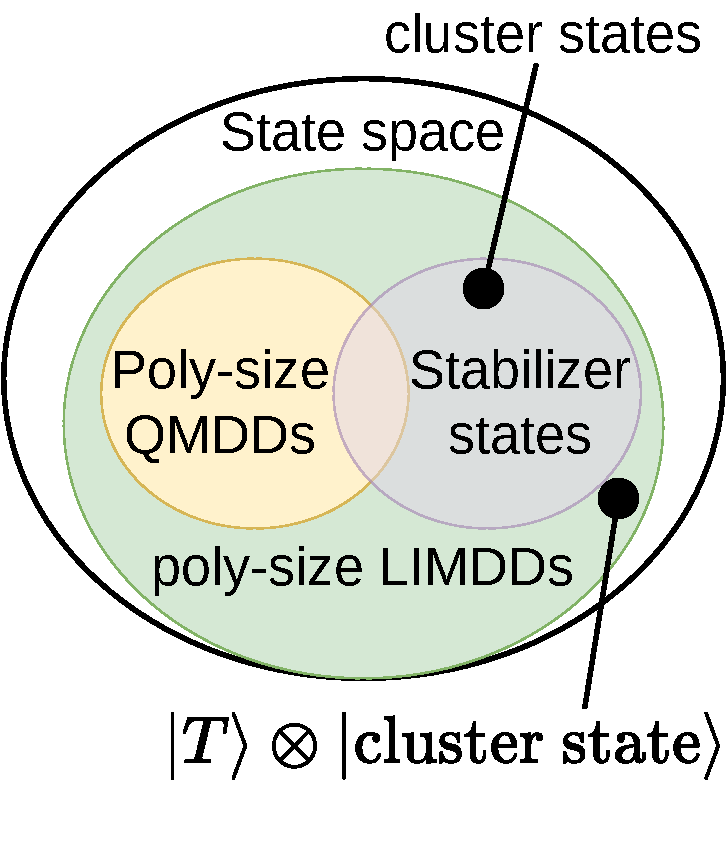
\includegraphics[width=.24\textwidth]{pics/venn-diagram.pdf}
    \centering
    \vspace{-1em}
	\caption{
        The set of stabilizer states and states represented as:
        poly-sized \limdds and QMDDs.
        \vspace{-\baselineskip}
	}%\vspace{-.5em}
    \label{fig:venn-diagram} 
\end{wrapfigure}

Another method for simulating universal quantum computation is based on (algebraic) decision diagrams (DDs)~\cite{akers1978binary,bryant86,580054,bryant1995verification,sanner,10.1145/157485.164569,fujita1997multi,viamontes2003improving,viamontes2004high,miller2006qmdd,zulehner2018advanced}.
A DD is a directed acyclic graph (DAG) in which each path represents a quantum amplitude, enabling the succinct representation of many quantum states through the combinatorial nature of these paths.
Various manipulation operations for DDs exist which implement any quantum gate operation in polynomial time
in the size of the DD. Together with other DD operations that can be used for measurement,
strong simulation is easily implemented using a DD data structure~\cite{miller2006qmdd,zulehner2018advanced}.
Indeed, DD-based simulation was empirically shown to be competitive with state-of-the-art simulators~\cite{viamontes2004high,zulehner2018advanced} and is used in several simulator implementations~\cite{viamontes2009quantum}.
%\todo{Vedran: at-the time? I mean, simulators have advanced a lot since 2018... As I mentioned they simulated shor on 60 qubits. good luck with that in any other method.}.
DDs and the stabilizer formalism are introduced in \autoref{sec:preliminaries}.
%However, in contrast to the stabilizer formalism, little is known about which quantum circuits are efficiently simulatable with DD-based approaches.


In this paper, we show that certain stabilizer states, called cluster states \cite{briegel2000persistent}, yield exponentially large \qmdds, the currently most succinct version of DDs
(see \autoref{sec:exponential-separations}).
In order to unite the strengths of DDs and the stabilizer formalism,
in \autoref{sec:isomorphism-qmdd}, we propose \limdd: a new DD for quantum computing simulation using local invertible maps (LIMs).
Specifically, \limdds eliminate the need to store multiple states which are equivalent up to LIMs, allowing more succinct DD representations.
%\todo{Tim: please check, it might sound a bit like \limdds only can encode stabilizer states now}
We prove that the set of quantum states that can be \emph{represented} by poly-sized \limdds 
is larger than those that can be expressed in either the stabilizer formalism or a poly-sized \qmdd.
\autoref{fig:venn-diagram} shows the resulting separation.
In \autoref{sec:quantum-simulation}, we give procedures for analyzing and simulating quantum 
circuits using \limdds and conclude in \autoref{sec:discussion} with evidence that \limdd-based simulation can be powerful than modern techniques using low-rank stabilizer decomposition~\cite{bravyi2019simulation}.

The workhorse behind \limdds is a novel algorithm which merges two DD nodes when they are `isomorphic:'
Two quantum states $\ket{\phi}$ and $\ket{\psi}$ are isomorphic when there is a series of Pauli operators $P_j$ and a complex nonzero number $\lambda$ such that $\ket{\phi}=\lambda P_n\otimes\cdots\otimes P_1\ket \psi$.
There is a plethora of work on investigating the effect of similar local operations in the context of stabilizer states \cite{nest2005local, englbrecht2020symmetries}; we emphasize that here we consider arbitrary quantum states $\ket{\phi}, \ket{\psi}$.%\todo{Tim: should rephrase, now it looks like no-one ever thought of considering locally-equivalent states beyond stabilizer states...}
To find such an isomorphism, we compute (generators of) the stabilizer (sub)group $\Stab(\ket \psi)$ of the state $\ket \psi$ represented by each DD node, and then we exploit the fact that the set of all such isomorphisms can be expressed as the coset $\pi\cdot \Stab(\ket \psi)$ for some isomorphism $\pi$.
To make the diagram canonical ---an important property for realizing efficient manipulation operations~\cite{darwiche2002knowledge}---
our algorithm then chooses a ``lexicographically smallest'' element from a Pauli coset.

%\todo[inline]{Vedran: general comment: i am a bit worried that nothing about efficiency of algorithms for all the manipulations is said for such a long time... I lose the connection to simulation of circuits... The Introduction for me is missing a link and clarification of the relationship between representation and simulation."}


%\todo[inline]{Give another / better example of polytime simulatable QC; introduce stabilizer states before they are mentioned.}

%\todo[inline]{Process Vedran's feedback, so write something about Clifford gates that's actually true.}

%This work is organized as follows.
%After providing the necessary background in \autoref{sec:preliminaries}, we formally introduce \limdds in \autoref{sec:isomorphism-qmdd}.
%In \autoref{sec:exponential-separations}, we prove the exponential separation between QMDDs and \limdds, by showing that there is a sequence of $n$-qubit stabilizer states that can only be represented with exponentially-sized QMDDs.







\section{Preliminaries: decision diagrams and stabilizer states \label{sec:preliminaries}}
%\todo[inline]{mention terminology `low' and `high' for 0-edge and 1-edge}

%Here, we briefly introduce two methods to manipulate and succinctly represent quantum states: decision diagrams and stabilizer states.
%For an introduction to quantum computation, see appendix~\ref{sec:quantum-nutshell}.

The computational unit of quantum computers are quantum bits or qubits.
A single-qubit state is a complex vector $(\alpha_0, \alpha_1)^{T} \in \mathbb{C}^2$ with norm 1, usually written in Dirac notation as $\alpha_0 \ket{0} + \alpha_1 \ket{1}$.
Two quantum states which differ only by a complex multiple are considered equal.
The joint state $\ket{\phi}$ of $n$ quantum bits can be written as 
\begin{equation}
    \label{eq:quantum-state-expansion}
    \sum_{x_1, x_2, \dots, x_n \in \set{0,1}} f(x_1, x_2, \dots, x_n) \ket{x_1}\otimes\ket{x_2}\otimes \dots \otimes\ket{x_n}\vspace{-1em}
\end{equation}
for a function $f: \{0, 1\}^n \rightarrow \mathbb{C}$, where $\otimes$ denotes the tensor product.
An example two-qubit state is $\left( \ket{0} \otimes \ket{0} + i \ket{1} \otimes \ket{1}\right) / \sqrt{2} = \frac{1}{\sqrt{2}} (1,0,0,i)^T$.
Alternatively to \autoref{eq:quantum-state-expansion}, we can recursively describe an $n$-qubit quantum state $\ket{\phi}$ for $n>1$ as
\begin{equation}
\ket{\phi} = \alpha_0 \ket{0} \otimes \ket{\phi_0} + \alpha_1 \ket{1} \otimes \ket{\phi_1}, \text{where $\ket{\phi_0}, \ket{\phi_1}$ are $n$-1-qubit states and $\alpha_0,\alpha_1  \in \mathbb{C}$.}
    \label{eq:quantum-state-recursive}
\end{equation}
An Algebraic Decision Diagram (\add) represents a function of the form $f\colon \{0, 1\}^n \rightarrow \mathbb{C}$, and thus also a quantum state via \autoref{eq:quantum-state-expansion}, see \autoref{fig:qmdd-isoqmdd-exposition} for an example.
%A succint representation of functions of the form $f\colon \{0, 1\}^n \rightarrow \mathbb{C}$, and thus of quantum states via \autoref{eq:quantum-state-expansion}, has been achieved by the use of Algebraic Decision Diagrams (\adds), see \autoref{fig:qmdd-isoqmdd-exposition} for an example.
An \add is a rooted directed acyclic graph (DAG), which has a leaf node for each unique value in the image of $f$, i.e., in $\{f(\vec{x}) \mid \vec{x} \in \{0, 1\}^n \}$.
Each path from the root to a leaf visits nodes representing the variables $x_1, x_2, x_3, x_4$; one variable at each level of the diagram.
The value $f(x_1, \dots, x_n)$ is found by traversing such a path, following the \concept{low edge} (dashed line)
 when $x_i=0$, and the  \concept{high edge} (solid line) when $x_i=1$;
 so, e.g., $f(1,1,1,0) = -i$ in \autoref{fig:qmdd-isoqmdd-exposition}.
Hence every node in an \add, not only the root node, can be said to represent a function.

%\adds for functions $f$ on length-$n$ bitstrings can be defined recursively on $n$: in case $n=1$, then the \add has a single node with two outgoing edge, labelled $0$ and $1$ and pointing to the leaf node holding the value $f(0)$ and $f(1)$ respectively.
%If $f(0) = f(1)$, then the \add only has a single leaf node and both edges point to that node.
%If $n>1$, then and \add for $f$ is constructed by first constructing \adds for the two functions $f_0: (x_2, x_3, \dots, x_n) \mapsto f(0, x_2, x_3, \dots, x_n)$ and $f_1: (x_2, x_3, \dots, x_n) \mapsto f(1, x_2, x_3, \dots, x_n)$.
%An \add for $f_0$ is then made by adding a fresh node and a $0$-edge ($1$-edge) pointing to the root node of the \add of $f_0$ (the \add of $f_1$).
%If the \adds of $f_0$ and $f_1$ are identical, then remove one of them and make both edges point to the remaining one.
%Thus, in an \add, the value $f(x_1, \dots, x_n)$ is found by traversing the path $x_1 \rightarrow x_2 \rightarrow \dots \rightarrow x_n$, e.g. $f(1,1,0) = -1/\sqrt{2}$ in \autoref{fig:add-qmdd-example}.
%Although generally, functions $f: \{0, 1\}^n \rightarrow \mathbb{C}$ have exponentially many partial assignments, many functions encountered in practice have only a polynomial number of unique subfunctions, and therefore can be represented by polynomial-size \add.

A \emph{partial assignment} $(x_1=a_1,\ldots, x_k=a_k)$ to the variables induces a \emph{subfunction} $f_a$, defined as $f_a(x_{k+1},\ldots, x_n)\defn f(a_1,\ldots, a_k,x_{k+1},\ldots, x_n)$.
Two \add nodes representing the same subfunction can be \emph{merged}, i.e., one node is deleted and its incident edges are rerouted to the other.
When all eligible nodes have been merged, an \add is \emph{reduced}.
The nodes of a reduced \add are in one-to-one correspondence with the unique \emph{subfunctions} of $f$.
An \add is a \emph{canonical} representation: a given function has exactly one reduced \add.
\adds can represent both states and matrices, and there are algorithms which multiply a matrix with a vector in \add form.
An \add can represent any quantum state, using exponentially many nodes in the worst case.
A given quantum gate can be compiled into an \add, thus allowing one to simulate any quantum circuit by repeatedly multiplying a gate's matrix with a state. %\todo[inline]{@Lieuwe: David asks for ref here}
%For example, the functions $(x_2, x_2, \dots, x_n) \mapsto f(0, x_2, x_3, \dots, x_n)$ and $(x_4, x_5, \dots, x_n) \mapsto f(0, 1, 1, x_4, x_5, \dots, x_n)$ are subfunctions of $f$.
%At a node in an \add corresponding to the $k$-th variable, the two outgoing arrows correspond to the partial assignments $x_k=0$ and $x_k=1$.

The Quantum Multi-valued Decision Diagram (\qmdd) \cite{miller2006qmdd} improves on the \add representation by also merging two nodes when they represent functions $f,g$ that are related by $f=\lambda\cdot g$ for some $\lambda\in\mathbb C^{\ast}$.
\autoref{fig:qmdd-isoqmdd-exposition} gives an example.
Each edge is labelled with a weight. % (the normalization constant $\lambda$).%$^{\ref{fn:norm}}$
To read a value of $f$, traverse the \qmdd from the root to the leaf just as in an \add, and multiply the weights of all edges on that path.
Like \adds, \qmdds are a canonical representation and can be used to simulate any quantum circuit.

The single-qubit Pauli operators are
$2\times 2$ unitary matrices:
\begin{equation*}
\id[2] \defn \begin{pmatrix} 1 & 0\\ 0 & 1 \end{pmatrix},
X \defn \begin{pmatrix} 0 & 1\\ 1 & 0 \end{pmatrix},
Y \defn \begin{pmatrix} 0 & -i\\ i & 0 \end{pmatrix},
Z \defn \begin{pmatrix} 1 & 0\\ 0 & -1 \end{pmatrix}
\label{eq:pauli-matrices}
\end{equation*}
where $i$ is the complex unit.
An $n$-qubit operator of the form $P_n\otimes\cdots\otimes P_1$ is called a \emph{Pauli string} if $P_j$ are single-qubit Pauli operators.
The $n$-qubit Pauli strings generate a nonabelian group $\Pauli_n$ (under matrix multiplication), consisting of all operators of the form $\lambda P_n\otimes\cdots\otimes P_1$ with $\lambda \in \{\pm 1, \pm i\}$.
Note that the high indices are on the left, in keeping with the custom that the least significant (qu)bit is the first qubit, and the leftmost operator $P_n$ acts on the most significant qubit. 
Pauli operators $A, B$ either commute ($A\cdot B = B\cdot A$) or anticommute ($A \cdot B = - B \cdot A$).

In contrast to decision diagrams, the stabilizer formalism forms a subset of quantum computation that is efficiently simulatable.
A stabilizer state on $n$ qubits can be prepared from the state $\ket{0}^{\otimes n}$ by repeatedly applying any of the following gates (generators of the Clifford set):
\begin{equation}
    H \defn 
        \frac{1}{\sqrt{2}}
        \begin{pmatrix} 1 & 1\\ 1 & -1 \end{pmatrix}
            ,
        S
        \defn
        \begin{pmatrix} 1 & 0\\ 0 & i \end{pmatrix},
            \textnormal{CNOT} \defn 
        \begin{pmatrix}
            1 & 0 & 0 & 0\\
            0 & 1 & 0 & 0\\
            0 & 0 & 0 & 1\\
            0 & 0 & 1 & 0
        \end{pmatrix}.
        \label{eq:clifford-generators}
\end{equation}
There exist $2^{\Theta(n^2)}$ stabilizer states on $n$ qubits \cite{aaronson2008improved}; examples are $\ket{00}$ and $(\ket{00} + \ket{11}) / \sqrt{2}$.
A strict subset of stabilizer states is the set of graph states \cite{hein2006entanglement}.
The relationship between graph states and stabilizer states has been extensively investigated in, e.g., \cite{nest2004graphical,nest2005local}
%\todo{Move to S4.1?}
For an undirected graph $G=(V,E)$, the graph state $\ket{G}$ is the following state on $n$ qubits, where $Z_{jk}$ denotes the controlled $Z$-gate between qubits $j$ and $k$.
\begin{equation}
    \frac{1}{\sqrt{2}^n} \prod_{(j, k) \in E} Z_{jk} \left(\ket{0} + \ket{1}\right)^{\otimes n}, \text{ where e.g. }
        Z_{1,2} = 
        \begin{pmatrix}
            1 & 0 & 0 & 0\\
            0 & 1 & 0 & 0\\
            0 & 0 & 1 & 0\\
            0 & 0 & 0 & -1
        \end{pmatrix} \text{ for } n=2.
	\label{eq:graph-state-definition}
\end{equation}
%Although not every stabilizer state is a graph state, any stabilizer state can be converted into one by local Cliffords (LC)~\cite{nest2004graphical}.
%Moreover, since LC-equivalence between two graphs is efficient~\cite{nest2005local}, so is LC-equivalence between stabilizer states.\todo{Tim: Vedran mentioned this and I added it here, but I am not so sure this is the right place to mention this... All Paulis are CLiffords so checking local-Pauli equivalence is easy for stabilizer states, but we consider arbitrary states...}
An $n$-qubit stabilizer state $\ket{\phi}$ is uniquely specified by the set $S$ of Pauli operators $A \in \Pauli_n$ for which $A\ket{\phi} = \ket{\phi}$.
This set $S$ is an abelian group of $2^n$ elements, succinctly represented by $n$ independent generators.
Since each Pauli generator takes $\mathcal{O}(n)$ space to represent, an $n$-qubit stabilizer is represented by $\mathcal O(n^2)$ bits.
Updating the stabilizer generating set after application of one of the gates from eq.~\eqref{eq:clifford-generators} or a single-qubit computational-basis measurement can be done in polynomial time \cite{gottesman1998heisenberg}.
Also, we note that multiplying two $n$-qubit Pauli strings can be done in $O(n)$ time by using the property of the tensor product $\otimes$ that $(a\otimes b) \cdot (c\otimes d) = (a\cdot c) \otimes (b\cdot d)$.

Stabilizer-rank based methods~\cite{bravyi2016trading,bravyi2017improved,bravyi2019simulation, huang2019approximate,kocia2018stationary,kocia2020improved} extend this approach to families of Clifford circuits with arbitrary input states $\ket{\phi_n}$, enabling the simulation of universal quantum computation in general~\cite{bravyi2005universal}.
By decomposing $\ket{\phi_n}$ as linear combination of $\chi$ stabilizer states, the measurement outcome probabilities can be computed in time $\oh(\chi \cdot \textnormal{poly}(n))$, where the least $\chi$ is referred to as the \concept{stabilizer rank}.
Therefore, stabilizer-rank based methods are efficient for a family of input states $\ket{\phi_n}$ with a stabilizer rank polynomially growing~in~$n$.

In this work we will also consider stabilizer groups of states which are not stabilizer states.
In general, we will refer to an abelian subgroup of $\Pauli_n$, not containing $-\id[2]^{\otimes n}$, as an $n$-qubit \emph{stabilizer subgroup}, which generally has $\leq n$ generators.
Such objects are also studied in the context of simulating mixed states \cite{audenaert2005entanglement} and quantum error correction~\cite{gottesman1997stabilizer}.
Examples of stabilizer subgroups are $\{\id[2]\}$ for $\ket{0} + e^{i\pi/4}\ket{1}$, $\langle -Z\rangle$ for $\ket{1}$ and $\langle X \otimes X\rangle$ for $(\ket{00} + \ket{11}) + 2(\ket{01} + \ket{10})$.

Any $n$-qubit Pauli string can (modulo factor $\in \{\pm 1, \pm i\}$) be written as $(X^{x_n} Z^{z_n}) \otimes \dots \otimes (X^{x_1} Z^{z_1})$ for bits $x_j, z_j, 1 \leq j \leq n$.
We can therefore write an $n$-qubit Pauli string $P$ as length-$2n$ binary vector 
\[
    (\underbrace{x_n, x_{n-1}, \dots x_1}_{\textnormal{X block}} | \underbrace{z_n, z_{n-1}, \dots, z_1}_{\textnormal{Z block}})
    ,
\] 
where we added the horizontal bar ($|$) only to guide the eye.
We will refer to such vectors as \emph{check vectors}.
For example $X \sim (1, 0)$ and $Z \otimes Y \sim (0, 1 | 1, 1)$ \cite{aaronson2008improved}.
A set of $k$ Pauli strings thus can be written as $2n\times k$ binary matrix, often called \emph{check matrix}, e.g.
\[
    \begin{pmatrix}
        X &\otimes& X &\otimes& X\\
        \id[2] &\otimes& Z &\otimes& Y
    \end{pmatrix}
    \sim
    \begin{pmatrix}
        1& 1& 1& |& 0& 0& 0\\
        0& 0& 1& |& 0& 1& 1
    \end{pmatrix}
    .
\]
This equivalence induces an ordering on Pauli strings following the lexicographic ordering on bit strings. %, defined as $\vec{y} \leq \vec{z}$ if either $\vec{y} = \vec{z}$ or else if $\vec{y}$ $\vec{z}$ agree on the first $k$ elements but $\vec{y}_{k+1} < \vec{z}_{k+1}$, where $0<1$.
For example, $X<Y$ because $(1|0) < (1|1)$ and $Z\otimes \id[2] < Z \otimes X$ because $(0 0 | 1 0) < (0 1 | 1 0)$.
Furthermore, if $P, Q$ are Pauli strings corresponding to binary vectors $\vec{x}^P, \vec{z}^P$ and $\vec{x}^Q, \vec{z}^Q$, then 
\[
P \cdot Q \propto
\bigotimes_{j=1}^n
\left(X^{x^P_j} Z^{z^P_j}\right) \left(X^{x^Q_j} Z^{z^Q_j}\right) 
=
\bigotimes_{j=1}^n
\left(X^{x^P_j \oplus x^Q_j } Z^{z^P_j \oplus z^Q_j} \right)
\]
and therefore the group of $n$-qubit Pauli strings with multiplication (disregarding factors) is group isomorphic to the vector space $\{0, 1\}^{2n}$ with bitwise addition (i.e., exclusive or; `xor').
Consequently, many efficient algorithms for linear-algebra problems carry over to sets of Pauli strings.
In particular, if $G = \{g_1, \dots, g_k\}$ are length$-2n$ binary vectors (/ $n$-qubit Pauli strings) with $k\leq n$, then we can efficiently perform the following operations.
\begin{description}
%    \item[\emph{Orthogonalization:}] convert $G$ to a (potentially smaller) independent set, using the Gram-Schmidt procedure, in $O(n^3)$ time.
    \item[\emph{RREF:}] bring $G$ into a reduced-row echelon form (RREF) using Gauss-Jordan elimination (both standard linear algebra notions) where each row (in check matrix form) has strictly more leading zeroes than the row above.
        The RREF is achievable by $O(k^2)$ row additions (/~multiplications modulo factor) and thus $O(k^2 \cdot n)$ time (see \cite{berg2020circuit} for a similar algorithm).
        In the RREF, the first $1$ after the leading zeroes in a row is called a `pivot'.
    \item[\emph{Independent Set}] convert $G$ to a (potentially smaller) independent set by performing the RREF procedure and discarding resulting all-zero rows.
    \item[\emph{Membership:}] determining whether a given a vector (/~Pauli string) $h$ has a decomposition in elements of $G$.
        This task can be reduced to independence by first getting $G^{\textnormal{RREF}}$ by applying RREF, followed by adding $h$ to $G$ and performing the Independent-Set procedure. The result has $|G^{\textnormal{RREF}}|$ rows if $h\in \langle G\rangle$, and $|G^{\textnormal{RREF}}| + 1$ rows otherwise.
    \item[\emph{Intersection:}] determine all Pauli strings which, modulo a factor, are contained in both $G_A$ and $G_B$, where $G_A, G_B$ are generator sets for $n$-qubit stabilizer subgroups.
        This can be achieved using the Zassenhaus algorithm \cite{LUKS1997335} in time $O(n^3)$.
    \item[\emph{Division remainder:}] given a vector $h$  (/~Pauli string $h$), determine \mbox{$ h^{\textnormal{rem}} := \min_{g\in \langle G\rangle} \{ g  h\}$} (minimum in the lexicographic ordering) where $\oplus$ denotes bitwise XOR (/~factor-discarding multiplication).
        We do so in the check matrix picture by bringing $G$ into RREF, and then making the check vector of $h$ contain as many zeroes as possible by adding rows from $G$:
	\begin{algorithmic}[1]
        \For{column index $j=1$ to $2n$}
        \If{$h_j = 1$ and $G$ has a row $g_i$ with its pivot at position $j$}
		$h := h \oplus g_i$
        \EndIf
        \EndFor
	\end{algorithmic}
        The resulting  $h$ is $h^{\textnormal{rem}}$.
This algorithm's runtime is dominated by the RREF step; $O(n^3)$.
        %\todo{It is hard to follow. An example might help. Perhaps indeed explain where you need it?}
%        \todo[inline]{Tim: this algorithm is obvious but I have not been able to find a reference.... Need to move to elsewhere?}
% AL: I like this overview. If it is trivial let's leave it here. People might still refer to it, and we avoid claiming trivial stuff.
\end{description}

In this work, we will consider the group of $n$-qubit Pauli operators $\lambda P_n \otimes \dots P_n$ for arbitrary $\lambda \in \mathbb{C}-\{0\}$, denoted as $\paulilim_n$.
Since each stabilizer $\lambda P \in \paulilim_n$ has factor $\lambda =\pm 1$ (follows from
$ (\lambda P)\ket{\phi} = (\lambda P)^2 \ket{\phi} =  \lambda^2 \id \ket{\phi}  =\ket{\phi}$, hence $\lambda^2 = 1$), the stabilizer subgroups in $\paulilim_n$ are the same as in $\pauli_n$.
As extension of the check matrix form to $A \in \paulilim_n$, we write $A = r \cdot e^{i\theta} \cdot P_n \otimes ...\otimes P_1$, for $r \in \mathbb{R}_{> 0}$ and $\theta\in [0, 2\pi)$ and represent $A$ by a length-$(2n+2)$ vector where the last entries store $r$ and $\theta$, e.g.:
\[
    \begin{pmatrix}
        3X &\otimes& X &\otimes& X\\
        -\frac{1}{2} i\id[2] &\otimes& Z &\otimes& Y
    \end{pmatrix}
    \sim
    \begin{pmatrix}
        1& 1& 1& |& 0& 0& 0& |&3 & 0\\
        0& 0& 1& |& 0& 1& 1& |&\frac{1}{2} & \frac{3\pi}{2}
    \end{pmatrix}
\]
where we used $3 = 3\cdot e^{i\cdot 0}$ and $-\frac{1}{2}i = \frac{1}{2} \cdot e^{3\pi i/2}$.
The ordering on real numbers induces a lexicographic ordering (from left to right) on such extended check vectors, for example $(1, 1, | 0, 0 | 3, \frac{1}{2} ) < (1, 1 | 1, 0 | 2, 0)$.
Let us stress that the factor encoding $(r, \theta)$ is less significant than the Pauli string encoding $(x_n, \dots, x_1 | z_n, \dots, z_1)$.
As a consequence, we can greedily determine the minimum of two Pauli operators.
%We state this remark separately because we will explicitly use it for proving correctness of our algorithms in~\autoref{sec:choose-canonical-isomorphism-pauli}--\ref{sec:pauli-isomorphism-detection}.

%\def\rp{r}
%\def\thetap{\theta}
%\def\rq{r'}
%\def\thetaq{\theta'}
%\begin{remark}
%    \label{remark:ordering}
%    Checking which of two Pauli operators $\rp e^{i\thetap} P, \rq e^{i\thetaq} P' \in \paulilim_n$ is smaller can be performed in two greedy steps: first, declare $\rp e^{i\thetap} P <  \rq e^{i\thetaq} P'$ if $P < P'$.
%    Otherwise (i.e., if $P = P'$), then proceed to comparing the factors and declare $\rp e^{i\thetap} P <  \rq e^{i\thetaq} P'$ if and only if $(\rp, \thetap) < (\rq, \thetaq)$.
%\end{remark}

Finally, we emphasize that the algorithms above rely on row addition, which is a commutative operation.
%are correct because Pauli operators with factor-ignoring multiplication are group isomorphic to binary vectors with xor.
Since conventional (i.e., factor-respecting) multiplication of Pauli operators is not commutative, the algorithms above are not straightforwardly applicable to (nonabelian subgroups of) $\paulilim_n$.
(For abelian subgroups of $\paulilim_n$, such as stabilizer subgroups \cite{aaronson2008improved}, the algorithms still do work.)
Fortunately, since Pauli strings either commute or anti-commute, row addition may only yield an factors up to the $\pm$ sign, not the resulting Pauli strings.
This feature, combined with the stipulated order assigning least significance to the factor,
enables us to invoke the algorithms above as subroutine, with postpocessing to obtain the correct factor.
We will do so in~\autoref{sec:choose-canonical-isomorphism-pauli}--\ref{sec:pauli-isomorphism-detection}.
%
%
%, which may yield incorrect output (for example, the intersection of $\langle Z \rangle$ and $\langle -Z \rangle$ is $\{\id[2]\}$, while if we discard scalars, the Intersection algorithm above would also return $Z$ as element in the intersection).
%However, because $\paulilim_n$ with factor-respecting multiplication is a non-abelian group while row addition is, there is no commutative row addition operation that preserves factors in the Pauli picture.











%\input{sections/qmdds_for_large_graph_states.tex}


\tikzstyle{e0}[0]=[dotted,bend right=#1]
\tikzstyle{e1}[0]=[solid, bend left =#1]
\defmath\hv{{\hat v}}

\tikzset{every node/.style={initial text={}, inner sep=2pt, outer sep=0}}

\section{The \limdd data structure}
\label{sec:isomorphism-qmdd}


\begin{wrapfigure}{r}{7cm} 
%\begin{figure}
\vspace{-2.5em}
\begin{empheq}[box={\Garybox[Domains of variables]}]{align*}
%\begin{align*}
%\Aboxed{
%\tikzmark{A}
    n, i , j, k                 &\in \mathbb N          && \text{indices} \\
    v, w,u                      &\in \Node     && \text{\limdd nodes}\\
    e, f                           &\in \Edge     && \text{\limdd edges}\\
    L, M                        &\in \textnormal{DD} && \limdd \text{(diagrams)} \\ 
    \ket\phi, \ket\psi                  &\in \mathbb C^{\otimes n}  && \text{$n$-qubit states}\\
    \alpha, \beta, \lambda,\mu  &\in \mathbb C          && \text{complex factors}\\
    P, Q, R                     &\in \Pauli^{\otimes n}&& \text{\pauli strings}\\
    A, B                        &\in \mathbb C \times  \Pauli^{\otimes n}
                                      & & \text{Pauli LIMs}~~~~~~~
%\tikzmark{B}
%}
\end{empheq}
%\tikz[remember picture,overlay]\draw(A.north west)rectangle(B.south east);
%\end{figure}
\vspace{-1em}
\end{wrapfigure}

%The figure on the right lists the default domains of variables used in this paper.

Where \qmdds only merge nodes representing the same state up to a constant factor, the \limdd data structure goes further by also merging nodes that are equivalent up to local operations, called Local Invertible Maps (LIMs) (see \autoref{def:isomorphism}).
As a result, \limdds can be exponentially more succinct than \qmdds, including some stabilizer states (see \autoref{sec:exponential-separations}).
    We will call nodes which are equivalent under LIMs, \emph{(LIM-) isomorphic}.
This definition generalizes SLOCC equivalence; in particular, if we choose the parameter $G$ to be the linear group, then the two notions coincide (Appendix A of \cite{dur2000three})~\cite{bennett1996concentrating,chitambar2014everything}.


\begin{definition}[LIM, Isomorphism]
	\label{def:isomorphism}
    A $n$-qubit Local Invertible Map (LIM) is an operator $\mathcal{O}$ of the form $\mathcal{O}=\lambda \mathcal{O}_n\otimes\cdots\otimes \mathcal{O}_1$, where the matrices $\mathcal{O}_i$ are invertible $2\times 2$ matrices and $\lambda\in\mathbb{C}\setminus \{0\}$.
    An \emph{isomorphism} between two $n$-qubit quantum states $\ket{\phi},\ket{\psi}$ is a LIM $\mathcal{O}$ such that $\mathcal{O}\ket{\phi} = \ket{\psi}$.
    If $G$ is a group of $2\times 2$ invertible matrices and if all $\mathcal{O}_i \in G$, then we say that $\mathcal{O}$ is a $G$-isomorphism and that  $\ket{\phi}$ is $G$-isomorphic to $\ket{\psi}$, denoted $\ket{\phi}\simeq_G\ket{\psi}$.
\end{definition}


Before we give the formal definition of \limdds in \autoref{def:limdd}, we give a motivating example in Figure~\ref{fig:qmdd-isoqmdd-exposition} which demonstrates how the use of isomorphisms can yield small diagrams for a four-qubit state.
%Here a $4$-qubit state is represented in four different ways.
In the state's \qmdd, the nodes $c_3$ and $c_4$ represent the two-qubit state vectors $\ket{c_3}=\left[1,1,1,-1  \right]^\dagger$ and $\ket{c_4}=\left[1,-1,\omega,-\omega  \right]^\dagger$.
By noticing that these two vectors are related via $\ket{c_4}=(T\otimes Z)\ket{c_3}$, we may discard the node $c_4$ and store the isomorphism $T\otimes Z$ instead.
%The state $\ket{c_4}$ can then be recovered from $\ket{c_3}$ by computing $\ket{c_4}=(T\otimes Z)\ket{c_3}$.
% todo LV: ze hebben allemaal andere isomorphisms.
In fact, all the nodes on the \qmdd's third level (i.e., the grandchildren nodes of the root node) are related to each other through such isomorphisms.
A similar reduction in size can be achieved at the \qmdd's second level, by noticing that nodes $c_1$ and $c_2$ are related via $\ket{c_2}=Z\otimes I\otimes Z\ket{c_1}$.
The resulting data structure is a \limdd of only five nodes instead of ten.
\autoref{sec:exponential-separations} shows that discarding isomorphic nodes sometimes leads to exponentially smaller diagrams, while the additional cost of storing the isomorphisms is only polynomial.

\begin{figure}[bh!]
	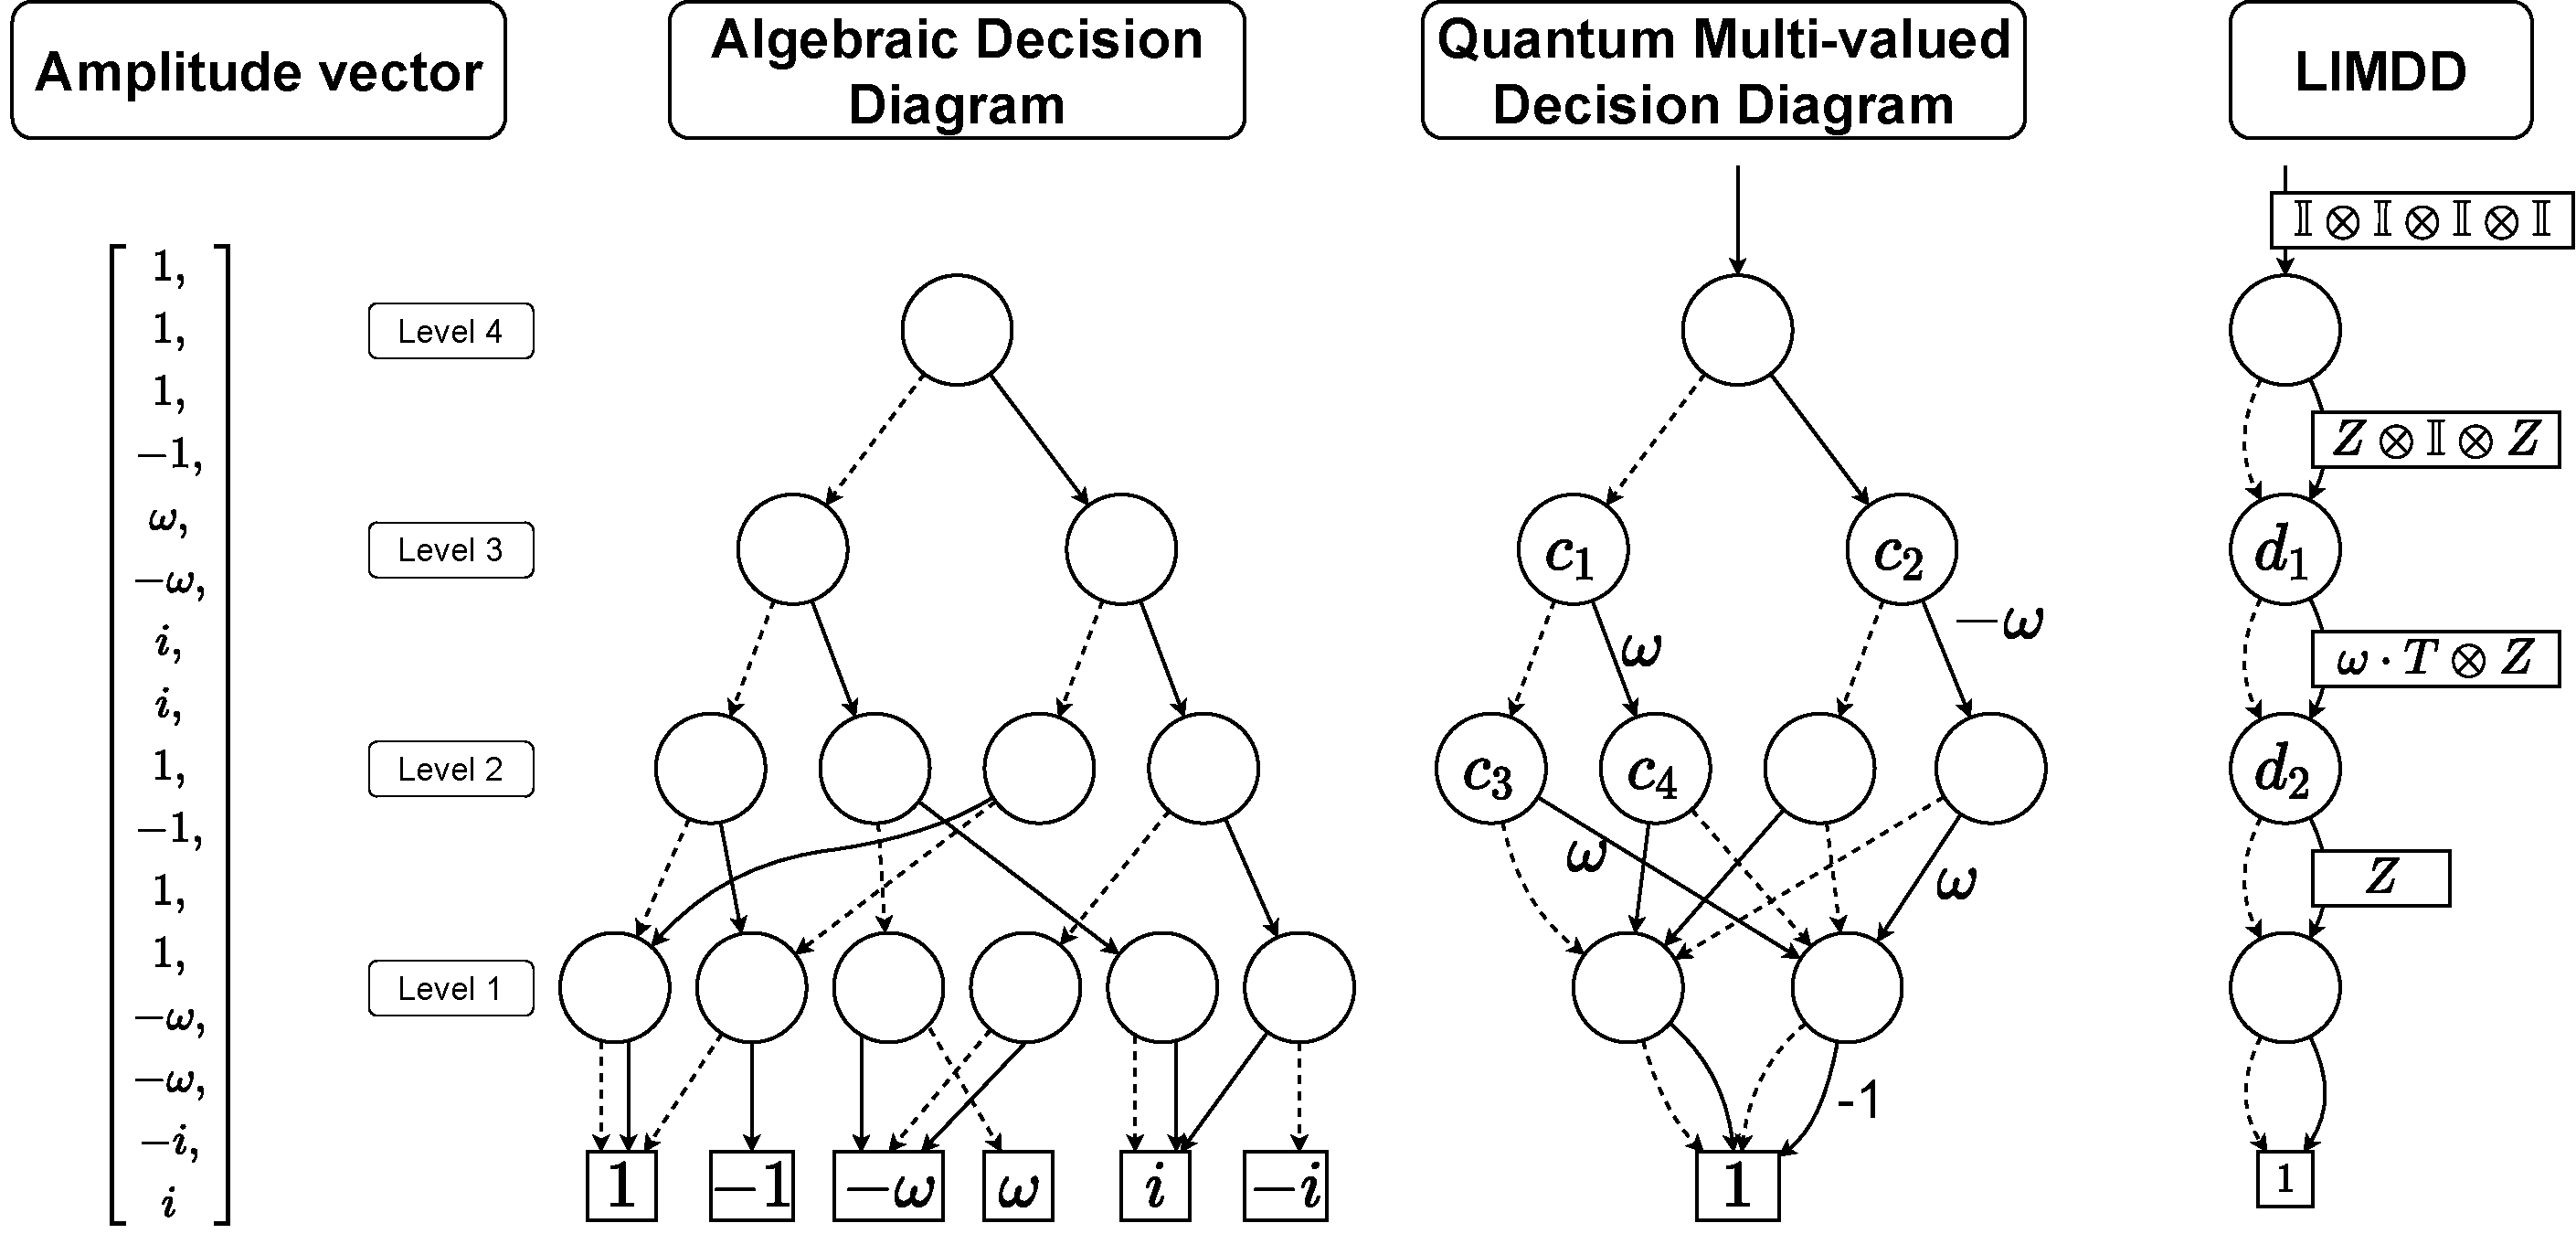
\includegraphics[width=\textwidth]{pics/qmdd-isoqmdd-example-4-qubits-new-notation.pdf}
	\caption{A four-qubit quantum state shown as: an amplitude vector (left), an \add, a \qmdd and a \limdd (right). Diagram nodes are horizontally ordered in `levels' with qubit indices ${4,3,2,1}$.}
	\label{fig:qmdd-isoqmdd-exposition}
\end{figure}

%The formal definition of \limdd is as follows.

\tikzset{every node/.style={initial text={}, inner sep=2pt, outer sep=0}}


\begin{definition}[$G$-\limdd]
	\label{def:limdd}
    An $n$-\glimdd is a rooted, directed acyclic graph (DAG) which represents an $n$-qubit quantum state (or matrix).
    Formally, a \glimdd is a $6$-tuple $(\Node\cup \{\leaf\}, \index,\Low,\High,\lbl,e^r)$,
    where:
\begin{itemize}
	\item $\Node$ is a set of nodes with qubit indices $\index(v) \in [n]$ for $v\in \Node$;
	\item $\Low,\High \colon \Node \to \Node\cup \{\leaf\}$ are the low  and high edge functions;
%	\raisebox{-1mm}{\scalebox{.7}{\tikz{
%		\node[state,minimum size=.2cm] (1) {$v$};
%		\node (-a1) [above left  =.1cm and .3cm of 1] {};
%		\node (-b1) [above right  =.1cm and .3cm of 1] {};
%		\node (1a-) [below left =.1cm and .3cm of 1] {};
%		\node (1b-) [below right = .1cm and .3cm of 1] {};
%		
%		\path[]
%		(-a1) edge node {} (1)
%		(-b1) edge node {} (1)
%		(1) edge node {} (1a-)
%		(1) edge node {} (1b-);
%	}}}.
	\item $\lbl\colon \Low\cup \High\to G$-$\LIM\cup\set 0$ is a function labeling edges with LIMs or $0$;
%       \raisebox{-1mm}{\scalebox{.7}{\tikz{
%            \node[] (1) {};
%            \node [below = .5 of 1] (2) {};
%            \path[] 
%                (1) edge node[right] {$ (\lambda, A_1,\ldots, A_n)$} (2);
%        }}}, and
	\item a root edge $e^r$ without source pointing to root node $r\in \Node$;
%		\raisebox{-1mm}{\scalebox{.7}{\tikz{
%			\node[state,initial,minimum size=.2cm] (r) {$r$}; 
%			\node[below left= .1cm and .3cm of r] (1) {};
%			\node [below right= .1cm and .3cm of r] (2) {};
%			\path[] 
%			(r) edge [dotted] node {} (1)
%			(r) edge [dotted] node {} (2);
%		}}},
    \item a unique leaf node $\leaf$ (a sink) with label $\index(s) = 0$ 
    representing the number $1$;
%        \raisebox{-.5mm}{\scalebox{.7}{\tikz{
%            \node[draw, rectangle,minimum size=.2cm] (s) {$1$}; 
%            \node[above left= .1cm and .3cm of s] (1) {};
%            \node[above= .2cm of s] (a) {};
%            \node [above right= .1cm and .3cm of s] (2) {};
%            \path[] 
%                (1) edge [dotted] node {} (s)
%                (a) edge [dotted] node {} (s)
%                (2) edge [dotted] node {} (s);
%        }}},
%\item If an edge has label $0$, then it points to the leaf node.
%    Otherwise, if $v$ is a node with children $v_0, v_1$, then $\index(v_0) = \index(v_1) = \index(v)-1$;
%        \todo[inline]{note: this used to be the Zero Edges Rule before}
\end{itemize}
Depending on context, we interpret $\lbl(\low v)$ as a node $v_0$ or edge  $(v, v_0)$, etc.
We define the semantics of a (non-leaf) node $v$ and edge $e=(w,v)$  by overloading the Dirac notation:
\begin{align*}
\ket{e} & \defn \begin{cases}
    \lambda \cdot  (\mathcal{Q}_{\index(v)}\otimes \cdots \otimes \mathcal{Q}_1) \cdot \ket v & \text{if $\lbl(e) = (\lambda,  \mathcal{Q}_1, \ldots , \mathcal{Q}_{\index(v)})$} \\
	[0, \dots,0]^\dagger & \text{if $\lbl(e)=0$} \end{cases} \\
\ket{v}     & \defn \ket{0}\otimes\ket{\low v}+ \ket{1}\otimes \ket{\high v}
\end{align*}
\end{definition}

The coefficient $\langle x | e \rangle$ for bitstring $x \in \{0, 1\}^n$ 
of a \limdd with root edge $e$ representing an $n$-qubit state $\ket e$ 
is read by traversing the \limdd from top to bottom according to \autoref{def:limdd}
(i.e., pushing down the LIMs).
It is best illustrated by example, e.g., reading the amplitude for $1111$ in the \limdd of
\autoref{fig:qmdd-isoqmdd-exposition}. The LIM on the root edge is the identity, so we can simply follow the 1-edge to get a new root edge with LIM $P_3\otimes P_2 \otimes P_1 =Z\otimes \id \otimes Z$~to~$d_1$. 
Since the most significant operator ($P_3$) is a $Z$, we multiply the LIM on the 1-edge of $d_1$ (which has $\index(d_1)=3$) with $-1$ and the remainder of the LIM ($\id \otimes Z$),
yielding $ - \omega T \otimes \id$, etc. Eventually the leaf is reached, when only a factor remains (= the sought amplitude).
If we would encounter an $X$ (or $Y$) as $P_3$, we would also have to switch the high (1)
and the low (0) edge, thus taking the 0- instead of 1-edge (and multiply by $-i$ for $P_3 = Y$).
For the choice $G=\Pauli$, this is formalized in the \follow{}{} procedure given in \autoref{sec:quantum-simulation}.

Let us now summarize the representation and manipulation capabilities of the \limdd data structure.
A $G$-\limdd is exact and universal, i.e., for each $n$-qubit quantum state $\ket\phi$ there is a \limdd with root edge $e$ such $\ket e = \ket\phi$, for any choice of parameter $G$.
In particular, a \glimdd with $G=\set{\mathbb I}$ captures all \qmdds by definition.
As all groups $G$ contain the identity operator $\mathbb I$, the universality of \limdds follows from the universality of QMDDs.
Furthermore, for the choice $G=\textsf{Pauli}$, the states that \limdds can represent using polynomial space include all stabilizer states, which is a feature that \qmdds do not posses, as shown in \autoref{sec:exponential-separations}.
Finally, $\textsf{Pauli}$-\limdds can also \emph{manipulate} and measure quantum states, thereby enabling the simulation of quantum circuits, as shown in \autoref{sec:simulation}. 
For many operations, we show that the manipulation is also efficient, i.e., it takes polynomial time in the size of the \limdd representation of the quantum state/circuit.
Specifically, \limdds are often faster than \qmdds, and never slower than a multiplicative factor $O(n^3)$.

From here on, we will focus on the choice $G=\Pauli$, omitting the prefix $\Pauli$- in front of $\limdd$ unless it is clear that we mean otherwise, and hence write $\simeq$ to mean $\simeq_{\textnormal{Pauli}}$.

%From here on, we will focus on the choice $G=\Pauli$, omitting the prefix $\Pauli$- in front of $\limdd$ unless it is clear that we mean otherwise, and hence write $\simeq$ to mean $\simeq_{\textnormal{Pauli}}$.
%For $\Pauli$-\limdds representing an $n$-qubit state $\ket{\phi}$, reading the coefficient $\langle x | \phi\rangle$ of bitstring $x \in \{0, 1\}^n$ is done by traversing the \limdd from top to bottom: at a node with incoming edge label $\lambda P_n \otimes \dots \otimes P_n$, following the $x_k$-edge  if $P_k\ket{x_k} \propto \ket{x_k}$ (e.g. the $0$-edge when $x_k = 0$ and $P_k \in \{\id[2], Z\}$) and the $(1 - x_k)$-edge if $P_k \ket{x_k} \propto \ket{1 - x_k}$ instead (e.g. the $1$-edge when $x_k = 0$ and $P_k \in \{X, Y\}$).
%The coefficient is the product of the factors $\lambda \cdot \langle x_k | P | x_k\rangle$ of the traversed edge labels $\lambda P$.
%For a general group $G$, the coefficients are not encoded in a single path from root to leaf.

%\todo[inline]{Vedran: ok. One may wonder: this is all ok, but how do i compute the amplitude now? It was easy in the QMDD case, I follow the path and multiply numbers...
%	For intuition this is missing for me.
%
%Lieuwe: So do we add an explanation how to compute amplitudes?
%
%Tim: above, I added some text for the case $G=Pauli$, please check.
%}

In general, there are many different $\Pauli$-\limdds which represent a given quantum state.
By imposing a small number of constraints on the diagram, listed in \autoref{def:reduced-limdd} and visualized in \autoref{fig:necessity-of-reduction-rules}, we ensure that every quantum state is represented by a unique `\emph{reduced}' \limdd.
Unique representation, or canonicity, is a useful property of decision diagrams.
In the first place, it allows for circuit analysis and simplification~\cite{bryant1995verification,miller2006qmdd}, by
 facilitating efficient manipulation operations.
In the second place, a reduced diagram is smaller than an unreduced diagram because it merges nodes with the same semantics. For instance, \limdds allow all states in the same $\simeq$ equivalence class to be merged.
The algorithms for quantum circuit simulation in \autoref{sec:quantum-simulation} ensure that all intermediate \limdds are reduced.



%A reduced \limdd representing a state $\ket{\phi}$ has the desirable property that it is the minimum-size diagram among all \limdds representing the state $\ket{\phi}$ (\autoref{thm:reduced-glimdd-minimum-size}).

\begin{definition}[Reduced \limdd]
	\label{def:reduced-limdd}
%	Let $\highlabel,\rootlabel$ and $\beforeq$ be as follows.
%	\begin{itemize}
%		\item The function $\highlabel$ takes as input an $n$-\glimdd node $v$, and outputs an $(n-1)$-$G$-LIM $f(v)$.
%		This function has the property that, if $v$ and $w$ are nodes which satisfy the Low Factoring, Low Precedence and Edge Rules (defined below), and if $\ket{v}\simeq_G\ket{w}$, then $\highlabel(v)=\highlabel(w)$
%		with $\ket v \simeq_G \ket{0}\ket{v_0}+\ket{1}\otimes \highlabel(v)\ket{v_1}$.
%		% and if $\ket{v}=\ket{0}\ket{v_0}+\ket{1}\lbl(\high(v))\ket{v_1}$ then $\ket{v}$ is isomorphic to $\ket{0}\ket{v_0}+\ket{1}\otimes \highlabel(v)\ket{v_1}$.
%		%ALFONS: this seems a corollary of the definition
%		In other words, $\highlabel$ is constant within an isomorphism class.
%		\item The function $\rootlabel$ takes as input a \glimdd{}'s distinguished root edge $e^r$, and outputs a LIM $\rootlabel(e^r)$.
%		This function satisfies the property that, if $e^{r}$ and $e^q$ are the root edges of two \glimdds, and if the root nodes $r$ and $g$ satisfy the reduction rules below except the ``Root edge determinism rule'', and if $\ket{e^r}=\ket{e^q}$, then $\rootlabel(e^r)=\rootlabel(e^q)$.
%		\item $\beforeq$ is a total order on the nodes of the diagram.
%	\end{itemize}
	A \pauli-\limdd is \emph{reduced} when it satisfies the following constraints.
	It is \emph{semi-reduced} if it satisfies all constraints except high determinism.
%	\footnote{}
	\begin{enumerate}
		\item \textbf{Merge: } No two nodes are identical: We say
            two nodes $v,w$ are identical~if $\low v= \low w, \high v = \high w,
                \lbl(\low v)=\lbl(\low w)$, $\lbl(\high v)=\lbl(\high w)$.
		\item \textbf{(Zero) Edge: } Any edge $(v,w) \in \High \cup \Low $
has $\index(v) = \index(w) + 1$, and if $\lbl(v,w)=0$, then both edges point to the same node, i.e., $\high v = \low v = w$.
		\item \textbf{Low Precedence: } For each internal node $v$, we have $\low v \beforeq \high v$, where  $\beforeq$ is a total order on the nodes of the diagram.
		\item \textbf{Low Factoring: } The label on every low edge to a node $v$ is the identity $\id[2]^{\otimes\index(v)}$.
		\item \textbf{High Determinism: } The label on the high edge of any node $v$ is $\highlim =\highlabel(v)$, where $\highlabel$ is a function that takes as input a semi-reduced $n$-{\Pauli}-\limdd node~$v$, and outputs an $(n-1)$-$\Pauli$-LIM $\highlim$
        satisfying
       $\ket v \simeq_{\Pauli} \ket{0}\ket{\low v}+\ket{1}\otimes \highlim\ket{\high v}$.
        Moreover, for any other semi-reduced node $w$ with $\ket{v}\simeq_{\Pauli}\ket{w}$,
         it returns $\highlabel(w) = \highlim$.
		In other words, $\highlabel$ is constant within an isomorphism class.		
%		\item \textbf{Root Edge Determinism: } The label on the root edge is $\rootlabel(e^r)$.
	\end{enumerate}
\end{definition}


\begin{figure}\begin{center}
	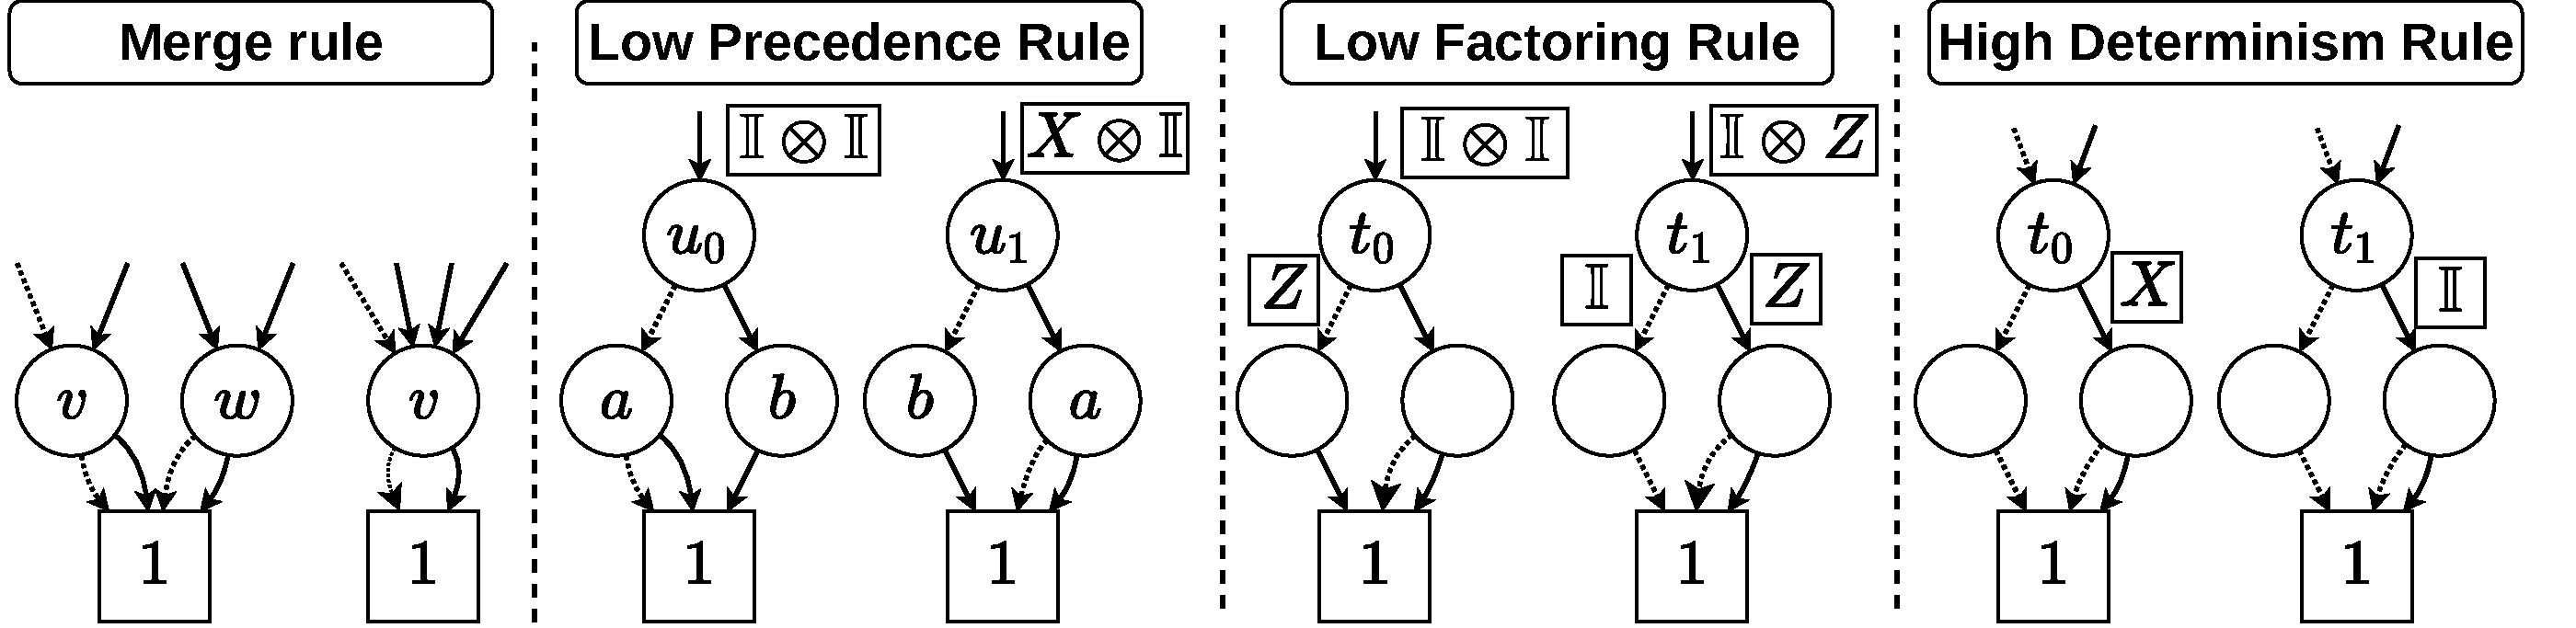
\includegraphics[width=1\textwidth]{pics/necessity-of-reduction-rules.pdf}
	\caption{Illustration of the reduction rules in \autoref{def:reduced-limdd}.
		In each case, the left and right \limdds represent the same state, but the left \limdd violates a reduction rule, while the right \limdd satisfies that rule.
        The Merge rule regards the merging of two identical nodes $v$ and $w$.
		Low Precedence determines which child is the low child, and which is the high child according to~$\beforeq$.
		Low Factoring ensures that the low edge is always labeled with $\mathbb I$.
		High Determinism ensures that the label on high edges is chosen canonically.
		}
	\label{fig:necessity-of-reduction-rules}
\end{center}
\end{figure}

A few observations can be made about the above definition:
	\begin{itemize}
            \setlength\itemsep{1em}
		\item[\namedlabel{obs:nozero}{O1}] There is no reduced \limdd for the $0$-vector, because any low edge must be labeled with~$\id[2]^{\otimes n}$. This is not a problem for us, since the $0$-vector is not a quantum state.
		\item[\namedlabel{obs:knife}{O2}] To represent a state like $\ket{0}\otimes\ket{\phi}$, there is a choice between $\ket{0}\otimes\ket{\phi}$ and $(X\otimes\mathbb I)\ket{1}\otimes \ket{\phi}$.
The low factoring rule forces us to take the $\mathbb I$ label on the low edge, so this gives a node of the form $\ket{0}\otimes \ket{\phi}$. Therefore, the high edge \emph{must} be labeled with $0$. Since, by the zero edges rule, the high edge then points to the same node as the low edge the low precedence rule vacuously holds for such states.
		\item[\namedlabel{obs:subgroups}{O3}] The definition of reduced \limdd cannot always be applied to $G$-\limdd when $G$ is a subgroup of the Pauli group; in particular, such a diagram may not be universal. This is because the low precedence rule requires that $v_0\beforeq v_1$ for every node, so if $G$ is a group which does not contain the $X$, then no reduced \glimdd represents a state $\ket 0 \ket {v_0} + \ket 1 \ket {v_1}$ where $v_1 \beforeq v_0$.
            %In \autoref{sec:exponential-separations}, we come back to this issue.
%            \todo[inline]{Tim: why is this an `issue'? More like a topic, isn't it? Why is it relevant to mention this?}
\item[\namedlabel{obs:delete}{O4}] While the literature on other decision diagrams~\cite{akers1978binary,bryant86,feinstein2011skipped} often considers a ``redundant test'' rule that allows edges to skip multiple levels, we omit this reduction for the sake of simplicity, because it offers only linear improvements in the best case and complicates correctness proofs (see, e.g., \cite[Lemma 1]{andersen1997introduction}). There is however no fundamental reason which would prevent the addition of a similar redundancy reduction.
%	\item[\namedlabel{obs:root-edge}{O5}] the root edge of a diagram may be any LIM; in particular, it is not necessarily equal to $\mathbb I_2^{\otimes n}$.\todo{remove; has nothing to do with reduced.}
%\todo[inline]{This has to be addressed for S4 to work...}
\end{itemize}


\autoref{lemma:node-canonicity-strong} shows that  \limdds are canonical,
in the sense that its nodes 
uniquely represent equivalence classes under $\simeq$ as expressed in \autoref{cor:node-canonicity-strong}. This does not mean that the root edge of a \limdd canonically represents a quantum state. We instead show in \autoref{sec:equality} how to check whether two root edges represent the same state.


%\begin{lemma}
%    [Reduced \limdds have reduced sub-\limdds]
%    \label{lemma:sub}
%    Let $L$ be a \limdd.
%    If the left edge of $v_L$ has label $\unit$, its right edge is labelled $\highlabel(v_L)$ or is labelled zero and points to the same node as its left edge, its children $v_0, v_1$ satisfy Low Precendence, and each node ``under its span'' satisfies the Merge rule, then all these properties also hold for its children.
%\end{lemma}









\begin{corollary}[of \autoref{lemma:node-canonicity-strong}]
    \label{cor:node-canonicity-strong}
    Each equivalence class under $\simeq$, has a unique representative reduced \limdd node $v$, which follows from \autoref{lemma:node-canonicity-strong} and the transitivity of $\simeq$.
\end{corollary}

\begin{lemma}[Node canonicity]
    \label{lemma:node-canonicity-strong}
    For each $n$-qubit state vector $\ket{\phi}$, there exists a unique reduced Pauli-\limdd $L$ with root node $v_L$
    such that $\ket{v_L} \simeq \ket{\phi}$.
%    Isomorphic state vectors are represented by the root node of a unique reduced Pauli-LIMDD.
%    That is, for each state vector $\ket{\phi}$, the set
%    \[
%        C(\ket{\phi}) = \{\textnormal{reduced \limdd L} | \ket{v_L} \simeq \ket{\phi}\}
%    \]
%    satisfies:
%    (a) $C(\ket{\phi}) > 0 $ and (b) $C(\ket{\phi}) \leq 1$.
%    (a) there exists a reduced Pauli-LIMDD $L$ such that $\ket{v_L} \simeq \ket{\phi} \simeq \ket{\psi}$, and
%    : if $\ket{\phi} \simeq \ket{\psi}$, then:
%
%    (b) if there are two reduced Pauli-LIMDDs, with root nodes $v$ and $v'$, then $\ket{v} \simeq \ket{v'} \simeq \ket{\psi}$ implies $v=v'$.
\end{lemma}
\begin{proof}
%	\todo[inline]{From now on, we will write $\simeq$ to mean $\simeq_{\textnormal{Pauli}}$?}
	
    We use induction on on the number of qubits $n$ to show universality (the existence of an isomorphic \limdd node) and uniqueness (canonicity).
%    \todo[inline]{Tim: can't we move proof to appendix?}

%In the lemma's proof, we refer to \limdd DAGs with capitals $L,M$, and their root nodes with $v_L, v_M$.
%Edges to $n$-qubit nodes $v$ in the \limdd carry a Pauli isomorphism $A = \lambda, A_1, \dots, A_n$ according to \autoref{def:limdd}, i.e., a Pauli string interpreted as a LIM $A_n \otimes \dots \otimes A_1$ multiplied by a nonzero complex factor $\lambda$. Note that the factor $\lambda$ can be zero.

    \textbf{Base case.}
    If $n=0$, then $\ket{\phi}$ is a complex number $\lambda$.
    A reduced Pauli-\limdd for this state is the leaf node representing the scalar $1$.
    To show it is unique, consider that nodes $v$ other than the leaf have an $\index(v) > 0$,
    by the edges rule, and hence represent multi-qubit states.
    Since the leaf node itself is defined to be unique, the merge rule is not needed and canonicity follows. Finally, $\ket{\phi}$ is represented by root edge
    $\ledge \lambda1$.
    %
    
    \textbf{Inductive case.}
    Suppose $n>0$.
    We first show existence, and then show uniqueness.
    
    We use the unique expansion of $\ket{\phi}$ as $\ket{\phi} = \ket{0} \otimes \ket{\phi_0} + \ket{1}\otimes \ket{\phi_1}$ where $\ket{\phi_0}$ and $\ket{\phi_1}$ are either $(n-1)$-qubit state vectors, or the all-zero vector.
%    \todo[inline]{Quantum state vectors are defined to be non-zero in \autoref{def:state-vector}, but these vectors are allowed to be zero. -LV}
    We distinguish three cases based on whether $\ket{\phi_0}, \ket{\phi_1} = 0$.

   \textbf{Case $\boldsymbol{\ket{\phi_0}, \ket{\phi_1} = 0}$:}
    This case is ruled out because $\ket{\phi} \neq 0$.

    \textbf{Case $\boldsymbol{\ket{\phi_0}=0}$ or $\boldsymbol{\ket{\phi_1} = 0}$:}
        In case $\ket{\phi_0}\neq 0$,
       by the induction hypothesis, there exists a Pauli-\limdd with root node $w$ satisfying
        $\ket{w} \simeq \ket{\phi_0}$. By definition of $\simeq$,
        there exists an $n$-qubit Pauli isomorphism $A$ such that 
        $\ket{\phi_0} = A \ket{w}$.
       We construct the following reduced Pauli-\limdd for $\ket{\phi}$: 
        $\lnode[v] I{w}0{w}$. 
        In case $\ket{\phi_1}\neq 0$, we do the same for root
            $\ket{w} \simeq \ket{\phi_1} = A \ket w$.
        In both cases, it is easy to check that the root node is reduced.
        Also in both cases, we have $\ket \phi \simeq \ket v$ because 
        either $\ket \phi = \id[2] \otimes A \ket v$ or 
        $\ket \phi = X \otimes A \ket v$ as illustrated in \autoref{fig:reduced1} (left).

\begin{figure}
\tikz[->,>=stealth',shorten >=1pt,auto,node distance=1.5cm,
        thick, state/.style={circle,draw,inner sep=0pt,minimum size=18pt}]{
    \node[state] (1) {$v'$};
    \node[above = .5cm of 1,xshift=1.55cm,fill=black] (x) {};%{$\ket \phi$};
    \node[state] (1a) [below = 1cm of 1, xshift=1.7cm] {$w$};
    
    \path[]
    (x) edge[bend left=-20]     node[above left,pos=.7] {$\id[2]^{\otimes n}$} (1)
    (1) edge[e0,bend left=-20] node[pos=.1,left] {$A$} (1a)
    (1) edge[e1,bend right=-20] node[pos=.1,above right] {$0$} (1a)
    ;

    \node[state, right = 2.5cm of 1] (2) {$v$};
%    \node[above = .5cm of 2] (x)  {$\ket \phi$};%{$= \id[2] \otimes A \ket{v}$};
    \path[]
    (x) edge[bend left=20]     node[above right,pos=.7] {$\id[2] \otimes A$} (2)
    (2) edge[e0,bend left=-20] node[pos=.1,left] {$\id[2]^{\otimes n}$} (1a)
    (2) edge[e1,bend right=-20] node[pos=.2,right] {$0$} (1a)
    (1) --  node[yshift=.1cm] {$\rightsquigarrow$} (2)
    ;
    }~~~~~~~~~~~~~~~
\tikz[->,>=stealth',shorten >=1pt,auto,node distance=1.5cm,
        thick, state/.style={circle,draw,inner sep=0pt,minimum size=18pt}]{
%    \node[above = .5cm of 1] (x) {$\ket \phi$};
    \node[state] (1) {$v''$};
    \node[state] (1a) [below = 1cm of 1, xshift=2.3cm] {$v_L$};
    \node[state] (1b) [below = 1cm of 1, xshift=3.8cm] {$v_R$};
    \path[]
    (1) edge[e0] node[pos=.1,left] {$A$} (1a)
    (1) edge[e1] node[pos=.1,above right] {$B$} (1b)
    (1a) --  node[yshift=-.2cm] {$\beforeq$} (1b)
    ;

    \node[state, right = 2.5cm of 1] (2) {$v'$};
    \node[above = .5cm of 2,fill=black] (x)  {};%{$= \id[2] \otimes A \ket{v'}$};
    \path[]
    (x) edge[bend left=-20]     node[above left,pos=.8] {$\id[2]^{\otimes n}$} (1)
    (x) edge     node[right,pos=.4] {$\id[2] \otimes A$} (2)
    (2) edge[e0] node[pos=.2,left] {$\id[2]^{\otimes n}$} (1a)
    (2) edge[e1] node[pos=.1,right] {$ A^{-1}B$} (1b)
    (1) --  node[yshift=.1cm] {$\rightsquigarrow$} (2)
    ;
    
    \node[state, right = 2.5cm of 2] (3) {$v$};
%    \node[above = .5cm of 3] (x)  {}; %{$ =  (\id[2] \otimes A)\rootlim \ket{v}$};
    \path[]
    (x) edge[bend left=20]      node[above right,pos=.8] {$(\id[2] \otimes A)\rootlim$} (3)
    (3) edge[e0] node[pos=.1,above left] {$\id[2]^{\otimes n}$} (1a)
    (3) edge[e1] node[pos=.2,below right] {$\highlim$} (1b)
    (2) --  node[yshift=.1cm] {$\rightsquigarrow$} (3)
    ;
    }
	\caption{Reduced node construction in case $\ket{\phi_1} = 0$ (left), and
	        $\ket{\phi_0}, \ket{\phi_0} \neq 0$ and $v_L \beforeq v_R$ (right).
	        For cases $\ket{\phi_0} = 0$ and $v_R \beforeq v_L$, we take instead root edge $ X \otimes A$ and swap low/high edges.
	        The black square (\scalebox{.7}{$\blacksquare$})
	        signifies a unique quantum state (all root edge represent this one state).
%            \todo[inline]{Tim: why do we need to show the state above each node? Aren't these obvious from the figure? (i.e. each state is of the form $(rootedge) \ket{rootnode}$}
            }
	\label{fig:reduced1}
\end{figure}

 
    \textbf{Case $\boldsymbol{\ket{\phi_0}, \ket{\phi_1} \neq 0}$:}
    By the induction hypothesis, there exist \pauli-\limdds $L$ and $R$ with root nodes
    $\ket{v_{L}} \simeq \ket{\phi_0}$ and $\ket{v_{R}} \simeq \ket{\phi_1}$.\footnote{Note that the induction hypothesis implies a `local' reduction of \limdds $L$ and $R$, but not automatically a reduction of their union. For instance, $L$ might contain a node $w$ and $R$ a node $w$ such that $v \simeq w$. While the other reduction rules ensure that $v$ and $w$ will be structurally the same, the induction hypothesis only applies the merge rule $L$ and $M$ in isolation, leaving two separate identical nodes $v,w$.
We can solve this by applying merge on the union of nodes in $L$ and $M$, to merge any equivalent nodes.}
    By definition of $\simeq$, there exist $n$-qubit Pauli isomorphisms $A$ and $B$ such that $\ket{\phi_0} = A \ket{v_{L}}$ and $\ket{\phi_1} = B \ket{v_{R}}$.
    In case $v_{L} \beforeq v_{R}$,
       we construct the following reduced Pauli-\limdd for $\ket{\phi}$: the root node is $\lnode[v] {\mathbb I}{v_{L}}E{v_{R}}$, where
    $E$ is the LIM computed by $\highlabel(\lnode{\mathbb I}{v_L}{A^{-1}B}{v_R})$ . 
    Otherwise, if $v_{R}\beforeq v_{L}$, then we construct the following reduced Pauli-\limdd for $\ket{\phi}$: the root node is $\lnode[v] I{v_{R}}F{v_{L}}$, where $F=\highlabel(\lnode{\mathbb I}{v_L}{B^{-1}A}{v_R})$.
    It is straightforward to check that, in both cases, this Pauli-\limdd is reduced.
    Moreover, $\ket v$ isomorphic to $\ket \phi$ 
    as illustrated in \autoref{fig:reduced1} (right).



    To show uniqueness, let $L$ and $M$ be reduced \limdds (root nodes $v_L, v_M$) such that $\ket{v_L} \simeq \ket{\phi} \simeq \ket{v_M}$.
    \def\Ptop{P_{\textnormal{top}}}
    \def\Prest{P_{\textnormal{rest}}}
    Expanding the semantics of $v_L$ and $v_M$, this implies there exists a Pauli isomorphism $\lambda \Ptop \otimes \Prest \neq 0$, where $\Ptop$ is a single-qubit Pauli and $\Prest$ an $(n-1)$-qubit Pauli isomorphism, such that
        \begin{align}
        \label{eq:canonicity-equation-1}
       \lambda \Ptop \otimes \Prest (\ket{0} \otimes A_L \ket{v_L^0} + \ket{1} \otimes B_L \ket{v_L^1})
        =
        \ket{0} \otimes A_M \ket{v_M^0} + \ket{1} \otimes B_M \ket{v_M^1}
        .
        \end{align}

    
    We distinguish two cases from here on: where $\Ptop \in \{\unit, Z\}$ or $\Ptop \in \{X,  Y\}$.
    
    \textbf{Case $\boldsymbol{\Ptop = I,Z}$.}
    If $\Ptop = \diag z$ for $z \in \{1, -1\}$,  then
    \autoref{eq:canonicity-equation-1} gives:
%        \begin{align}
%        \label{eq:canonicity-equation-1}
%       \ket{0} \otimes \lambda\Prest A_L \ket{v_L^0} + \ket{1} \otimes z \lambda\Prest B_L \ket{v_L^1}
%=
%\ket{0} \otimes A_M \ket{v_M^0} + \ket{1} \otimes B_M \ket{v_M^1}
%        \end{align}
        \begin{align}
        \label{eq:canonicity-equation-2}
            \lambda \Prest A_L \ket{v_L^0} = A_M \ket{v_M^0}
            \qquad\textnormal{and}\qquad
            z\lambda \Prest B_L \ket{v_L^1} = B_M \ket{v_M^1}
        \end{align}
            By low factoring, we have $A_L = A_M = \unit$, so we obtain
$ \lambda  \Prest \ket{v_L^0} = \ket{v_M^0}$.      
        Hence $\ket{v_L^0}$ is isomorphic with $\ket{v_M^0}$, so by induction hypothesis and
         \autoref{cor:node-canonicity-strong}, we have $v_L^0 = v_M^0$. 
         We now show that also $v_L = v_M$ by considering two cases.
\begin{description}
        \item[$B_L \neq 0$ and $B_M \neq 0$:] then $z\lambda \Prest B_L\ket{v_L^1}=B_M\ket{v_M^1}$, so the nodes $v_L^1$ and $v_M^1$ represent isomorphic states, so by the induction hypothesis  and \autoref{cor:node-canonicity-strong} we have $v_L^1=v_M^1$.
        We already noticed by the low factoring rule that $v_L$ and $v_M$ have $\mathbb I$ as low edge label.
        By the high edge rule, their high edge labels are $\highlabel(v_L)$ and $\highlabel(v_M)$, and since the reduced \limdds $L$ and $M$ also satisfy low precedence and edge rules and $\ket{v_L} \simeq \ket{v_M}$, we have $\highlabel(v_M) = \highlabel(v_L)$ by definition of $\highlabel$.

        \item[$B_L = 0$ or $B_M= 0$:] In case $B_L = 0$,
        %, then since no state vector has norm 0, we find that $B_M = 0$.
        we see from \autoref{eq:canonicity-equation-2} that $0=B_M\ket{v_M^1}$.
        Since the state vector $\ket{v_M^1}\ne 0$ by \ref{obs:nozero}, it follows that $B_M=0$.
        Otherwise, if $B_M=0$, then \autoref{eq:canonicity-equation-2} yields $z\lambda\Prest B_L\ket{v_L^1}=0$.
        We have $z \lambda\ne 0$, $\Prest \ne 0$ by definition, and $\ket{v_L^1}\ne 0$ by \ref{obs:nozero}.
        Therefore $B_L=0$. In both cases, $B_L=B_M$.
%        Let's first assume $B_L \neq 
\end{description}
        We conclude that in both cases $v_L$ and $v_M$ have the same children and the same edge labels, so they are identical by the merge rule.

        \textbf{Case $\boldsymbol{\Ptop = X, Y}$.}
    If $\Ptop = \begin{smallmat}0 & z^* \\ z & 0\end{smallmat}$ for $z \in \{1, i\}$, then
    \autoref{eq:canonicity-equation-1} gives:
%        \[
%        \ket{1} \otimes z \Prest A_L \ket{v_L^0} + \ket{0} \otimes z \Prest B_L \ket{v_L^1}
%        =
%        \ket{0} \otimes A_M \ket{v_M^0} + \ket{1} \otimes B_M \ket{v_M^1}
%        \]
        \[
            \lambda z\Prest A_L \ket{v_L^0} = B_M \ket{v_M^1}
            \qquad\textnormal{and}\qquad
            \lambda z^*\Prest B_L \ket{v_L^1} = A_M \ket{v_M^0}
            .
        \]
        By low factoring, $A_L = A_M = \unit$, so we obtain 
        $z\lambda  \Prest \ket{v_L^0} = B_M \ket{v_M^1}$
        and
        $\lambda z^*\Prest B_L \ket{v_L^1} = \ket{v_M^0}$.
To show that $v_L = v_M$, we consider two cases.       
\begin{description}
        \item[$B_L \neq 0$ and $B_M \neq 0$:] we find $\ket{v_L^0} \simeq \ket{v_M^1}$ and $\ket{v_L^1} \simeq \ket{v_M^0}$, so by the induction hypothesis, $v_L^0= v_M^1$ and $v_L^1= v_M^0$.
        By low precedence, it must be that $v_L^1 = v_M^1 = v_L^0 = v_M^0$.
        Now use high determinism to infer that $B_L = B_M$ as in the ${\Ptop = I,Z}$ case.
%(NOTE: THIS IS THE SAME CASE AS Case-IZ \& $B_{\Box}$ nonzero. So this is where the root edge rule will help us choose $P=\Ptop \otimes \Prest$)\todo{I don't follow. Root Edge should not be relevant here.}

        \item[$B_L = 0$ or $B_M = 0$:]
       This case leads to a contradiction and thus cannot occur.
        $B_L$ cannot be zero, because then $\ket{v_M^0}$ is the all-zero vector, which we excluded by \ref{obs:nozero}.
        The other case: $B_M = 0$, then it must be that $\Prest$ is zero, hence $\ket{v_M^0}$ is the all-zero vector, which is again excluded.
\end{description}
 We conclude that $v_L$ and $v_M$ have the same children and the same edge labels  for all choices of $\Ptop$, so they are identical by the merge rule.
\end{proof}

%\begin{corollary}[Canonicity]
%    For each $n$-qubit state vector $\ket{\phi}$, there exists a unique Pauli-LIMDD $L$ such that $\ket{e^L} = \ket{\phi}$.
%\end{corollary}
%\begin{proof}
%    By Lemma~\ref{lemma:node-canonicity-strong}, there exists a unique Pauli-LIMDD $M$ such that $\ket{\phi} \simeq \ket{v_M}$.
%    Denote by $P$ a Pauli isomorphism mapping $\ket{v_M}$ to $\ket{\phi}$.
%    As root edge label, we use $\rootlabel(P\cdot e^{v_M})$.
%    By definition of $\rootlabel$, this label choice is unique.
%\end{proof}


%\newpage
%\newpage
%\newpage


% todo the others

%\autoref{thm:limdd-canonicity-root-edge} shows that for every quantum state $\ket{\phi}$, there is indeed a unique reduced \glimdd whose root edge represents $\ket{\phi}$.
%This implies canonicity, since by \autoref{def:limdd}, every \glimdd represents exactly one quantum state.
%
%\todo[inline]{Theorem does not use low precedence, so it is either incorrect or Def 3 is.}
%
%
%%\todo[inline]{Insert figure which shows that, if the reduction rules are NOT obeyed, then we can get multiple diagrams which represent the same state.}
%\begin{figure}[b]
%	\centering
%	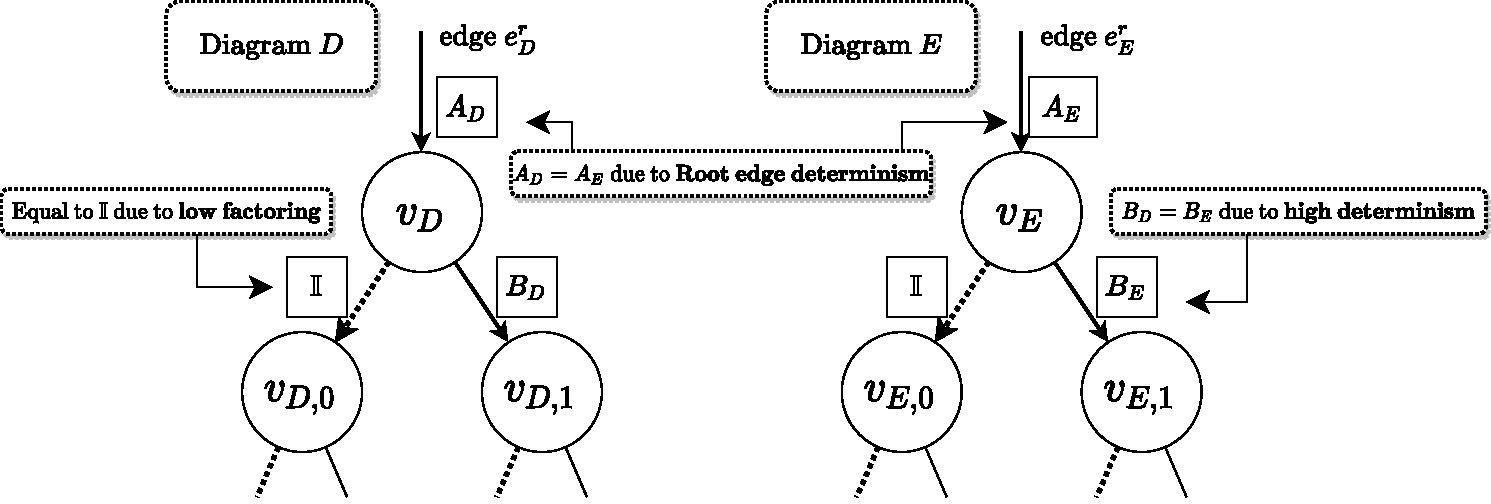
\includegraphics[width=.7\textwidth]{pics/canonicity-two-diagrams.pdf}
%	\caption{Two \glimdds on $n+1$ qubits.}
%	\label{fig:canonicity-two-diagrams}
%\end{figure}
%\begin{theorem}[Canonicity of \glimdd nodes]
%	\label{thm:limdd-canonicity-nodes}
%	If two reduced \glimdd nodes $v_D$ and $v_E$ represent the same state $\ket{v_D}=\ket{v_E}$, and if $G$ is a subgroup of the Dihedral Torus\todo{TODO: Change to Pauli group, or explain exception}, then they are the same diagram.
%\end{theorem}
%\begin{proof}
%	The proof is by induction on the number of qubits.
%	The induction hypothesis is that the theorem holds for all \glimdd nodes on $n$ qubits.
%	
%	\textbf{Base case: $n=0$ qubits. } 
%	There is only one node on $0$ qubits, namely the leaf, representing the scalar $1\in \mathbb C$.
%	Hence, the theorem trivially holds in this case.
%	
%	\textbf{Induction case: $n+1$ qubits. }
%	%	Let $\ket{\phi}$ be a state of $n+1$ qubits, and suppose that two \glimdds $D$ and $E$ represent this state, with $D=(V_D,Low_D,High_D,\textsf{label}_D,e_D^r)$ and $E=(V_E,Low_E,High_E,\textsf{label}_E,e_E^r)$.
%	Suppose that nodes $v_D$ and $v_E$ represent the same $n+1$-qubit state, i.e., $\ket{v_D}=\ket{v_E}$.
%	\alfons{Since $\index(v_D), \index(v_E) = n+1 > 0$, these nodes cannot be leaves.}
%	Hence $v_D$ and $v_E$ are both nodes representing the most significant qubit $n+1$, as implied by the (zero) edges rule\todo{actually requires a few reasoning steps, or we should make it part of the IH},
%	as in \autoref{fig:canonicity-two-diagrams}.
%	%	Say that the diagrams $D$ and $E$ are as in \autoref{fig:canonicity-two-diagrams}.
%	%	In this Figure, the edges $e_D^r$ and $e_E^r$ are labeled with $A_D=\textsf{label}_D(e_D^r)$ and $A_E=\textsf{label}_E(e_E^r)$, and they point to the root nodes $v_D$ and $v_E$, respectively.
%	The node $v_D$ has two (not necessarily distinct) children, $v_{D,0}$ (low) and $v_{D,1}$ (high), and node $v_E$ has children $v_{E,0}$ and $v_{E,1}$.
%	The high edges of nodes $v_D$ and $v_E$ are labeled with $n$-$G$-LIMs $B_D$ and $B_E$, respectively.
%	
%	Since the diagrams $D$ and $E$ are reduced, they satisfy the \emph{Low Factoring}; therefore, the labels on the low edges are $\textsf{label}_D(v_D,v_{D,0})=\textsf{label}_E(v_E,v_{E,0})=\mathbb I$.
%	We show that this implies that $\ket{v_{D,0}}=\ket{v_{E,0}}$.
%	Namely, consider the equation $\ket{v_D}=\ket{v_E}$, and expand the most significant qubit, as follows,
%	\begin{align}
%	\ket{v_D}=\ket{0}\ket{v_{D,0}}+\ket{1}B_D\ket{v_{D,1}} = \ket{0}\ket{v_{E,0}}+\ket{1}B_E\ket{v_{E,1}} = \ket{v_E}
%	\end{align}
%	Since $\ket{0}\ket{v_{D,0}}=\ket{0}\ket{v_{E,0}}$, it follows that $\ket{v_{D,0}}=\ket{v_{E,0}}$.
%	Therefore, by the induction hypothesis, the low children $v_{D,0}$ and $v_{E,0}$ are in fact the same node.
%	
%	
%	The nodes $v_{D}$ and $v_E$ satisfy the \emph{High Determinism Rule}; therefore, the labels on their high edges are equal: $B_D=B_E=\highlabel(v_D)$, because the $\highlabel$ function is constant for nodes representing states in the same equivalence class according to \ref{def:reduced-limdd} and $\ket{v_{D}} = \ket{v_E} \implies \ket{v_{D}} \simeq \ket{v_E}$.
%	%In particular, if $\ket{v}=\ket{0}\ket{v_0}+\ket{1}\lbl(\high(v))\ket{v_1}$ then $\ket{v}$ is isomorphic to $\ket{0}\ket{v_0}+\ket{1}\otimes \highlabel(v)\ket{v_1}$.
%	
%	%\todo{connect to new formalism. Formalize that \highlabel is constant in this case and explain here.}
%	
%	It remains to show that we have $v_{D,1}=v_{E,1}$.
%	To this end, we distinguish two cases: a ``knife'' case, in which $\ket{v_D}=\ket{0}\ket{v_{D,0}}$, and a ``fork'' case.
%	
%	\textbf{Case 1: Knife. }
%	By \autoref{def:reduced-limdd} we have $B_D=B_E=0$.
%	By the zero edge rule, we must have $v_{D,1}=v_{D,0}$ and $v_{E,1}=v_{E,0}$; therefore, we also conclude $v_{D,1}=v_{E,1}$.
%	From the merge rule, we then conclude that the \glimdds $v_D$ and $v_D$ are the same.
%	
%	\textbf{Case 2: Fork. }
%	Since the nodes $v_D$ and $v_E$ represent the same state, consider again the equation $\ket{v_D}=\ket{v_E}$, knowing that $B_D=B_E$:
%	\begin{align}
%	\ket{v_D}=\ket{0}\ket{v_{D,0}}+\ket{1}A_D\ket{v_{D,1}} = \ket{0}\ket{v_{D,0}}+\ket{1}A_D\ket{v_{D,1}} = \ket{v_E}
%	\end{align}
%	It follows that $\ket{1}A_D\ket{v_{D,1}}=\ket{1}A_D\ket{v_{E,1}}$; therefore, in particular $A_D\ket{v_{D,1}}=A_D\ket{v_{E,1}}$.
%	Multiplying both sides with $A_D^{-1}$, we get $\ket{v_{D,1}}=\ket{v_{E,1}}$, i.e., the nodes $v_{D,1}$ and $v_{E,1}$ represent the same state.
%	Therefore, by the induction hypothesis, they must be the same node.
%\end{proof}
%\begin{corollary}
%	\label{thm:limdd-canonicity-root-edge}
%	If root edges $e_D^r, e_E^r$ of reduced \glimdds represent the same state $\ket{e_D^r}=\ket{e_E^r}$, and if $G$ is a subgroup of the Dihedral Torus\todo{tricky}, then they are the same diagram.
%\end{corollary}
%\begin{proof}
%	Since the diagrams $D$ and $E$ are reduced, they satisfy the \emph{Root Edge Determinism Rule}.
%	This means that the labels are chosen as $A_D=\rootlabel(\ket{e_D^r})$ and $A_E=\rootlabel(\ket{e_E^r})$.
%	However, because the diagrams represent the same state, i.e., $\ket{e_D^r}=\ket{e_E^r}$, it follows that $A_D=A_E$, i.e., these two root edges have the same label.
%	
%	It follows that the states represented by the nodes $v_D$ and $v_E$ are the same.
%	Namely, since we have $\ket{e_D^r}=\ket{e_E^r}$, and $\ket{e_D^r}=A_D\ket{v_D}$, and $\ket{e_E^r}=A_D\ket{v_E}$, it follows that $A_D\ket{v_D}=A_D\ket{v_E}$, so, multiplying both sides with $A_D^{-1}$, we get $\ket{v_D}=\ket{v_E}$.
%	By \autoref{thm:limdd-canonicity-nodes}, since the two nodes $v_D$ and $v_E$ represent the same state, they are the same nodes.
%	
%	Because the two \glimdds have the same structure below the root nodes, and have the same label on the root edge, we conclude that they are the same diagram.
%\end{proof}




















%\section{Update PAULI-ISO-QMDD after Clifford unitary}

Roughly: two parts. 1: Update rule for general matrices and general (Pauli group) isomorphism QMDD. 2: Update rule for Clifford gates on Pauli isomorphism QMDDs representing stabilizer states.


\subsection{General update rule}

(We assume that the data structures for vectors and matrices have been described in earlier sections.)

1. Produce $\ket{\psi}:=A\ket{\phi}$, namely  $A\ket{phi_0}$ en $A\ket{phi_1}$. Here $A$ 

2. Check whether the node $\ket{\psi}$ is already in the database.

3. Otherwise, check whether $\ket{\psi}$ is $\mathcal{G}$-isomorphic to a node already in the database. If so, reroute the edges of $\ket{\psi}$ to that node, and delete all newly orphaned nodes.

(Bonus algorithm: Compute expectation values: $\bra{\psi} H \ket{\psi}$. Find a place to put this.)

TODO: Sketch of algorithm on A4.

\subsection{Special update rule}

\subsubsection{Applying a CNOT gate}

1. Update rule for CNOT

2. Try to prune the isomorphism into a single global phase

\subsubsection{Applying a Single-qubit Clifford gate}

1. Expression for Hadamard gate, Phase gate

2. Finding a new isomorphism (work in progress)



(The remainder of this text is old)

Here, we explain briefly why updating Pauli-ISO-QMDDs after a Clifford is nontrivial in the general case.
Below, an algorithm that performs the task is presented

\subsection{Why the Clifford update is nontrivial}

Stabilizer states in Pauli-iso-qmdd has multiple flavours:

\begin{itemize}
\item Z-flavour: read the QMDD as 'in the computational basis'
\item Graph-State-flavour: use Z-flavour but only use Pauli strings containing I and Z (at this point, this flavour precisely contains all graph states), while keeping a list of single-qubit Cliffords that will be applied to the graph state.
\item Pauli-flavour: for each qubit, keep a flag that indicates whether it is stored in the X,Y or Z-basis
\end{itemize}


Performing a single-qubit Clifford in Z-flavour requires an algorithm to update a subpart of the tree with $(\unit + \beta P) / \sqrt{2}$ where $P$ is a Pauli string and $\beta \in \{\pm 1, \pm i\}$.
This follows from a local basis transform, which for example for Z to X-basis follows from the identity
\[
    \ket{0} \otimes \ket{\phi} + \ket{1} \otimes P\ket{\phi}
    = 
    \ket{+} \otimes \frac{\unit + P}{\sqrt{2}} \ket{\phi} + \ket{-} \otimes \frac{\unit - P}{\sqrt{2}}\ket{\phi}
.
\]
CNOTs, on the other hard, are straightforward in Z-flavour.

For Pauli-flavour, the story is reversed: for the same reason, CNOTs are hard but single-qubit Cliffords are trivial.

[For more explanation, see the presentation \url{miscellaneous/2020_05_19_treeform_clifford_update_difficulty.pdf}]



\subsection{An algorithm for the Clifford update}

Here, we sketch how to update a stabilizer state in treeform after application of a single-qubit Clifford or a CNOT.
We use the Z-flavour of treeform, i.e. a stabilizer state on $n$ qubit is recursively defined as $\ket{\phi} = \ket{a} \otimes \ket{\psi}$ or $\ket{\phi} = (\ket{0} \otimes \ket{\psi} + \alpha \ket{1}\otimes \otimes P \ket{\psi}) / \sqrt{2}$, where $a \in \{0, 1, \pm 1, \pm i\}$ and $\alpha \in \{\pm 1, \pm i\}$ and $\ket{\psi}$ is an $n-1$ qubit stabilizer state (or equals $1$ in case $n=1$).

First note that if the most significant qubit is not involved in the application of a Clifford $C$, then in both the knife- and fork cases, it can easily be seen that the Clifford 'propogates' down the tree with little overhead until it meets the first qubit it acts upon:

knife: $C\ket{a} \otimes \ket{\psi} = \ket{a} \otimes \left( C\ket{\psi}\right)$

fork:
$
C \left( \ket{0} \otimes \ket{\psi} + \alpha \ket{1} \otimes Q\ket{\psi}\right)
=
\ket{0} \otimes C\ket{\psi} + \alpha \ket{1} \otimes \left(CQC^{\dagger}\right) \left(C\ket{\psi}\right)
$

\subsubsection{Updating stabilizer state in Treeform after a CNOT}

Denote the stabilizer state by $\ket{\phi}$

\textbf{Claim: updating after a CNOT can be done in time $\mathcal{O}(n^2)$, where $n$ is the number of qubits of $\ket{\phi}$.}

We distinguish two cases.

If $\ket{\phi}$ is a `knife', i.e. $\ket{\phi} = \ket{a} \otimes \ket{\psi}$ for some $a \in \{0, 1, \pm 1, \pm i\}$ and $\ket{\psi}$ is an $(n-1)$-qubit stabilizer state, then the update is straightforward: if $a\in \{0, 1\}$, then the post-CNOT state is a knife and becomes a fork otherwise.
For example, if $\ket{\phi} = \ket{+}\otimes\ket{\psi}$, then $CNOT\ket{\phi} = \ket{0} \ket{\psi} + \ket{1} \otimes X \ket{\psi}$.
(Note we could still ``reduce'' the tree [in the sense of reducing a decision diagram], which we treat below]

If $\ket{\phi}$ is a `fork', i.e. $\ket{\phi} = \ket{0} \otimes \ket{\psi} + \alpha \ket{1}\otimes \otimes P \ket{\psi}$ (omitting normalization), then $CNOT\ket{\phi} = \ket{0} \otimes \ket{\psi} + \alpha \ket{1} \otimes XP \ket{\psi}$.

The only remaining question is: can we reduce this tree?
That is, are the post-CNOT states which are a fork, really a fork or can they also be written as knife?

We claim that this can be done in time $\mathcal{O}(n^2)$ by distinguishing the modulus of the expectation value of the fork-operator (i.e. the Pauli-string $Q$ in $\ket{0} \otimes \ket{\psi} + \alpha \ket{1} \otimes Q\ket{\psi}$) with $\ket{\phi}$ to equal 1, or to be less.
To be precise: if $|\bra{\phi} Q \ket{\phi}| = 1$, then $Q\ket{\phi} = \bra{\phi} Q\ket{\phi} \ket{\phi}$ and thus the fork can be reduced to $\left(\ket{0} + \alpha \bra{\phi} Q\ket{\phi} \ket{1} \right) \otimes \ket{\psi}$, and otherwise it remains as it is.

We now claim that $\bra{\phi} Q \ket{\phi}$ can be determined in time $\mathcal{O}(n^2)$ by recursing over the $n$ qubits, and each step takes at most time $\mathcal{O}(n)$.
The knife case is straightforward: $\bra{\phi} A \ket{\phi} = \bra{\phi} A_0 \ket{\phi} \cdot \bra{\phi} A_r \ket{\phi}$, and the lefmost expectation value is computed in constant time.

[TODO: IDEA: below, we assume that $A$ is a general string. Can we exploit the fact that we know its structure (i..e $X \cdot P$ where $P$ is a known string)?]

The fork case is a bit more involved (omitting adjoint signs since Pauli strings are self-adjoint):
\begin{eqnarray}
\bra{\phi} A \ket{\phi}
    &=&
\bra{0} A_0 \ket{0} \otimes \bra{\psi} A_r \ket{\psi}
+
\\
    &&
\bra{1} A_0 Q_0 \ket{0} \otimes \bra{\psi} A_r Q_r \ket{\psi}
+
\\
    &&
\bra{1} Q_0 A_0 \ket{0} \otimes \bra{\psi} Q_r A_r \ket{\psi}
+
\\
    &&
\bra{1} Q_0 A_0 Q_0 \ket{1} \otimes \bra{\psi} Q_r A_r Q_r \ket{\psi}
\end{eqnarray}

Note by the fact that $Q$ and $A$ are Pauli strings, either the first and last terms or the second and third terms are zero (because Pauli strings either commute or anticommute).
The remaining terms only differ by a $\pm 1$ factor.
Which is the case, can be determined by computing whether the string commute or anticommute, which can be done in time $\mathcal{O}(n)$ since the strings are of length $n$.
What remains is to compute $\bra{\psi} Q_r A_r \ket{\psi}$ or $\bra{\psi} A_r \ket{\psi}$ (depending on which terms survive), which is done in the recursive step.






\subsubsection{Updating Treeform after a single-qubit Clifford}

Updating a stabilizer state in treeform $\ket{\phi}$ after a single-qubit Clifford for a knife-case is straightforward and uses the fact that the set $\{\ket{0}, \ket{1}, \ket{\pm}, \ket{\pm i}$ is closed under single-qubit Cliffords.


For a fork, the algorithm requires slightly different operations for each Clifford, but for each, the underlying principle is the same and is again based on the fact that they map the set of single-qubit stabilizer states to itself.

As an example, we treat the application of $H$ to the first qubit of the state $\ket{0} \otimes \ket{\psi} + \alpha \ket{1} \otimes P \ket{\psi}$, which equals
\[
\ket{+} \otimes \ket{\psi} + \alpha \ket{-} \otimes P \ket{\psi}
\]
and can be rewritten as
\[
    \ket{0} \otimes (\unit + \alpha P) \ket{\psi} + \ket{1} \otimes (\unit - \alpha P) \ket{\psi}
    .
\]

Now we need two things:

- a pauli string $A$ that maps $\unit + \alpha P$ to $\unit - \alpha P$. Any string that anitcommutes with $P$ will do [TODO NEEDS CHECKING!] and can be found in time $\mathcal{O}(n)$.

- rewriting $(\unit + \alpha P) \ket{\psi}$ in treeform. This is more involved and can be done recursively on the size of $\ket{\psi}$. At each level, it is required to check whether $P$ and the fork-operator of that level commute or anticommute (in a similar fashion to the `reduction of the tree' in the CNOT-application explained above) and thus requires a total runtime of $\mathcal{O}(n^2)$.





%\input{sections/iso_qmdd_update_rule.tex}
\section{\limdds are exponentially more succinct than \qmdds}
\label{sec:exponential-separations}
%\todo[inline]{Vedran:     Sec 4: not what I would expect to read as the first sentence  -0 title says QMDDs... sentence does not mention them but talks about stabilizers... clarify.
%	Maybe: the goal of this section is to prove that... [btw.. if that is the goal, why is this not the title? aha.. because that is the ultimate goal? Then: one of the main goals of the paper is to shiw that.. in order to do so we first show.. but now I see you say "this section shows a stronger result". so I think the first sentence is not what you want}

%In the following sections, we show that LIMDDs can efficiently represent (this section) and manipulate (sec.~\ref{sec:quantum-simulation}) a strict superset of all stabilizer states.
In this section, we show that \limdds can be exponentially more succinct than the union of \qmdds and stabilizer states (\autoref{thm:limdd-superset-qmdd-plus-stabilizers}).
Namely, we show that polynomial-sized $G$-\limdds can represent stabilizer states, using $G=\textsf{Pauli}$, (\autoref{thm:pauli-limdd-is-stabilizer}) whereas \qmdds require exponential space to represent cluster states (\autoref{thm:graph-state-qmdd-lower-bound}).
In \autoref{sec:graph-state-lower-bound} and \autoref{sec:graph-states-limdds}, we show that \limdds retain this exponential advantage even when we use the parameter $G=\braket{Z}$ or $G=\braket{X}$.\footnote{Note that the proofs in this section do not rely on the specialized definition of reduced \limdds, but only on the parametrized \autoref{def:limdd}.}
We emphasize that this section regards \emph{representation} of quantum states; in \autoref{sec:quantum-simulation}, we show that by using \limdds to represent quantum states, we can \emph{simulate} quantum circuits.

\begin{wrapfigure}{r}{9cm}
    \vspace{-1em}
%    \begin{centering}
	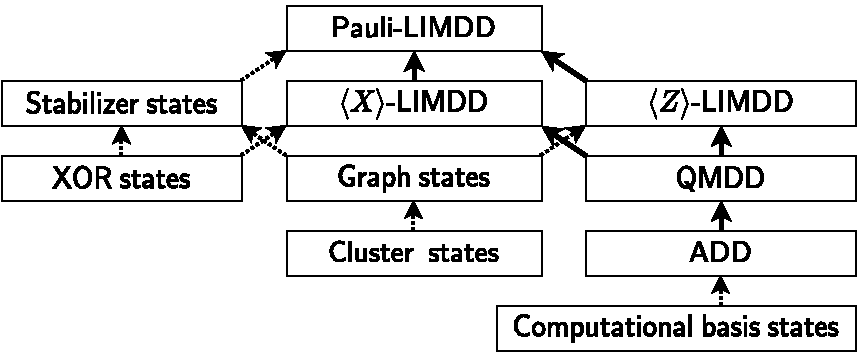
\includegraphics[width=0.55\textwidth]{pics/complexity-inclusion-diagram-no-torus.pdf}
	\caption{
	    \label{fig:complexity-classes-inclusion-diagram}
        Relations between classes of quantum states and families of polynomial-size decision diagrams.
        Every arrow denotes a strict inclusion of sets; in particular, each solid arrow $D_1\to D_2$ denotes an exponential separation between two decision diagram families, i.e., some quantum states have polynomial-size diagrams of type $D_2$, but have only exponential-size diagrams of type $D_1$. The dotted arrows represent inclusion.
%        \todo[inline]{remove DT}
    }
    %\vspace{-1em}
%    \end{centering}
\end{wrapfigure}

\autoref{fig:complexity-classes-inclusion-diagram} visualizes the results from this section.
The boxes with $\braket{Z}$-\limdd denote the \limdd with parameter \mbox{$G=\braket{Z}$}, i.e., \limdds where the labels on edges are all of the form \mbox{$\lambda P_n\otimes\cdots\otimes P_1$} where \mbox{$P_j\in \{\mathbb I, Z\}$}.
Although of course every $\braket{Z}$-\limdd is a Pauli-\limdd, this parameterization is interesting in its own right because it requires only polynomial size to represent any graph state.
Similarly, the $\braket{X}$-\limdd can succinctly represent a set of stabilizer states we call ``XOR states.''
\autoref{sec:graph-states-limdds} proves these results, and proves that \qmdds require exponential size for all these states. 
%Namely, we show that $\braket{Z}$-\limdds can represents graph states (\autoref{thm:z-limdd-is-graph-state}), and that $\braket{X}$-\limdds can represent so-called ``XOR-states'' (\autoref{thm:x-limdd-is-hyperplane}).




\begin{theorem}[Exponential separation between Pauli-\limdd versus QMDD union stabilizer states]
	\label{thm:limdd-superset-qmdd-plus-stabilizers}
	The set of quantum states represented by polynomial-size Pauli-\limdds is a strict superset of the union of stabilizer states and polynomial-size \qmdds.
\end{theorem}
\begin{proof}
    Each $n$-qubit stabilizer state can be represented by a Pauli-\limdd of $n$ nodes (\autoref{thm:pauli-limdd-is-stabilizer}).
    Moreover, if a state has a polynomial-size \qmdd, it also has a polynomial-size \limdd, due to our earlier remark that a \qmdd can be seen as a \glimdd with $G=\set{\mathbb I}$, i.e., each label is of the form $\lambda\mathbb I$ with $\lambda\in\mathbb C$.
%    This shows that the union of stabilizer states and polynomial-size QMDDs is included in the set of polynomial-sizee Pauli-\limdds.
    To show that polynomial-size Pauli-\limdds represent strictly more than these two classes of states, consider $\ket{\phi}:= \ket{T}\otimes \ket{G_n}$, where $\ket{T}=\ket{0}+e^{i\pi/4}\ket{1}$, and where $\ket{G_n}$ is the graph state on the $n\times n$ grid.
    We note that $\ket{\phi}$ is not a stabilizer state, because each computational-basis coefficient of a stabilizer state is of the form $z\cdot 1/\sqrt{2}^k$ for $z\in \{\pm 1, \pm i\}$ and some integer $k\geq 1$ \cite{nest2005local}, while $\bra{1}\otimes \bra{0}^{\otimes n} \ket{\phi} = e^{i\pi/4} \cdot \frac{1}{\sqrt{2}}^n$ is not of this form.
    Moreover, its canonical \qmdd is a root node $\lnode{1}{v_G}{e^{i\pi/4}}{v_G}$ where $v_G$ is the root node of the QMDD for $\ket{G_n}$, which has exponential size (\autoref{thm:graph-state-qmdd-lower-bound}).
    In contrast, the reduced Pauli-\limdd for $\ket{G_n}$ (with root node $w_G$) has $n$ nodes (because $\ket{G_n}$ is a stabilizer state), and hence a polynomial-size Pauli-\limdd for $\ket{T} \otimes \ket{G_n}$ has root node with $\lnode{\unit}{v_G}{e^{i\pi/4} \unit}{v_G}$.
\end{proof}


%In the following proofs, we  use a subset of \limdds, called Tower \limdds formalized in \autoref{def:tower}.
%\begin{definition}[Tower \glimdd]
%    \label{def:tower}
%	A \glimdd is called a Tower \glimdd if it has one node in each layer, i.e., if, for each node, both outgoing edges point to the same target (although these edges may have different labels).
%\end{definition}
%
%\autoref{thm:pauli-limdd-is-stabilizer} characterizes the Tower Pauli-\limdds.
%It is stated here informally; for details and a proof, see \autoref{sec:proof-stabilizer-states-tower-limdds}

Now we give the two statements leading up to \autoref{thm:limdd-superset-qmdd-plus-stabilizers}: \pauli-\limdds represent stabilizer states succinctly (\autoref{thm:pauli-limdd-is-stabilizer}) but \qmdds representing stabilizer states are necessarily large (\autoref{thm:graph-state-qmdd-lower-bound}).
In this theorem, by a Tower \limdd we mean a \limdd which has a single node on each level.

\begin{theorem}[Tower Pauli-\limdds are stabilizer states]
	\label{thm:pauli-limdd-is-stabilizer}
    Let $n>0$.
    Each $n$-qubit stabilizer state is represented by a reduced Tower Pauli-\limdd on $n$ nodes with high edge label factors $\in \{0, \pm 1, \pm i\}$.
	Conversely, every such \limdd represents a stabilizer state.
\end{theorem}
\begin{proof}[Proof sketch]
    We sketch here why each stabilizer state is represented by a reduced Tower Pauli-\limdd and give a full proof in \autoref{thm:pauli-tower-limdds-are-stabilizer-states}.
    Let $\ket{\psi}$ be a stabilizer state.
    If $\ket{\psi} = \ket{x}\ket{\psi'}$ for some $x\in \{0, 1\}$ and $\ket{\psi'}$, then $\ket{\psi'}$ is a stabilizer state and it is represented by a Tower Pauli-\limdd which has a root node with a low edge label $\id$, high edge label $0$ and root edge labelled $X^x \otimes \id$, to the root node of the Tower Pauli-\limdd of $\ket{\psi'}$.
	Otherwise, $\ket{\psi}\propto \ket{0}\ket{\psi_0}+\ket{1}\ket{\psi_1}$, where both $\ket{\psi_0}$ and $\ket{\psi_1}$ are stabilizer states.
    Moreover, if $\ket{\psi}$ is a stabilizer state, there is always a set of single-qubit Pauli gates $P_1,\ldots, P_n$ and a $\lambda \in \{\pm 1, \pm i\}$ such that $\ket{\psi_1}=\lambda P_n\otimes\cdots\otimes P_1\ket{\psi_0}$.
	That is, in our terminology, the states $\ket{\psi_0}$ and $\ket{\psi_1}$ are \emph{isomorphic}.
	Hence $\ket{\psi}$ can be written as
	\begin{align}
		\ket{\psi}=\ket{0}\ket{\psi_0} + \lambda \ket{1}\otimes \left(P_n\otimes\cdots\otimes P_1\ket{\psi_0}\right)
	\end{align}
	This expression suggests the following representation as a Tower Pauli-\limdd: the root node represents $\ket{\psi}$, both its outgoing edges point to a node representing $\ket{\psi_0}$, and its high edge is labeled with the isomorphism $\lambda P_n\otimes\cdots\otimes P_1$; this strategy is then applied recursively to $\ket{\psi_0}$ and its two subfunctions.
    This procedure yields a semi-reduced Tower-Pauli-\limdd, which can be made reduced by making all high labels canonical, from bottom to top.
\end{proof}

\begin{lemma}
	\label{thm:graph-state-qmdd-lower-bound}
	Denote by $\ket{G_n}$ the graph state on the $n \times n$ lattice.
	Each \qmdd representing the cluster state $\ket{G_n}$ has at least $2^{\floor{n/12}}$ nodes.
\end{lemma}
\begin{proof}[Proof sketch]
	Consider a partition of the vertices of the $n\times n$ lattice into two sets $S$ and $T$ of size $\frac{1}{2}n^2$, corresponding to the first $\frac{1}{2}n^2$ qubits under some variable order.
	Then there are at least $\lfloor n/3 \rfloor$ vertices in $S$ that are adjacent to a vertex in $T$ \cite[Th. 11]{lipton1979generalized}.
	Because the degree of the nodes is small, many vertices on this boundary influence the amplitude function independently of one another.
	From this independence, it follows that, for any variable order,
	the partial assignments $\vec a \in \set{0,1}^{\frac{1}{2}n^2}$ induce
	$2^{\lfloor n/12 \rfloor}$ different subfunctions $f_{\vec a}$, where
	$f\colon \set{0,1}^{n^2} \rightarrow \mathbb C$
	is the amplitude function of $\ket{G_n}$.
	The lemma follows by noting that a \qmdd has a single node per unique subfunction modulo phase.
	For details see \autoref{sec:graph-state-lower-bound}.
\end{proof}

%In \autoref{sec:proof-stabilizer-states-tower-limdds}, we characterize Tower $\braket{Z}$-\limdds (\autoref{thm:z-limdd-is-graph-state}) and Tower $\braket{X}$-\limdds (\autoref{thm:x-limdd-is-hyperplane}), and we give two more exponential separations (\autoref{thm:exponential-lower-bound-hyperplane} and \autoref{thm:exponential-separation-add-vs-qmdd}).
%Proofs of the characterizations appear in \autoref{sec:proof-stabilizer-states-tower-limdds}.

%\begin{theorem}[Tower $\braket{Z}$-\limdds are graph states]
%	\label{thm:z-limdd-is-graph-state}
%	For every graph state, there is a Tower-$\braket{Z}$-\limdd which represents that state.
%	Conversely, every Tower-$\braket{Z}$-\limdd represents some graph state.
%\end{theorem}
%
%\autoref{thm:x-limdd-is-hyperplane} talks about uniform superpositions.
%If $S\subseteq\{0,1\}^n$ is any set of $n$-bit vectors, then we are interested in the uniform superposition over the elements of $S$:
%\begin{align}
%	\ket{\chi_S}=\frac{1}{\sqrt{|S|}}\sum_{x\in S}\ket{x}
%\end{align}
%
%\begin{theorem}[Tower $\braket{X}$-\limdds are XOR-states]
%	\label{thm:x-limdd-is-hyperplane}
%	For every hyperplane $H\subseteq \{0,1\}^n$, there is a Tower-$\braket{X}$-\limdd which represents the state $\ket{\chi_H}$.
%	Conversely, every Tower-$\braket{X}$-\limdd represents the state $\ket{\chi_H}$ for some hyperplane $H$.
%\end{theorem}
%
%\begin{theorem}[X lower bound]
%	\label{thm:exponential-lower-bound-hyperplane}
%	\todo[inline]{To do: fetch this theorem from a previous version of the document -LV}
%\end{theorem}\todo{Why do we need this?}

Finally, we note an exponential separation between \qmdds and \adds.
Although we do believe this fact may be known in the decision diagram community, to the best of our knowledge this separation does not appear in the literature.

\begin{theorem}
	\label{thm:exponential-separation-add-vs-qmdd}
	There is an infinite family of quantum states $\{\ket{\phi_n}_n\}_{n}$ such that every \add needs $\Theta(2^n)$ nodes to store $\ket{\phi_n}$, but every \qmdd needs only $\Theta(n)$ nodes.
\end{theorem}
\begin{proof}
	The family of states is
	\begin{align*}
		\ket{\phi_n}=(\ket{0}+e^{i\pi}\ket{1})\otimes (\ket{0}+e^{i\pi2^{-1}}\ket{1})\otimes \cdots \otimes (\ket{0}+e^{i\pi2^{-n+1}}\ket{1}),
	\end{align*}
	which is a product state and can thus be represented by a \qmdd on $n$ nodes.
	In contrast, the computational-basis amplitudes are $\langle x |\phi_n\rangle = e^{i\pi x2^{-n}}/\sqrt{2^n}$ for $x \in \{0, 1, \dots, 2^n-1\}$ in binary notation, and therefore no two $\ket{x}$ share the same amplitude, resulting in $2^n$ leaves of the~\add.
\end{proof}


%\todo[inline]{The next section shows that LIMDDs not only represent a larger set of quantum states, but can also manipulate them efficiently, realizing a new method of simulation of quantum computing. In Section 6, we introduce some quantum circuits which LIMDDs can simulate efficiently, but which we suspect cannot be simulated with with existing simulators.}

%\input{sections/induced_subgraph_function.tex}
%\input{sections/X_iso_qmdd_lower_bound.tex}
%\subsection{Exponential separation of QMDD from ADD}

Algebraic Decision Diagrams (\textsf{ADD}) are a precursor to \textsf{QMDD}s.
The \textsf{QMDD} data structure groups together nodes representing subfunctions which differ only by a multiplicative constant.
By labelling the edges with appropriate weights, no information about the state is lost.
In this Section, we show that this leads to an exponential decrease in the size of the diagram.
Put another way, we have $\textsf{ADD}\subsetneq \textsf{QMDD}$.
In the literature, \textsf{ADD} is sometimes called \textsf{QuiDD}.

\begin{theorem}
	There is an infinite family of quantum states $\{\ket{\phi_n}_n\}_{n}$ such that every reduced, ordered \textsf{ADD} needs $\Theta(2^n)$ nodes to store $\ket{\phi_n}$, but every \textsf{QMDD} needs only $\Theta(n)$ nodes.
\end{theorem}
\begin{proof}
	The state is the Fourier-transformed state
	\begin{align}
		\ket{\phi_n}=(\ket{0}+e^{i\pi})\otimes (\ket{0}+e^{i\pi2^{-1}})\otimes \cdots \otimes (\ket{0}+e^{i\pi2^{-n+1}})
	\end{align}
	Since the state is a product state, its QMDD only has $n$ nodes, not counting the \textsf{leaf} node.
	
	However, the amplitudes of each basis vector is different, so the \textsf{ADD} has an exponential number of leaves, each containing a different amplitude. Namely, the amplitude in $\ket{\phi}_n$ of basis vector $\ket{x}_n$ is $\frac{1}{\sqrt{2^n}}e^{i\pi x2^{-n}}$.
\end{proof}
\section{Simulating Quantum Circuits with Pauli-\limdds}
\label{sec:quantum-simulation}

%\todo[inline]{
%-- Prune this overview, referring to Table 2.
%
%-- IMPORTANT: Invent a way to portray the complexities in Table 2 more fairly:\\
% Note that for states/circuits where
% LIMDDs/QMDDs take exponential time, so do ADD (because of their size)! The current caption is not sufficient!
% }

In this section, we give all the algorithms that are necessary to analyze and simulate a quantum circuit with Pauli-\limdds (we will simply say \limdd from now on).
We provide algorithms for dedicated gates, but also an algorithm to apply any multi-qubit gate that is represented as a \limdd.
We also give the subroutine \makeedge which is used to keep the diagram reduced throughout the computation, thus preventing the creation of redundant nodes, keeping the diagram small and canonical. The procedure is the counterpart of `MakeNode' used in other DD definitions for that purpose.
\autoref{tab:complexity} provides an overview of the \limdd algorithms and their 
complexities compared to ADDs and QMDDs (an unequal comparison due to the exponential differences in conciseness shown in \autoref{sec:exponential-separations}).

%In \autoref{sec:equality}, we give a polynomial-time algorithm which checks whether two given \limdds represent the same quantum state.
%In \autoref{sec:measurement}, we give a linear-time algorithm which simulates a measurement performed on the state represented by a \limdd.
%We show both how to compute the probability of observing a given measurement outcome, and how to update the \limdd after a given measurement.
%That is, given a \limdd representing a matrix $U$, and a \limdd representing a state $\ket{\phi}$, \autoref{alg:apply-gate-limdd-limdd} constructs a new \limdd representing the state $U\ket{\phi}$.
%For sake of exposition, we first describe how to apply certain simple gates such as Pauli gates and the Hadamard gate, in \autoref{sec:simple-gates}.
%Lastly, \autoref{sec:makeedge} describes the subroutine \makeedge which is used to keep the diagram reduced throughout the computation, thus preventing the creation of redundant nodes keeping the diagram small and canonical. The procedure is the counterpart of `MakeNode' used in other DD definitions for that purpose.

%\todo[inline]{fix Hadamard for stabilizers}

%\begin{wrapfigure}{r}{5cm}
%        \begin{tikzpicture}[
%        scale=0.3,
%        every path/.style={>=latex},
%        every node/.style={},
%        inner sep=0pt,
%        minimum size=0.5cm,
%        line width=1pt,
%        thin,
%        font=\small
%        ]
%
%        % nodes
%        \node[draw,circle] (a1) at ( 0,-0)     {$a_1$};
%        \node[draw,circle] (a2) at (0,-3) {$a_2$};
%
%        \node[draw,circle,rectangle,minimum size=0.4cm] (w1) at ( -0,-6) {$1$};
%
%        % edges
%        \draw[dotted,bend left=-20] (a1) edge  node[left] {$\alpha$} (a2);
%        \draw[bend left=20]        (a1) edge  node[right] {$\beta$} (a2);
%        
%        \draw[dotted,bend left=-20] (a2) edge node[left] {$a$} (w1);
%        \draw[bend left=20]       (a2) edge  node[right] {$b$} (w1);
%        
%        
%        \node[color=white,below = .2cm of w1] {$\approx$ AADD / SLDD / QMDD};
%    \end{tikzpicture}
%\end{wrapfigure}


%First, in \autoref{sec:measurement}, we give a linear-time (in the size of the \limdd) algorithm for performing a measurement.
%Then, in \autoref{sec:simulation}, we show how to apply a gate to a state, represented as \limdd.
%Then, \autoref{sec:pauli-isomorphism-detection} shows how to choose LIMs for diagram edges.
%
%The intended usage of the algorithms is to realize simulation of quantum computing and circuit optimization.
%For example, a typical simulator implementation starts with a single \limdd representing the quantum state $\ket{0}$ on $n$ qubits (this \limdd has $n$ nodes). Next, it builds a \limdd for each gate, using \autoref{def:limdd-as-matrix} explained below.
%Then, it applies these gates to the state one by one,
%each time obtaining a new \limdd which represents the intermediate quantum state.
%Finally, the probability of measurement outcomes can be computed using \autoref{alg:measurement-top-qubit}.


%Complexity of currently \emph{best-known algorithm} for applying specific operations
%            on input diagrams representing states $\ket \phi$ (and $\ket \psi$).
%            To account for the different representation sizes 
%            (see the exponential separations \add < \qmdd < \limdd given in \autoref{sec:exponential-separations}), we provide all complexities normalized to the \add size $m = \sizeof{D^\add_\phi}$
%            (and $m' = D^\add_\psi$).    

\begin{table}[hbt!]
    \caption{Complexity of currently \emph{best-known algorithm} for applying specific operations, in terms of the size of the input diagram size $m$
       (i.e., the number of nodes in the DD) and the number of qubits $n$.
    	Although addition of quantum states is not, strictly speaking, a quantum operation, we include it because it is a subroutine of gate application.
        Although the table seems to suggest that \add is faster than \qmdd and \limdd, we emphasize that \qmdd is never slower than \add, and \limdd is never slower than \qmdd modulo a multiplicative factor $O(n^3)$ due to calls to \textsc{MakeEdge}.
    	The discrepancy appears because runtime is given as a function of decision diagram size, and \adds / \qmdds are sometimes exponentially larger than \limdds (see \autoref{sec:exponential-separations}).
       Note that several of the \limdd algorithms invoke \textsc{MakeEdge}
            and therefore inherit its cubic complexity (as a factor).
%            \todo[inline]{Vedran: maybe just say in words that of course it is not an issue that LIMDD loses, because $D_Q$ and $D_A$ will be exponentially larger than. $D_L$ for some states and circuits...}
%    \todo[inline]{Vedran:I don't really ... aha you need to have separate sizes as there is a non trivial interplay betwen n and these quantities?  It may look like comparing apples and oranges (DA DL DQ)}
        }
\label{tab:complexity}
\begin{tabular}{c|lll|r}
    \bf Operation $\backslash$ input: &\bf \add
                    & \bf \qmdd & \bf \limdd & \bf Section \\
\hline
Checking state equality &  $\oh(1)$ & $\oh(1)$ & $\oh(n^3)$ & \autoref{sec:equality} \\
    Single $\ket{0}/\ket{1}$-basis measurement &  $\oh(m)$ & $\oh(m)$ & $\oh(m)$ & \autoref{sec:measurement} \\
Single Pauli gate  &  $\oh(n)$ & $\oh(n)$ & $\oh(1)$ & \autoref{sec:simple-gates} \\
Single Hadamard gate / \textsc{Add()}  &  $\oh(m^2)$ & $\oh(2^n)$ note\footnote{Only exponential when the \add representing the same state is already large, i.e., $\sizeof{\add}\in \Omega(2^n)$. See for details \autoref{fig:explosion} and \cite[Table~2]{fargier2014knowledge}. \label{fn1}}  & $\oh(n^3 2^n)$ note$^{\ref{fn1}}$ & \autoref{sec:simple-gates} \\
Clifford gate on stabilizer state & $\oh(2^n)$ & $\oh(2^n)$ & $\oh(n^4)$ & \autoref{sec:simple-gates} \\
%&   \multicolumn{3}{c|}{\footnotesize (exponential only if $\sizeof{D_A} \in \oh(2^n)$!)
%    %if \limdd / \qmdd takes exp. time then $\sizeof{D_A}\in \oh(2^n)$
%} & \\
Multi-qubit gate  & $\oh(4^n)$ note\footnote{The \NP-complete satisfiability problem can be reduced to matrix vector multiplication in (poly-sized) BDDs~\cite{mcmillan}.
In practice however, this rarely poses a problem~\cite{chaki2018bdd}. \label{fn2}}
     & $\oh(4^n)$  note$^{\ref{fn2}}$  & $\oh(n^34^n)$  note$^{\ref{fn2}}$  & \autoref{sec:simulation} \\
%Addition & $\oh(m_1m_2)$ & $\oh(2^n)$ & $\oh(n^32^n)$ & \autoref{sec:simulation}\\
MakeNode / \makeedge (\limdd) &  $\oh(1)$ & $\oh(1)$ & $\oh(n^3)$ & \autoref{sec:makeedge} 
\end{tabular}
\end{table}

%\todo[inline]{``\limdd is never slower than \qmdd'': except for cubic factor?}


Our algorithms will use the notation in \autoref{tab:notation} to easily navigate and construct diagrams.
The notation $\ledge Av$ creates an edge to an existing node $v$, labeled with a LIM $A$.
%The dot notation, e.g., $\ledge Av$, allows (root) edge construction to node $v$ with LIM $A$.
If $v_0$ and $v_1$ are two existing nodes, then the notation $\lnode A{v_0}B{v_1}$ creates a new (not-necessarily-reduced) node
whose left edge is $\ledge A{v_0}$ and whose right edge is $\ledge B{v_1}$.
%The $\plus$ notation combines edges $\ledge A{v_0}$ and $\ledge B{v_1}$ into a node with low ($v_0$) and high child ($v_1$).
LIMs are decomposed using  $A = \lambda_A  P_n \otimes P' $.
%We will often write a LIM as $A=\lambda P_n\otimes\cdots\otimes P_1$.
Here $\lambda_A\in \mathbb C$ is a non-zero scalar, and the matrices satisfy $P_j\in \set{\mathbb I,X,Z, Y}$ for every $j$.
Finally, the \follow b{\ledge {\lambda P_n\otimes P'}v} notation allows us to \emph{semantically} follow low and high edges, by applying $P_n$ on qubit $\index(v)=n$ and returning either $\low v$ or $\high v$
multiplied by $\lambda_A P'$.
Specifically, if $e$ is an edge with $\ket{e}=\ket{0}\ket{\phi_0} + \ket 1\ket{\phi_1}$, then $\follow be$ denotes an edge $f$ satisfying $\ket{f}=\ket{\phi_b}$.
The amplitude of basis state $\ket{1111}$ for the \limdd root edge $e$ in \autoref{fig:qmdd-isoqmdd-exposition} is computed by taking $\ket{\follow {1111}{e}} = \ket{\ledge{\omega e^{\frac\pi4 i}}{1}} = \omega e^{\frac\pi4 i}$.


\begin{table}[h]\def\arraystretch{1.4}
\caption{Notation to navigate and construct \limdds.}
\label{tab:notation}
\begin{tabular}{|l|l|l|}
\hline
\bf Type & \bf Notation & \bf Semantics \\ %& \bf Figure \\
\hline
(New) \Edge $e$
    & $\ledge[e] Av$  &  $ \ket e = \ket{\ledge Av} \defn A \ket{v}$ 
     \\
\hline
(New) \Node $v$
    & $\lnode[v]{A}{v_0}{B}{v_1}$ & $\ket{ v} \defn \ket 0 A\ket{v_0} + \ket 1 B\ket{v_1}$
      \\
\hline
$\Node \to \Edge$
    & $B \cdot v$  &
        $\defn  \ledge {B}v $
  \\
$\Edge \to \Edge$
    & $B \cdot (\ledge Av)$  &
        $\defn  \ledge {B A}v $
  \\
\hline
$\Edge \to \Edge$
    & $\follow b{\ledge {\lambda X^x \begin{smallmat}z_1 & 0 \\ 0 & z_2  \end{smallmat} \otimes P' }v}$  & 
    $\defn   \begin{cases}
        \ledge {z_1\lambda  P' B_0}{v_0}   & \textbf{if } x = b,  ~\low v = \ledge{B_0}{v_0}\\
         \ledge {z_2\lambda  P' B_1}{v_1}  & \textbf{if } x \neq b,  \high v = \ledge{B_1}{v_1}\\    
        \end{cases}$
  \\ 
\hline
$\Edge\to \Edge$
    & $\follow {b_n\dots b_1}{\ledge Av}$  &
        $\defn \follow {b_1}{ \dots \follow {b_N}{\ledge Av}.. }$
   \\
\hline
\end{tabular}
\end{table}

%\todo[inline]{\follow{}{} does not return a quantum state! $\propto$ is still in the figure!}

%	\raisebox{-1mm}{\scalebox{.7}{\tikz{
%		\node[state,minimum size=.2cm] (1) {$v$};
%		\node (-a1) [above left  =.1cm and .3cm of 1] {};
%		\node (-b1) [above right  =.1cm and .3cm of 1] {};
%		\node (1a-) [below left =.1cm and .3cm of 1] {};
%		\node (1b-) [below right = .1cm and .3cm of 1] {};
%		
%		\path[]
%		(-a1) edge node {} (1)
%		(-b1) edge node {} (1)
%		(1) edge node {} (1a-)
%		(1) edge node {} (1b-);
%	}}}.



%
%\begin{itemize}
%    \item We write $\Edge(v, A, w)$ for an edge $e = (v,w)$ with $\lbl(e) = A$ and
%        $\Edge(A, v)$ for a root edge (without source).
%        \item We write $e_0^v=(v,\label(\low(v)),\low(v))$ and $e_1^v=(v,\label(\high v),\high v)$ to indicate the low and high edges out of node $v$, respectively. Note that this allows us to write $e_x^v$ for $x\in\{0,1\}$.
%        \item We write $\textsc{Node}(v_0,v_1,A)$ for a \emph{low-factored} node $v$ with low child $v_0$, high child $v_1$, its low edge labeled with $\mathbb I^{\otimes \index(v_0)}$ and its high edge labeled with $A$.
%    \item The LIMs of edges $e=(v, w)$ can be manipulated using multiplication, e.g.,: 
%            $\lambda A \cdot e$ yields an edge $e'$ with $\lbl(e')= \lambda A \cdot \lbl(e)$
%            for any LIM $A = A_{\index(w)} \otimes \dots \otimes A_1 $. 
%    \item An edge $e=(\cdot, A' \otimes \diag{z}, v)$ can be followed `semantically,' by pushing the LIMs down the DD: $e_{\downarrow 0}$ ($e_{\downarrow 1}$) represents the edge $A' \cdot \low(v)$  ($z A \cdot \high v$). When $e=(\cdot, A' \otimes \anti{z}, v)$ then: $e_{\downarrow 0}$ ($e_{\downarrow 1}$) represents the edge $z A' \cdot \high v$  ($ A \cdot \low(v)$).
%\end{itemize}






%\todo[inline]{The text below can be improved. -LV Be inspired by: https://link.springer.com/content/pdf/10.1023/A:1008647823331.pdf}

All \limdd operations discussed in this section return reduced \limdds by creating edges and nodes using a dedicated \makeedge operation.
The complexity of computing LIMs to find a canonical representative for each isomorphism equivalence class resides in this function. We will therefore defer the treatment of this function to the end of this section. For now, the reader can assume a trivial (non-reducing) implementation of the functions as given in \autoref{alg:make-edge-prov}. Like other DD structures, \limdds require a unique table (a set) to uniquely store canonical representatives.

\begin{algorithm}
	\begin{algorithmic}[1]
		\Procedure{\makeedge}{\Edge $\ledge {A}{v}$, \Edge $\ledge Bw$}
			\State  \Return $\lnode AvBw$
		\EndProcedure
	\end{algorithmic}
	\caption{Provisionary algorithm \makeedge for creating nodes modulo reduction.}
	\label{alg:make-edge-prov}
\end{algorithm}

In line with other existing efficient decision-diagram algorithms, we use dynamic programming in our algorithms to avoid traversing all paths  (possibly exponentially many) in the \limdd (DAG).
To implement this, we use a cache data structure (a lossy set) storing the parameters of the recursive function calls.
%Doing so avoids re-evaluating our algorithms on inputs that were encountered earlier.
%We will explicitly mention when the resulting algorithms run in polynomial time
%in the number of nodes of the input \limdds.\todo{why? We should clarify all complexities stated in Table 2.}


%\todo[inline]{Necessary, but sufficient for universal? Perhaps give a bottom line or refer to Section 5?}

%In this Section, we sketch algorithms for manipulating \limdds.
%In particular, for updating a \limdd after a applying a gate or computational-basis measurement and for reducing the size of a \limdd by identifying isomorphic nodes.
%


\subsection{Checking state equality}
\label{sec:equality}

Contrary to other decision diagrams, the nodes of a \limdd do not represent a single quantum state but an entire equivalence class of states (see \autoref{cor:node-canonicity-strong}). While reduced nodes are canonical descriptions of these equivalence classes, only the root edge, representing individual quantum states in an equivalence class, is not necessarily canonical.

Given two \limdds representing the states $\ket{\phi}$ and $\ket{\psi}$, we can check in $\oh(n^3)$ time whether $\ket{\phi}=\ket{\psi}$ using \autoref{alg:equality-check}.
The algorithm uses the canonicity of \limdds, which guarantees that two reduced nodes represent the same state if and only if they are equal, and which guarantees that no two nodes represent isomorphic states (\autoref{cor:node-canonicity-strong}).
We have $A\ket{v}=B\ket{w}$ if and only if $\ket{v}=A^{-1}B\ket{w}$, which, due to canonicity, can only hold if $A^{-1}B\ket{w}=\ket{w}$.
That is, $A^{-1} B$ is a \emph{stabilizer} of $\ket{w}$ and $A^{-1}B$ is an element of the stabilizer subgroup of $\ket{w}$ (see \autoref{sec:preliminaries}).
We check whether $A^{-1}B$ is a stabilizer of $\ket{w}$ in two steps, assuming we have computed generators for the stabilizer subgroup of $\ket{w}$ (see \autoref{sec:pauli-isomorphism-detection}): first, we check if $A^{-1}B$ commutes with all stabilizer generators. If not, then $A^{-1}B$ cannot be a stabilizer of $\ket{w}$.
If it does, then either $A^{-1}B$ or $-A^{-1}B$ is a stabilizer of $\ket{w}$.
To distinguish these two cases, we use the Membership algorithm of \autoref{sec:preliminaries} while keeping track of the scalars.
The complexity of \autoref{alg:equality-check} is in $\oh(n^2)$ time.
In \autoref{sec:makeedge} we will introduce algorithms for stabilizers more completely.

\begin{algorithm}
	\caption{Checks whether two reduced \limdds represent the same state. The input is the two root edges, pointing to the root nodes $v$ and $w$ of the two diagrams.}
	\label{alg:equality-check}
	\begin{algorithmic}[1]
		\Procedure{Equality-check}{\Edge $\ledge Av$, \Edge $\ledge Bw$ \textbf{with} reduced $v,w$}
%			\State \textbf{precondition:} nodes $v$ and $w$ are reduced according to \autoref{def:reduced-limdd}
			\State 
            \Return  $v=w  $ \textbf{and}  ($A = B = 0$ \textbf{or} $A^{-1}B\in \Stab(v)$)
		\EndProcedure
	\end{algorithmic}
\end{algorithm}


\subsection{Performing a measurement in the computational basis}
\label{sec:measurement}
\defmath{\project}{\textsc{UpdatePostMeas}}

We provide a subroutine that, given a \limdd representation of a state, can sample the outcome of computational-basis measurements on the state (i.e., weak simulation), and a subroutine to compute the exact probability of measuring a given computational basis state $\ket{x}$ for $x\in \{0,1\}^n$ (i.e., strong simulation).
For brevity, we do so only for the top qubit. The general case is described in \autoref{sec:advanced-algorithms}.


Simulating the computational-basis measurement of the top qubit of an $n$-qubit \limdd, as part of a larger quantum state $\ket{\phi} = \ket{0} \ket{\phi_0} + \ket{1} \ket{\phi_1}$, consists of two parts: first, obtaining the probability of observing output $m\in\{0, 1\}$, which equals 
\[
    p(m) = \bra{\phi} \left(\dyad{m} \otimes \id[2]^{\otimes (n-1)}\right) \ket{\phi}/\braket{\phi|\phi} = \langle \phi_m | \phi_m \rangle / \langle \phi | \phi \rangle.
\]
This allows one to to determine which outcome is observed by throwing a random $p(0)$-biased coin.
Second, updating the \limdd to the (here unnormalized) post-measurement state $\left(\ket{m}\bra{m} \otimes \id[2]^{\otimes (n-1)}\right) \ket{\phi} = \ket{\phi_m}$ after obtaining outcome $m$.
In \autoref{alg:measurement-top-qubit}, we provide efficient algorithms for both parts in case the measured qubit is the top qubit of a \limdd.

The runtime of computing the probability of a measurement outcome is dominated by the runtime of the subroutine \textsc{SquaredNorm}, which computes the quantity $|\braket{e|e}|$ given a \limdd edge $e$.
By saving the squared norm of each node in cache, the algorithm only needs to visit each node once.
Consequently, this algorithm runs in time $\oh(m)$ when the diagram has $m$ nodes.


The \project algorithm is straightforward: in order to update the state $\ket{e}=\ket 0\ket{e_0} + \ket 1\ket{e_1}$ after the top qubit is measured to be $m$, we simply construct an edge $\ket{m}\ket{e_m}$ using the \makeedge subroutine.
The runtime is $\mathcal O(n)$, since in this case \makeedge only needs to find a new label for the root edge.


\begin{algorithm}[h]
	\begin{algorithmic}[1]
		\Procedure{MeasurementProbability}{\Edge $\ledge Av$ \textbf{with} $A=\lambda P_n \otimes  \dots \otimes P_1$}
%		\State (Say that $A=X^{x}\diagonal{z}\otimes A^\prime$ for some $x\in \{0,1\}$ and $z\in S(1)$.)
		\State $p_0 := \textsc{SquaredNorm}(\low v)$
		\State $p_1 := \textsc{SquaredNorm}(\high v)$
		\State \Return $p_i/(p_0+p_1)$ \textbf{for} $i = (P_n \in \set{X, Y})$  \Comment{(anti-)diagonal \pauli{}s}
%		\State \textbf{if} $P_n \in \set{X, Y}$ \textbf{then} \Return $p_1/(p_0+p_1)$ \Comment{anti-diagonal \pauli{}s}
		\EndProcedure
        \Procedure{SquaredNorm}{$\Edge \ledge{\lambda P}{v}$}
		\If{$n=0$}
%	\State 
		\Return $|\lambda|^2$
%		\Else
		\EndIf
		\If{$v\in \textsc{cache}$}
		 \Return $|\lambda|^2\cdot \textsc{cache}[v]$ \Comment{Dynamic programming}
		\EndIf
		\State $s:= \textsc{Add}(\textsc{SquaredNorm}(\follow 0{\ledge {\mathbb I}v}),\textsc{SquaredNorm}(\follow 1{\ledge {\mathbb I}v}))$
		\State $\textsc{cache}[v]:=s$ \Comment{Store in dynamic programming cache}
		\State \Return $|\lambda|^2s$
		\EndProcedure
        \Procedure{\project}{\Edge $\ledge[e]{\lambda P_n \otimes P'\hspace{-2mm}}{v}$, measurement outcome $m\in\set{0,1}$}
        \If{$m=0$}
	        \State \Return $\makeedge(\follow 0e, ~~0 \cdot \follow 0e)$
        \Else
	        \State \Return $\makeedge(0 \cdot \follow 1e,~~ \follow 1e)$
        \label{l:project-diag}
            \EndIf
				  \label{l:project-project}
%		 \State \Return $e$
		\EndProcedure
	\end{algorithmic}
    \caption{Algorithms \textsc{MeasurementProbability} and \textsc{\project} for respectively computes the probability of observing outcome $0$ when measuring the first qubit of a Pauli \limdd in the computational basis and converting the \limdd to the post-measurement state after outcome $m\in \{0, 1\}$.
		The subroutine \textsc{SquaredNorm} takes as input a Pauli \limdd edge $e$, and returns $\braket{e|e}$.}
	\label{alg:measurement-top-qubit}
\end{algorithm}


To sample a bitstring as measurement outcome, simply repeat the measurement procedure outlined above $n$ times, i.e., first compute the probability $p$ of observing a $1$ for the top qubit, and then throw a $p$-biased coin, obtaining outcome $m$, and lastly update the \limdd according to the outcome, and repeat this process for the second qubit, then the third, etc.

For strong simulation, given a bit-string $x=x_n\ldots x_1$, first compute the probability $p_n$ of observing $x_n$; then update the \limdd to outcome $x_n$, obtaining a new, smaller \limdd.
On this new \limdd, compute the probability $p_{n-1}$ of observing $x_{n-1}$, and so forth.
Note that $p_{n-1}$ is the probability of observing $x_{n-1}$ given that the top qubit is measured to be $x_n$.
Then the probability of observing the string $x$ is the product $p=p_1\cdots p_n$.




\subsection{Simple Gates}
\label{sec:simple-gates}
Before we give the algorithm for arbitrary gates in \autoref{sec:simulation}, we first show how to apply several simple gates, most of which efficiently.
\autoref{fig:gates-examples} illustrates some of these gates.
In the description below, for brevity we omit the calls to \makeedge to make the diagram canonical again.
\begin{itemize}
    \item Applying a \textbf{single-qubit Pauli gate} $Q$ to qubit $k$ of a \limdd can be done in constant time, by updating the diagram's root edge from $\lambda P_n\otimes\cdots\otimes P_1$ to $\lambda P_n\otimes\cdots\otimes P_{k+1}\otimes QP_k\otimes P_{k-1}\otimes\cdots\otimes P_1$.
    \item Applying the \textbf{S gate} $\begin{smallmat}1& 0\\ 0& i\end{smallmat}$ to qubit with index $k$ is also efficient.
            If $k=n$ (top qubit), then note $S \rootlim \ket{v_{\textnormal{root}}} = (S \rootlim S^{\dagger}) S \ket{v_{\textnormal{root}}}$ where $S \rootlim S^{\dagger}$ is an ($O(n)$-computable) Pauli LIM because $S$ is a Clifford gate.
            Further, applying $S$ to $v_{\textnormal{root}}$ yields a multiplication with $i$ of the high edge.
            If $k<n$, then we note $S_k(\ket{0} \otimes \ket{v_0} + \ket{1} \otimes \highlim \ket{v_1}) = (\ket{0} \otimes S_k\ket{v_0} + \ket{1} \otimes \left(S_k\highlim S_k^{\dagger}\right) S_k \ket{v_1})$, where, again $S_k \highlim S_k^{\dagger}$ is a Pauli LIM.
        \item The application of a \textbf{downward Controlled-Pauli gate} $CQ_{t}^c$ ($Q$ is a single-qubit Pauli gate, $c$ is the control qubit, $t$ is the target qubit with $t<c$) is similar to the $S$ gate in case $c$ is not the top qubit, since controlled-Pauli gates are Clifford gates.
            If $CQ_{t}^c$ is applied to node $v$ with $\index(v)=c$, then update $v$'s high edge label as $\highlim \mapsto Q_t \highlim$.
    This operation takes $\oh(m)$ time on a diagram with $m$ nodes. A similar algorithm exists for the application of a \textbf{downward Controlled-Pauli string}.
\item To apply a \textbf{Hadamard gate} to the first qubit, see \autoref{alg:apply-hadamard}.
    The algorithm first constructs $\ket{a_0}=\ket{\phi_0}+\ket{\phi_1}$ and $\ket{a_1}=\ket{\phi_0} - \ket{\phi_1}$, and then constructs $H\otimes \mathbb I\ket{\phi} \propto \ket 0\ket{a_0} + \ket 1\ket{a_1}$.
    For \qmdds, it was known that applying a Hadamard gate ($H=\begin{smallmat}1 & 1 \\ 1 & -1\end{smallmat}$) to the top qubit of a state requires exponential time, because of the needed point-wise addition \cite[Table~2]{fargier2014knowledge}. However, this only happens, in cases where the \add version of the diagram is already exponential (otherwise addition for \adds would not be poly-time, which it is~\cite[Table~2]{fargier2014knowledge}).
    This behavior remains for \limdds, however \limdds can be exponentially more succinct than \qmdds as shown in \autoref{sec:exponential-separations}.
    Applying a Hadamard gate to a stabilizer state, represented as a \limdd, can be done in polynomial time, by \autoref{thm:hadamard-stabilizer-polytime} in \autoref{sec:hadamard-stabilizer-polytime}, which shows that the specific pointwise additions required to implement Hadamard are all $\oh(n^4)$.
\item Applying a \textbf{upward Controlled NOT}, i.e., $CX_t^c$ with $t>c$, can be done in polynomial time using only Hadamards and a downward CNOT because $CX_t^c = (H\otimes H) CX_c^t (H\otimes H)$.
\end{itemize}

It follows that applying Clifford gates to stabilizer states can be done in polynomial time.
In general, all Clifford gates are polynomial-time, except for the Hadamard gate.

\begin{algorithm}
	\caption{Applies a Hadamard gate to the first qubit. Specifically, given a \limdd edge for a state $\ket{\phi}$, returns a \limdd edge for the state $\ket{\psi}=H\otimes \unit_2^{\otimes n-1}\ket{\phi}$. \textsc{Add} is explained in \autoref{sec:simulation}.}
	\label{alg:apply-hadamard}
	\begin{algorithmic}[1]
		\Procedure{ApplyHadamard}{\Edge $\ledge[e] Av$}
			\State \Edge $a_0:=\textsc{Add}(\follow{0}{e},\follow{1}{e})$
			\State \Edge $a_1:=\textsc{Add}(\follow{0}{e},-\follow{1}{e})$
			\State \Return $\frac{1}{\sqrt 2}\cdot \makeedge(a_0,a_1)$
		\EndProcedure
	\end{algorithmic}
\end{algorithm}

\subsection{Applying a generic multi-qubit gate to a state}
\label{sec:simulation}

In order tot represent quantum gates ($2^n\times 2^n$ unitary matrices) using decision diagrams, we use the standard approach \cite{fujita1997multi}.
A natural choice is to let the coefficient of $\ket{a_1, \dots, a_n, b_1, \dots, b_n}$, for $a_j, b_j \in \{0, 1\}$ be the matrix entry in row $a$ and column $b$.
%In the vector interpretation, a \limdd can be seen as a (pseudo-Boolean) function $f(a_1, \dots, a_n) \in \complex$ with $a_i\in \bool$.
%Here $a_1,\ldots, a_n$ is the bitwise representation of $a$, so $f$ maps an index $0\leq a<2^n$ to the vector's value at that index.
%In the matrix interpretation, a \limdd is seen as a (pseudo-Boolean) function $m(a_1, \dots, a_n, b_1, \dots, b_n) \in \complex$  with $a_i,b_i\in \bool$, i.e., $m$ maps a pair of indices $a,b$ to the value of the matrix in row $a$ and column $b$.
%So the value $m(a,b)$ represents a single entry in the matrix.
% with $a_1, \dots, a_n, b_1, \dots, b_n$ the bitwise representation of $a, b$.
We slightly adjust this and interleave the row and column variables to facilitate recursive descent on the structure:
 $u(a_1, b_1, a_2, b_2,  \dots, a_n, b_n)$. Therefore, for $x,y\in \{0, 1\}$, the subfunction $u_{xy}$ represents a quadrant of the matrix, namely the submatrix
$u_{xy}(a_2, b_2,  \dots, a_n, b_n) \defn u(x, y, a_2, b_2,  \dots, a_n, b_n) $, as follows:
$
u=\overbrace{
\left.
\begin{bmatrix}
u_{00} &  u_{01}   \\    % NOTE removed colours because this led to typesetting fails sometimes
~u_{10} & u_{11} \\
\end{bmatrix}
\right\rbrace
}^{u_{0*}}
u_{* 1}
$.
\autoref{def:limdd-as-matrix} formalizes this.
\autoref{fig:gates-examples} shows a few examples of gates represented as \limdds.

\begin{definition}[\limdd{}s for gates]
	\label{def:limdd-as-matrix}
A reduced \limdd edge $\ledge Au$ can represent a (unitary) $2^n\times 2^n$ matrix $M$
iff $\index(u)=2n$.
The matrix value of cell $M_{r,c}$ is defined as $\follow{r_1 c_1 r_2 c_2 \dots r_n c_n}{\ledge Au}$
where $r,c$ are the row and column indices, respectively, with binary representation $r_1,\dots,r_n$ and $c_1,\dots,c_n$.
The semantics of a \limdd edge $u$ as a matrix is denoted $[u]\defn M$ (as opposed to its semantics $\ket{u}$ as a vector).
\end{definition}
\begin{figure}
	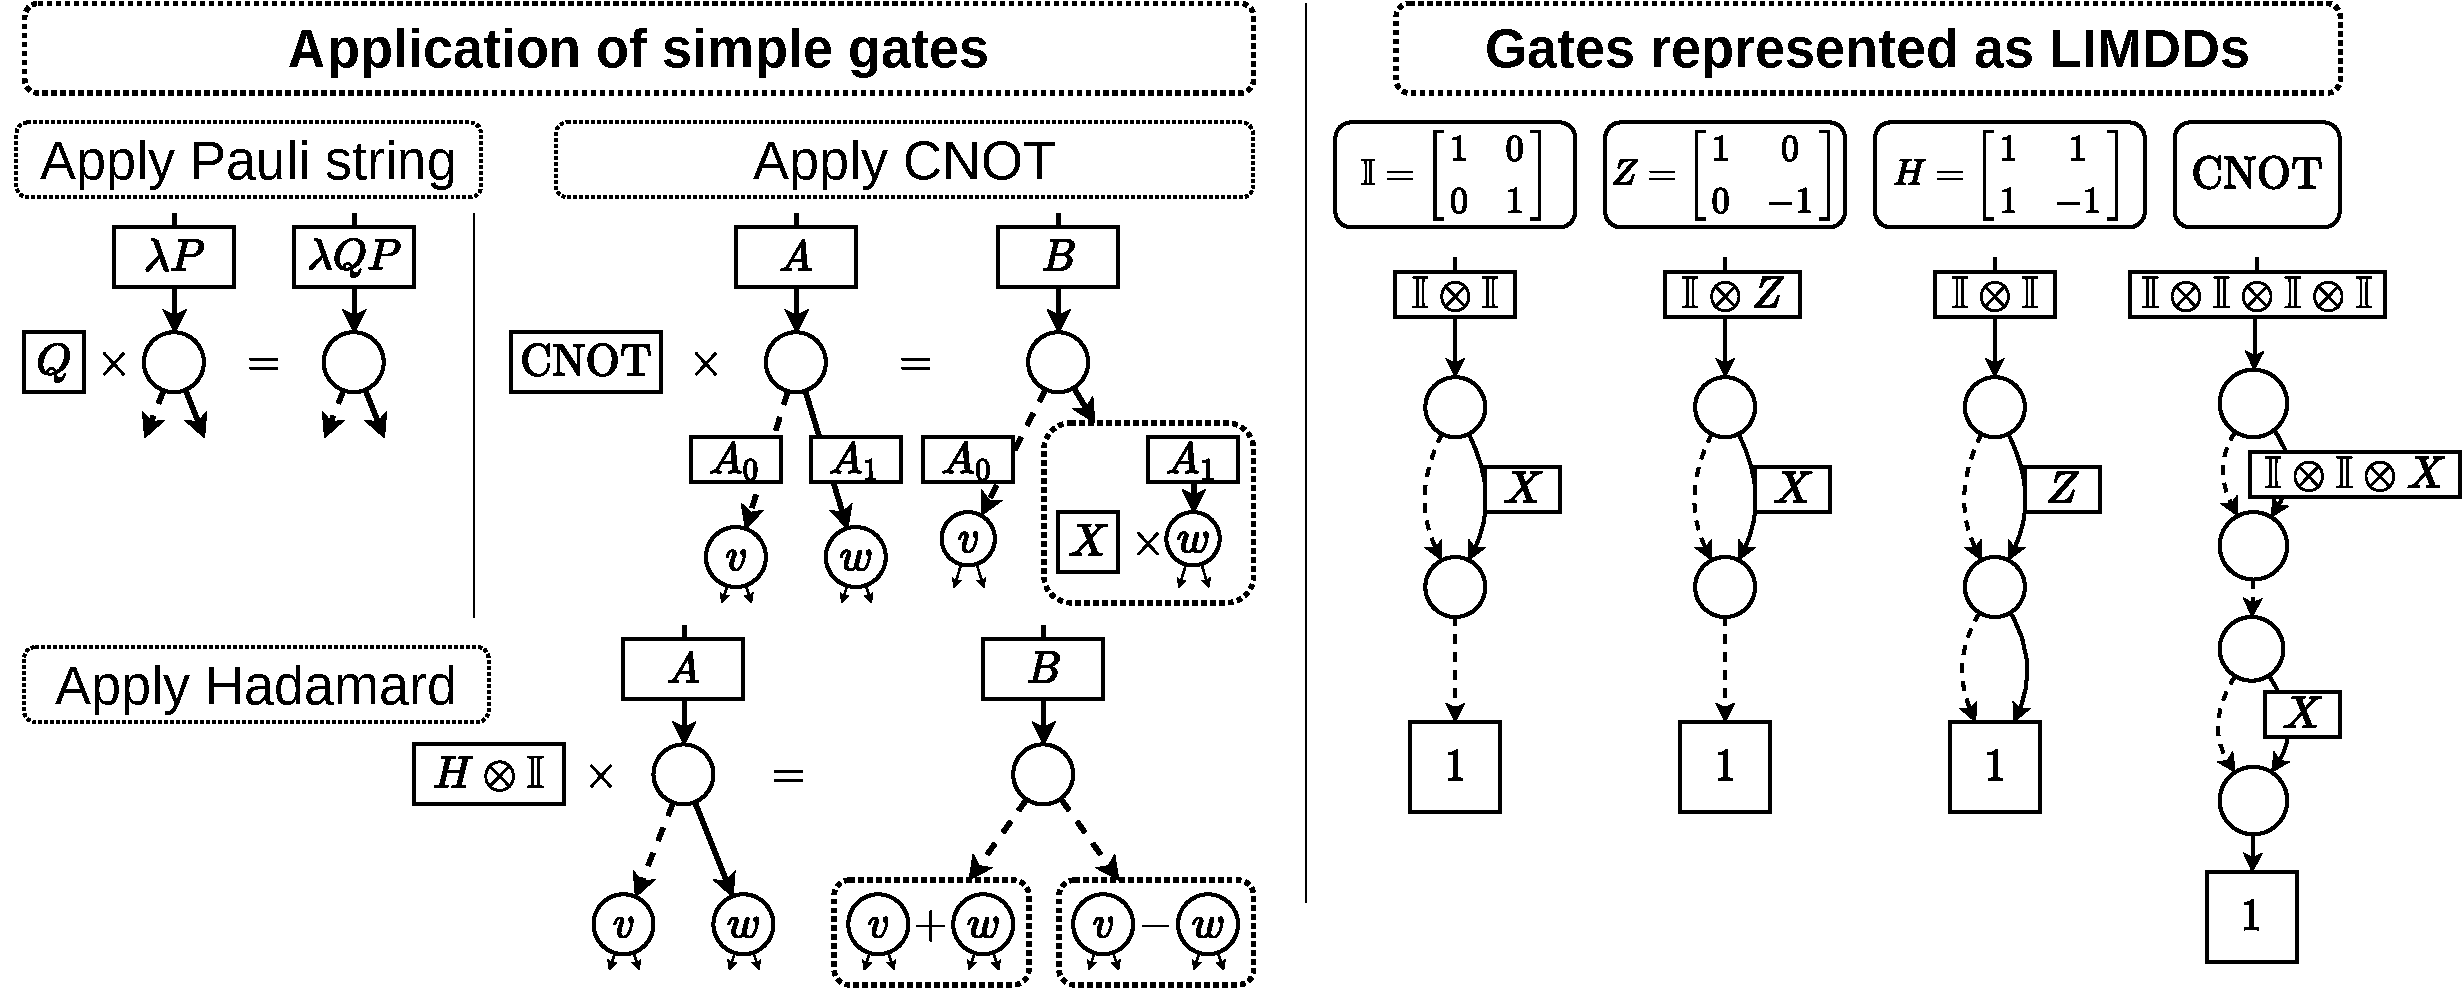
\includegraphics[width=\textwidth]{pics/gates-examples.pdf}
	\caption{\textbf{Left half}: illustration of applying several simple gates (some details are omitted).
		Leftmost: applying a Pauli string $Q$ to an edge entails only updating the label on that edge.
		Right: To apply a CNOT gate to the top qubit, apply $X\otimes \mathbb I^{\otimes n-2}$ to the right child; here this operation is represented inside a dotted box. The incoming edge's label changes from $A$ to $B=\text{CNOT}\cdot A\cdot\text{CNOT}$, which is guaranteed to be a Pauli string.
		Bottom: Applying a Hadamard gate on the top qubit is done by first making nodes representing $\ket{v}+\ket{w}$ and $\ket{v}-\ket{w}$, here shown in dotted boxes.
		\textbf{Right half}: Examples of four gates, represented as \limdds. Left: The identity gate $\mathbb I$ is represented by a \limdd of two levels. The first level indicates the row, and the second level indicates the column.
	Second from the right: the Hadamard gate; notice that the $Z$ label produces the $-1$ value in the matrix' bottom right entry.
	Rightmost: The CNOT gate. Since this gate is on $n=2$ qubits, it has $2n=4$ levels.
	Edges with label $\mathbb I$ are drawn without label; edges with label $0$ are not drawn.
	}
	\label{fig:gates-examples}
\end{figure}


%Here, we sketch algorithms for simulating quantum circuits using \limdds.
%In particular, \autoref{alg:apply-gate} shows how to apply a gate $\ket U$ to a state $\ket v$, where both  are represented as \limdds with root nodes $u$  and $v$.
%This recursive algorithm outputs (an edge to) a reduced \limdd $e$, representing $\ket{e}=U\ket{v}$.
%This edge is made on line \ref{algline:apply-gate-make-edge} with a call to \makeedge.
%This subroutine guarantees that the edge, and all nodes below it, satisfy all the reduction rules of \autoref{def:reduced-limdd}, making the result canonical.
%Consequently, all intermediate \limdds that are produced by the algorithm are reduced.

The procedure \textsc{ApplyGate} (\autoref{alg:apply-gate-limdd-limdd}) applies a gate $U$ to a state $\ket{\phi}$, represented by \limdds $e^u$ and $e^v$.
It outputs is a \limdd edge representing $U\ket{\phi}$.
%\autoref{alg:apply-gate} gives the procedure \textsc{ApplyGate} for updating a \limdd after applying an arbitrary gate $U$ to state $\ket \phi$ represented by \limdd edges $e^u$ and $e^v$.
%If we ignore the complexity\todo{we claim we can apply arbitrary gates, so we should do so or make clear immediately that we can.} 
%introduced by the labels on the edges $e^v$ and $e^U$\todo{$u$}, then the algorithm is quite straightforward:
It works as follows (see \autoref{fig:apply-gate} for an illustration).
Using the $\follow{x}{e}$ procedure, we write $\ket{\phi}$ and $U$ as
\begin{align}
	\ket{\phi} = & \ket{0}\ket{\phi_0}+\ket{1}\ket{\phi_1} \\
	U = & \ket{0}\bra{0}\otimes U_{00} + \ket{0}\bra{1}\otimes U_{01} + \ket{1}\bra{0}\otimes U_{10} + \ket{1}\bra{1}\otimes U_{11}
\end{align}
Then, on line \ref{algline:apply-gate-compute-term}, we compute each of the four terms $U_{rc}\ket{\phi_c}$ for row/column bits $r,c \in \{0,1\}$.
We do this by constructing four \limdds $f_{r,c}$ representing the states
$\ket{f_{r,c}}=U_{r,c}\ket{\phi_c}$, using four recursive calls to the \textsc{ApplyGate} algorithm.
Next, on lines \ref{algline:apply-gate-add-0} and \ref{algline:apply-gate-add-1}, the appropriate states are added, using \textsc{Add} (\autoref{alg:add-limdds}), producing \limdds $e_0$ and $e_1$ for the states $\ket{e_0}=U_{00}\ket{\phi_0}+U_{10}\ket{\phi_1}$ and for $\ket{e_1}=U_{01}\ket{\phi_0}+U_{11}\ket{\phi_1}$.
The base case of \textsc{ApplyGate} is the case where $n=0$, in which case both $e^u$ and $e^v$ are edges which point to the leaf, which means $U$ and $\ket{v}$ are simply scalars.

Here, too, we employ dynamic programming to prevent the algorithm from performing duplicate computations.
Namely, when we have computed the edge $e^{w}$, we store this result in the cache (line \ref{algline:apply-gate-store-cache}).
In subsequent calls, this result can be retrieved from the cache (on line \ref{algline:apply-gate-retrieve-cache}), recovering the result without performing the computation again.



\begin{algorithm}[htb!]
	\caption{Applies the gate $[e^u]$ to the state $\ket{e^v}$. Here $e^u$ and $e^v$ are \limdd edges. 
		The output is a \limdd edge $e^{w}$ satisfying $\ket{e}=[e^u]\ket{e^v}$. It assumes that
		$2\index(v) = \index(u)$.}
	\label{alg:apply-gate-limdd-limdd}
	\begin{algorithmic}[1]
		\Procedure{ApplyGate}{\Edge $\ledge[e^u] Au$, \Edge $\ledge[e^v] Bv$ \textbf{with} $A=\lambda_A P$, $B=\lambda_B Q$}
		\If{$A=0$ or $B=0$} \Return $0$
		\EndIf
		\If{$n=0$}  \Return $\ledge {AB}v$
%		\Else
        \EndIf
		\State $P^\prime, Q^\prime:=\rootlabel(\ledge Pu),\rootlabel(\ledge Qv)$ \Comment{Get canonical root labels}
		\If{$(\ledge {P^\prime}u,\ledge {Q^\prime} v)\in \textsc{Apply-cache}$}\Comment{Dynamic programming}
		\State \Return $\lambda_A \lambda_B \cdot \textsc{Apply-cache}[\ledge {P^\prime} u, \ledge {Q^\prime} v]$
			\label{algline:apply-gate-retrieve-cache}
		\EndIf
		%				\State edge $a_0:=\follow{0}{e^v}$
		%				\State edge $a_1:=\follow{1}{e^v}$
		\For{$r,c\in\{0,1\}$}
		%					\State edge $M_{r,c}:=\follow{rc}{e^U}$
		%				\EndFor
		%				\For{$r,c\in \{0,1\}$}
		\State \Edge $f_{r,c}:=\textsc{ApplyGate}(\follow{rc}{\ledge Qu},\follow{c}{\ledge Pv})$
			\label{algline:apply-gate-compute-term}
		\EndFor
		\State \Edge $e_0:=\textsc{Add}(f_{0,0}, f_{0,1})$
			\label{algline:apply-gate-add-0}
		\State \Edge $e_1:=\textsc{Add}(f_{1,0}, f_{1,1})$
			\label{algline:apply-gate-add-1}
		\State \Edge $e^{w}:=\makeedge(e_0,e_1)$
		\State $\textsc{Apply-cache}[\ledge {P^\prime}u, \ledge {Q^\prime}v]:=e^{w}$ \Comment{Store result in cache}
			\label{algline:apply-gate-store-cache}
		\State \Return $\lambda_A\lambda_B \cdot e^{w}$
			\label{algline:apply-gate-return}
%		\EndIf
		\EndProcedure
	\end{algorithmic}
\end{algorithm}


Specifically, we store a tuple $(P^\prime, u, Q^\prime, v)$ in the cache.
Here $P^\prime=\rootlabel(\ledge Pu)$ and $Q^\prime=\rootlabel(\ledge Qv)$ are canonically chosen LIMs.
By ``canonically chosen'', we mean that $Q^\prime\ket{v}=Q\ket{v}$, and that the procedure chooses the same LIM $Q^\prime$ for every $\ledge{Q''}{v}$ such that $Q^{\prime\prime}\ket{v}=Q\ket{v}$.
We do this so that, in a subsequent call to \textsc{ApplyGate} with inputs $(\ledge {\mu_AP^{\prime\prime}}u,\ledge {\mu_BQ^{\prime\prime}}v)$, we will find the correct result in the cache whenever $Q^{\prime\prime}\ket{v}=Q\ket{v}$, even if $Q^{\prime\prime}\ne Q$.

A specific choice for \rootlabel is the lexicographic minimum of all possible root labels, following a similar choice for making a canonical choice for the high edge label of a node in \autoref{sec:makeedge}.
In \autoref{alg:lexmin} in that section, we will give an $O(n^3)$-time algorithm for computing the lexicographically minimal root label.

Notice also that the scalars $\lambda_A,\lambda_B$ are not stored in the cache; they are factored out and multiplied as needed on lines \ref{algline:apply-gate-retrieve-cache} and \ref{algline:apply-gate-return}.
%To improve the performance of the cache, we ``factor out'' the scalars $\lambda_A$ and $\lambda_B$ before storing the result in the cache, storing only the tuple $(\ledge Qu,\ledge Pv)$.
%This allows a subsequent call to \textsc{ApplyGate} to retrieve the answer, even if, in that call, the LIMs on the input edges have different scalars.
Using similar reasoning, we also do not propagate these scalars into the recursive calls on line \ref{algline:apply-gate-compute-term}.
%We can further optimize the cache by observing that the even Pauli's in $A$
%(the label on the root edge of which represents the matrix) are 

%
\begin{figure}
	\centering
	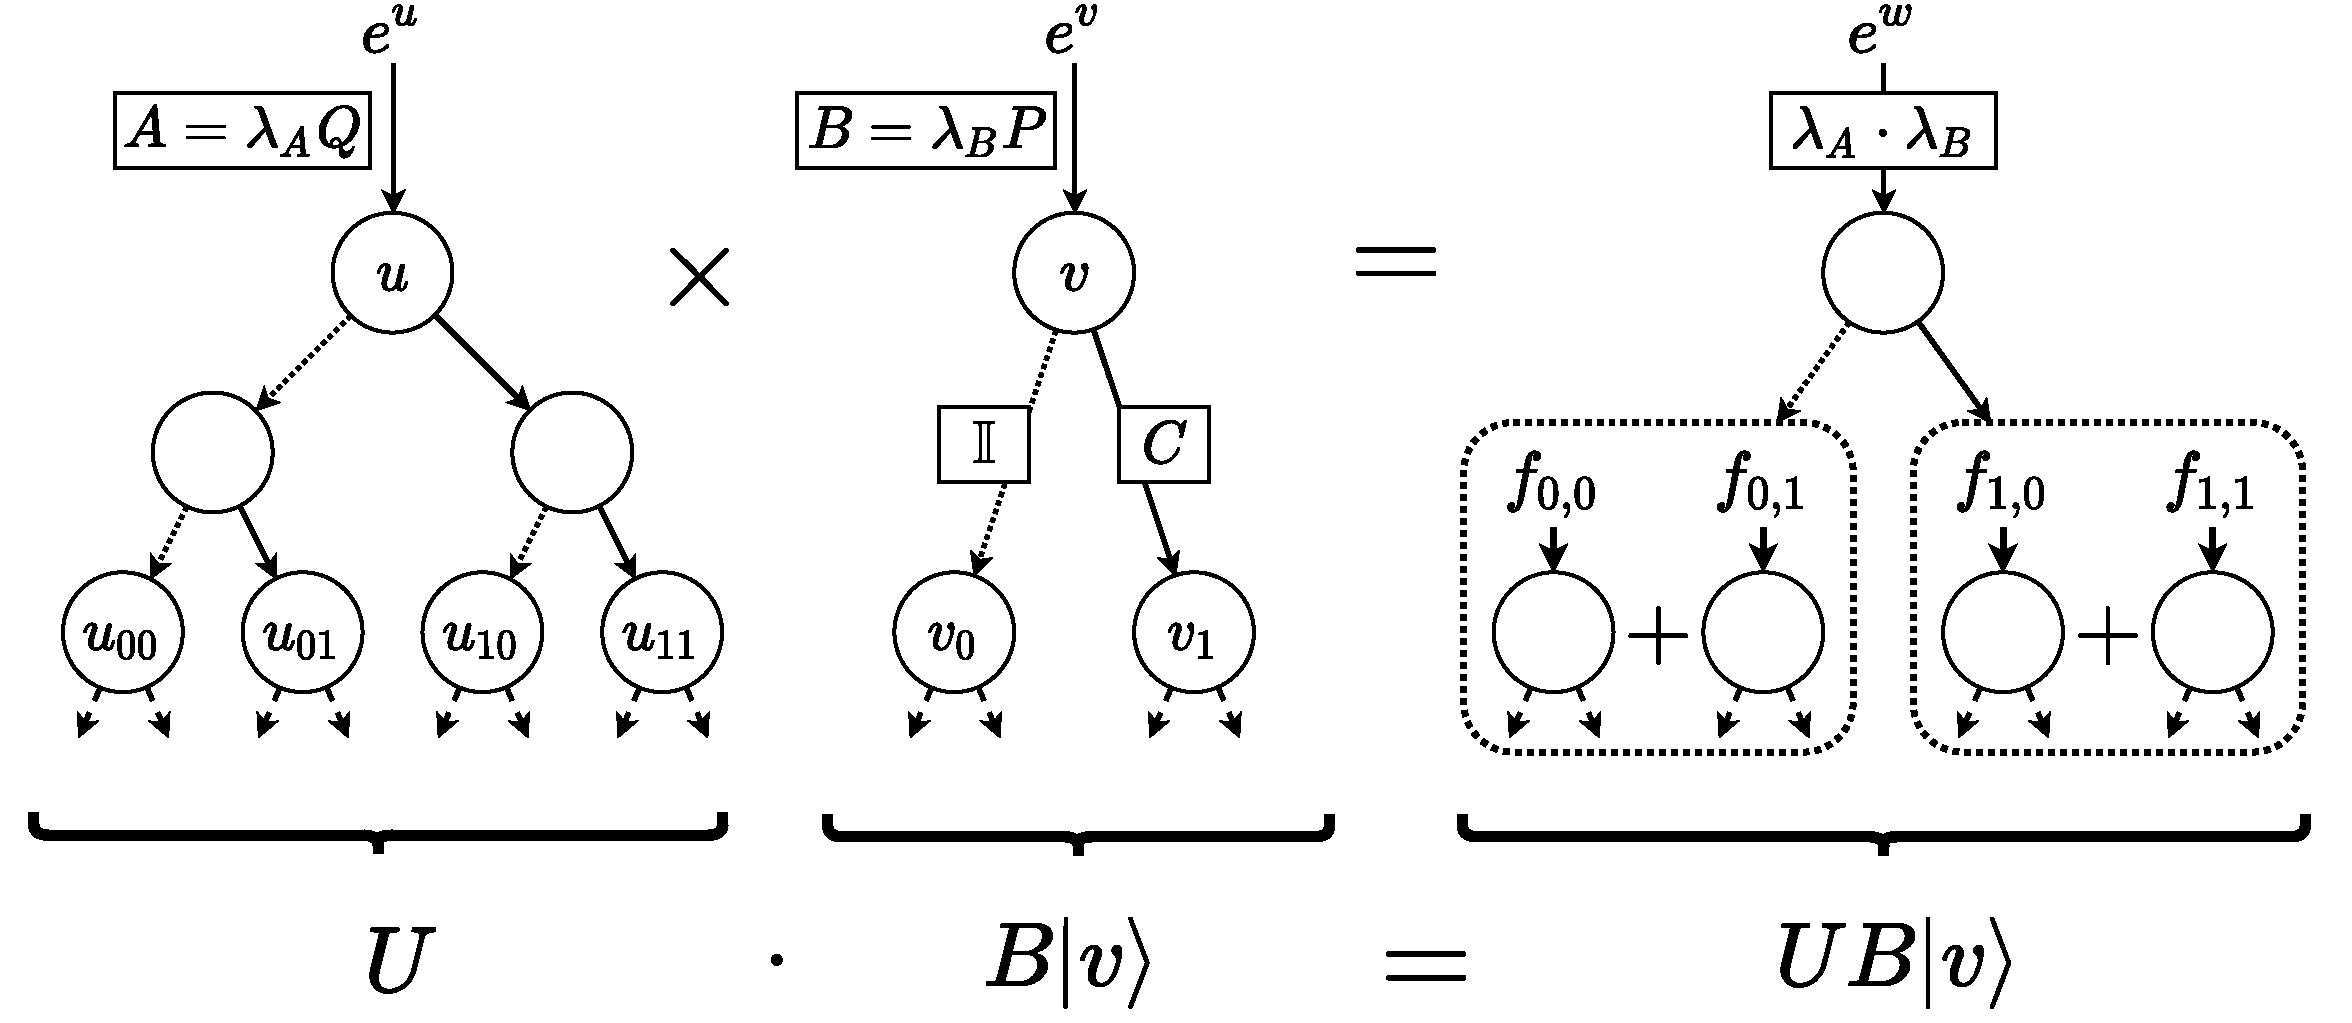
\includegraphics[width=.8\textwidth]{pics/apply-gate-2.pdf}
    \caption{An illustration of \textsc{ApplyGate} (\autoref{alg:apply-gate-limdd-limdd}), where matrix $U$ is applied to state $B\ket{v}$, both represented as Pauli-\limdds.
		The edges $f_{0,0}$, $f_{0,1}$, etc. are the edges made on line \ref{algline:apply-gate-compute-term}.
		The dotted box indicates that these states are added, using \textsc{Add} (\autoref{alg:add-limdds}) before they are passed to \makeedge.
%	For simplicity, this diagram assumes $P_n=\mathbb I$.
%	Notice that the LIM $P^\prime$ is ``propagated'' to the result. In the \textsc{ApplyGate} algorithm, this is accomplished using the $\follow{0}{Av}$ subroutine.
}
	\label{fig:apply-gate}
\end{figure}

The subroutine \textsc{Add} (\autoref{alg:add-limdds}) adds two quantum states, i.e., given two \limdds representing $\ket{e}$ and $\ket{f}$, it returns a \limdd representing $\ket e + \ket f$.
A natural way to implement this algorithm would have been to use the $\follow xe$ procedure to express the states as $\ket{e}=\ket{0}\ket{e_0} + \ket 1\ket{e_1}$ and $\ket{f}=\ket 0\ket{f_0} + \ket 1\ket{f_1}$, and then to call the algorithm recursively to construct the states $\ket{e_0}+\ket{f_0}$ and $\ket{e_1}+\ket{f_1}$.


\begin{algorithm}[b!]
	\begin{algorithmic}[1]
		\Procedure{Add}{\Edge $\ledge[e] Av$, \Edge $\ledge[f] Bw$
		 \textbf{with} $A=\lambda P$, $B=\mu Q$, $\index(v) = \index(w)$}
		\If{$n=0$}
			 \Return $\ledge {A+B}1$ \Comment{$A,B \in \mathbb C$}
		\EndIf
		\If{$v\not\beforeq w$} \Return $\textsc{Add}(f,e)$
		\label{algline:add-swap-for-cache}
		\EndIf
		\State $C:=\rootlabel(\ledge{A^{-1}B}{w})$
		\label{algline:add-factor-out-LIM}
		\If{$(v,\ledge Cw)\in \textsc{Add-cache}$} 
			\Return $A\cdot \textsc{Add-cache}[v,\ledge Cw]$ \Comment{Dynamic programming}
		\EndIf
		\State \Edge $a_0:=\textsc{Add}(\follow 0{\ledge{\mathbb I}v}, \follow 0{\ledge Cw})$
			\label{algline:add-0}
		\State \Edge $a_1:=\textsc{Add}(\follow 1{\ledge{\mathbb I}v}, \follow 1{\ledge Cw})$
			\label{algline:add-1}
		\State \Edge $a:=\makeedge(a_0,a_1)$ 
			\label{algline:add-makeedge}
		\State $\textsc{Add-cache}[v,\ledge Cw]:= a$
            \Comment{Store in dynamic programming cache}
		\State \Return $A\cdot a$
		\EndProcedure
	\end{algorithmic}
	\caption{Given two $n$-LIMDD edges $e,f$, constructs a new LIMDD edge $a$ with $\ket{a}=\ket{e}+\ket{f}$.
	}
	\label{alg:add-limdds}
\end{algorithm}

However, we implement the algorithm slightly differently in order to better take advantage of dynamic programming.
We remark that we are looking to construct the state $A\ket{v} + B\ket{w}$, and that this is equal to $A\cdot (\ket{v}+A^{-1}B\ket{w})$.
Therefore, letting $\ket{\psi}=A^{-1}B\ket{w}$, we use the $\follow x{\ledge{A^{-1}B}w}$ procedure to construct the states $\ket{\psi_0}$ and $\ket{\psi_1}$.
Then, we construct the states $\ket{a_0}=\ket{v_0}+\ket{\psi_0}$ and $\ket{a_1}=\ket{v_1}+\ket{\psi_1}$, on \autoref{algline:add-0} and \ref{algline:add-1}.
Lastly, we construct the state $\ket{a}=\ket{0}\ket{a_0}+\ket 1\ket{a_1}$, on line \ref{algline:add-makeedge}.
Returning the \limdd $A\cdot a$ yields the desired result:
\begin{align}
	A\ket{a} = & A(\ket{0}\ket{a_0}+\ket{1}\ket{a_1}) = A(\ket 0(\ket{v_0}+\ket{\psi_0}) + \ket 1(\ket{v_1}+\ket{\psi_1})) \\
	= & A(\ket{v}+\ket{\psi}) = A(\ket{v} + A^{-1}B\ket{w}) = A\ket{v} + B\ket{w}
\end{align}
We store a tuple $(v,w,C)$ in the cache, where $C=\rootlabel(\ledge {A^{-1}B}w)$ is a canonically chosen LIM such that $C\ket{w}=A^{-1}B\ket{w}$.
By ``canonically chosen'', we mean, again, that the procedure chooses the same $C$ for any input $\ledge Dw, \ledge Ew$ such that $D\ket{w}=E\ket{w}$. 

Finally, on line \ref{algline:add-swap-for-cache}, we use the total order on nodes $\beforeq$,
in order to prevent cache misses due to storing $v$ and $w$ in the wrong order.


%\alfons{It can be implemented in cubic time using the techniques described in } \autoref{sec:preliminaries}.\todo{this should be explained earlier, because it is used in the ApplyGate algorithm.}

%Let us see how implementing the algorithm this way improves the performance of the cache, relative to the straightforward way we have outlined.
%When, after input $(e,f)$, \textsc{Add} is subsequently called as $\textsc{Add}(e'=\ledge {D}{v'},f'=\ledge E{w'})$, then we achieve a cache hit whenever $v=v'$ and $A^{-1}B\ket{w}=D^{-1}E\ket{w'}$, whereas in the simpler implementation, we would have achieved a cache hit only when $A\ket{v}= D\ket{v'}$ and $B\ket{w}= E\ket{w'}$.
%Effectively, this means that we get a cache hit whenever $\ket{e}\simeq \ket{e'}$, instead of when $\ket{e}=\ket{e'}$.

\begin{wrapfigure}{r}{6cm}\vspace{-1em}
    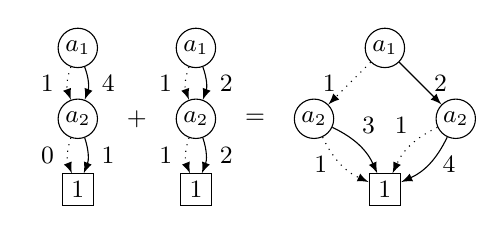
\begin{tikzpicture}[
        scale=0.3,
        every path/.style={>=latex},
        every node/.style={},
        inner sep=0pt,
        minimum size=0.5cm,
        line width=1pt,
        thin,
        font=\small
        ]

        % nodes

        % nodes
        \node[draw,circle] (a1) at ( 0,-0)     {$a_1$};
        \node[draw,circle] (a2) at (0,-3) {$a_2$};

        \node[draw,circle,rectangle,minimum size=0.4cm] (w1) at ( -0,-6) {$1$};

        % edges
        \draw[dotted,bend left=-20] (a1) edge  node[left] {$1$} (a2);
        \draw[bend left=20]        (a1) edge  node[right] {$4$} (a2);
        
        \draw[dotted,bend left=-20] (a2) edge node[left] {$0$} (w1);
        \draw[bend left=20]       (a2) edge  node[right] {$1$} (w1);


        \node[draw,circle] (a1) at (5,-0)     {$a_1$};
        \node[draw,circle] (a2) at (5,-3) {$a_2$};

        \node[draw,circle,rectangle,minimum size=0.4cm] (w1) at ( 5,-6) {$1$};

        % edges
        \draw[dotted,bend left=-20] (a1) edge  node[left] {$1$} (a2);
        \draw[bend left=20]        (a1) edge  node[right] {$2$} (a2);
        
        \draw[dotted,bend left=-20] (a2) edge node[left] {$1$} (w1);
        \draw[bend left=20]       (a2) edge  node[right] {$2$} (w1);


        \node[draw,circle] (a1p) at ( 13,-0)     {$a_1$};
        \node[draw,circle] (a20) at ( 10,-3) {$a_2$};
        \node[draw,circle] (a21) at ( 16,-3) {$a_2$};

        \node[draw,circle,rectangle,minimum size=0.4cm] (w1) at ( 13,-6) {$1$};

        % edges
        \draw[dotted] (a1p) edge  node[left] {1} (a20);
        \draw[]     (a1p) edge  node[right] {2} (a21);
        
        \draw[dotted,bend left =-20] (a20) edge  node[left] {1} (w1);
        \draw[      ,bend left = 20]       (a20) edge  node[above right, xshift=-4pt] {3} (w1);
        
        \draw[dotted,bend left =-20] (a21) edge node[above left, xshift=4pt] {1} (w1);
        \draw[      ,bend left = 20]       (a21) edge  node[right] {4} (w1);
        
        
        \node[] (a2) at (2.5,-3) {$+$};
        \node[] (a2) at (7.5,-3) {$=$};
        
    \end{tikzpicture}
    \caption{Adding two states \vect{0,1,0,4} and \vect{1,2,2,4} as \qmdds can cause an exponentially larger result \qmdd  \vect{1,3,2,8} due to the loss of common factors.}
    \label{fig:explosion}
\end{wrapfigure}

The worst-case running time of \textsc{Add} is $\oh(n^32^n)$, if $n$ is the number of qubits.
The resulting \limdd can be exponential in the input sizes (bounded by $2^n$),
and \textsc{Add} calls \makeedge has runtime $\oh(n^3)$.
This exponential result happens already for \qmdds because the addition might remove any common factors that can be factored out as illustrated in \autoref{fig:explosion}.
%every recursive call effects a cache miss, so that in total $\oh(2^n)$ recursive calls are made.
This exponential-time worst-case behavior  for \qmdds (and related DDs)
 was identified \cite[Table 2]{fargier2014knowledge} and is inherited by \limdds.
However, the \textsc{Add} algorithm is polynomial-time when $v=w$ and $v$ is a stabilizer state (\autoref{thm:only-linear-recursive-add-calls-general})
% Note however, that the corresponding \add would already be exponential


\subsection{The \makeedge subroutine}
\label{sec:makeedge}


To construct new nodes and edges, our algorithms use the \makeedge subroutine as discussed above.
\makeedge produces reduced parent nodes for reduced children, so that the \limdd representation becomes canonical; an important property for efficient manipulation algorithms and analysis techniques. 
Here we give the algorithm for \makeedge and show that it runs in time $O(n^3)$ (assuming the input nodes are reduced).

%\todo[inline]{I think \autoref{sec:makeedge-basic-reduction} makes nodes reduced, not semi-reduced? Let me double-check -LV}
We call a \limdd node \concept{semi-reduced}, if it satisfies the
{low factoring, low precedence, zero edge and merge rules} of \autoref{def:reduced-limdd}, i.e., if it satisfies all reduction rules except possibly high determinism.
Semi-reduction is easy to enforce, as shown in \autoref{sec:makeedge-basic-reduction}.
The bulk of this section discusses how to obtain a canonical LIM on the high edge
to realize high determinism.
We achieve this  in \autoref{sec:choose-canonical-isomorphism-pauli} by selecting a lexicographically minimum LIM from all the candidates.
The problem of find all candidates efficiently is reduced to finding all stabilizers of a state $\ket v$,
i.e., the set of all LIMs $A$ such that $A \ket v = \ket v$, efficiently represented as a set of generators (see also \autoref{sec:preliminaries}).
In \autoref{sec:pauli-isomorphism-detection}, we show how to compute these stabilizers in the bottom-up fashion typical for decision diagrams.


%\begin{lemma}
%    For any Tower \limdd, the procedure  \textsc{Add} takes $\oh(n^4)$ time.   
%\end{lemma}
%\begin{proof}
%    Let $\ledge {B_n}{v_n}$ be the root edge of a Tower  with nodes $v_n, \dots v_1, v_0 = \leaf$ and edges
%    $\Low = \High = \set{ (v_i, v_{i-1}) \mid i \in \set{0, \dots, n} }$ with labels
%    $\lbl(\high{v_i}) = B_i$, $\lbl(\low{v_i}) = \id$.   
%    Using induction, we find that in the base case $n=0$, $B_n$ is a scalar so the resulting 
%\end{proof}


\subsubsection{Basic reduction in MakeEdge}
\label{sec:makeedge-basic-reduction}

%\todo[inline]{Question 2: Why is it called a root edge, when most nodes are not the root? If I look in \autoref{def:limdd}, then the root node is the distinguished top node. Maybe we should call it, ``incoming edge''? -LV One way to view it is that our algorithms create many \limdds (some overlapping). Because it is all sequential, usually only one or two exist at the same time.}

\autoref{alg:make-edge} gives the \makeedge subroutine that now
constructs canonical nodes through reduction, yielding a new root edge (whose LIM label is not necessarily canonical).
It takes as input two edges $e_0$ and $e_1$, pointing to already reduced nodes, and outputs an edge $e$, pointing to a reduced node $v$,
such that $\ket{e}=\ket{0}\ket{e_0}+\ket{1}\ket{e_1}$.
The reduction proceeds as follows.
\begin{itemize}
    \item 
First it ensures low precedence, switching $e_0$ and $e_1$ if necessary at
\autoref{l:swap}. This is also done if $e_0$'s label $A$ is $0$ to allow for low factoring (avoiding divide by zero).
    \item 
Low factoring, i.e., dividing
out the LIM $A$, placing it on the root node,
        is visualized in \autoref{fig:reduced1} for the cases $e_1 = 0 / e_1\neq 0$,
and done in the algorithm at \autoref{l:low1},\ref{l:low2} / \ref{l:low3},\ref{l:low4}.
\item 
The zero edges rule is enforced in the $B=0$ branch by taking $v_1 := v_0$.
\item 
The canonical high label $\highlim$ is computed by \textsc{GetLabels},
    discussed below, for low factored node $\lnode[w] {\id}{v_0}{\hat A}{v_1}$.
    It satisfies the high determinism rule of \autoref{def:reduced-limdd} with $\highlabel(w)= \highlim$
    as shown in the next section with \autoref{cor:highlabel}.
\item
Finally, we merge nodes by creating an entry $(v_0,\highlim,v_1)$ in 
a \concept{unique table}~\cite{brace1990efficient} at \autoref{algline:find-v-in-unique}. 
\end{itemize}

All steps except for \textsc{GetLabels} have complexity $O(1)$ or $O(n)$ (for checking low precedence, we use nodes' order in the unique table).
\textsc{GetLabels} has a runtime $O(n^3)$ as we show in \autoref{sec:choose-canonical-isomorphism-pauli}, yielding an overall complexity $O(n^3)$.
%\todo{I think the reducedness of the children is no longer required, provided we phrase the resulting reduction as dependent on the reducedness of these inputs.}

\begin{algorithm}
	\begin{algorithmic}[1]
        \Procedure{MakeEdge}{\Edge $\ledge[e_0]{A}{v_0}$, \Edge $\ledge[e_1]{B}{v_1}$ 
                        , where $v_0, v_1$ reduced, \textbf{with} $A \neq 0$ \textbf{or} $B \neq 0$}
%    		\State \textbf{assert} $\index(v_0) = \index(v_1)$
%    		\State $n := \index(v_0)$
            \If{$v_0\not\beforeq v_1$ \textbf{or} $A=0$} \Comment{Enforce \textbf{low precedence} and enable \textbf{factoring}}
                \State \Return\label{l:swap}
                        $(X \otimes \unit_2^{\otimes n})\cdot \text{MakeEdge}(e_1, e_0)$
                        %\ledge{B}{v_1},\ledge{A}{v_0})$
%                \todo[inline]{Tim: do we already have notation for multiplying an edge with a LIM?} %Alfons: Yes. See table
			\EndIf
            %
            %
%            \Comment{Enforce \textbf{low factoring}}
%            \State $w_0 := v_0$
            \If{$B = 0$}
            \State $v_1 := v_0$     \Comment{Enforce  \textbf{zero edges}}
            \State $v := \lnode{\unit_2^{\otimes n}}{v_0}{0}{v_0}$\label{l:low1}
            \Comment{Enforce \textbf{low factoring}}
%            \State $\highlim := 0$
%            \State $w_1 := v_0$
%			\Comment{Enforce \textbf{}}
            %
            %
            \State $\rootlim := \unit_2 \otimes A$   \Comment{$\rootlim \ket v = \ket 0 \otimes 
                                        A \ket{v_0} + \ket 1 \otimes  B \ket{v_1}$}\label{l:low2}
            \Else
            %
            %
            \State $\hat A := A^{-1}B$ \Comment{Enforce \textbf{low factoring}}\label{l:low3}
            \State $\highlim, \rootlim:=\textsc{GetLabels}(\hat A,v_0,v_1)$
            \label{algline:makeedge-get-labels}
            \Comment{Enforce \textbf{high determinism}}
            \State $v := \lnode{\unit_2^{\otimes n}}{v_0}{\highlim}{v_1}$ 
             \Comment{$\rootlim \ket v = \ket 0 \otimes 
                                         \ket{v_0} + \ket 1 \otimes A^{-1} B \ket{v_1}$}
                \label{l:low4}
            \State $\rootlim := (\id[2] \otimes A) \rootlim $ 
             \Comment{$(\id[2] \otimes A)\rootlim \ket v = \ket 0 \otimes  A \ket{v_0} + \ket 1 \otimes  B \ket{v_1}$}
            \EndIf
%			\State node $v := Node(v_0,v_1,\hat A)$ representing $\ket{0}\ket{v_0}+\ket{1}\hat A\ket{v_1}$
			\State $v^r:=$ Find or create unique table entry $\unique[v] = (v_0, \highlim, v_1)$       
			\label{algline:find-v-in-unique}
            \Comment{Enforce \textbf{merge}}
            \State \Return $\ledge{\rootlim}{v^r}$
		\EndProcedure
	\end{algorithmic}
	\caption{
        Algorithm \makeedge takes two root edges to (already reduced) nodes $v_0,v_1$, the children of a new node, and returns a reduced node with root edge.
	It assumes that %the children have the same qubit-index, i.e., 
	$\index(v_0) = \index(v_1) = n$.
%	For sake of simplicity, this algorithm does not enforce the root edge determinism rule, nor the zero edges rule.
	We indicate which lines of code are responsible for which reduction rule in \autoref{def:reduced-limdd}.
}
	\label{alg:make-edge}
\end{algorithm}

\begin{figure}
    % CASE: different children nodes
\tikz[->,>=stealth',shorten >=1pt,auto,node distance=1.5cm,
        thick, state/.style={circle,draw,inner sep=0pt,minimum size=18pt}]{
    %\node[state, above = 2cm of 1, xshift=3.3cm] (top) {};

    \node[state] (2) {$w$};
    \node[state] (1a) [below = 1cm of 2, xshift=1.3cm] {$v_0$};
    \node[right = 0.25cm of 1a] () {$\beforeq$};
    \node[state] (1b) [below = 1cm of 2, xshift=2.8cm] {$v_1$};
    \node[above = 0.5cm of 2,xshift=1.95cm,fill=black] (x)  {};
    \path[]
    (x) edge[bend left=-20]    node[above right,pos=.8] {} (2)
    (2) edge[e0] node[pos=.5,left] {$\id[2]^{\otimes n}$} (1a)
    (2) edge[e1] node[pos=.15,right, xshift = .5cm] {$\lambda P$} (1b)
    ;
    
    \node[state, right = 3.3cm of 2] (4) {$v^{\textnormal{r}}$};
%    \node[above = 0.5cm of 4] (x)  {};
    \path[]
    (x) edge[bend left=20]     node[pos=.9] {
        $\rootlim = \left(\lambda X\otimes P\right)^{x} \cdot
        \left(Z^s \otimes \left(\gmax_0\right)^{-1}\right)$
        } (4)
    (4) edge[e0] node[pos=.3,above left] {$\id[2]^{\otimes n}$} (1a)
    (4) edge[e1] node[pos=.3,below right] {
%    \begin{minipage}{5cm}
        $\highlim = %(-1)^s \cdot \lambda^{(-1)^x} \cdot \gmax_0 \cdot P \cdot \gmax_1 = 
%                    \displaystyle \min_{i,s,x \in \{0, 1\},g_i \in \Aut(v_i)}(\textnormal{\sc EligibleHigh}_{x,s,g_0,g_1})
%			\displaystyle \min_{i,x\in \{0,1\},g_{0/1}\in \Stab(v_{0/1})}
			(-1)^s\lambda^{(-1)^x}g_0Pg_1
        $
%    \end{minipage}
    } (1b)
    (2) --  node[yshift=.1cm] {$\rightsquigarrow$} (4)
    (1a)  edge[loop left, dashed] node[left]{$g_0\in\Aut(v_0)$} (1a)
    (1b)  edge[loop right, dashed] node[right]{$\Aut(v_1) \ni g_1$} (1b)
    ;
    }
    %
    %
    %
    \vspace{1mm}
    \newline
    \centering
    Choose $s,x\in \{0,1\},g_0\in \Stab(v_0),g_1\in \Stab(v_1)$ s.t. $\highlim$ is minimal and $x=0$ if $v_0=v_1$.
    %$
%    \highlim=\displaystyle \min_{i,x\in \{0,1\},g_{0/1}\in \Stab(v_{0/1})}(-1)^s\lambda^{(-1)^x}g_0Pg_1
%    \textnormal{\sc EligibleHigh}_{x,s,g_0,g_1}  \defn
%        \set{(-1)^s \cdot \lambda^{(-1)^x} \cdot g_0 \cdot P \cdot g_1 ~\Big|~ %g_i \in \Aut(v_i),
        %\quad , \quad 
%         x \neq 1 \text{ if } v_0 \neq v_1 }
%     $
    %
	\caption{
        Illustration of finding a canonical high label for a semi-reduced node $w$,
        yielding a reduced node $v^{\text{r}}$.
%         which satisfies Low Precedence ($v_0 \beforeq v_1$) and Low Factoring (low edge is $\id[2]^{\otimes n}$).
The chosen high label is the minimal element from the set of eligible high labels
based on stabilizers $g_0,g_1$ of $v_0,v_1$ (drawn as self loops).
The minimal element holds a factor $\lambda^{(-1)^x}$ for some $x \in \{0, 1\}$.
There are two cases: if $v_0 \neq v_1$ or $x=0$, then the factor is $\lambda$ and the root edge should be adjusted with an $\id[2]$ or $Z$ on the root qubit.
The other case, $x=1$, leads to an additional multiplication with an $X$ on the root qubit.
%The result is a node $v^{\textnormal{reduced}}$ which satisfies Low Precedence, Low Factoring and High Determinism.
}
	\label{fig:reduced}
\end{figure}


%\todo[inline]{first explain the data structure \automorphismgenerators, i.e. that it can be thought of as spanning a vector space, and then give the algorithm}


%Data structure {\sc SystemOfPauliEquations}
%is a list of equations of the form $\lambda P (\alpha \ket{\phi}) = \beta \ket{\psi}$.
%Has a method {\sc 


\subsubsection{Choosing a canonical high-edge label}
\label{sec:choose-canonical-isomorphism-pauli}

%The \textsc{MakeEdge} procedure enforces that all reduction rules are satisfied, one by one.
%For all reduction rules except for a canonical high-label choice this is straightforward, e.g. for Low Precedence, if the right child $\succ$ the left child, then swap them and apply the appropriate Pauli at the root label.

On line \ref{algline:makeedge-get-labels}, the \makeedge algorithm finds a canonical label $\highlim$ for the high edge of node $v$ with a call to \textsc{GetLabels}.
%The semi-reduced node  \lnode[w]{\unit_2^{\otimes n}}{v_0}{\hat A}{v_1} with $v_0 \neq v_1$ created in
%\makeedge is passed to \textsc{GetLabels} to obtain a canonical
%representative \lnode[v^{\text{r}}]{\unit_2^{\otimes n}}{v_0}{\highlim}{v_1}
% (with `r' for reduced) and a root edge $\ledge[e] {\rootlim}{v^{\text{r}}}$ such that
% $\ket e = \ket w$.
It does so by taking the lexicographically minimal candidate for \highlim, see \autoref{sec:preliminaries}.
We now first characterize all eligible labels \highlim, by reducing the problem to finding stabilizer subgroups of the children nodes $v_0,v_1$ (see \autoref{sec:preliminaries}), denoted as $\Stab(v_0)$ and $\Stab(v_1)$.
Then, we show that \textsc{GetLabels} (\autoref{alg:find-canonical-edges}) correctly finds the lexicographically minimal eligible LIM (and corresponding root label), and runs in time $O(n^3)$ where $n$ is the number of qubits.

\autoref{fig:reduced} illustrates this process.
It shows the status of the \makeedge algorithm on line \ref{algline:makeedge-get-labels}, when it has enough information to construct the semi-reduced node $\lnode[w]{\id^{\otimes n}}{v_0}{\hat A}{v_1}$, with $\hat A=\lambda P$ on its high edge, shown on the left.
The set of eligible high labels is shown, and the lexicographically minimal is chosen as $\highlim$, yielding a new node $v^r$ (with `r' for `reduced').
This set of labels is decomposed into a choice of $v_0,v_1$ stabilizer $g_0, g_1$ and a choice for the most significant
\Pauli operator on the root LIM $X^x Z^s$.
\autoref{thm:eligible-isomorphisms-pauli} shows that this captures all possible high edges.



%\begin{lemma}
%    \label{lemma:isomorphic-nodes-have-same-high-label-scalar}
%    Let $\lambda, \mu \in \mathbb{C}$ and let $A, B$ be Pauli strings of length $n$.
%    Furthermore, let $v$ be the $n$-qubit root node of a reduced Pauli-\limdd.
%    If $\ket{\lambda A} \psim \ket{\mu B}$, then $\lambda = \mu$.
%\end{lemma}
%\begin{proof}
%    By induction...still to do
%\end{proof}



%\todo[inline]{Tim: maybe we should instead of Automorphism group, talk about Stabilizer group. Potential disadvantage is that readers who skim the work incorrectly assume that this is about groups which characterize stabilizer states, i.e. the group is maximal, making our algorithms look like a new (and stupid) way to simulate stabilizer states}

\begin{theorem}
    [Eligible high-edge labels]
	\label{thm:eligible-isomorphisms-pauli}
    Let $\lnode[w]{\id[2]^{\otimes n}}{v_0}{\lambda P}{v_1}$ be a semi-reduced $n$-qubit node
    in a Pauli-\limdd, where $v_0, v_1$ are reduced, $P$ is a Pauli string and $\lambda \neq 0$.
    For all nodes $v = \lnode[v]{\id[2]^{\otimes n}}{v_0}{\highlim}{v_1}$, it holds that $\ket{w} \simeq \ket{v}$  if and only if 
    %\todo[inline]{Tim: I just realised that the statement should be: for all semi-reduced $w$: $\ket{w} \simeq \ket{v}$ if and only if $w$ has children $v_0$ and $v_1$, and the eligible high labels are of the form \dots. Should redo}
    \begin{equation}
        \label{eq:eligible-high-label}
    \highlim = (-1)^s \cdot \lambda^{(-1)^x} g_0 P g_1
    \end{equation}
        for some $g_0 \in \Aut(v_0), g_1 \in \Aut(v_1), s,x\in \{0, 1\}$ and
        $x=0$ if $v_0 \neq v_1$.
    An isomorphism mapping $\ket{w}$ to $\ket{v}$ is 
    \begin{equation}
        \label{eq:root-label-eligible-high-label}
        \rootlim = (X \otimes \lambda P)^{x} \cdot (Z^s \otimes (g_0)^{-1}).
    \end{equation}
\end{theorem}
\begin{proof}
    It is straightforward to verify that the isomorphism $\rootlim$ in eq.~\eqref{eq:root-label-eligible-high-label} indeed maps $\ket{w}$ to $\ket{v}$ (as $x = 1$ implies $v_0 = v_1$), which shows that $\ket{w} \simeq \ket{v}$.
    For the converse direction, suppose there exists an $n$-qubit Pauli LIM $C$ such that $C\ket{w} = \ket{v}$, i.e.
    \begin{equation}
        \label{eq:eligible-proof}
        C
        \left(\ket{0}\otimes \ket{v_0} + \lambda \ket{1} \otimes P \ket{v_1}\right)
        =
        \ket{0}\otimes \ket{v_0} + \ket{1} \otimes \highlim \ket{v_1}
        .
    \end{equation}
    We show that if $\highlim$ satisfies eq.~\eqref{eq:eligible-proof}, then it has a decomposition as in eq.~\eqref{eq:eligible-high-label}.
    \def\brest{C_{\textnormal{rest}}}
    \def\qtop{Q_{\textnormal{top}}}
    We write $C = \qtop \otimes \brest$ where $\qtop$ is a single-qubit Pauli operator and $\brest$ is an $(n-1)$-qubit Pauli LIM (or a complex number $\neq 0$ if $n=1$).
    We treat the two cases $\qtop \in \{\unit_2, Z\}$ and $\qtop \in \{X, Y\}$ separately:

    \textbf{Case $\boldsymbol{\unit_2, Z}$.} Then $\qtop = \begin{smallmat} 1& 0\\0 & (-1)^y\end{smallmat}$ for $y \in \{0, 1\}$.
        In this case, eq.~\eqref{eq:eligible-proof} implies $\brest \in \Aut(\ket{v_0})$ and $(-1)^y\lambda \brest P \ket{v_1} = \highlim \ket{v_1}$, or, equivalently, $(-1)^{-y} \lambda^{-1} P^{-1} \brest^{-1} \highlim \in \Aut(v_1)$.
        Hence, by choosing $s = y$ and $x = 0$, we compute
        \[
            (-1)^y \lambda^{(-1)^0} \underbrace{\brest}_{\in \Aut(v_0)} P \underbrace{(-1)^{-y} \lambda^{-1} P^{-1} \brest^{-1} \highlim}_{\in \Aut(v_1)}
            =
            \frac{(-1)^{y} \lambda^{(-1)^0}}{ (-1)^y \lambda} \highlim
            =
            \highlim
        \]
    \textbf{Case $\boldsymbol{X, Y}$.} Write $\qtop = \begin{pmatrix}0& z^{-1}\\ z&0\end{pmatrix}$ where $z \in \{1, i\}$. Now, eq.~\eqref{eq:eligible-proof} implies
		\begin{equation}
		    \label{eq:z}
            z \brest \ket{v_0} = \highlim \ket{v_1}
		\qquad\textnormal{and}\qquad
            z^{-1} \lambda \brest P \ket{v_1} = \ket{v_0}.
		\end{equation}
From eq.~\eqref{eq:z}, we first note that $\ket{v_0}$ and $\ket{v_1}$ are isomorphic, so by Corollary~\ref{cor:node-canonicity-strong}, we have $v_0 = v_1$.
    Consequently, we find from eq.~\eqref{eq:z} that $z^{-1}\brest^{-1} \highlim \in \Aut(v_0)$ and $z^{-1}\lambda \brest P \in \Aut(v_1)$.
    Now choose $x=1$ and choose $s$ such that $(-1)^s \cdot z^{-2} \brest^{-1} \highlim \brest = \highlim$ (recall that Pauli LIMs either commute or anticommute, so $\highlim\brest = \pm \brest \highlim$).
    This yields:
    \[
        (-1)^s \lambda^{-1} \cdot \underbrace{z^{-1}\brest^{-1} \highlim}_{\in \Aut(v_0)} \cdot P \cdot \underbrace{z^{-1} \lambda P \brest}_{\in \Aut(v_1)}
        =
        \lambda^{-1} \cdot \lambda \cdot
        (-1)^s 
        z^{-2} \cdot \left(\brest^{-1} \highlim \brest \right)
        =
        \highlim
    \]
    where we used the fact that $P^2 = \id[2]^{\otimes (n-1)}$ because $P$ is a Pauli string.
\end{proof}

%Next, we define a lexicographic ordering on LIMs:

\begin{corollary}\label{cor:highlabel}
As a corollary of \autoref{thm:eligible-isomorphisms-pauli}, we find that taking, as in \autoref{fig:reduced},
\[
\highlabel(\lnode[v] {\id}{v_0}{\lambda P}{v_1}) = \displaystyle \min_{\hspace{-3mm} i,s,x \in \{0, 1\},g_i \in \Aut(v_i)}(\set{(-1)^s \cdot \lambda^{(-1)^x} \cdot g_0 \cdot P \cdot g_1 ~\Big|~ 
         x \neq 1 \text{ if } v_0 \neq v_1 })
\]
yields a proper implementation of \highlabel as required by \autoref{def:reduced-limdd},
because it considers all possible \highlim such that
$\ket v \simeq_{\Pauli} \ket{0}\ket{v_0}+\ket{1}\otimes \highlabel(v)\ket{v_1}$.
\end{corollary}



% todo the procedure which chooses the lexmin element, not which constructs the isomorphism; this causes confusion

%, with high edge label $\lambda P$ and children $v_0, v_1$ as input, computes the minimal eligible high edge label and the root edge label that preserves the represented quantum state.
A naive implementation for \textsc{GetLabels} would follow the possible decompositions of eligible LIMs (see eq.~\eqref{eq:eligible-high-label}) and attempt to make this LIM smaller by greedy multiplication, first  with stabilizers of
$g_0 \in \Aut(v_0)$, and then with stabilizers $g_1\in \Aut(v_1)$.
To see why this does not work, consider the following example:
the high edge label is $Z$ and the stabilizer subgroups $\Aut(v_0) = \langle X\rangle$ and $\Aut(v_1) = \langle Y \rangle$.
Then the naive algorithm would terminate and return $Z$ because $X, Y> Z$, which is incorrect since the high-edge label $X \cdot Z \cdot Y = -i \id[2]$ is smaller than $Z$.

\begin{algorithm}
	\caption{
		Algorithm for finding the LIMs $\highlim$ and $\rootlim$ required by \makeedge.
		The LIM $\highlim$ is chosen canonically as the lexicographically smallest LIM in 
		the set characterized in \autoref{thm:eligible-isomorphisms-pauli}.
		It runs in $O(n^3)$-time (with $n$ the number of qubits),
		provided $\getautomorphisms$ has been computed for the children $v_0, v_1$.
		\label{alg:find-canonical-edges}
	}
	\begin{algorithmic}[1]
		\Procedure{GetLabels}{PauliLim $\lambda P \neq 0$ (current high label), reduced children nodes $v_0, v_1$}
		\Statex \textbf{Output}: canonical high label $\highlim$ and root label $\rootlim$
		\State $G_0, G_1 := \getautomorphisms(v_0), \getautomorphisms(v_1)$
		\State $(g_0, g_1) := \textsc{ArgLexMin}(G_0, G_1, \lambda P)$
%		\label{line:getlabels-min}
		\label{line:getlabels-argmin}
%		\State $A := \lambda P \cdot g_0 \cdot g_1$
%		\Comment $A = \textsc{LexMin}(G_0, G_1, \lambda P)$
		%        \State \textbf{if} $P$ and $g_0$ commute \textbf{then} $t:=0$ \textbf{else} $t:=1$
		%        \label{line:sign-error}
		%        \Comment $A =  (-1)^t \cdot g_0 \cdot \lambda P \cdot g_1$
		%
		\If{$v_0=v_1$}
		\label{algline:getlabels-start-minimizing}
		\State $(x,s):=\displaystyle\argmin_{(x,s)\in\{0,1\}^2}(-1)^s\lambda^{(-1)^x}g_0Pg_1$
		\Else
		\State $x:=0$
		\State $s:=\displaystyle \argmin_{s\in \{0,1\}} (-1)^s\lambda g_0Pg_1$
		\label{line:minimized-lim} 
		\EndIf
		%        \State $x := 0$
		%        \If {$v_0 = v_1$}  x  := $\displaystyle\argmin_{ 
		%             x\in \set{0, 1}}  
		%        \set{ (-1)^t \cdot \lambda^{(-1)^x} \cdot g_0 \cdot P \cdot g_1}$
		%        \Comment see \autoref{thm:eligible-isomorphisms-pauli}
		%        \EndIf
		%        \State $s:= \displaystyle\argmin_{s\in \set{0,1}}\set{(-1)^s\cdot (-1)^t \lambda^{(-1)^x} \cdot g_0 \cdot  P  \cdot g_1} $
		\State $\highlim := (-1)^s \cdot \lambda^{(-1)^x} \cdot g_0 \cdot P \cdot g_1$
		\State $\rootlim := (X \otimes \lambda P)^{x} \cdot (Z^s \otimes (g_0)^{-1})$
		%
		\State \Return $(\highlim, \rootlim)$
		\EndProcedure
	\end{algorithmic}
\end{algorithm}

To overcome this, we consider the group closure of \emph{both} $\Aut(v_0)$ \emph{and} $\Aut(v_1)$.
See \autoref{alg:find-canonical-edges} for the $O(n^3)$-algorithm for \textsc{GetLabels}, which proceeds in two steps.
In the first step (\autoref{line:getlabels-argmin}), we use the subroutine \textsc{ArgLexMin} for finding the minimal Pauli LIM $A$ such that $A = \lambda P \cdot g_0 \cdot g_1$ for $g_0\in \Aut(v_0), g_1\in \Aut(v_1)$.
We will explain and prove correctness of this subroutine below in \autoref{sec:lexmin}.
%Next, note that the eligible-high-label expression in eq.~\eqref{eq:eligible-high-label} contains the factor $g_0 \cdot \lambda P \cdot g_1$ instead of $\lambda P \cdot g_0 \cdot g_1$; however, these differ by a factor $\pm 1$ because Pauli LIMs either commute or anticommute.
%This potential sign error is corrected in \autoref{line:sign-error}.
In the second step (Lines \ref{algline:getlabels-start-minimizing}-\ref{line:minimized-lim}), we follow eq.~\eqref{eq:root-label-eligible-high-label} by also minimizing over $x$ and $s$.
Finally, the algorithm returns $\highlim$, the minimum of all eligible edge labels according to eq.~\eqref{eq:root-label-eligible-high-label}, together with a root edge label $\rootlim$ which ensures the represented quantum state remains the same.

Below, we will explain $O(n^3)$-time algorithms for finding generating sets for the stabilizer subgroup of a reduced node and for \textsc{ArgLexMin}.
Since all other lines in \autoref{alg:find-canonical-edges} can be performed in linear time, its overall runtime is $O(n^3)$.
Note that we can amortize $\getautomorphisms$ over the \makeedge calls.









%We now define the \highlabel~function, which computes the canonical root label following \autoref{def:reduced-limdd}, as the function invoking \autoref{alg:find-canonical-edges} on a semi-reduced node $\lnode{\id}{v_0}{\lambda P}{v_1}$ and returning $\highlabel$.
%Above, we have argued that $\highlabel$ thus returns the minimal eligible high label.
%It follows immediately from this fact that \highlabel~is correct, i.e. it obeys its requirement in \autoref{def:reduced-limdd}.

%\begin{lemma}
%    Let $v_0, v_1$ be reduced $n$-qubit nodes, and $A$ an $n$-qubit Pauli LIM.
%    Then \autoref{alg:find-canonical-edges} on input $(A, v_0, v_1)$, outputs 
%            $\displaystyle \min_{\textnormal{$n$-Pauli LIM} B} \{B \mid  B\ket{v_A} = \ket{v_B}\}$,\todo{$B \in $ ?}
%    where we have denoted $\ket{v_C} = \ket{0}\otimes\ket{v_0} + \ket{1} \otimes C \ket{v_1}$ for a Pauli LIM $C$
%    and a \alfons{semi-reduced node $v_C$}.
%\end{lemma}
%\begin{proof}
%    \todo[inline]{TODO}
%\end{proof}






\subsubsection{Constructing the stabilizer subgroup of a \limdd node}
\label{sec:pauli-isomorphism-detection}

In this section, we give a recursive subroutine \getautomorphisms to construct the stabilizer subgroup $\Aut(\ket{v}) := \{A \in \paulilim_n \mid A\ket{v} = \ket{v}\}$ of an $n$-qubit \limdd node~$v$ (see \autoref{sec:preliminaries}).
The subroutine is used by the algorithm \textsc{GetLabels} to select a canonical label for the high edge and root edge.
If the stabilizer subgroup of $v$'s children have been computed already, \getautomorphisms's runtime is $O(n^3)$.
\getautomorphisms returns a generating set for the group $\Stab(\ket{v})$.
Since these stabilizer subgroups are generally exponentially large in the number of qubits $n$, but they have at most $n$ generators, storing only the generators instead of all elements may save an exponential amount of space.
%Each $n$-qubit stabilizer subgroup has a generator set of size at most $n$.
Because any generator set $G$ of size $|G|>n$ can be brought back to at most $n$ generators in time $\oh(|G| \cdot n^2)$ (see \autoref{sec:preliminaries}), we will in the derivation below show how to obtain generator sets of size linear in $n$ and leave the size reduction implicit.
We will also use the notation $A \cdot G$ and $G \cdot A$ to denote the sets $\{A \cdot g | g\in G\}$ and $\{g \cdot A | g \in G\}$, respectively.

We now sketch the derivation of the algorithm.
The base case of the algorithm is the Leaf node of the \limdd, representing the number $1$, which has stabilizer group $\{1\}$.
For the recursive case, we wish to compute the stabilizer group of a reduced $n$-qubit node $v=\lnode[v]{v_0}{\mathbb I}{\highlim}{v_1}$.
If $\highlim=0$, then it is straightforward to see that $\lambda P_n \otimes P'\ket{v} = \ket{v}$ implies $P_n \in \{\id[2], Z\}$, and further that $\Aut(\ket{v}) = \langle \{P_n \otimes g \mid g\in G_0, P_n \in \{\id[2], Z\}\} \rangle$, where $G_0$ is a stabilizer generator set for $v_0$.

If $\highlim \neq 0$, then we expand the stabilizer equation $\lambda P \ket{v} = \ket{v}$:
\[
\lambda P_n \otimes P' \left(\ket 0 \otimes\ket{v_0} + \ket 1 \otimes \highlim \ket{v_1} \right)  = \ket 0 \otimes\ket{v_0} +  \ket 1 \otimes \highlim \ket{v_1}, \text{which implies:}
\]
%&&& \nonumber\\
\begin{align}
  \lambda P' \ket{v_0} =  \ket{v_0}  ~&\land~ z \lambda P' \highlim \ket{v_1} = \highlim \ket{v_1}
            & \textbf{for } P_n= \diag z,z\in\set{1,-1} \label{eq:diag} \\
  y^* \lambda P' \highlim \ket{v_1} =  \ket{v_0}  ~ &\land~ \lambda P' \ket{v_0} = y^*\highlim \ket{v_1}
             & \textbf{for } P_n= \yy, y\in\set{1,i} 
             \label{eq:anti}
\end{align}
The stabilizers can therefore be computed according to \autoref{eq:diag} and \ref{eq:anti} as follows.
%Here we have to make case distinctions because (unfortunately) LIM selection relies on the other reduction rules.
\begin{align}     
    \nonumber
    \Aut(\ket{v}) =
    \bigcup_{\hspace{-8mm}z = \in\set{1,-1} , y \in\set{1, i}\hspace{-8mm}}&
          \diag z \otimes ( \Aut(\ket{v_0}) \cap z\cdot \Aut(\highlim\ket{v_1}) )
          \\
          &
 \cup 
          \
    \ww \otimes  
    \big(
    \Iso( y^* \highlim\ket{v_1}, \ket{v_0})  \cap \Iso( \ket{v_0}, y^* \highlim\ket{v_1})  
    \big) 
    \label{eq:aut-a}
\end{align}
where $\Iso(v, w)$ denotes the set of Pauli isomorphisms $A$ which map $\ket{v}$ to $\ket{w}$ and we have denoted $\pi \cdot G := \{\pi \cdot g \mid g \in G\}$ for a set $G$ and a single operator $\pi$.
\autoref{lemma:isomorphism-set-characterization} shows that such an isomorphism set can be expressed in terms of the stabilizer group of $\ket{v}$.
%Such isomorphism sets are precisely the stabilizers of $v$, seeded with a single isomorphism $v \rightarrow w$
%as \autoref{lemma:isomorphism-set-characterization} shows.

\def\Pauli{\textnormal{\textsc{Pauli}}}
\begin{lemma}
    \label{lemma:isomorphism-set-characterization}
    Let $\ket{\phi}$ and $\ket{\psi}$ be quantum states on the same number of qubits.
    Let $\pi$ be a Pauli isomorphism mapping $\ket{\phi}$ to $\ket{\psi}$.
    Then the set of Pauli isomorphisms mapping $\ket{\phi}$ to $\ket{\psi}$ is
    $\Iso(\ket{v},\ket{w})=\pi \cdot \Aut(\ket{\phi})$.
    That is, the set of isomorphisms $\ket{\phi} \rightarrow \ket{\psi}$ is a coset of the stabilizer subgroup of $\ket{\phi}$.
\end{lemma}
\begin{proof}
    If $P\in \Aut(\ket{\phi})$, then $\pi \cdot P$ is an isomorphism since $\pi \cdot P \ket{\phi} = \pi \ket{\phi} = \ket{\psi}$.
    Conversely, if $\sigma$ is a Pauli isomorphism which maps $\ket{\phi}$ to $\ket{\psi}$, then $ \pi^{-1} \sigma \in \Aut(\ket{\phi})$ because $\pi^{-1} \sigma \ket{\phi} = \pi^{-1} \ket{\psi} = \ket{\phi}$.
    Therefore $\sigma=\pi(\pi^{-1}\sigma)\in \pi \cdot \Aut(\ket{\phi})$.
\end{proof}
With \autoref{lemma:isomorphism-set-characterization} we can rewrite eq.~\eqref{eq:aut-a} as
\begin{align}     
    \nonumber
    \Aut(\ket{v}) =& %~=~ \hspace{-.9cm}\hspace{-.5cm}
          \id[2] \otimes \underbrace{( \Aut(\ket{v_0}) \cap \Aut(\highlim\ket{v_1}) )}_{\textnormal{stabilizer subgroup}} \\
          & \cup Z \otimes \underbrace{( \id \cdot \Aut(\ket{v_0}) \cap -\id \cdot \Aut(\highlim\ket{v_1}) )}_{\textnormal{isomorphism set}} 
          \nonumber
          \\
          &\cup 
          \bigcup_{y \in\set{1, i}}
          \
    \ww \otimes  \underbrace{
        \big(
        \pi
        \cdot
        \Aut(y^* \highlim \cdot \ket{v_1})
        \cap
        \pi^{-1}
        \cdot
        \Aut(\ket{v_0})}_{\textnormal{isomorphism set}}
        \big)
    \label{eq:aut-simplified}
\end{align}
where $\pi$ denotes a single isomorphism $y^* \highlim\ket{v_1}  \rightarrow \ket{v_0}$.


Given generating sets for $\Aut(v_0)$ and $\Aut(v_1)$, evaluating eq.~\eqref{eq:aut-simplified} requires us to:

\begin{itemize}
        \setlength\itemsep{1em}
    \item \textbf{Compute $\Aut(A\ket{w})$ from $\Aut(w)$ (as generating sets) for Pauli LIM $A$ and node $w$.} It is straightforward to check that $\{A g A^{\dagger} \mid g \in G\}$, with $\langle G \rangle = \Aut(w)$, is a generating set for $\Aut(A\ket{w})$.
    \item \textbf{Find a single isomorphism between two edges, pointing to reduced nodes.} In a reduced \limdd, edges represent isomorphic states if and only if they point to the same nodes. This results in a straightforward algorithm, see \autoref{alg:getsingleisomorphism}.
    \item \textbf{Find the intersection of two stabilizer subgroups, represented as generating sets $G_0$ and $G_1$ (\autoref{alg:intersectstabilizergroups}).} 
        First, it is straightforward to show that the intersection of two stabilizer subgroups is again a stabilizer subgroup (it is never empty since $\id$ is a stabilizer of all states).
        \autoref{alg:intersectstabilizergroups} will find a generating set $G_U$ for the conjugated intersection of $\langle UG_0 U^{\dagger} \rangle \cap \langle U G_1 U^{\dagger} \rangle$ for a suitably chosen $U$, followed by returning $U^{\dagger} G_U U$ as a generating set for the target intersection $\langle G_0 \rangle \cap \langle G_1 \rangle$.
        As unitary $U$, we choose an $n$-qubit unitary $U$ which maps $G_0$ to the generating set
        % todo this should be UG_1U^\dagger
        \[
            UG_0 U^{\dagger} = \{Z_1, Z_2, \dots, Z_{|G_0|}\}
        \]
        where $Z_k$ denotes a $Z$ gate on qubit with index $k$, i.e., 
        \[
            Z_k := \id \otimes \id \otimes \dots \otimes \id \otimes \underbrace{Z}_{\mathclap{\textnormal{position k}}} \otimes \id \otimes \dots \otimes \id.
        \]
        Such a unitary always exists and can be found in time $O(n^3)$ using Algorithm 2 from \cite{garcia2012efficient}.
        It is not hard to see that the Pauli string of all LIMs in $\langle U G_0 U^{\dagger}\rangle$ is a $Z$ or $\id$.
        Therefore, to find the intersection of this group with $\langle UG_1 U^{\dagger}\rangle$, we only need to bring $U G_1 U^{\dagger}$ into RREF form (see \autoref{sec:preliminaries}), followed by discarding all generators in the RREF form whose pivot corresponds to an $X$ or an $Y$, i.e. its pivot is a $1$ in the X-block when representing a generator as a check vector (see \autoref{sec:preliminaries}).
        Both the resulting generator set (called $H_1$ in \autoref{alg:intersectstabilizergroups}) and $U G_0 U^{\dagger}$ are subsets of the group of Pauli LIMs with scalars $\pm 1$ and Pauli strings with only $\id$ and $Z$.
        These groups are finite and abelian.
        We use the Zassenhaus algorithm \cite{LUKS1997335} to find a generating set $H'$ for the intersection of $\braket{H_1}\cap \braket{UG_0 U^{\dagger}}$ (in particular, the groups $\braket{H_1}$ and $\braket{UG_0U^\dagger}$ are group isomorphic to Boolean vector spaces, where addition corresponds to XOR-ing. Hence we may think of $H_1$ and $UG_0 U^{\dagger}$ as bases of linear subspaces. The Zassenhaus algorithm computes a basis for the intersection of the two linear subspaces.)
        The final step is to perform the inverse conjugation map and return $U^{\dagger} H' U$.
        All of the above steps can be performed in $O(n^3)$ time; in particular, the operator $U$ as found by Algorithm 2 from \cite{garcia2012efficient} consists of at most $O(n^2)$ Cliffords, each of which can be applied to a check matrix in time $O(n)$, yielding $O(n^3)$ time required for evaluating $G \mapsto U G U^{\dagger}$.
        Hence the overall runtime of \autoref{alg:intersectstabilizergroups} is $O(n^3)$ also.
    \item \findisomorphismsetintersection: \textbf{Find the intersection of two isomorphism sets, represented as single isomorphism ($\pi_0, \pi_1$) with a generator set of a stabilizer subgroup ($G_0, G_1$), see \autoref{lemma:isomorphism-set-characterization}.} 
        This is the \emph{coset intersection problem} for the $\paulilim_n$ group.
        Isomorphism sets are coset of stabilizer groups (see \autoref{lemma:isomorphism-set-characterization}) and it is not hard to see that that the intersection of two cosets, given as isomorphisms $\pi_{0/1}$ and generator sets $G_{0/1}$, is either empty, or a coset of $\langle G_0 \rangle \cap \langle G_1 \rangle$ (computed using \autoref{alg:intersectstabilizergroups}).
        Therefore, we only need to determine an isomorphism $\pi \in \pi_0 \langle G_0\rangle \cap \pi_1 \langle G_1 \rangle$, or infer that no such isomorphism exists.

        We solve this problem in $O(n^3)$ time in two steps (see \autoref{alg:findisointersection} for the full algorithm).
First, we note that that $\pi_0 \langle G_0 \rangle \cap \pi_1 \langle G_1 \rangle = \pi_0 [\langle G_0 \rangle \cap (\pi_0^{-1} \pi_1) \langle G_1 \rangle]$, so we only need to find an element of the coset $S:= \langle G_0 \rangle \cap (\pi_0^{-1} \pi_1) \langle G_1 \rangle$.
        Now note that $S$ is nonempty if and only if there exists $g_0 \in \langle G_0 \rangle, g_1 \in \langle G_1 \rangle$ such that $g_0 = \pi_0^{-1} \pi_1 g_1$, or, equivalently, $\pi_0^{-1} \pi_1 \cdot g_1 \cdot g_0^{-1} = \id$.
        We show in \autoref{lemma:id-smallest-in-coset} that such $g_0, g_1$ exist if and only if $\id$ is the smallest element in the set $S\pi_0^{-1}\pi_1\braket{G_1}\cdot\braket{G_0}$.
        Hence, for finding out if $S$ is empty we may invoke the \textsc{LexMin} algorithm we have already used before in \textsc{GetLabels} and we will explain below in \autoref{sec:lexmin}.
        If it is not empty, then we obtain $g_0, g_1$ as above using \textsc{ArgLexMin}, and output $\pi_0 \cdot g_0$ as an element in the intersection.
        Since \textsc{Lexmin} and \textsc{ArgLexMin} take $O(n^3)$ time, so does \autoref{alg:findisointersection}.
\end{itemize}

\begin{lemma}
    \label{lemma:id-smallest-in-coset}
    The coset $S:= \langle G_0 \rangle \cap \pi_1^{-1}\pi_0 \cdot \langle G_1 \rangle$ is nonemtpy if and only if the lexicographically smallest element of the set $S=\pi_0^{-1}\pi_1\braket{G_1}\cdot\braket{G_0}=\{\pi_0^{-1}\pi_1g_1g_0|g_0\in G_0,g_1\in G_1\}$ is $1 \cdot \id$.
%    If indeed $S \neq \emptyset$, i.e. there exist $g_0 \in \langle G_0\rangle, g_1 \in \langle G_1 \rangle$ such that $1\cdot \id = \pi_0 \cdot g_0
%    contains $\lambda \unit$ is an element of a coset $\pi \cdot \Aut(v)$ for some isomorphism $\pi$ and node $v$
\end{lemma}
\begin{proof}
	(Direction $\rightarrow$)
	Suppose that the set $\braket{G_0}\cap \pi_0^{-1}\pi_1\braket{G_1}$ has an element $a$.
	Then $a=g_0=\pi_0^{-1}\pi_1g_1$ for some $g_0\in \braket{G_0},g_1\in\braket{G_1}$.
	We see that $\mathbb I=\pi_0^{-1}\pi_1g_1g_0^{-1}\in \pi_0^{-1}\pi_1\braket{G_1}\cdot \braket{G_0}$, i.e., $\mathbb I\in S$.
	Note that $\mathbb I$ is, in particular, the lexicographically smallest element, since its check vector is the all-zero vector $(\vec 0|\vec 0|00)$.
	
	(Direction $\leftarrow$)
	Suppose that $\mathbb I\in \pi_0^{-1}\pi_1\braket{G_1}\cdot\braket{G_0}$.
	Then $\mathbb I=\pi_0^{-1}\pi_1g_1g_0$, for some $g_0\in \braket{G_0},g_1\in\braket{G_1}$, so we get $g_0^{-1}=\pi_0^{-1}\pi_1g_1\in \braket{G_0}\cap \pi_0^{-1}\pi_1\braket{G_1}$, as promised.
\end{proof}

The four algorithms above allow us to evaluate each of the four individual terms in eq.~\eqref{eq:aut-simplified}.
To finish the evaluation of eq.~\eqref{eq:aut-simplified}, one would expect that it is also necessary that we find the union of isomorphism sets.
However, we note that if $\pi G$ is an isomorphism set, with $\pi$ an isomorphism and $G$ an stabilizer subgroup, then $P_n \otimes (\pi g) = (P_n \otimes \pi) (\id[2] \otimes g)$ for all $g\in G$.
Therefore, we will evaluate eq.~\eqref{eq:aut-simplified}, i.e. find (a generating set) for all stabilizers of node $v$ in two steps.
First, we construct the generating set for the first term, i.e. $\id[2] \otimes ( \Aut(\ket{v_0}) \cap \Aut(\highlim \ket{v_1}) )$, using the algorithms above.
Next, for each of the other three terms $P_n \otimes (\pi G)$, we add only \textit{a single} stabilizer of the form $P_n \otimes \pi$ for each $P_n \in \{X, Y, Z\}$.
We give the full algorithm in \autoref{alg:getautomorphisms} and prove its efficiency below.


\begin{lemma}[Efficiency of function \getautomorphisms]
    Let $v$ be an $n$-qubit node.
    Assume that generator set for the stabilizer subgroups of the children $v_0, v_1$ are known, e.g. by an earlier call to \getautomorphisms, followed by caching the result (see \autoref{line:autocache-store} in \autoref{alg:getautomorphisms}).
   Then \autoref{alg:getautomorphisms} (function \getautomorphisms), applied to $v$, runs in time $O(n^3)$.
\end{lemma}
\begin{proof}
    If $n=1$ then \autoref{alg:getautomorphisms} only evaluates \autoref{line:stabalgo-first}--\ref{line:stabalgo-second}, which run in constant time.
    For $n>1$, the algorithm performs a constant number of calls to \getsingleisomorphism (which only multiplies two Pauli LIMs and therefore runs in time $O(n)$) and four calls to \findisomorphismsetintersection.
    Note that the function \findisomorphismsetintersection~from \autoref{alg:findisointersection} invoke $O(n^3)$-runtime external algorithms (the Zassenhaus algorithm \cite{LUKS1997335}, RREF algorithm from \autoref{sec:preliminaries}, and Algorithm 2 from \cite{garcia2012efficient}), making its overall runtime $O(n^3)$ also.
    Therefore, \getautomorphisms has runtime is $O(n^3)$.
\end{proof}



%%% THIS ALGORITHM CAUSES A FLOATS LOST ERROR ----

%
\begin{algorithm}
    \caption{Algorithm for constructing the Pauli stabilizer subgroup of a Pauli-\limdd~node}
    \label{alg:getautomorphisms}
    \begin{algorithmic}[1]
        \Procedure{\getautomorphisms}{\Edge $\ledge[e_0]{\unit_2^{\otimes n}}{v_0}, \ledge[e_1]{\highlim}{v_1}$ \textbf{with} $v_0, v_1$ reduced}
        \If{n=1}
        \label{line:stabalgo-first}
        \If{ there exists $P \in \pm 1 \cdot \{X, Y, Z\}$ \textbf{such that} $P \ket v = \ket v$} \Return $P$ \Else \mbox{ } \Return \none
        \label{line:stabalgo-second}
        \EndIf
%        \EndIf
        \Else       
        \If{$v \in \autocache[v]$}
        \Return $\autocache[v]$
        \EndIf
         \State $G_0 := \getautomorphisms(v_0)$
        \If{$\highlim = 0$}
       	     \State \Return $\set{\mathbb I_2\otimes g , ~ \mathbb Z\otimes g  \mid g\in G_0}$
             \label{line:stab-fork}
        \Else
       	\State $G:= \emptyset$
        %
        \Comment Add all automorphisms of the form $\unit_2 \otimes \dots$ :
        \State $G_1 := \{A_1^{\dagger} g A_1 \mid g \in \getautomorphisms(v_1)\}$
        \State $(\pi, B):= \findisomorphismsetintersection(( \unit_2^{\otimes n - 1}, G_0), ( \unit_2^{\otimes n - 1}, G_1))$
        \State $G := G \cup \set{\mathbb I_2\otimes g  \mid g\in B}$
        %
        %\State $(\pi, G):= \findisomorphismsetintersection(\getsingleisomorphism(\phi_0,\phi_0), \getsingleisomorphism(\phi_1,-\phi_1))$
        \State
%        \For{$x\in \set{0,1}, z\in {-1,1}$}
        \State $\pi_0, \pi_1 := \unit_2^{\otimes n - 1}, \getsingleisomorphism(e_1,-1 \cdot e_1)$ 
        \State $(\pi, B):= \findisomorphismsetintersection((\pi_0, G_0), (\pi_1, G_1))$
         \If{$\pi \neq \text{None}$ }   $G := G \cup \{Z\otimes \pi\}$ 
     	         \Comment Add stabilizer of form $Z \otimes \dots$
     	 \EndIf
        %
        \State
        \State $\pi_0, \pi_1 := \getsingleisomorphism(e_0,e_1), \getsingleisomorphism(e_1, e_0))$
        \State $(\pi, B):= \findisomorphismsetintersection((\pi_0, G_0), (\pi_1, G_1))$
         \If{$\pi \neq \text{None}$ }   $G := G \cup \{X\otimes \pi\}$ 
     	         \Comment Add stabilizer of form $X \otimes \dots$
     	 \EndIf 
        %
        \State
        \State $\pi_0, \pi_1 := \getsingleisomorphism(e_0, -i \cdot e_1), \getsingleisomorphism(-i\cdot e_1, e_0))$
        \State $(\pi, B):= \findisomorphismsetintersection((\pi_0, G_0), (\pi_1, G_1))$
         \If{$\pi \neq \text{None}$ }   $G := G \cup \{Y\otimes \pi\}$ 
     	         \Comment Add stabilizer of form $Y \otimes \dots$
     	 \EndIf
        \EndIf
        %
        \State $\autocache[v] := G$
        \label{line:autocache-store}
		\State \Return $G$
        \EndIf
        \EndProcedure
    \end{algorithmic}
\end{algorithm}

\begin{algorithm}
    \caption{Algorithm for constructing a single isomorphism between two Pauli-\limdd~edges, each pointing to canonical nodes.
    }
    \label{alg:getsingleisomorphism}
    \begin{algorithmic}[1]
        \Procedure{\getsingleisomorphism}{\Edge $\ledge Av$, \Edge $\ledge Bw$ \textbf{with} $v, w$ reduced, \mbox{$A\neq 0 \vee B \neq 0$}}
        \If{$v = w \land A,B \neq 0 $}
        \State \Return $B \cdot A^{-1}$
        \EndIf
        \State \Return \none
        \EndProcedure
    \end{algorithmic}
\end{algorithm}





\begin{algorithm}
    \caption{
        \label{alg:intersectstabilizergroups}
    }
    \begin{algorithmic}[1]
        \Procedure{IntersectStabilizerGroups}{stabilizer subgroup generating sets $G_0, G_1$}
        \Statex \textbf{Output}: a generating set for $\langle G_0 \rangle \cap \langle G_1 \rangle$
        \State Compute $U$ s.t. $H_0 := U G_0 U^{\dagger} = \{Z_1, Z_2, \dots, Z_{|G_0|}\}$, using Algorithm 2 from \cite{garcia2012efficient}
        \State $H_1 := U G_1 U^{\dagger}$
        \State Bring $H_1$ into RREF form
        \State Discard any generators from $H_1$ whose check vector has a $1$ in the $X$ block as pivot
        \Comment See also \autoref{sec:preliminaries}
        \State $H':=$ generating set for $\langle H_0 \rangle \cap \langle H_1 \rangle$
        \Comment Computed using the Zassenhaus algorithm for finding the intersection of vector subspaces
        \State \Return $U^{\dagger} H' U$ 
        \EndProcedure
    \end{algorithmic}
\end{algorithm}

\begin{algorithm}
    \caption{$O(n^3)$ algorithm for computing the intersection of two sets of isomorphisms, each given as single isomorphism with a stabilizer subgroup (see \autoref{lemma:isomorphism-set-characterization}).
    \label{alg:findisointersection}
    }
    \begin{algorithmic}[1]
        \Procedure{IntersectIsomorphismSets}{stabilizer subgroup generating sets $G_0, G_1$ and Pauli-LIMs $\pi_0, \pi_1$}
        \Statex \textbf{Output}: a Pauli LIM $\pi$ and a stabilizer subgroup generating set $G$ such that $\pi \langle G \rangle = \pi_0 \langle G_0 \rangle \cap \pi_1 \langle G_1 \rangle$
        \State $\pi := LexMin(G_0, G_1, \pi_1^{-1}\pi_0)$
        \If{$\pi = \id$}
        \State $(g_0, g_1) = ArgLexMin(G_0, G_1, \pi_1^{-1}\pi_0)$
        \State $\pi := \pi_0 \cdot g_0$
        \State $G := IntersectStabilizerGroups(G_0,G_1)$
        \State \Return $(\pi, G)$
        \Else
        \State \Return \none
        \EndIf
        \EndProcedure
    \end{algorithmic}
\end{algorithm}


\subsubsection{Efficiently finding a minimal LIM by multiplying with stabilizers}
\label{sec:lexmin}

Here, we give $O(n^3)$ subroutines solving the following problem: given generators sets $G_0, G_1$ of stabilizer subgroups on $n$ qubits, and an $n$-qubit Pauli LIM $A$, determine $\min_{(g_0, g_1) \in \langle G_0 , G_1 \rangle} A \cdot g_0 \cdot g_1$, and also find the $g_0, g_1$ which minimize the expression.
We give an algorithm for finding both the minimum (\textsc{LexMin}) and the arguments of the minimum (\textsc{ArgLexMin}) in \autoref{alg:lexmin}.
The inuition behind the algorithms are the following two steps: first, the lexicographically minimum Pauli LIM \emph{modulo scalar} can easily be determined using the scalar-ignoring DivisionRemainder algorithm from \autoref{sec:preliminaries}.
Since in the lexicographic ordering, the scalar is least significant (\autoref{sec:preliminaries}), the resulting Pauli LIM has the same Pauli string as the the minimal Pauli LIM \emph{including scalar}.
We show below in \autoref{thm:pauli-group-means-pm-1} that if the scalar-ignoring minimization results in a Pauli LIM $\lambda P$, then the only other eligible LIM, if it exists, is $-\lambda P$.
Hence, in the next step, we only need to determine whether such LIM $-\lambda P$ exists and whether $- \lambda < \lambda$; if so, then $-\lambda P$ is the real minimal Pauli LIM $\in \langle G_0 \cup G_1\rangle$.

\begin{lemma}
	\label{thm:pauli-group-means-pm-1}
    Let $v_0$ and $v_1$ be \limdd nodes, $R$ a Pauli string and $\nu, \nu' \in \mathbb{C}$.
    Define $G = \Aut(v_0) \cup \Aut(v_1)$.
If $\nu R, \nu' R \in \langle G\rangle$, then $\nu = \pm \nu'$.
\end{lemma}
\begin{proof}
    We prove $g \in \langle G \rangle \implies \pm i g \notin \langle G \rangle$, which is equivalent to the statement in the lemma because each product of stabilizers from different stabilizer subgroups has scalar $\pm 1$ or $\pm i$ (follows from the facts that stabilizers hold scalar $\pm 1$ and multiplying Pauli strings yields a scalar $\in \{\pm 1, \pm i\}$).
    To reach a contradiction, assume there exists a $g\in \langle G \rangle$ for which $\pm i g \in \langle G \rangle$ also.
    Since Pauli LIMs commute or anticommute, we can decompose both as $g = (-1)^x g_0 g_1$ and $\pm i g = (-1)^y h_0 h_1$ for some $x, y \in \{0, 1\}$ and $g_0, h_0\in \Aut(v_0)$ and $g_1, h_1 \in \Aut(v_1)$.
    Combining yields $\pm i (-1)^x g_0 g_1 = (-1)^y h_0 h_1$, which we rewrite as $\pm i (-1)^{x+y} \underbrace{g_1 h_1^{-1}}_{\in \Aut(v_1)} = \underbrace{g_0^{-1} h_0}_{\in \Aut(v_0)}$. 
    Squaring both sides yields the contradiction $-1 \cdot \id = \id$ where we used that $(g_1h_1^{-1})^2=(g_0^{-1}g_0)^2=\mathbb I$, since stabilizers square to $\id$.
\end{proof}

The central procedure in \autoref{alg:lexmin} is \textsc{ArgLexMin}, which, given a LIM $A$ and sets $G_0,G_1$ which generate stabilizer groups, finds $g_0\in \braket{G_0},g_1\in\braket{G_1}$ such that $A\cdot g_0\cdot g_1$ reaches its lexicographic minimum over all choices of $g_0,g_1$.
It first performs the scalar-ignoring minimization (\autoref{line:division-remainder}) to find $g_0,g_1$ modulo scalar.
The algorithm \textsc{LexMin} simply invokes \textsc{ArgLexMin} to get the arguments $g_0, g_1$ which yield the minimum and uses these to compute the actual minimum.

The subroutine \textsc{FindOpposite} finds an element $g \in G_0$ such that $-g \in G_0$, or infers that no such $g$ exists.
It does so in a similar fashion as \textsc{IntersectStabilizerGroups} from \autoref{sec:pauli-isomorphism-detection}: by conjugation with a suitably chosen unitary $U$, it maps $G_1$ to $\{Z_1, Z_2, \dots, Z_{|G_1|}\}$.
Analogously to our explanation of \textsc{IntersectStabilizerGroups}, the group generated by $UG_1 U^{\dagger}$ contains precisely all Pauli LIMs which satisfy the following three properties:
(i) the scalar is $1$;
(ii) its Pauli string has an $\id$ or $Z$ at positions $1, 2, \dots, |G_1|$;
(iii) its Pauli string has an $\id$ at positions $|G_1|+1, \dots, n$.
Therefore, the target $g$ only exists if there is a LIM in $\langle U G_0 U^{\dagger}\rangle$ which (i') has scalar $-1$ and satisfies properties (ii) and (iii).
To find such a $g$, we put $UG_0 U^{\dagger}$ in RREF form and check all resulting generators for properties (i'), (ii) and (iii).
(By definition of RREF, it suffices to check only the generators for this property)
If a generator $h$ satisfies these properties, we return $U^{\dagger} h U$ and $\none$ otherwise.
The algorithm requires $O(n^3)$ time to find $U$, the conversion $G \mapsto UGU^{\dagger}$ can be done in time $O(n^3)$, and $O(n)$ time is required for checking each of the $O(n^2)$ generators.
Hence the runtime of the overall algorithm is $O(n^3)$.



\begin{algorithm}
    \caption{
        Algorithms \textsc{LexMin} and \textsc{ArgLexMin} for computing the minimal element from the set $A \cdot \langle G_0\rangle \cdot \langle G_1\rangle=\{Ag_0g_1|g_0\in G_0,g_1\in G_1\}$, where $A$ is a Pauli LIM and $G_0, G_1$ are generating sets for stabilizer subgroups.
        The algorithms make use of a subroutine \textsc{FindOpposite} for finding an element $g \in \langle G_0\rangle$ such that $-g \in \langle G_1\rangle$.
        A canonical choice for the \textsc{Rootlabel} (see \autoref{sec:simulation}) of an edge $e$ pointing to a node $v$ is $\textsc{LexMin}(G, \{\id\}, \lbl(e))$ where $G$ is a stabilizer generator group of $\Aut(v)$.
        \label{alg:lexmin}
    }
    \begin{algorithmic}[1]
        \Procedure{LexMin}{stabilizer subgroup generating sets $G_0, G_1$ and Pauli LIM $A$}
        \Statex \textbf{Output}: $\min_{(g_0, g_1 \in  \langle G_0 \cup G_1 \rangle} A \cdot g_0 \cdot g_1$
        \State $(g_0, g_1) := \textsc{ArgLexMin}(G_0, G_1, A)$
        \State \Return $A \cdot g_0 \cdot g_1$
        \EndProcedure
        \Statex 
        %
        \Procedure{ArgLexMin}{stabilizer subgroup generating sets $G_0, G_1$ and Pauli LIM $A$}
        \Statex \textbf{Output}: $\argmin_{g_0 \in G_0, g_1\in G_1} A \cdot g_0 \cdot g_1$
        \State $(g_0, g_1) := \displaystyle \argmin_{(g_0, g_1) \in \langle G_0 \cup G_1 \rangle} \{h \mid h \propto A \cdot g_0 \cdot g_1\}$
        \Comment Using the scalar-ignoring DivisionRemainder algorithm from \autoref{sec:preliminaries}, 
        \label{line:division-remainder}
        \State $g' := \textsc{FindOpposite}(G_0, G_1, g_0, g_1)$
        \If{$g'$ is $\none$}
        \State \Return $(g_0, g_1)$
        \Else
        \State $h_0, h_1 := g_0 \cdot g', (-g') \cdot g_1$
        \Comment $g_0 g_1 = - h_0 h_1$
        \If{$A\cdot h_0 \cdot h_1 <_{\text{lex}} A \cdot g_0 \cdot g_1$} \Return $(h_0,h_1)$
        \label{line:choose-smaller}
        \Else \ \Return $(g_0,g_1)$
        \EndIf
%        \State \Return $(h_0, h_1)$ \textbf{if} $B\cdot h_0 \cdot h_1 < B \cdot g_0 \cdot g_1$ \textbf{else} $(g_0, g_1)$
        \EndIf
        \EndProcedure
%
        \Statex
        \Procedure{FindOpposite}{stabilizer subgroup generating sets $G_0, G_1$}
        \Statex \textbf{Output}: $g\in G_0$ such that $-g \in G_1$, or \none~if no such $g$ exists
        \State Compute $U$ s.t. $U G_1 U^{\dagger} = \{Z_1, Z_2, \dots, Z_{|G_1|}\}$, using Algorithm 2 from \cite{garcia2012efficient}
        \Comment $Z_j$ is the $Z$ gate applied to qubit with index $j$
        \State $H_0 := UG_0 U^{\dagger}$
        \State $H_0^{RREF} := H_0$ in RREF form
        \For{ $h \in H_0^{RREF}$}
        \If{$h$ satisfies all three of the following: (i) $h$ has scalar $-1$; the Pauli string of $h$ (ii) contains only $\id$ or $Z$ at positions $1, 2, \dots, |G_1|$, and (iii) only $\id$ at positions $|G_1|+1, \dots, n$}
        \State \Return $U^{\dagger} h U$
        \EndIf
        \EndFor
        \State \Return \none
        \EndProcedure
    \end{algorithmic}
\end{algorithm}



%\input{sections/canonicity.tex}
\section{A use case for \limdds}
\label{sec:very-hard-states}

\newcommand\dicke[2]{\ket{D^{#1}_{#2}}}

In this section, we describe a family of quantum circuits we call ``Hamming weight-controlled circuits,'' which can be simulated in polynomial time using \limdds.
In contrast, we provide numerical evidence that the stabilizer rank of their output states grow rapidly in the number of qubits, indicating their hardness for stabilizer-rank-based simulation methods (see \autoref{sec:preliminaries}).

Given an $n$-qubit Clifford gate $C$, we define the $2n$-qubit Hamming weight-controlled Clifford gate (or HWC gate) $U_w^C$ on computational-basis states $\ket{x}, \ket{y}$ (both $n$ qubits) as
\begin{align}
    \label{eq:hamming-weight-control-gate}
    U^C_w(\ket{x} \otimes \ket{y}) = \begin{cases}
        \ket{x} \otimes C\ket{y} & \text{if } |x|=w \\
        \ket{x} \otimes \ket{y} & \text{otherwise}
	\end{cases}
\end{align}
where $|x|$ denotes the Hamming weight of bitstring $x$.
By Hamming weight-controlled Clifford (HWC) circuits,
we denote a sequence of HWC gates applied to initial state $\left(H\ket{0}\right)^{\otimes n}\otimes \ket{0}^{\otimes n}$.
\autoref{fig:weight-controlled-stabilizer-state}~(a) shows an example.
We refer to the output state as a HWC state.
%\todo{Tim: I removed the measurement part. I think it's safe to just talk about representation}


The \limdd representing a HWC state containing $t$ HWC gates has width $t+1\leq n+1$, and therefore has $\mathcal O(n^2)$ nodes.
\autoref{fig:weight-controlled-stabilizer-state}(b) shows an example.
%(i.e., including the \limdds that one builds during simulation of the circuit) 
First, the division of length-$n$ bitstrings depending on the Hamming weight is a known construction for BDDs~\cite{bryant86}, yielding a DD for the control register whose width which cannot exceed $n+1$. %the number of Hamming weights ${n \choose 2} = O(n^2)$.
%        \todo{are there any commonalities with the Weighted controlled ... hard functions for BDDs? Can we say something about those? Tim: @Lieuwe, you mentioned something about the top-register-DD representing a `triangle'? Is it worth adding that?}
The target register consists of a series of states $C_w \ket{0}^n$, each of which is a stabilizer state because $C_w$ is a Clifford operation.
Since Pauli-\limdds can represent $n$-qubit stabilizer states with $n$ nodes (\autoref{sec:exponential-separations}), the resulting \limdd for the entire HWC state has polynomially-many nodes.
To simulate this circuit, we build a \limdd for each individual Hamming weight-controlled Clifford gate in the Clifford circuits $C_w$.
These \limdds have polynomial size and look similar ot those in \autoref{fig:weight-controlled-stabilizer-state}.

%AL: I believe the simulation result, but don't see the proof (why wouldn't the NP-hardness of matrix x vector computation play a role?)

\begin{figure}[b!th]
	\centering
	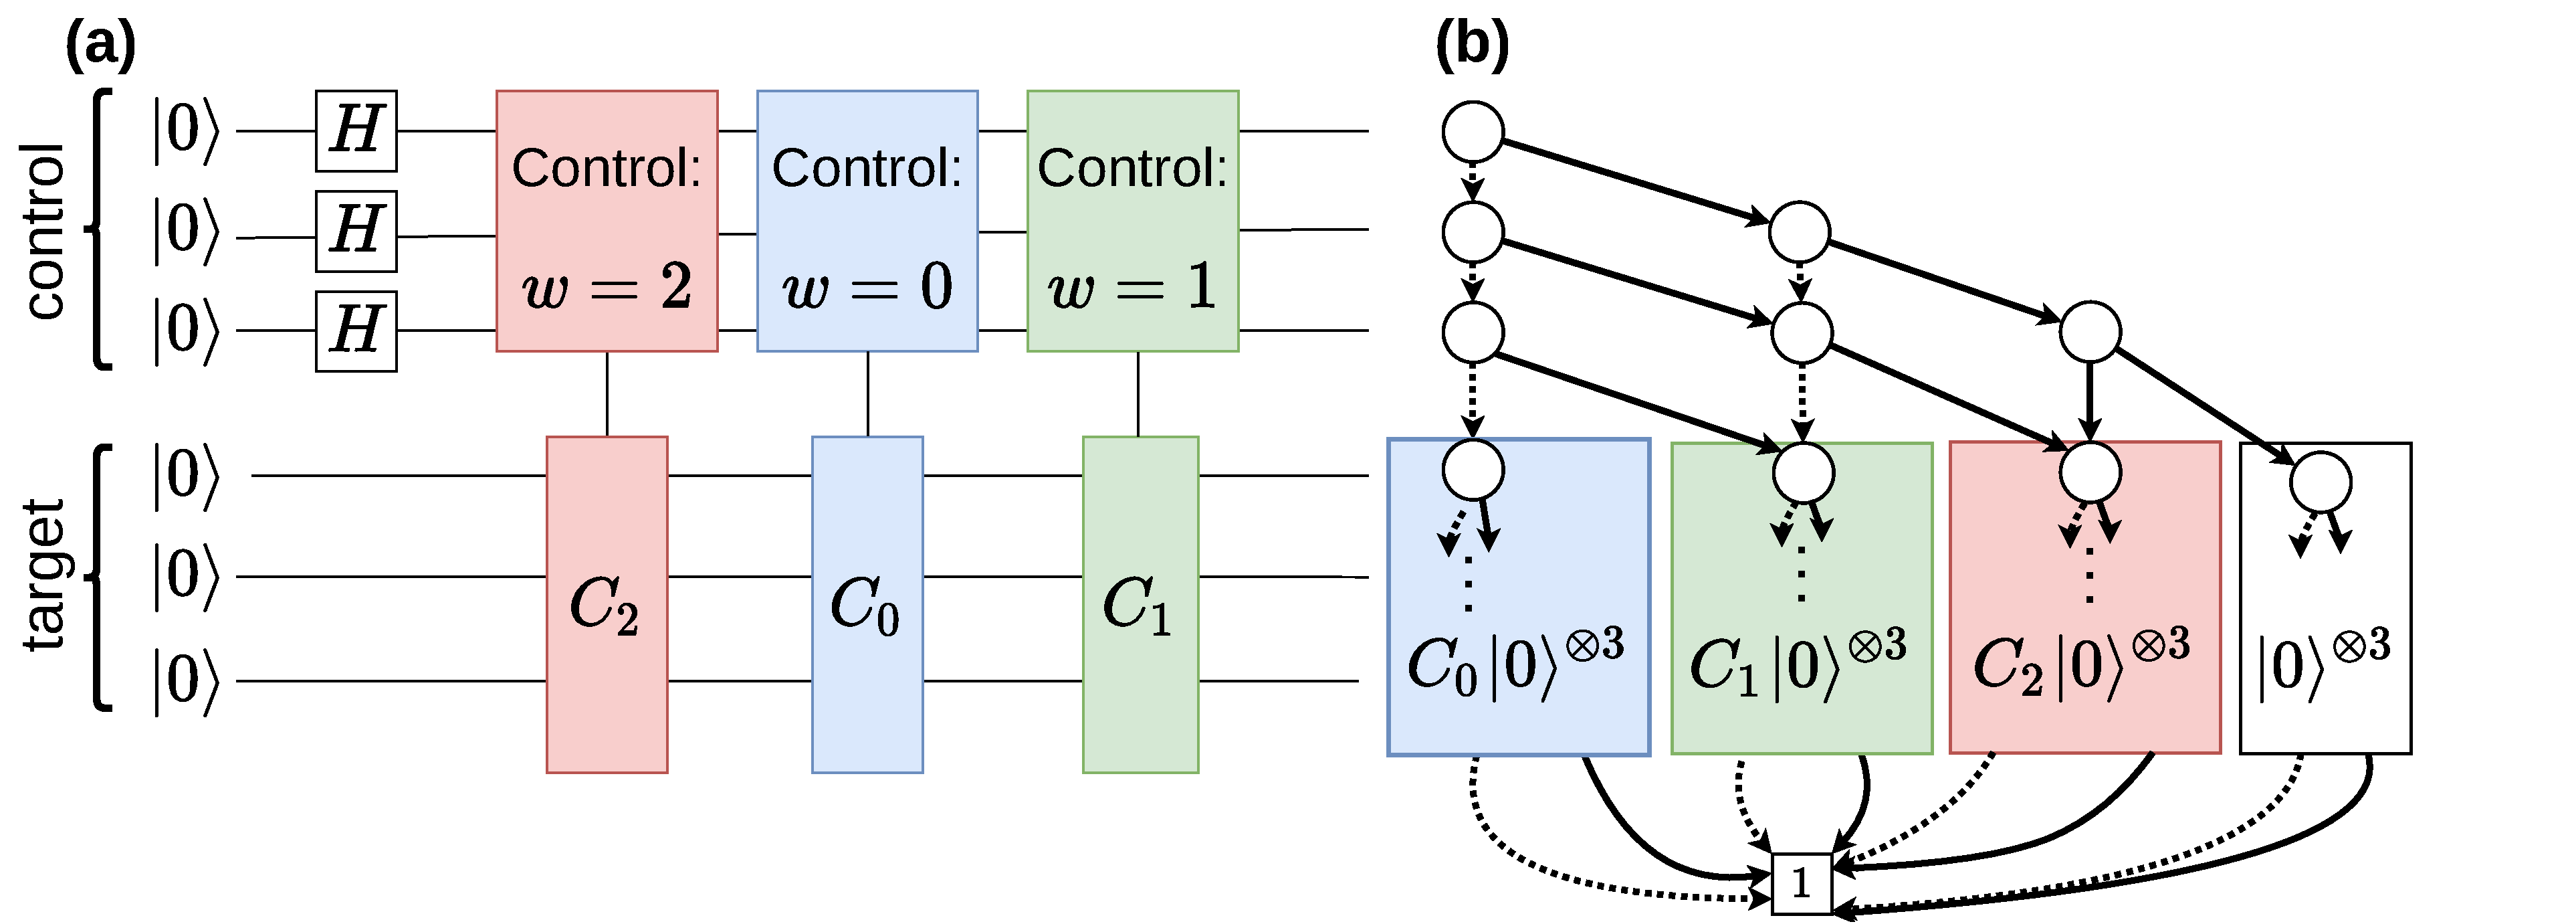
\includegraphics[width=\textwidth]{pics/weight-controlled-stabilizer-state-2.pdf}
	\caption{
        \textbf{(a)} A ``Hamming weight-controlled Clifford circuit'' on $3+3$ qubits with input state $\ket{0}^{\otimes 3} \otimes \ket{0}^{\otimes 3}$. 
        The depicted circuit consists of three controlled-Clifford gates, where the Clifford $C_w$ is only applied if the Hamming weight of the control register equals $w$ see also eq.~\eqref{eq:hamming-weight-control-gate}.
        \textbf{(b)} A Pauli-\limdd for the output state of the circuit in (a), where the colored blocks represent Pauli-\limdds for the states $C_w \ket{0}^{\otimes 3}$.
        The edges which originate in the control-register-part of the \limdd point to the top node of three different branches, each representing a constant Hamming weight of the control qubits (edge weights are all $\id$; recall dashed/solid lines represent low/high edges).
        The branch in the target-register-part corresponding to Hamming weight $w$ represents the state $C_w \ket{0}^{\otimes 3}$, which is a stabilizer state.
        We note that stabilizer states are represented by a polynomially-large \limdd (see \autoref{sec:exponential-separations}) while the width of the control-register-part of the \limdd can never exceed the possible number of Hamming weights on length-$n$ bitstrings, i.e. ${n \choose 2} = O(n^2)$.
        Consequently, Pauli-\limdds represent all Hamming weight-controlled Clifford circuits using only polynomially-many nodes.
    }
	\label{fig:weight-controlled-stabilizer-state}
\end{figure}

In order to investigate the hardness of HWC circuits for stabilizer rank methods, we employ the heuristic algorithm from \cite{bravyi2016trading} (explained in more detail in \cite{calpin2020exploring}) for searching for the stabilizer rank of Dicke states $\dicke{n}{w}$, which are equal superpositions of computational basis states with a given Hamming weight:
\[
    \dicke{n}{w} := \sum\limits_{\substack{x \in \{0, 1\}^n, \\|x| = w}} \ket{x}
    .
\]
To see that there exists HWC states $\ket{\phi}$ which have stabilizer rank $\chi(\ket{\phi})$ at least as large as the stabilizer rank $\chi(\dicke{n}{w})$of Dicke states, consider the HWC circuit consisting of the single gate $U_w^C$ where $C$ is the Pauli $X$ gate on the least significant qubit in the target register.
The resulting state is
\begin{equation}
    \label{eq:dicke}
    \ket{\phi} =
    \sum_{k=0,k\ne w}^n \dicke{n}{k}\otimes \ket{0}^{\otimes n} + \dicke{n}{w}\ket{0\ldots 01}
\end{equation}
By measuring the target register in the computational basis, the resulting control register state is $\dicke{n}{w}$ upon obtaining output $\ket{0\ldots 01}$.
Since computational-basis measurements cannot increase the stabilizer rank, we find $\chi(\ket{\phi}) \geq \chi(\dicke{n}{w})$.

\begin{table}[b!]
    \centering
    \setlength{\tabcolsep}{12pt}
    \begin{tabular}{|r|cccccc|}
        \hline
        & \multicolumn{6}{c|}{\textbf{Hamming weight $w$}}\\\hline
        \textbf{\#qubits $n$} & \textbf{0} & \textbf{1} & \textbf{2} & \textbf{3} & \textbf{4} & \textbf{5} \\\hline
        \textbf{1} & 1 &   &   &   &   &\\
        \textbf{2} & 1 & 1 &   &   &   &\\
        \textbf{3} & 1 & 2 &   &   &   &\\
        \textbf{4} & 1 & 2 & 2 &   &   &\\
        \textbf{5} & 1 & 3 & 2 &   &   &\\
        \textbf{6} & 1 & 3 & 4 & 2 &   &\\
        \textbf{7} & 1 & 4 & 7 & 4 &   &\\
        \textbf{8} & 1 & 4 & 8 & $\leq 11$  & 5 &\\
        \textbf{9} &   &   &   &   & & $>10?$  \\\hline
    \end{tabular}
    \caption{
        \label{table:stabilizer-rank-search}
        Heuristically-found upper bounds on the stabilizer rank $\chi$ of Dicke states $\dicke nw$ (eq.~\eqref{eq:dicke}) using the heuristic algorithm from Bravyi et al. \cite{bravyi2016trading} (see main text for details).
        Empty cells indicate non-existing or not-investigated states.
        In particular, we have not investigated $w> \lceil \frac{n}{2}\rceil$ since $\chi(\dicke{n}{w}) = \chi(\dicke{n}{n-w})$ because $X^{\otimes n} \dicke{n}{w} = \dicke{n}{n-w}$.
        For $\dicke{8}{3}$ and $\dicke{9}{5}$, we have run the heuristic algorithm to find sets of stabilizers up to size $11$ (theoretical upper bound) and $10$, respectively, but the algorithm has not found sets in which these two Dicke states could be decomposed.
        We emphasize that the algorithm is heuristic, so if there exists a stabilizer decomposition of a given rank, the algorithm might not find it.
    }
\end{table}

The heuristic algorithm follows a simulated-annealing approach: on input $n,w $ and $\chi$, it performs a random walk through sets of $\chi$ stabilizer states.
It starts with a random set $V$ of $\chi$ stabilizer states on $n$ qubits.
In a single `step', the algorithm picks one of these states $\ket{\psi} \in V$ at random, together with a random $n$-qubit Pauli operator $P$, and replaces the state $\ket{\psi}$ with $\ket{\psi'} := c(\id + P)\ket{\psi}$ with $c$ a normalization constant (or repeats if $\ket{\psi'} = 0$), yielding a new set $V'$.
The step is accepted with certainty if $F_V < F_{V'}$, where $F_V:= |\langle \dicke nw| \Pi_V \dicke{n}{w}|$ with $\Pi_V$ the projector on the subspace of the $n$-qubit Hilbert space spanned by the stabilizer states in $V$.
Otherwise, it is accepted with probability $\exp(-\beta (F_{V'} - F_V))$, where $\beta$ should be interpreted as the inverse temperature.
The algorithm terminates if it finds $F_V = 1$, implying that $\dicke{n}{w}$ can be written as linear combination of $V$, outputting the number $\chi$ as (upper bound to) the stabilizer rank.
For a fixed $\chi$, we use identical values to Bravyi et al. \cite{bravyi2016trading} and vary $\beta$ from $1$ to $4000$ in $100$ steps, performing $1000$ steps at each value of $\beta$.
%To determine the values of $\chi$ to investigate, we note the following two upper bounds to $\chi(\dicke{n}{w})$.
%First, following eq.~\eqref{eq:dicke}, $\dicke{n}{w}$ can be written as linear combination of ${n \choose w}$ computational-basis states so $\chi(\dicke{n}{w}) \leq {n \choose w}$.
%Second, $\dicke{n}{w} \propto \ket{0}\dicke{n-1}{w} + \ket{1}\dicke{n-1}{w-1}$, implying that we can use the sum of found upper bounds to the stabilizer ranks of $\dicke{n-1}{w}$ and $\dicke{n-1}{w-1}$ as an upper bound to $\chi(\dicke{n}{w})$.
%We ran the algorithm for $\chi$ ranging from $1$ up to the minimum of these two upper bounds.
See \cite{githubrepo} for our open-source implementation.

We provide the results of our numerical runs in \autoref{table:stabilizer-rank-search}.
Since our approach is based on using heuristic algorithms to find a good upper bound on the stabilizer rank, and not a lower bound, by construction we cannot guarantee any statement on the scaling of the rank itself.
Our approach could only have provided evidence that Dicke states do not have a rapidly scaling rank, thereby providing evidence that stabilizer-rank methods can simulate HWC states efficiently.
However, this is not what we observe, and our findings are consistent with the possibility that Dicke states have a superpolynomial rank.
Although further research is needed for a definitive answer, these numerics strengthen our confidence that \limdds can simulate HWC circuits faster than stabilizer-rank based methods.

%\section{Separation of LIMDD from known methods}
\label{sec:separation-discussion}

In the majority of this paper we have focused on the succinctness of quantum state representations in DD-based structures.
We finish off by analyzing the simulation power of Pauli-\limdds with respect to state-of-the-art quantum methods. i.e., those based on stabilizer rank~\cite{bravyi2019simulation}.
In order to establish a runtime separation, we are looking for a family of circuits that are efficiently simulatable by Pauli-\limdds, but that are not simulatable by stabilizer-rank methods or QMDDs.
For this discussion, recall that stabilizer-rank simulators require the circuits using Clifford gates only, and T-gates are implemented through gate teleportation~\cite{bravyi2019simulation}.
The resource for this are magic states, and overall efficacy of the simulation depends on the initial stabilizer rank representation of the input.

By simulation, we will mean the problem of sampling from a single chosen qubit in the Z (computational) basis, of a state generated by a quantum circuit (given as input) when applied to some simple fiducial state (e.g the all-zero state).
This is the weakest form of simulation. It should be noted however that the \limdd approach that we consider computes the final state explicitly by computing intermediate states applying gates in one by one fashion and therefore allows stronger forms of simulation.\todo{the strong form works in our favor. I mention this here} 
As additional constraint for \limdd/\qmdd, by `efficiently simulatable' we mean `produce poly-sized intermediary DDs with tractable operations'.

Our main finding is that fair comparison is difficult.
Our first example shows that, if we only allow direct simulation using stabilizer-rank simulation, it is trivial to produce circuit families where \limdds offer exponential speed-ups.
For a trivial example, consider Figure~\ref{fig:stabilizer-rank-hard}(a); if we simply consider the circuit comprising a layer of Hadamard gates, followed by a layer of $c$ T-gates, we end up in a setting where we require $\Omega(c^n)$ time for stabilizer rank-based simulators (the constant $c$ may depend on how well the n-fold product of magic states is decomposed in the stabilizer overcomplete basis, but it is widely believed that this is always exponential in $n$).
\todo{maybe replace Clifford part of circuit by hadamards?}
In contrast, the DT-\limdds perform the updates generating this state, represent and measure it efficiently. 
\todo{should argue! maybe can follow from in sec 5}

This example is of course unsatisfactory, as a quick glance reveals that, since we utilize only Z measurement(s), no tailing diagonal operators play a role in the final probabilities. In other words, the T-gate-tower can simply be ignored. 
This is a type of simple circuit rewrite which greatly extends the scope of stabilizer-rank simulator.

For a stronger example, consider replacing the T-gate tower by an interleaving of many T gates and gates which are diagonal in the computational basis.
in this case we cannot use identical arguments to simplify the circuit.
However, we can now note that any permutation matrix (w.r.t the computational basis) applied before a Z basis measurement can be executed in a post-processing step (it is just a re-labeling of the outputs). Combining this observation, with the irrelevance of diagonal operators, we see that we can ignore all permutation and phase gates before Z measurements. 

Clearly the story is more complicated if reasonable re-write and post processing rules are applied in the stabilizer-rank simulation.
Nonetheless, we have a number of examples of significantly more complex circuits, which involve linearly many T gates, even after the basic simplifications, meaning: removal of all tailing permutations and diagonal operators, and cancellation of all consecutive T-gates, within circuits.\todo{What happened to our empirical evidence? No longer relevant?}

The circuit family in Figure~\ref{fig:stabilizer-rank-hard}(b) is an example, containing many Toffoli gates~\cite{Toffoli} which each can be expressed as circuit of many T gates \todo{ref}.
It is the simplest family that we can come up that satisfying the above conditions.
As a sanity check, we proved that it is not a producing a stabilizer state.
\todo{still to do! ``Interestingly, we do this using LIMMQMDD methods (since it is not a tower IsoQMMD, this follows from canonicity in Th6 and Lemma 14). It is not simulatable by QMDD, since [add short argument]''}
We see that T gates appear in various controlled-Clifford operations, and not just in a strict layer of permutations and diagonal gates which can be resolved via post-processing we considered thus far, meaning simulation in the stabilizer rank formalism will not be efficient. 
\todo{VEDRAN: WAIT IS THIS TRUE? DOES THE BASIC REWRITE AS ABOVE NOT APPLY? PLEASE SANITY CHECK. I am worried this *again* talks about hardness of representing the state and not about hardness of output probabilities.... This is ok, but it still must be the case that we cannot apply the permutation-based and diagonal-absorption rules and get rid of all T gates that way}

One may wonder why not attempt a proof that no efficient rewrite process allows to construct equivalent efficient stabilizer-rank simulatable circuits.
This unfortunately would not be a meaningful request.
Since we consider only states which are efficiently processed by \limdd, we know there are efficient ways to simulate the circuits classically.
Consequently, if we allow \emph{all} possible rewrites, the re-write process can simply perform  \limdd-based simulation.

\todo[inline]{
Let us briefly consider the converse question of simulating stabilizer-rank-simulatable circuits in LIMQMDD.
[I DO NOT KNOW IF THE FOLLOWING IS TRUE]; Poly-sized superpositions of stabilizer states are efficiently representable in  LIMQMDD, and Clifford updates are efficient (except the Hadamard, which we perform using the mapping through the stabilizer, although other options are conceivable). 
Consequently simulation which keeps stabilizer rank low, is simulatable in our LIMQMDD as well. 
}




\begin{figure}
	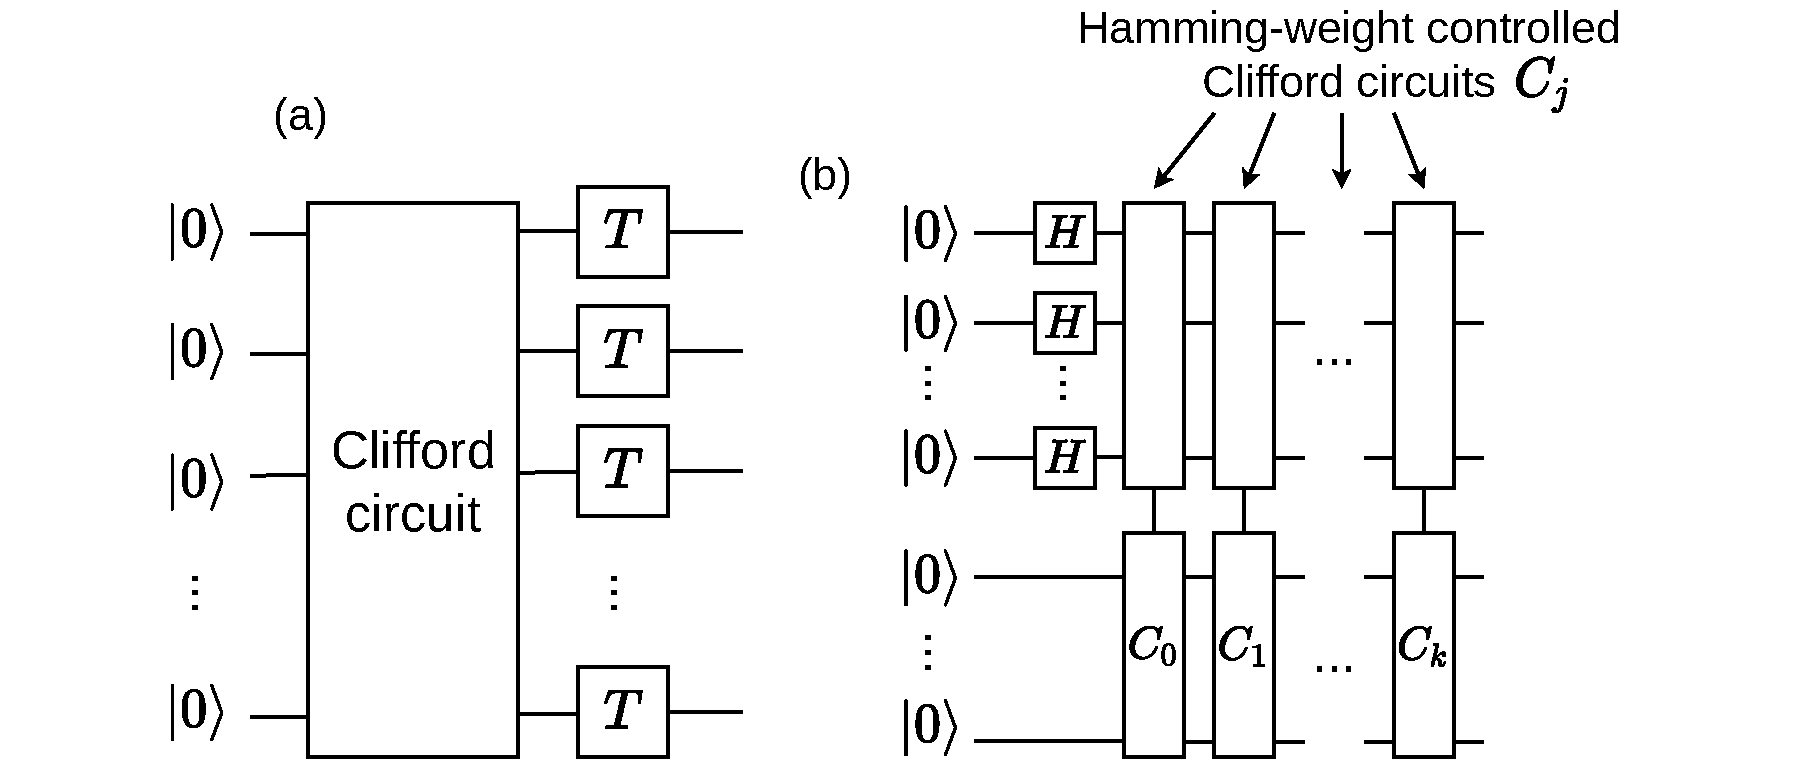
\includegraphics[width=1.0\textwidth]{pics/t-gate-tower.pdf}
	\caption{
		Circuits output a polynomially-size \limdd.
		For (b), the Hamming-weight controlled-$C$ gate on $c$ control qubits and $t$ target qubits maps $\ket{x}\otimes \ket{y}$ to $\ket{x}\otimes C\ket{y}$ if $|x| = 1$ and to $\ket{x}\otimes\ket{y}$ otherwise, for $x\in \{0, 1\}^c$ and $y\in \{0, 1\}^t$.
		Here, $|x| = \sum_{j=1}^c x_j$ denotes the Hamming weight of $x$.
		\todo[inline]{need to explain how to implement Hamming-weight controlled gate?}
		\label{fig:stabilizer-rank-hard}
	}
\end{figure}



%\input{sections/iso_qmmd_measurement.tex}
%\input{sections/related_work.tex}
\section{Discussion \label{sec:discussion}}

We have introduced \limdd, a novel decision diagram-based method to simulate quantum circuits, which enables polynomial-size representation of a strict superset of stabilizer states and of the states represented by polynomially-large \qmdds.
To prove this, we have shown the first lower bounds on the size of \qmdds for stabilizer states:
they are exponential-size for certain families of stabilizer states.
\limdds achieve a more succinct representation by representing states up to 
local invertible maps which uses single qubit (local) operations from a group $G$.
We have investigated the choices $G=\pauli$, $G=\braket{Z}$ and $G=\braket{X}$,
and found that any choice suffices for an exponential advantage over \qmdds;
notably, the choice $G=\pauli$ allows us to succinctly represent stabilizer states.
We also defined reduction rules for Pauli-\limdd and showed that for each set of 
quantum states which are equivalent under local Pauli operations,
modulo normalization factor, has a unique reduced Pauli-\limdd as representative.

Furthermore, we showed how to simulate arbitrary quantum circuits, encoded as Pauli-\limdds.
The resulting algorithms are often faster than for \qmdds.
In contrast to \qmdds, Clifford circuits (initialized to $\ket{0}$)
can be simulated by Pauli-\limdds in polynomial time.
This in itself is not an interesting feat, since efficient simulation methods for
the stabilizer regime have been known since the Gottesman-Knill theorem.
However, we also showed that Pauli-\limdds can efficiently simulate
a circuit family we call Hamming weight-controlled Clifford circuits.
And we provide empirical evidence that these circuits are hard for stabilizer-rank
based simulation methods.
%we were strengthened in this exception by exploratory numerics.

An obvious next step is to investigate other choices for $G$.
Of interest are both the representational capabilities of such diagrams
(do they represent interesting states?), and the algorithmic capabilities
(can we still find efficient algorithms which make use of these diagrams?).
In this vein, an important question is what the relationship is between \glimdds
(for various choices of $G$) and existing formalisms for the classical simulation of quantum circuits, such as those based on match-gates~\cite{terhal2001classical,jozsa2008matchgates,hebenstreit2020computational} and tensor networks~\cite{orus2014practical}.
It would also be interesting to compare \limdds to graphical depictions of quantum computation, 
following similar work for \qmdds~\cite{vilmart2021quantum}.
We leave empirical evaluations into the consequences of \limdd methods for efficient
quantum circuit simulation, for future work. This would obviously include a 
comparison with stabilizer rank simulation~\cite{bravyi2019simulation}.

Finally, we note that the current definition of \limdd imposes a strict total order
over the qubits along every path from root to leaf.
It is known that the chosen order can greatly influence the size of the DD~\cite{rudell1993dynamic,wegener2000branching},
making it interesting to investigate variants of \limdds with a flexible ordering.


%\input{sections/decision_diagrams.tex}
%\input{sections/from_compendium.tex}


\bibliography{lit}

\appendix
% Some of these appendices are commented out only for faster compilation


\newpage
\section{Proof that cluster states need exponentially-large QMDDs}
\label{sec:graph-state-lower-bound}


In this appendix, we formally prove that cluster states have exponential size in \qmdds \autoref{thm:graph-state-qmdd-lower-bound}.
We first fix notation and definitions, after which we prove 
%\autoref{thm:graph-state-qmdd-lower-bound} 
the theorem using two lemmas.

Let $G$ be an undirected graph with vertices $V_G=\{v_1, \dots, v_n\}$ and edge set $E_G \subseteq V_G\times V_G$.
For a subset of vertices $S\subseteq V_G$, the $S$-induced subgraph of $G$ has vertices $S$ and edge set $(S \times S) \cap E$.
Given $G$, its graph state $\ket{G}$ is given in \autoref{eq:graph-state-definition} in \autoref{sec:preliminaries} and can equivalently be expressed as
\[
    \ket{G} = \sum_{\vec x\in \set{0,1}^n} (-1)^{f_G(\vec x) } \ket{\vec x}
\]
where $f_G(\vec{x})$ is the number of edges in the $S$-induced subgraph of $G$.

For a function $f: \{0, 1\}^n \rightarrow \mathbb{C}$ and bit string $\vec a=a_1\cdots a_k\in\{0, 1\}^k$, we denote by $f_{\vec{a}}$ the subfunction of $f$ restricted to $\vec a$:
\begin{align}
f_{\vec a}(x_{k+1},\ldots, x_n) := f(a_1,\ldots, a_k,x_{k+1},\ldots, x_n)
\end{align}
We also say that $f_{\vec a}$ is a subfunction of $f$ of \emph{order} $|\vec a|=k$.
%The string $a$ is called a \emph{partial assignment} to $f$.

We will also need the notions of boundary and strong matching.

\begin{definition}[Boundary]
	For a set $S\subseteq V_G$ of vertices in $G$, the \emph{boundary} of $S$ is the set of vertices in $S$ adjacent to a vertex outside of $S$.
\end{definition}

\begin{definition}[Strong Matching]\label{def:smatch}
	Let $G=(V,E)$ be an undirected graph. A \emph{strong matching} is a
	subset of edges $M \subseteq E$ that do not share any vertices (i.e., it is a matching)
	and no two edges of $M$ are incident to the same edge of $G$, i.e.,
	an edge in $E \setminus M$. Alternatively, a strong matching is a matching $M$ s.t. $G[V(M)] = M$.
	We say that $M$ is an $(S,T)$-strong matching for two sets of vertices $S,T\subset V$ if $M\subseteq S\times T$.
	For a strong matching $M$ and a vertex $v\in V(M)$, we let $M(v)$ denote the unique vertex to which $v$ is matched by $M$.
\end{definition}



%\todo[inline]{
% Write $\chi(x_1, \dots, x_n)$
%be the indicator function for vertices: $\chi(x_1, \dots, x_n) \defn \{v_i \mid x_i=1, i \in [n]\} $.
%Let $f_G\colon \bool^n\to \bool$ be the number of edges in the $S$-induced subgraph of $G$, written $G[S]$, modulo $2$, as in \autoref{eq:induced-subgraph-fn}. 
%\begin{align}
%	\label{eq:induced-subgraph-fn}
%	f_G(x_1,\ldots, x_n)  \defn |G[ \chi(x_1, \dots, x_n)]|\mod 2
%\end{align}
%%Here $E[S]$ is the subgraph induced by the set indicated by the vertices $S \subseteq V$.
%For a graph $G$, the graph state $\ket{\psi_G}$ is defined in terms of $f_G$, namely,
%\begin{align} 
%	\ket{\psi_G} \defn \sum_{\vec x\in \set{0,1}^n} (-1)^{f_G(\vec x) } \ket{\vec x}
%\end{align}
%Then the main result is \autoref{th:graph-state-qmdd-lower-bound}: that the function $f_G$ is difficult for BDDs, and $\ket{\psi_G}$ is difficult for \textsc{QMDD}s.
%}
%
%Given a variable order, a Decision Diagram (DD) is a DAG that uniquely represents a function (see \autoref{sec:preliminaries-dd} for details).
%Each path in a DD represents a (partial) assignment to the first variables
%in the order. 
%We prove \autoref{th:graph-state-qmdd-lower-bound} by counting unique subfunctions (= different DD nodes) induced by
%those partial assignments (for any variable order).
%\autoref{thm:bdd-size-from-subfunctions} and \autoref{thm:qmdd-size-from-subfunctions} show how we translate our count of unique subfunctions to a lower bound on diagram size.

Using these definitions and notation, we prove \autoref{thm:graph-state-qmdd-lower-bound}.

\begin{proof}[Proof of \autoref{thm:graph-state-qmdd-lower-bound}]
%	Consider the set $B_S:=\text{Boundary}(S)$.
%	
Let $G=\text{lattice}(n,n)$ be the undirected graph of the $n\times n$ lattice,
with vertex set $V=\{v_1,\ldots, v_{n^2}\}$.
Let $\sigma=v_1v_2\cdots v_{n^2}$ be a variable order, and let $S=\{v_1,v_2,\ldots, v_{\frac{1}{2}n^2}\}\subset V$ be the first $\half n^2$ vertices in this order.

The proof proceeds broadly as follows.
First, in \autoref{thm:strong-matchings-yield-subfunctions}, we show that any $(S,\overline S)$-strong matching $M$ effects $2^{|M|}$ different subfunctions of $f_G$.
Second, \autoref{thm:large-strong-matching} shows that the lattice contains a large $(S,\overline S)$-strong matching for any choice of $S$.
    Put together, this will prove the lower bound on the number of QMDD nodes as in \autoref{thm:graph-state-qmdd-lower-bound} by the fact that a QMDD for the grid graph state $G$ has a node per unique subfunction of the function $f_G$.
	Figure \ref{fig:strong-matching-in-grid} illustrates this setup for the $5\times 5$ lattice.

\begin{lemma}
	\label{thm:strong-matchings-yield-subfunctions}
	Let $M$ be a non-empty $(S,\overline S)$-strong matching for the vertex set $S$ chosen above.
	If $\sigma=v_1v_2\cdots v_{n^2}$ is a variable order where all vertices in $S$ appear before all vertices in $\overline S$, then $f_G(x_1,\ldots, x_{n^2})$ has $2^{|M|}$ different subfunctions of order $|S|$.
\end{lemma}
\begin{proof}
	Let $S_M:=S\cap V(M)$ and $\overline S_M:=\overline S\cap M$ be the sets of vertices that are involved in the strong matching.
Write $\chi(x_1, \dots, x_n)$ for the indicator function for vertices: $\chi(x_1, \dots, x_n) := \{v_i \mid x_i=1, i \in [n]\} $.
	Choose two different subsets $A,B\subseteq S_M$ and let $\vec{a}=\chi^{-1}(A)$ and $\vec{b}=\chi^{-1}(B)$ be the corresponding length-$|S|$ bit strings.
	%		We will show that $\vec{a}$ and $\vec{b}$ induce different subfunctions.
	%		Let $\vec{a}=a_1,\ldots,a_{\half n^2}$ and $\vec{b}=b_1,\ldots,b_{\half n^2}$ be two different partial assignments which are nonzero only on $S_M$, i.e., for all $v_i\not\in S_M$, $a_i=b_i=0$.
	%		The bit strings correspond to sets $S_{\vec a},S_{\vec b}\subseteq S_M$.
	%		
	These two strings induce the two subfunctions $f_{G,\vec{a}}$ and $f_{G,\vec{b}}$.
	We will show that these subfunctions differ in at least one point.
	
	First, if $f_{G,\vec{a}}(0,\ldots, 0)\ne f_{G,\vec{b}}(0,\ldots, 0)$, then we are done.
	Otherwise, take a vertex $s\in A\oplus B$
    and say w.l.o.g. that $s\in A\setminus B$.
	Let $t=M(s)$ be its partner in the strong matching.
	Then we have, $|E[A\cup \{t\}]| = |E[A]|+1$ but $|E[B\cup \{t\}]|=|E[B]|$.
	Therefore we have 
	%		Then we have 
	\begin{align}
	f_{G,\vec a}(0,\ldots, 0, x_t=0, 0,\ldots, 0) ~~\ne~~ &f_{G,\vec a}(0,\ldots,0,x_t=1,0,\ldots, 0) \\
	f_{G,\vec b}(0,\ldots, 0, x_t=0, 0,\ldots, 0) ~~=~~ & f_{G,\vec b}(0,\ldots, 0,x_t=1,0,\ldots, 0)
	\end{align}
	%		This is because the edge $(s,t)$ is counted in the $\vec a$ subfunction, but not in the $\vec b$ subfunction.
	%		
	We see that each subset of $S_M$ corresponds to a different subfunction of $f_G$. Since there are $2^{|M|}$ subsets of $M$, $f_G$ has at least that many subfunctions.
\end{proof}

We now show that the $n\times n$ lattice contains a large enough strong matching.

\begin{lemma}
	\label{thm:large-strong-matching}
	Let $S=\{v_1,\ldots, v_{\frac{1}{2} n^2}\}$ be a set of $\half n^2$ vertices of the $n\times n$ lattice, as above.
	Then the graph contains a $(S,\overline S)$-strong matching of size at least $\floor{\frac{1}{12}n}$.
\end{lemma}
\begin{proof}
	Consider the boundary $B_S$ of $S$.
	This set contains at least $n/3$ vertices, by Theorem 11 in \cite{lipton1979generalized}.
	Each vertex of the boundary of $S$ has degree at most $4$. 
    It follows that there is a set of $\left\lfloor \frac{1}{4}|B_S|\right\rfloor$ vertices which share no neighbors.
	% todo B_T or \overline S?
	In particular, there is a set of $\left\lfloor \frac{1}{4}|B_S| \right\rfloor\geq \floor{\frac{1}{12}n}$ vertices in $B_S$ which share no neighbors in $\overline S$.
\end{proof}
Put together, every choice of half the vertices in the lattice yields a set with a boundary of at least $n/3$ nodes, which yields a strong matching of at least $\floor{\frac{1}{12}n}$ edges, which shows that $f_G$ has at least $2^{\floor{\frac{1}{12}n}}$ subfunctions of order $\frac{1}{2}n^2$.
\end{proof}

\begin{figure}[h!]
\centering
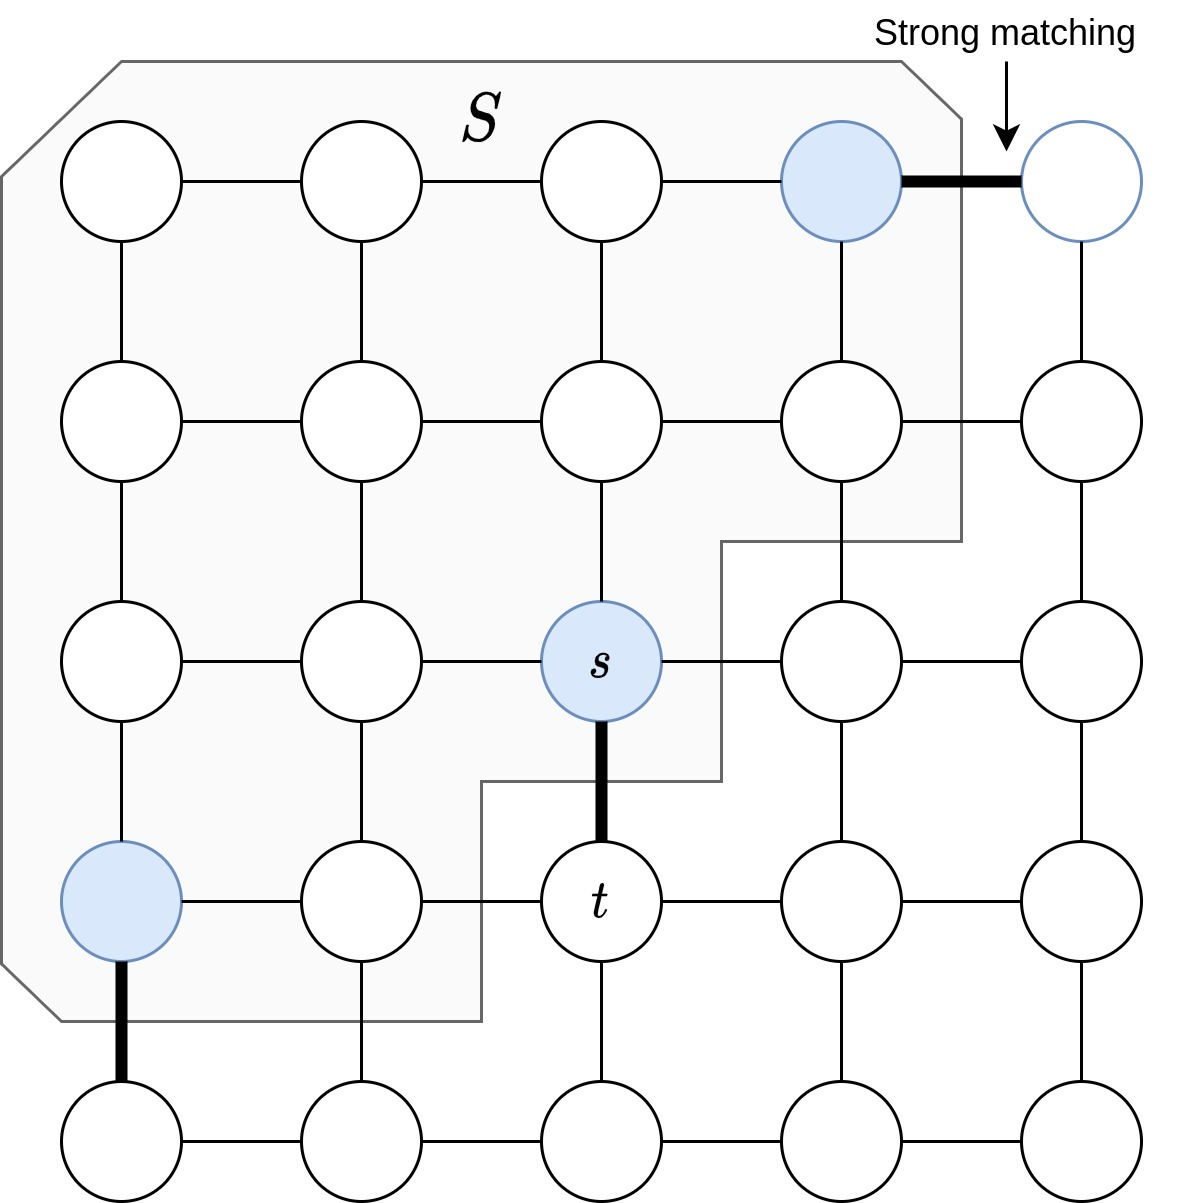
\includegraphics[width=0.45\textwidth]{pics/strong-matching-in-grid.jpg}
\caption{
    The $5\times 5$ grid graph, partitioned in a vertex set $S$ and its complement $\overline{S}$.
    A strong matching between $S$ and $\overline{S}$ is indicated by black edges.
}
\label{fig:strong-matching-in-grid}
\end{figure}


% todo =======================

\subsection{Proof that XOR states need exponentially large QMDDs}

We now show that \qmdds which represent so-called XOR states are exponentially large in the worst case.
On the other hand, in \autoref{sec:graph-states-limdds}, we will show that these states can be represented using only $\mathcal O(n)$ nodes by $\braket{X}$-\limdds, showing that they are exponentially more succinct than \qmdds.
We define XOR states as uniform superpositions over vectors spaces, as follows.

\begin{definition}[XOR-state]
	\label{def:xor-states}
	Let $V\subseteq\{0,1\}^n$ be a vector space, i.e., for every $x,y\in V$ it holds that $x\oplus y\in V$.
	Then the XOR-state $\ket{V}$ is the uniform superposition over the elements of $V$, i.e.,
	\begin{align}
	\ket{V}=\frac{1}{\sqrt{|V|}}\sum_{x\in V}\ket x
	\end{align}
\end{definition}

%The normalization factor $1/\sqrt{|V|}$ is not important to us, because our diagrams do not necessarily normalize a quantum state.
We will use the following result by \v{D}uri\v{s} et al. on binary decision diagrams (\bdds), which are \adds with codomain $\{0, 1\}$.
%The \qmdd lower bound is a corollary to the following result by \v{D}uri\v{s} et al. on binary decision diagrams (\textsf{BDD}s), which are \adds with codomain $\{0, 1\}$.

\begin{theorem}[\v{D}uri\v{s} et al.\cite{vdurivs2004multi}]
	\label{thm:random-vector-space-hard-for-bdd}
	The characteristic function $f_V: \{0, 1\}^n \rightarrow \{0, 1\}$ of a randomly chosen vector space $V$ in $\{0, 1\}^n$, defined as $f_V(x)=1$ if $x\in V$ and  $0$ otherwise, needs a \bdd of size $2^{\Omega(n)}/(2n)$ with high probability.
	%    \todo[inline]{@Lieuwe: should define branching program. Can replace by BDD?}
\end{theorem}

Our result follows by noting that if $f$ is as above, or indeed if $f$ is any function with codomain $\{0, \lambda\}$ for any scalar $\lambda$, then the \qmdd of the state $\ket{f}=\sum_xf(x)\ket{x}$ has the same structure as the \bdd of $f$.
That is to say, in this case, the \bdd and \qmdd are graphs with the same number of nodes.

\begin{corollary}
	\label{thm:random-xor-state-hard-for-qmdd}
	For a random vector space $V\subseteq \{0,1\}^n$, the XOR-state $\ket{V}$ requires \qmdds of size $2^{\Omega(n)}/(2n)$ with high probability.
\end{corollary}
\begin{proof}
	A \bdd encodes a function $f\colon \{0,1\}^n\to\{0,1\}$.
	In this case, the \bdd encodes $f_V$, the characteristic function of $V$.
	A \bdd is a graph which contains one node for each subfunction of $f$.
	
	Similarly, a \qmdd representing a state $\ket{\phi}=\sum_xf(x)\ket{x}$ can be said to represent the function $f\colon\{0,1\}^n\to\mathbb C$, and contains one node for each subfunction of $f$ modulo scalars.
	In this case, it represents the function $1/\sqrt{|V|}f_V\colon \{0,1\}^n\to\{0,1/\sqrt{|V|}\}$.
	However, in the case of $f_V$, two distinct subfunctions are not equal up to a scalar, because the codomain is $\{0,1\}$.
	To this end, let $f_{V,a},f_{V,b}$ be distinct subfunctions of $f_V$ induced by partial assignments $a,b\in\{0,1\}^k$.
	We will show that there is no $\lambda\in\mathbb C^{\ast}$ such that $f_{V,a}=\lambda f_{V,b}$.
	To see this, say that the two subfunctions differ in the point $x\in\{0,1\}^{n-k}$, i.e., $f_{V,a}(x)\ne f_{V,b}(x)$.
	Say without loss of generality that $f_{V,a}(x)=0$ and $f_{V,b}(x)=1$.
	Then, since $\lambda\ne 0$, we have $\lambda=\lambda f_{S,b}(x)\ne f_{V,a}(x)=0$, so $f_{V,a}\ne \lambda f_{B,b}$.
	
	Because distinct subfunctions of $f_V$ are not equal up to a scalar, the \qmdd for $\ket{V}$ contains a node for every subfunction of $f_V$.
	We conclude that, since by \autoref{thm:random-vector-space-hard-for-bdd} with high probability the \bdd representing $f_V$ has exponentially many nodes, so does the \qmdd representing $\ket{V}$.
\end{proof}
\section{How to write graph states, XOR-states and stabilizer states as Tower-\limdds}
\label{sec:graph-states-limdds}
\label{sec:proof-stabilizer-states-tower-limdds}
%\todo[inline]{Tim: should add `semi-reduced' to all three theorems? (even though this is only properly defined in the context of Pauli-\limdds?)}
%\todo[inline]{Tim: not yet made domain notation correct, e.g. make all Pauli strings represented by $P, Q$, etc.}

In this appendix, we prove that the families of $\langle Z\rangle$-, 
$\langle X\rangle$-, and Pauli-Tower-\limdds correspond to graph states, XOR states (see \autoref{def:xor-states} below), and stabilizer states, respectively, in \autoref{thm:graph-states-z-limdd}, \autoref{lemma:vector-space-x-limdd} and \autoref{thm:pauli-tower-limdds-are-stabilizer-states} below.
\autoref{def:reduced-limdd} for reduced \Pauli-\limdds also holds when exchanging \Pauli{} with $\bracket{X}$. However, it does not work for $\bracket{Z}$ by \ref{obs:subgroups}. Note however, that our proofs do not rely on the reduced definition, but on \autoref{def:limdd}.


We recall that a Tower-\limdd representing an $n$-qubit state is a \limdd which has, besides the leaf, $n$ nodes.
%Graph states and XOR states are stabilizer states, so they can be succintly represented by a generating set of their stabilizer groups.
%Our proofs are constructive: given the generating set for a graph state/XOR state/stabilizer state, we construct the state's $\langle Z \rangle$-/$\langle X\rangle$-/$\Pauli$-Tower-\limdds in polynomial time in the number of qubits.

\begin{proposition}[Graph states are $\langle Z\rangle$-Tower-\limdds]
    \label{thm:graph-states-z-limdd}
    Let $n\geq 1$.
    Denote by $\mathcal{G}_n$ the set of $n$-qubit graph states and write $\mathcal{Z}_n$ for the set of $n$-qubit quantum states which are represented by Tower-\limdds which low-edge-labels $\id$ and high-edge labels $\lambda \bigotimes_j P_j$ with $P_j \in \{\id[2], Z\}$ and $\lambda \in \{0, 1\}$.
    Then $\mathcal{G}_n = \mathcal{Z}_n$.
\end{proposition}
\begin{proof}
    We establish $\mathcal{G}_n \subseteq \mathcal{Z}_n$ by providing a procedure to convert any graph state in $\mathcal{G}_n$ to a reduced Tower-\limdd in $\mathcal{Z}_n$.
	See \autoref{fig:graph-state-as-line-iso-qmdd} for an example of a $4$-qubit graph state.
	
	\textbf{Base case: $n=1$.} We note that there is only one single-qubit graph state by definition (see \autoref{eq:graph-state-definition}), which is \mbox{$\ket{+} := (\ket{0} + \ket{1}) / \sqrt{2}$} and can be represented as \limdd by a single node (in addition to the leaf node): see \autoref{fig:graph-state-as-line-iso-qmdd}(a).
	
	\textbf{Induction case.}For the inductive step, we consider an $(n+1)$-qubit graph state $\ket{G}$ corresponding to the graph~$G$.
	We isolate the $(n+1)$-th qubit by decomposing the full state definition from  \autoref{eq:graph-state-definition} according to \autoref{eq:quantum-state-recursive}:
	\begin{equation}
	% Overweeg: 
        \ket{G} = 
        \frac{1}{\sqrt{2}}\left(\ket{0} \otimes \ket{G_{1..n}} + \ket{1} \otimes 
            \underset{\textnormal{Isomorphism B}}{ \underbrace{
\left[
            \bigotimes_{(n+1,j)\in E} Z_j
            \right] 
            }}
        \ket{G_{1..n}}\right)
		\label{eq:graph-state-induction}
	\end{equation}
where $E$ is the edge set of $G$ and $G_{1..n}$ is the induced subgraph of $G$ on vertices $1$ to $n$.
Thus, $\ket{G_{1..n}}$ is an $n$-qubit graph state on qubits 1 to $n$.
% Can be represented as <<a>> line-like \limdd
    Since $\ket{G_{1..n}}$ is a graph state on $n$ qubits, by the induction hypothesis, we have a procedure to convert it to a Tower-\limdd $\in \mathcal{Z}_{n-1}$.
Now we construct a Tower-\limdd for $\ket{G}$ as follows.
The root node has two outgoing edges, both going to the node representing $\ket{G_{1.. n}}$.
    The node's low edge is labeled with $\mathbb I$, and the node's high edge is labeled $B=0$ if the $(n+1)$-th qubit is isolated, and otherwise with 
\begin{align}
	B = \bigotimes_{(n+1,j)\in E}Z_j
\end{align}
Thus the root node represents the state $\ket{0}\ket{G_{1..n}}+\ket{1}B\ket{G_{1..n}}$, satisfying \autoref{eq:graph-state-induction}.
\begin{figure*}
    \begin{centering}
    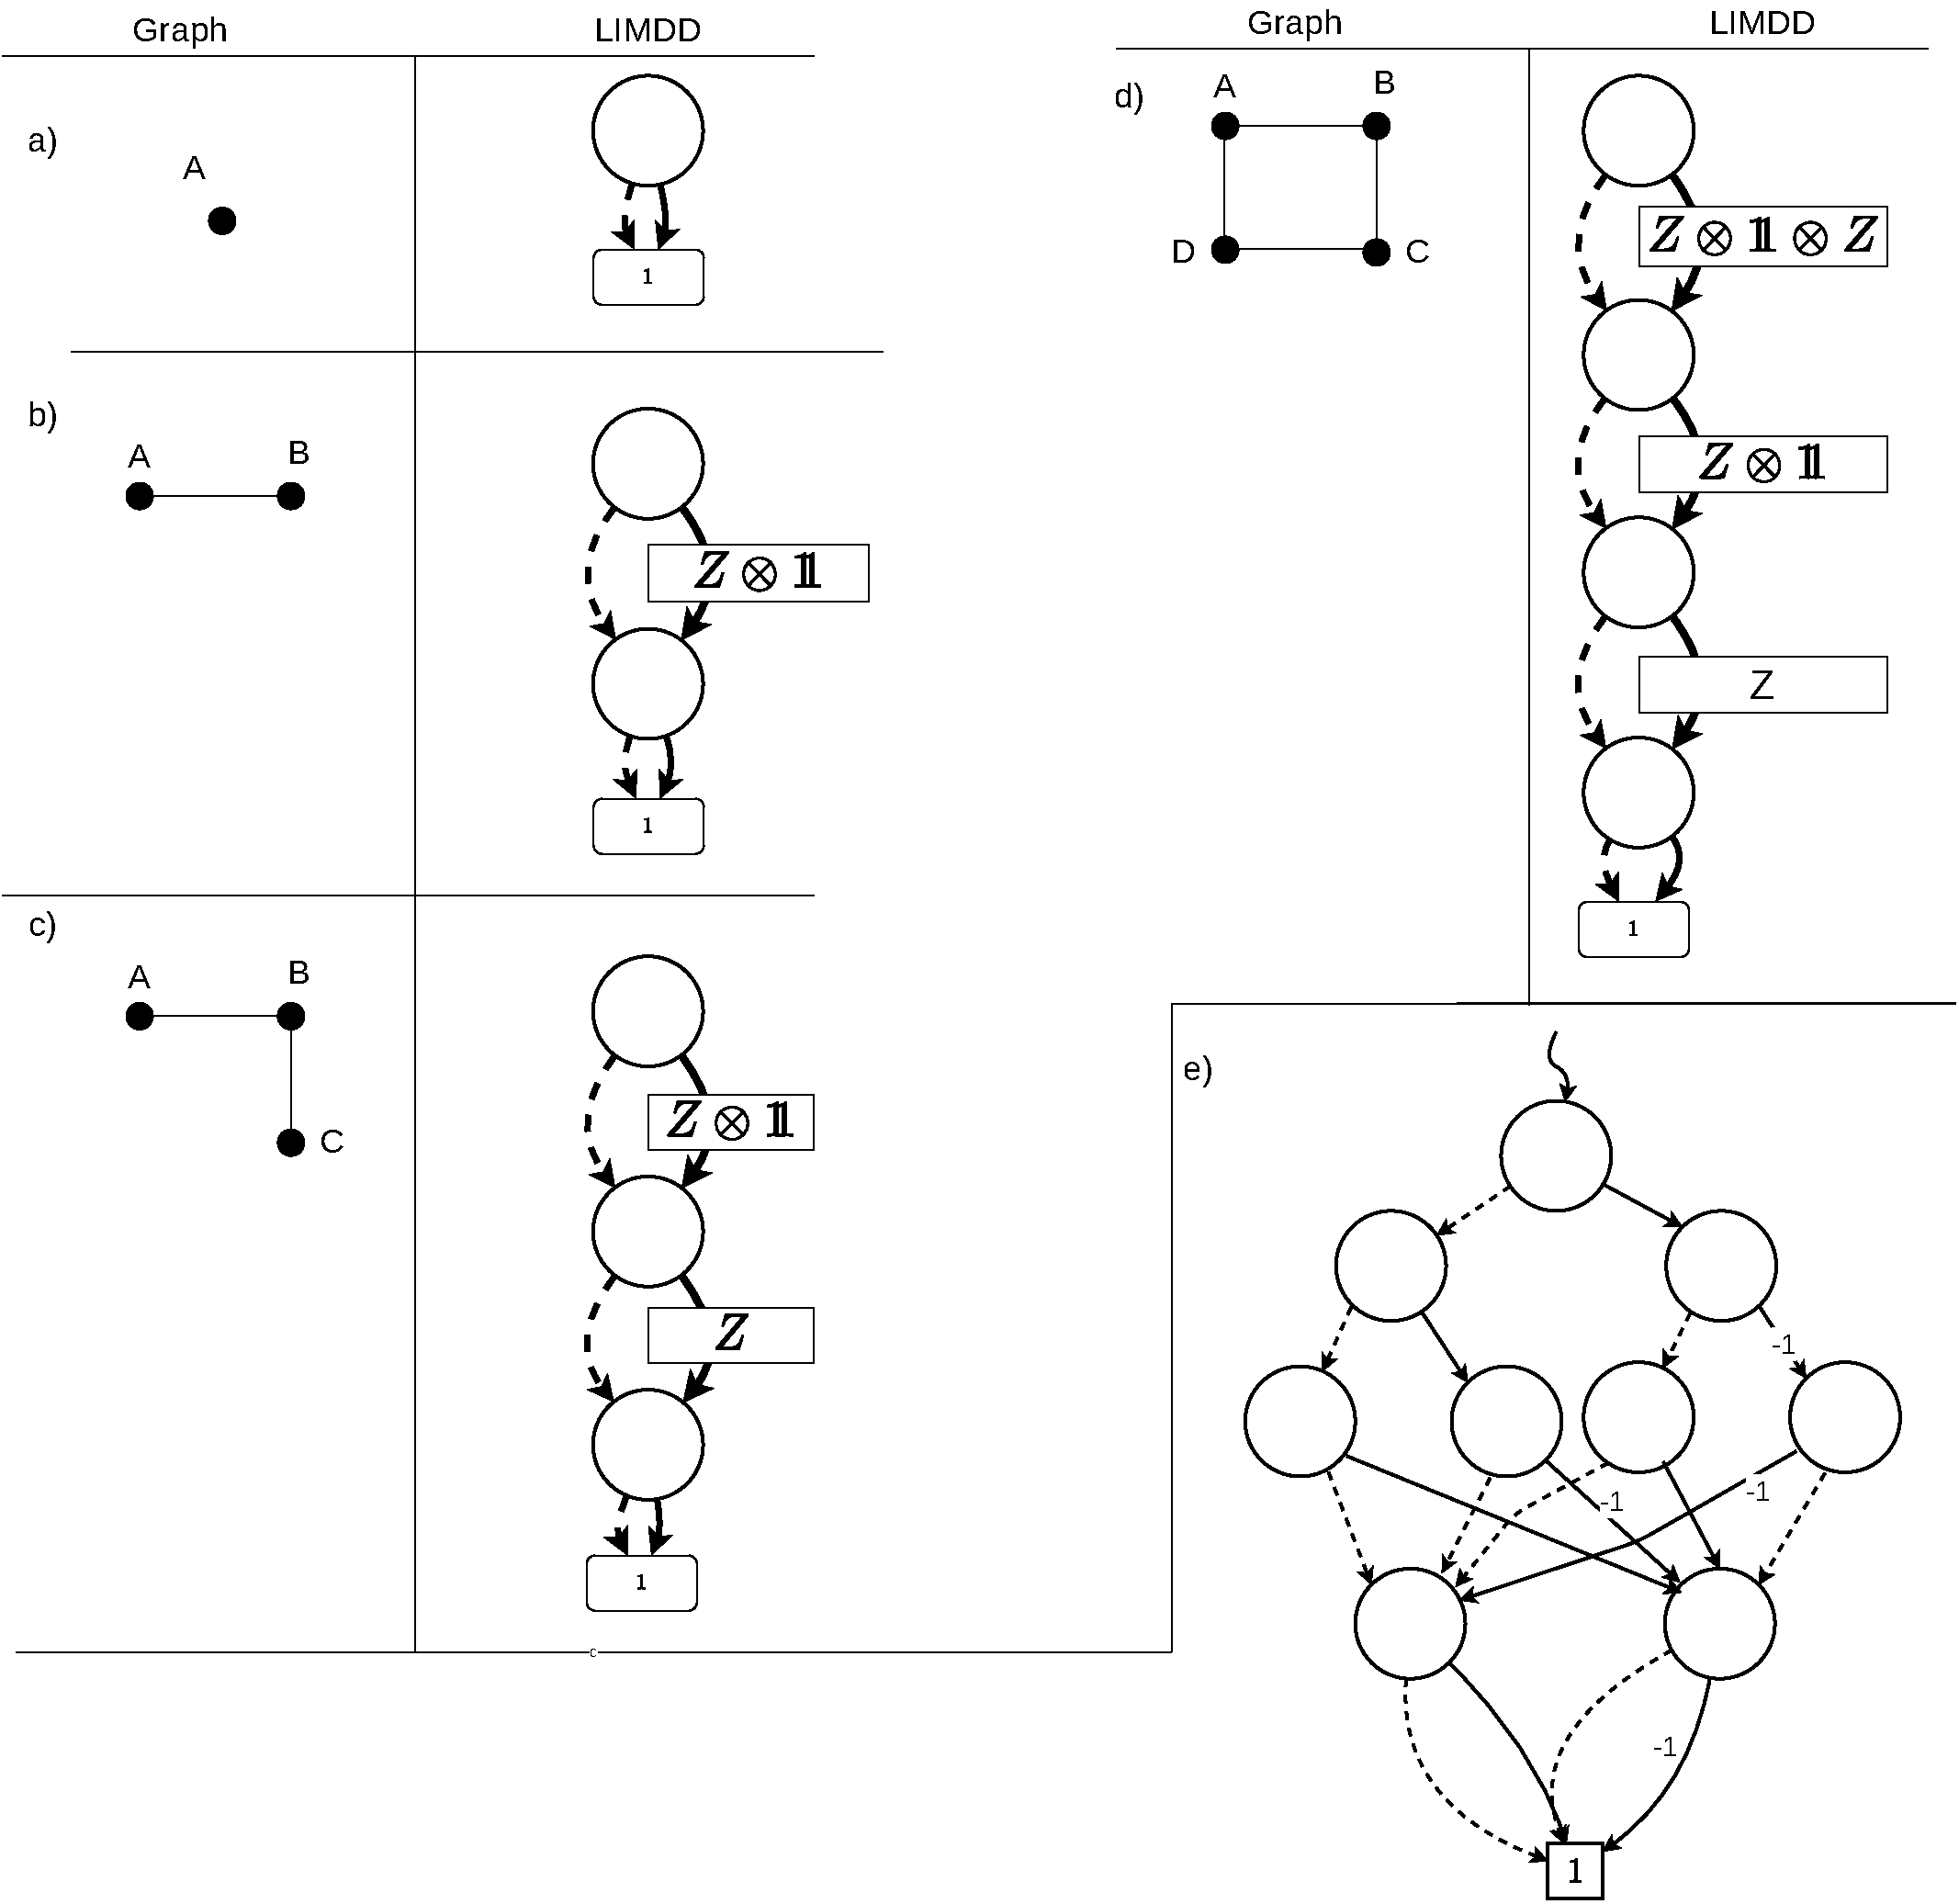
\includegraphics[width=1.0\textwidth]{pics/graph-state-construction.pdf}
	\caption{
		Construction of the Tower-\limdd for the 4-qubit cluster graph state, by iterating over the number of vertices in the graph.
    (a) First, we consider the single-qubit graph state, which corresponds to a the subgraph containing only vertex $A$.
    (b) Then, we add vertex $B$, which is connected to $A$ by an edge.
	The resulting \limdd is constructed from the \limdd from (a) by adding a new root node and an isomorphism node.
	The isomorphism is $\unit_A \otimes Z_B$, since vertex $C$ is connected to vertex $B$ (yielding the $Z$ operator) but not to $A$ (yielding the identity operator $\unit$).
    This process is repeated for a third vertex $C$ (c) until we reach the \limdd of the full 4-qubit cluster graph state (d).
	For comparison, (e) depicts a QMDD for the same graph state, which has width 4 instead of 1 for the \limdd.
		\label{fig:graph-state-as-line-iso-qmdd}
		}
    \end{centering}
\end{figure*}


    To prove $\mathcal{Z}_n \subseteq \mathcal{G}_n$, consider the fact that the reverse algorithm is simply the interpretation of the resulting root node $\ket v$ (see semantics in \autoref{def:limdd}).
A simple counting argument based on the above construction shows that $\sizeof{\mathcal{Z}_n} = \sizeof{\mathcal{G}_n} = 2^{n \choose 2}$, so the conversion is indeed a bijection.
\end{proof}


We now define ``XOR-states'' and prove that they are represented exactly by Tower-$\braket{X}$-\limdds.

\begin{definition}[XOR state]
	Let $V\subseteq\{0,1\}^n$ be a vector space over $\{0,1\}$, i.e., $V$ is not empty and it holds that $u,v\in V$ implies $u\oplus v\in V$.
	Then the following quantum state is the corresponding XOR state,
	\begin{align}
		\ket{S} = \frac{1}{\sqrt{|S|}}\sum_{x\in S}\ket{x}
	\end{align}
\end{definition}

\begin{proposition}[XOR-states are $\langle X\rangle$-Tower-\limdds]
    \label{lemma:vector-space-x-limdd}
    Let $n\geq 1$.
    Denote by $\mathcal{V}_n$ the set of $n$-qubit XOR states and write $\mathcal{X}_n$ for the set of $n$-qubit quantum states which are represented by Tower-\limdds with low edge labels $\id$ and high edge labels $\lambda \bigotimes_j P_j$ with $P_j \in \{\mathbb I, X\}$ and $\lambda \in \{0, 1\}$.
    Then $\mathcal{V}_n = \mathcal{X}_n$.
\end{proposition}
\begin{proof}
    We prove $\mathcal{V}_n \subseteq \mathcal{X}_n$ by providing a procedure for constructing a Tower-\limdd for an XOR-state.
    The procedure is recursive on the number of qubits.

	\textbf{Base case: $n=1$.} In this case, there are two XOR states: $\ket{0}$ and $(\ket{0} + \ket{1}) / \sqrt{2}$, which are represented by a single node which has a low and high edge pointing to the leaf node with low/high edge labels 1/0 and 1/1, respectively.
	
	\textbf{Induction case. }Now consider an $(n+1)$-qubit XOR state $\ket{S}$ for a vector space $S\subseteq \{0,1\}^{n+1}$ for some $n\geq 1$ and assume we have a procedure to convert any $n$-qubit XOR state into a Tower-\limdd~in~$ \mathcal{X}_n$. 
We consider two cases, depending on whether the first bit of each element of $S$ is zero:
    \begin{enumerate}[(a)]
        \item{
                The first bit of each element of $S$ is $0$.
                Thus, we can write $S = \{0x \mid  x \in S_0\}$ for some set $S_0\subseteq\{0, 1\}^n$.
            Then $0a,0b\in S \implies 0a\oplus 0b\in S$ implies $a,b\in S_0 \implies a\oplus b\in S_0$ and thus $S_0$ is an length-$n$ bit string vector space.
            Thus by assumption, we have a procedure to convert it to a Tower-\limdd in $\mathcal{X}_n$.
            Convert it into a Tower-\limdd in $\mathcal{X}_{n+1}$ for $\ket{S}$ by adding a fresh node on top with low edge label $\id[2]^{\otimes n}$ and high edge label $0$, both pointing to the the root $S$.
            }
         \item{
                 There is some length-$n$ bit string $u$ such that $1u\in S$.
                 Write $S$ as the union of the sets $\{0x \mid x \in S_0\}$ and $\{1x \mid x\in S_1\}$ for sets $S_0, S_1 \subseteq \{0,1\}^n$.
                 Since $S$ is closed under element-wise XOR, we have $1u \oplus 1x = 0(u\oplus x) \in S$ for each $x\in S_1$ and therefore $u\oplus x \in S_0$ for each $x \in S_1$.
                 This implies that $S_1 = \{u\oplus x\mid x\in S_0\}$ and thus $S$ is the union of $\{0x \mid  x \in S_0\}$ and $\{1u \oplus 0x\mid x\in S_0\}$.
                 By similar reasoning as in case (a), we can show that $S_0$ is a vector space on length-$n$ bit strings.
                 
                 We build a Tower-\limdd for $\ket S$ as follows.
                 By the induction hypothesis, there is a Tower-\limdd with root node $v$ which represents $\ket{v}=\ket{S_0}$.
                 We construct a new node whose two outgoing edges both go to this node $v$.
                 Its low edge has label $\id[2]^{\otimes n}$ and its high edge has label $P=P_n\otimes\cdots\otimes P_1$ where $P_j=X$ if $u_j=1$ and $P_j=\mathbb I$ if $u_j=0$.
             }
    \end{enumerate}

	We now show $\mathcal{V}_n\subseteq \mathcal X_n$, also by induction.
	
	\textbf{Base case: $n=1$.} There are only two Tower-\limdds on $1$ qubit satisfying the description above, namely
	\begin{enumerate}[(1)]
		\item A node whose two edges point to the leaf. Its low edge has label $1$, and its high edge has label $0$.
		This node represents the XOR state $\ket 0$, corresponding to the vector space $V=\{0\}\subseteq\{0,1\}^1$.
		\item A node whose two edges point to the leaf. Its low edge has label $1$ and its high edge also has label $1$.
		This node represents the XOR state $\ket 0+\ket 1$, corresponding to the vector space $V=\{0,1\}$.
	\end{enumerate}
	
	\textbf{Induction case. } Let $v$ be the root node of a Tower-\limdd as described above.
	We distinguish two cases, depending on whether $v$'s high edge has label $0$ or not.
	\begin{enumerate}[(a)]
		\item The high edge has label $0$.
		Then $\ket{v}=\ket{0}\ket{v_0}$ for a node $v_0$, which represents a XOR state $\ket{v_0}$ by the induction hypothesis.
    \item the high edge has label $\pi=P_n\otimes\cdots\otimes P_1$ with $P_j \in \{\id[2], X\}$.
		Then $\ket{v}=\ket 0\ket{v_0}+\ket{1}\otimes\pi\ket{v_0}$.
            By the observations above, this is a XOR state, corresponding to the vector space $V=\{0x|x\in V_0\}\cup \{1(ux)|x\in V_0\}$ where $u_j=1$ if $P_j=X$ and $u_j=0$ if $P_j=\id[2]$, and $V_0$ is the vector space corresponding to the XOR state $\ket{v_0}$.
	\end{enumerate}
\end{proof}

Lastly, we prove the stabilizer-state case.
Specifically, we now define Stabilizer \limdds, and then we show that they represent exactly the set of stabilizer states.
For this, we first need \autoref{lemma:clifford-tower} and \autoref{thm:clifford-gate-stabilizer-limdd-general}, which state that, if one applies a Clifford gate to a Stabilizer \limdd, the resulting state is another Stabilizer \limdd.
\begin{definition}[Stabilizer \limdd]
	A \emph{Stabilizer}-\limdd is a Tower Pauli-\limdd (i.e., each node has exactly one unique child), in which each node is semi-reduced, and each node's high edge's label is of the form $\lambda P$ with $\lambda\in\{0,\pm 1,\pm i\}$ and $P$ is a Pauli string.
\end{definition}
%, where we recall that the Pauli group is
%\[
%    \Pauli_n = \left\{\lambda \bigotimes_j P_j \mid P_j \in \{\id[2], X, Y, Z\}, \lambda \in \{0, \pm 1, \pm i\}\right\}.
%\]
%\def\paulistrings{\textsc{PauliStrings}}
%For this, denote by $\paulistrings_n$ the set of length $n$- Pauli strings, i.e. length-$n$ tensor products of single-qubit Pauli operators.
%We will prove the following.

\begin{lemma}
    \label{lemma:clifford-tower}
    Let $\ket{\phi}$ be an $n$-qubit state which is represented by a Stabilizer \limdd.
    Let $U$ be either a Hadamard gate or $S$ gate on the top qubit ($n$-th qubit), or a CNOT with the top qubit as control.
    Then $U\ket{\phi}$ is still represented by a semi-reduced Pauli-Tower-\limdd.
\end{lemma}
\begin{proof}
    We use induction on the number of qubits $n$.
    
    \textbf{Base case: $n=1$.}
    There are six states represented by Stabilizer \limdds on $1$ qubit, corresponding to the states $\ket{0},\ket{1}$, and $\ket{0} + \alpha\ket 1$ with $\alpha\in \{\pm 1,\pm i\}$.
    The gates $H$ and $S$ permute these six states, therefore $U\ket \phi$ is represented by a Stabilizer \limdd.
    
    \textbf{Induction case.}
    We first consider $U =S$ and $U = $CNOT: if $U=S$, then the high edge of the top node is multiplied with $i$, while a downward CNOT (target qubit with index $k$) updates the high edge label $A \mapsto X_k A$.
    Both yield a Stabilizer \limdd.
    Finally, for the Hadamard, we decompose $\ket{\phi} = \ket{0} \otimes \ket{\psi} + \alpha \ket{1} \otimes P\ket{\psi}$ for some $(n-1)$-qubit stabilizer state $\ket{\psi}$, $\alpha \in \{0, \pm 1, \pm i\}$ and $P$ is an $(n-1)$-qubit Pauli string.
    Now we note that $H\ket{\phi} \propto \ket{0} \otimes \ket{\psi_0} + \ket{1} \otimes \ket{\psi_1}$ where $\ket{\psi_x} := (\id + (-1)^x \alpha P) \ket{\psi}$ with $x\in \{0, 1\}$.
    Now we consider two cases:
    \begin{itemize}
            %
        \item there exist a stabilizer $g$ of $\ket{\psi}$ which anticommutes with $P$.
            We note two things.
            First,  $\langle \psi | P | \psi \rangle = \langle \psi | P g|\psi \rangle = \langle \psi | g\cdot (-P) |\psi \rangle = - \langle \psi |P|\psi\rangle$, hence $\langle \psi | P|\psi \rangle = 0$.
            It follows by Lemma 15 of \cite{garcia2012efficient} that $\ket{\psi_x}$ is a stabilizer state, so by the induction hypothesis it can be written as a Stabilizer \limdd.
            We denote the root node of this \limdd by $v$.
            Next, we note that $g\ket{\psi_0} = g (\id[2] + \alpha P) \ket{\psi} = (\id[2] - \alpha P) g\ket{\psi} = \ket{\psi_1}$.
            Hence, $\lnode{\id}{v}{g}{v}$ is the root node of a Stabilizer \limdd for $H\ket{\phi}$.
            %
        \item all stabilizers of $\ket{\psi}$ commute with $P$. Then $(-1)^y P$ is a stabilizer of $\ket{\psi}$ for either $y = 0$ or $y=1$. Hence, $\ket{\psi_x} = (\id + (-1)^x \alpha P) \ket{\psi} = (1 + (-1)^{x + y} \alpha) \ket{\psi}$.
            Therefore, $\ket{\phi} = \ket{a} \otimes\ket{\psi}$ where $\ket{a} := \left( (1 + (-1)^y \alpha) \ket{0} + (1 + (-1)^{y+1} \alpha \ket{1})\right)$.
            It is not hard to see that $\ket{a}$ is a stabilizer state for all choices of $\alpha \in \{0, \pm 1,\pm i\}$.
            By the induction hypothesis, both $\ket{a}$ and $\ket{\psi}$ can be represented as Stabilizer \limdds.
            We construct a Stabilizer \limdd for $H\ket{\phi}$ by replacing the leaf of the \limdd of $\ket{a}$ by the root node of the \limdd of $\ket{\psi}$, and propagating the root edge label of $\ket{\psi}$ upwards.
            Specifically, if the root edge of $\ket a$ is $\ledge Av$ with $v=\lnode{1}{1}{\beta}{1}$, and if the root edge of $\ket\psi$ is $\ledge Bw$, then a Stabilizer \limdd for $H\ket\phi$ has root node $\lnode{w}{\mathbb I}{\beta\mathbb I}{w}$ and has root edge label $A\otimes B$.
    \end{itemize}
%    \begin{itemize}
%        \item $\ket{\psi_{\pm}} \neq 0$, then $\ket{\psi_{\pm}}$ is again a stabilizer state (see ???).
%
%            Moreover, for all stabilizers $g\in \Stab(\ket{\psi})$ we have $gPg = P$, because otherwise
%
%            \begin{eqnarray*}
%            \langle \psi_{\pm} | \psi_{\pm} \rangle
%                &=& \langle \psi | (\id \pm \alpha^* P) (\id \pm \alpha P) | \psi \rangle
%                \\&=&
%                \langle \psi | 2 \id \pm (\alpha^* + \alpha) P)| \psi \rangle
%                \\&=& 2 \langle \psi | \psi\rangle \pm (\alpha^* + \alpha) \langle \psi | P| \psi \rangle
%            \end{eqnarray*}
%            We denote the root node of 
%        \item either $\ket{\psi_+} = 0$ or $\ket{\psi_-} = 0$.  Then, there exists a stabilizer $g\in \Stab(\ket{\psi})$ such that $gPg = -P$, because if this were not the case, then 
%
%
%    \end{itemize}
%
%    Moreover, by noting that $\alpha P\ket{\psi_{-}} = \ket{\psi_{\mp}}$
\end{proof}



\begin{lemma}
	\label{thm:clifford-gate-stabilizer-limdd-general}
	Let $\ket\phi$ be an $n$-qubit state state represented by a Stabilizer \limdd, and let $U$ be either a Hadamard gate, an $S$ gate or a CNOT gate.
	Then $U\ket\phi$ is a state which is also represented by a Stabilizer \limdd.
\end{lemma}
\begin{proof}
	The proof is by induction on $n$.
	The case $n=1$ is covered by \autoref{lemma:clifford-tower}.
	Suppose that the induction hypothesis holds, and let $\ket\phi$ be an $n+1$-qubit state represented by a Stabilizer \limdd.
	First, we note that a CNOT gate $CX_c^t$ can be written as $CX_c^t = (H\otimes H) CX_t^c (H \otimes H)$, so wlog we may assume that $c>t$.
	We treat two cases, depending on whether $U$ affects the top qubit or not.
	\begin{itemize}
		\item $U$ affects the top qubit.
		Then $U\ket\phi$ is represented by a Stabilizer \limdd, according to \autoref{lemma:clifford-tower}.
		\item $U$ does not affect the top qubit.
		Suppose $\ket{\phi} = \ket{0} \otimes \ket{\phi_0} + \ket{1} \otimes \alpha P\ket{\phi_0}$ (with $P$ a Pauli string and $\alpha\in\{0,\pm 1,\pm i\}$).
%		Then by the induction hypothesis, $\ket{\phi_0}$ is represented by a Stabilizer \limdds, hence it is a stabilizer state.
		Then $U\ket{\phi} = \ket{0} \otimes U\ket{\phi_0} + \ket{1} \otimes (\alpha UPU^{\dagger})U\ket{\phi_0}$.
		Since $U$ is either a Hadamard, $S$ gate or CNOT, and $\ket{\phi_0}$ is an $n$-qubit state, the induction hypothesis states that the state $U\ket{\phi_0}$ is represented by a Stabilizer \limdd.
		Let $\ledge Av$ be the root edge of this Stabilizer \limdd, representing $U\ket{\phi_0}$.
		Then $U\ket{\phi}$ is represented by the root edge $\ledge {\mathbb I\otimes A}w$, where $w$ is the node $\lnode{\id}{v}{\alpha A^{-1}UPU^{\dagger}A}{v}$.
		The label $\alpha A^{-1}UPU^\dagger A$ is a Pauli string, and may therefore be used as the label on the high edge of $w$.
	\end{itemize}
\end{proof}

Finally, we show that stabilizer states are precisely the Pauli-Tower-\limdds.

\begin{theorem}
[Stabilizer states are Stabilizer \limdds]
	\label{thm:pauli-tower-limdds-are-stabilizer-states}
    Let $n\geq 1$.
    Each $n$-qubit stabilizer state is represented by Stabilizer \limdd with $n$ nodes.
    Conversely, every Stabilizer \limdd represents a stabilizer state.
\end{theorem}
\begin{proof}
%    We use induction on $n$.
%    If $n=1$, then there are six stabilizer states, each of which are represented precisely by all semi-reduced Pauli-Tower-\limdds with restricted high edge labels: see the $n=1$ case in the proof of \autoref{lemma:clifford-tower}.

    We first prove that each stabilizer state is represented by a Pauli-Tower-\limdd.
    We recall that each stabilizer state can be obtained as the output state of a Clifford circuit on input state $\ket{0}^{\otimes n}$.
    Each Clifford circuit can be decomposed into solely the gates $H, S$ and CNOT.
    The state $\ket{0}^{\otimes n}$ is represented by a Stabilizer \limdd.
    According to \autoref{thm:clifford-gate-stabilizer-limdd-general}, applying an $H$, $S$ or CNOT gate to a Stabilizer \limdd results a state represented by another Stabilizer \limdd.
    One can therefore apply the gates of a Clifford circuit to the initial state $\ket 0$, and obtain a Stabilizer \limdd for every intermediate state, including the output state.
    Therefore, every stabilizer state is represented by a Stabilizer \limdd.

    For the converse direction, the proof is by induction on $n$.
    We only need to note that a state represented by a Pauli-Tower-\limdd can be written as $\ket{\phi} = \ket{0} \otimes \ket{\phi_0} + \ket{1} \otimes \alpha P \ket{\phi_0} = C(P) (\ket{0} + \alpha \ket{1}) \otimes \ket{\phi_0}$ where $C( P) := \dyad{0} \otimes \id + \dyad{1} \otimes P$ is the controlled-$(P)$ gate.
    Using the relations $Z = HXH$ and $Y = SXS^{\dagger}$, we can decompose $C(P)$ as CNOT, $H$ and $S$, hence $C(P)$ is a Clifford gate.
    Since both $\ket{0} + \alpha \ket{1}$ and $\ket{\phi_0}$ can be written as Pauli-Tower-\limdds, they are stabilizer states by the induction hypothesis.
    Combined with the fact that $C(P)$ is a Clifford gate, we infer that $\ket{\phi}$ is a stabilizer state.
\end{proof}


%%%\input{sections/observations_about_isoqmdds.tex} % DEPRECATED
%%%\section{Isomorphism detection algorithm}
\label{sec:isomorphism-finding-torus}

\subsection{Detecting isomorphism between two \textsf{\limdd} nodes}
\label{sec:isomorphism-finding-detailed}

In this section, we sketch an algorithm which takes a reduced ordered \textsf{\limdd} and applies reduction rules until it is strongly reduced.
That is, it identifies those pairs of nodes that represent isomorphic state vectors, and merges them by turning one of them into an Isomorphism node.
This algorithm processes the nodes of the graph layer by layer, starting at the bottom and working upwards towards the root.
We first give an algorithm which detects whether two given Shannon nodes are isomorphic, and, if so, constructs an isomorphism.
This algorithm calls a subroutine, given in \autoref{sec:construct-automorphism-group}, which constructs the automorphism group of a node's state vector.
% todo mention that automorphism group is stored as node label
% todo isomorhpism is a coset of automorphism group; so one gives you the other.
% todo this algorithm is recursive, so it's like polynomial, and easy
% todo like, storage is also polynomial.

Note that two nodes in different layers of the graph represent vectors of different lengths, so in particular they are not isomorphic.
Therefore it suffices to consider only nodes from the same layer, i.e., with $\index(u)=\index(v)$.

% todo can one state be transformed to another state using only single-qubit gates?
Recall that, for our purposes, an isomorphism is an operator $A$ of the form $A=e^\theta A_n\otimes \cdots\otimes A_1$, such that $A\ket{u}=\ket{v}$ and the $A_i$ are all $2\times 2$ invertible matrices (\autoref{def:isomorphism}).
We will not store the $2^n\times 2^n$ matrix; instead we will only store the $n$ $2\times 2$ matrices $A_i$, and a complex number $\theta\in\mathbb C$, with the understanding that they correspond to each other via the function $\zeta$:
\begin{align}
(\theta,A_1,\ldots, A_n) \overset{\zeta}{\mapsto}e^\theta A_n\otimes\cdots\otimes A_1
\end{align}
%An isomorphism is a series $(z,A_1,\ldots, A_n)$ where $z\in\mathbb C$ and $A_i$ are $2\times 2$ invertible matrices, such that $e^zA_1\otimes\cdots A_n\ket{u}=\ket{v}$.

In this section we reason only about isomorphisms where the operators $A_i$ are of the form $A_i=\begin{smallmat}1 & 0 \\ 0 & z_i\end{smallmat}$.
%Algorithms which reason about a larger set of operators, which we call the Dihedral Torus, appear in \ref{sec:isomorphism-finding-dihedral-torus}.

We now sketch an algorithm which detects whether the Shannon nodes $u$ and $v$ represent isomorphic quantum state vectors.
Its output is either ``Not isomorphic'', or it outputs an isomorphism.
The correctness of the algorithm is proved in \autoref{sec:isomorphism-finding-correctness}.

% todo here we insert a bit about isomorphisms and automorphisms
\paragraph{Sketch of the derivation of the algorithm.}
Rather than find one isomorphism, we will find \emph{all} of them.
We use the insight that the set of isomorphisms $\Iso(\ket{u},\ket{v})$ is related to the set of automorphisms $\Aut(\ket{u})$.
Namely, the set $\Aut(\ket{u})$ forms a group (under multiplication), and the set $\Iso(\ket{u},\ket{v})$ is a coset of that group, i.e.,
\begin{align}
\Iso(\ket{u},\ket{v})=\sigma\circ \Aut(\ket{u}) =\{\sigma\circ\pi|\pi\in\Aut(u)\}
\end{align}
To see this, note first that if $\pi_1,\pi_2$ are automorphisms, then $\pi_2\circ \pi_1\ket{u}=\pi_2\ket{u}=\ket{u}$, so the set of automorphisms is closed under composition; hence, it is a group.
Second, if $\sigma\in \Iso(\ket{u},\ket{v})$ is an isomorphism (i.e., we have $\sigma\ket{u}=\ket{v}$), and $\pi$ is an automorphism of $\ket{u}$, then $\sigma\circ \pi\ket{u}=\sigma\ket{u}=\ket{v}$, so we see that $\sigma\circ \pi$ is another isomorphism, so indeed the set of isomorphisms forms a coset.
We can effectively store ``all'' isomorphisms by storing the automorphism group of $\ket{u}$, and an isomorphism $\sigma$.
Given that we consider only operators of the special form $A_i=\begin{smallmat}1 & 0 \\ 0 & z_i\end{smallmat}$, an isomorphism $\pi$ behaves as follows:
\begin{align}
A\ket{u}=&\ket{0}A^\prime\ket{u_0}+be^{z_n}\ket{1}A^\prime\ket{u_1} \\
= & \ket{0}\ket{v_0}+d\ket{1}\ket{v_1}
\end{align}
We see that the isomorphism must have the special property that $A^\prime$ is an isomorphism mapping $\ket{u_0}$ to $\ket{v_0}$ and $\ket{u_1}$ to $(de^{-z_n}/b)\ket{v_1}$.
Hence $A^\prime\in\Iso(\ket{u_0},\ket{v_0})\cap \Iso(\ket{u_1},\ket{v_1})$.
We observed earlier that these sets are in fact cosets of the automorphism groups $\Aut(\ket{u_0})$ and $\Aut(\ket{u_1})$, so we can write this as $A^\prime\in (\pi^0\circ \Aut(\ket{u_0}))\cap (\pi^1\circ \Aut(\ket{u_1}))$, for appropriate isomorphisms $\pi^0$ and $\pi^1$.
If this intersection is not empty, then in fact we have $(\pi^0\circ\Aut(\ket{u_0}))\cap (\pi^1\circ\Aut(\ket{u_1}))=A^\prime\circ (\Aut(\ket{u_0}\cap\Aut(\ket{u_1})))$
Using this element $\pi$, we can then find an isomorphism between $\ket{u}$ and $\ket{v}$.
This explains why it is useful to consider the automorphism group here.
The algorithm, then, is as follows, by induction on the number of qubits.



\paragraph{Base case.} The base case of the algorithm is the \textsf{leaf} node of the \textsf{\limdd}, which represents the scalar $1$.
This node is the only one in its layer, so we have $u=v=\textsf{leaf}$.
A node is always isomorphic to itself, so in this case we output ``isomorphic'', and output the isomorphism $(0)$.

\paragraph{Induction case: $\geq 1$ qubits}
Suppose that $u$ and $v$ are both states on $n$ qubits, with
\begin{align}
\ket{u}=a&\ket{0}\ket{u_0}+b\ket{1}\ket{u_1} \\
\ket{v}=c&\ket{0}\ket{v_0}+d\ket{1}\ket{v_1}
\end{align}
If $a\ne c$, or if $a=c=1$ and exactly one of $b,d$ is zero, then we output ``not isomorphic''.
Otherwise, we distinguish three cases.

\textbf{Case 1. }
Suppose $a=c=1$ and $b=d=0$.
Then, if $\ket{u_0}\not\simeq\ket{v_0}$ we output ``not isomorphic''.
If $\pi$ is an isomorphism witnessing $\pi\ket{u_1}=\ket{v_1}$, with
\begin{align}
\pi = e^\lambda\begin{smallmat}1 & 0 \\ 0 & z_{n-1}\end{smallmat}\otimes \cdots\otimes \begin{smallmat}1 & 0 \\ 0 & z_{1}\end{smallmat}
\end{align}
then $I\otimes \pi$ is an isomorphism witnessing $(I\otimes\pi)\ket{u}=\ket{v}$.
%So we can return $(\lambda,z_1,\ldots, z_{n-1},I)$. % todo replace z_1 with matrices
So we can return the isomorphism $(\lambda,\begin{smallmat}1 & 0 \\ 0 & e^{z_1}\end{smallmat},\ldots, \begin{smallmat}1 & 0 \\ 0 & e^{z_{n-1}}\end{smallmat},I)$.

\textbf{Case 2. }
Suppose $a=c=0$, and therefore $b=d=1$.
Then we check whether $\ket{u_1}\simeq\ket{v_1}$.
We proceed just as in Case 1.

\textbf{Case 3. }
The remaining case is when $a=c=1$ and $b$ and $d$ are nonzero numbers.
If $\ket{u_0}\not\simeq \ket{v_0}$ or $\ket{u_1}\not\simeq\ket{v_1}$, then we output ``not isomorphic''.
Otherwise, let $\pi^0$ and $\pi^1$ be the respective isomorphisms.

Let $B_0,B_1$ be bases for the automorphisms groups $\braket{B_0}=\Aut(u_0,1)$ and $\braket{B_1}=\Aut(u_1,1)$.
Construct a basis $B_\cap$ for the group $\Aut(u_0,1)\cap \Aut(u_1,1)$.
Construct sets $C_0,C_1,C_\bot$ such that $B_\cap\cup C_0$ is a basis for $\Aut(u_0,1)$, $B_\cap\cup C_1$ is a basis for $\Aut(u_1,1)$ and $B_\cap\cup C_0\cup C_1\cup C_\bot$ is a basis for $\mathbb C^n$.
Let $\vec{s}=(1,0,\ldots, 0)$.

Decompose $\pi^0$, $\pi^1$ and $\vec{s}$ in this basis, so that
\begin{align}
\pi^0=&\pi_\cap^0+\pi_0^0+\pi_1^0+\pi_\bot^0 \\
\pi^1=&\pi_\cap^1+\pi_0^1+\pi_1^1+\pi_\bot^1 \\
\vec{s}=&\vec s_\cap+\vec s_0+\vec s_1+\vec s_\bot
\end{align}
If $\vec s_\bot\not\in \braket{\pi_\bot^0-\pi_\bot^1}$, then output ``not isomorphic''.
Otherwise, say that $\vec{s}_\bot=\lambda(\pi_\bot^0-\pi_\bot^1)$.
Let $z=\log(b)-\log(a)-1/\lambda$, let $\vec{t}=z\vec{s}+\pi^1$, and decompose $\vec t$ in the basis above, obtaining the components $\vec t = \vec t_\cap + \vec t_0+\vec t_1+\vec t_\bot$.
Then we return the isomorphism $\vec t_0+\pi_0^1+\pi_\bot^0$.


\subsubsection{Constructing the automorphism group}
\label{sec:construct-automorphism-group}

We sketch an algorithm which constructs a basis for the automorphism group of a vector $\ket{v}$:
\begin{align}
\Aut(v,\lambda)=\{A\ |\ A\ket{v}=\lambda\ket{v}\}
\end{align}
The basis we build will be for the group $\Aut(v,1)$.
Again, for sake of exposition, in this section we restrict ourselves to the case when $A$ is of the form $A=e^\theta\begin{smallmat}1 & 0 \\ 0 & z_n\end{smallmat} \otimes\cdots\otimes \begin{smallmat}1 & 0 \\ 0 & z_1\end{smallmat}$, but algorithms for other groups can be found in the appendix.
% todo write up those algorithms in the appendix. Which groups? Dihedral torus and: ?? <X>, <Z>, Pauli?
Operators of this form, form a subgroup of a state vector's automorphism group.

% todo pull zeta up to the isomorphism text
The automorphism group can be infinitely large (it is a continuous set).
Fortunately, it suffices to store only a finite set of automorphisms which generate this group.
We will not store the $2^n\times 2^n$ matrix corresponding to each operator; instead, we will store only the length $n+1$ vectors of complex numbers, with the understanding that they correspond to operators via the function $\zeta$, as follows:
\begin{align}
\mathbb C^{n+1}\ni (\lambda,z_1,\ldots, z_n)\overset{\zeta}{\mapsto}e^\lambda \begin{smallmat}1 & 0 \\ 0 & e^{z_n}\end{smallmat} \otimes\cdots\otimes \begin{smallmat} 1 & 0 \\ 0 & e^{z_1}\end{smallmat}
\end{align}
A set of vectors $B\subset \mathbb C^{n+1}$ is understood to generate a subspace, denoted $\braket{B}$, in the usual way.
This subspace corresponds to a group of operators via the function $\zeta$:
\begin{align}
\braket{B} \overset{\zeta}{\mapsto} \{\zeta(\vec b) \ |\ \vec b\in \braket{B}\}
\end{align}
By abuse of language, we say that a set $B\subset \mathbb C^{n+1}$ generates $\Aut(v,1)$ when $\zeta(\braket{B})=\Aut(v,1)$.
Hence to ``store'' the (infinite) group $\Aut(v,1)$, it suffices to store a basis of vectors which spans the corresponding subspace of $\mathbb C^{n+1}$.
This basis is what our algorithm will construct, given a Shannon node $v$.

The function $\zeta$ is a homomorphism from $\braket{B}$ to $\Aut(v,1)$.
If, instead, we interpret the vector elements as coming from the ring $\mathbb C/2\pi i\mathbb Z$, then the mapping $\zeta$ is an isomorphism, $ (\mathbb C/2\pi i\mathbb Z)^{n+1}\supset \braket{B}\overset{\zeta}{\to} \Aut(v,1)$.

\paragraph{Base case.} The base case is the \textsf{leaf} node of the \textsf{\limdd}.
It has a trivial automorphism group, containing only the identity element, $\Aut(\textsf{leaf},1)=\{(0)\}$.
We therefore return the empty set.

\paragraph{Induction case.} Let $v$ be a Shannon node of an $n$-qubit state $\ket{v}$, with $n\geq 1$,
\begin{align}
\ket{v} = a\ket{0}\ket{v_0} + b\ket{1}\ket{v_1}
\end{align}
Let $B_0$ and $B_1$ be bases for $\braket{B_0}=\Aut(v_0,1)$ and $\braket{B_1}=\Aut(v_1,1)$, respectively.
If $a=0$ or $b=0$, then we say that $\ket{v_0}$ or, respectively, $\ket{v_1}$, is the all-zero vector, and hence its automorphism group is $\Aut(v_0,1)=\mathbb C^{n}$,
so a basis for this space is simply the standard basis of $\mathbb C^n$.

To construct a basis for $\Aut(v,1)$, first construct a basis $B_\cap$ for $Aut(v_0,1)\cap \Aut(v_1,1)$ by performing Gaussian on the bases $B_0$ and $B_1$.
Let $B:=\{(a,z_1,\ldots, z_{n-1},0)|(a,z_1,\ldots, z_{n-1})\in B_\cap\}$.

Next, build sets $C_0$ and $C_1$ such that $B_\cap\cup C_0$ is a basis for $\Aut(v_0,1)$ and $B_\cap\cup C_1$ is a basis for $\Aut(v_1,1)$.
Let $\vec{s}=(1,0,\ldots, 0)$.
Use Gaussian elimination to see whether $\vec s\in \braket{B_\cap, C_0,C_1}$.
%\braket{C_0}\cap \braket{C_1,\vec{s}}$ contains a non-zero vector $\vec{w}$.
If not, then we return the set $B$ and halt.
Otherwise, decompose $\vec s$ as $\vec s = \vec s_\cap + \vec s_0+ \vec s_1$.
Take the vector $\vec s_0$ and append a $1$, obtaining the vector ${\vec s_0}^\prime$.
Add the new vector ${\vec s_0}^\prime$ to $B$.
Finally, return the set of vectors $B$ and halt.


\subsection{Correctness of isomorphism detection algorithm}

\label{sec:isomorphism-finding-correctness}

In this Section, we give a proof of the correctness of the algorithm in section \autoref{sec:isomorphism-finding-detailed}.

We say that the group $\textsf{Torus}_n$ is the group of operators of the form $\zeta(\vec{b})$ for $b\in (\mathbb C/2\pi i\mathbb Z)^{n+1}$, with $\zeta$ as follows
\begin{align}
	\zeta(\lambda,z_1,\ldots, z_n) = e^\lambda\begin{smallmat}1 & 0 \\ 0 & e^{z_n}\end{smallmat}\otimes\cdots\otimes \begin{smallmat}1 & 0 \\ 0 & e^{z_1}\end{smallmat}
\end{align}
Then the torus is the set of linear operators $A$ which act on a basis state $\ket{x}$ as follows,
\begin{align}
	A\ket{x_n}\cdots\ket{x_1} = e^{\lambda+\vec x\cdot \vec z}\ket{x}
\end{align}
for some vector $\vec z\in \mathbb (C/2\pi \mathbb \mathbb Z)^{n}$ and $\lambda\in (\mathbb C/2\pi i\mathbb Z)$.
We have
\begin{align}
	\zeta(\lambda, z_1,\ldots, z_n, z_{n+1})=\begin{smallmat}1 & 0 \\ 0 & e^{z_{n+1}}\end{smallmat}\otimes \zeta(\lambda, z_1,\ldots, z_n)
\end{align}
% todo see if we can refactor lambda into the isomorphism. So A=\lambda A_n...
\begin{definition}[Preliminaries on morphisms]
	An \emph{isomorphism} between two vectors $\ket{u}$ and $\ket{v}$ is an operator $A$ of the form $A=A_n\otimes\cdots\otimes A_1$ such that $A\ket{u}=\lambda\ket{v}$ for some $\lambda\in\mathbb C$.
	If such an operator exists, then $\ket{u}$ is \emph{isomorphic} to $\ket{v}$.
	If $A\ket{v}=\ket{v}$, then $A$ is an \emph{automorphism} of $\ket{v}$.
	The sets of isomorphisms and automorphisms are denoted $\Iso(u,v,\lambda)$ and $\Aut(v,\lambda)$, respectively:
	% todo refactor to \Iso(u,\lambda v)
	\begin{align}
		\Iso(u,v,\lambda) = & \{A\ |\ A\ket{u}=\lambda\ket{v}\} \\
		\Aut(v,\lambda) = & \{A\ |\ A\ket{v}=\lambda\ket{v}\}
	\end{align}
\end{definition}
% todo refactor to \Aut(v,\lambda) = \Iso(v,\lambda v)
By definition, we have $\Aut(v,\lambda)=\Iso(v,\lambda v)$.
\begin{lemma}
	\label{thm:isomorphisms-form-coset}
	If $\ket{u}$ and $\ket{v}$ are isomorphic the set $\Iso(u,v)$ is a coset of the (multiplicative) group $\Aut(v,1)$.
	Specifically, if $t\in \Iso(u,\lambda v)$ is any isomorphism, then
	\begin{align}
		\Iso(u,v)=t\cdot \Aut(u,1)
	\end{align}
\end{lemma}
\begin{proof}
	% todo 
	Choose $t\in \Iso(u,v)$.
	We wish to show that $\Iso(u,v)=t\cdot \Aut(u,1)$.
	
	
	\textbf{Direction $\Iso(u,v)\supseteq t\cdot \Aut(u,1)$.}
	Let $a\in \Aut(u,1)$ be any automorphism.
	We need to show that $ta$ is an isomorphism.
	To this end,
	\begin{align}
		ta\ket{u} = & t\ket{u} & \text{Because }a\in \Aut(u,1) \\
		=\ket{v} & \text{Because }t\in \Iso(u,v)
	\end{align}
	
	\textbf{Direction $\Iso(u,v)\subseteq t\cdot \Aut(u)$.}
	To this end, let $k\in \Iso(u,v)$.
	We need to show that $k\in t\cdot \Aut(u)$, i.e., we need to show that there exists $a\in \Aut(u)$ s.t. $k=t\cdot a$.
	Choose $a=t^{-1}k$.
	Since $t$ is an isomorphism from $u$ to $v$, it follows that $t^{-1}$ is an isomorphism from $v$ to $u$.
	We need to show that the chosen $a$ is indeed an automorphism
	To this end,
	\begin{align}
		a\ket{u} = & t^{-1}k\ket{u} &  \\
		= & t^{-1}\ket{v} & \text{Because }k\in \Iso(u,v) \\
		= & \ket{u} & \text{Because }t^{-1}\in \Iso(v,u)
	\end{align}
	Since we have $a\ket{u}=\ket{u}$, $a$ is indeed an automorphism of $\ket{u}$, as desired.
	It follows that $\Iso(u,v)\subseteq t\cdot \Aut(u)$.
\end{proof}
\begin{corollary}
	The set $\Aut(v,\lambda)$ is a coset of $\Aut(v,1)$, for $\lambda\in\mathbb C^\ast$.
\end{corollary}

In the sequel, we give some lemmas about groups and modules.
For readers unfamiliar with this notion from algebra, it suffices to think of a module as ``a vector space over $\mathbb R$'', at least for our purposes.
We recall the following lemma.
\begin{lemma}
	\label{thm:coset-intersection}
	Let $G$ be an additive abelian group and $H_1,H_2$ subgroups, and $\pi,\sigma\in G$.
	Then either $(\pi+H_1)\cap (\sigma+H_2)=g + (H_1\cap H_2)$ for some $g\in G$, or $(\pi+H_1)\cap (\sigma+H_2)=\emptyset$ is empty.
\end{lemma}
\begin{proof}
	Suppose that $(\pi+H_1)\cap (\sigma+H_2)$ is non-empty, and let $g$ be an element of it.
	Then $g=\pi+g_1$ and $g=\sigma+g_2$ for some $g_1\in H_2$ and $g_2\in H_2$.
	Let $h\in H_1\cap H_2$ be any element in the intersection.
	Then $g+h=\pi + (g_1+h)$, so $\tau+h\in \pi+H_1$.
	Similarly, since $g+h=\sigma+ (h_2+h)$ we have $h+g\in \sigma+H_2$.
	It follows that $g+(H_1\cap H_2)\subseteq (\pi+H_1)\cap (\sigma+H_2)$.
	
	Conversely, if $q\in (\pi+H_1)\cap (\sigma+H_2)$ is any element, then $q=\pi+q_1$ and $q=\sigma+q_2$.
	So $(q-g)=(\pi + q_1)-(\pi+g_1)=q_1-g_1\in H_1$, and similarly $q-g=(\sigma+q_2)-(\sigma+g_2)=q_2-g_2\in H_2$, so $q-g\in H_1\cap H_2$, so $q\in g+H_1\cap H_2$.
	It follows that $(\pi+H_1)\cap (\sigma+H_2)\subseteq g+(H_1\cap H_2)$.
	Put together, the lemma obtains.
\end{proof}

In our application, the group $G$ is a vector space.
In this case, we can give a necessary and sufficient condition for when the set is empty, and if not, we can constructively give an element of it, as follows.
\todo[inline]{Is it true that $(a+M_0)\cap (b+M_1)$ is non-empty iff $a-b\in \braket{M_0,M_1}$?}
\begin{lemma}
	\label{thm:coset-intersection-with-basis}
	Let $M$ be a vector space, and let $M_0\subseteq M,M_1\subseteq M$ be subspaces, let $a,b\in M$ be elements. For any sets $B_\cap,B_0,B_1,B_\bot$ such that $B_\cap$ is a basis for $M_0\cap M_1$, $B_\cap \cup B_0$ is a basis for $M_0$, $B_\cap\cup B_1$ is a basis for $B_1$ and $B_\cap\cup B_0\cup B_1\cup B_\bot$ is a basis for $M$, we have that $(a+M_0)\cap (b+M_1)$ is empty if and only if $a_\bot\ne b_\bot$, and otherwise $(a+M_0)\cap(b+M_1)=a_1+b_0+a_\bot + (M_0\cap M_1)$.
\end{lemma}
\begin{proof}
	Let $d$ be an element of $(a+M_0)\cap (b+M_1)$, if one exists.
	Since $d\in a+M_0$, we have $d=a+m^0$ for some $m^0\in M_0$.
	If we decompose these vectors in the basis $B_\cap,B_0,B_1,B_\bot$, then we get
	\begin{align}
		a = & a_\cap + a_0 + a_1 + a_\bot \\
		m^0=& m_\cap^0 + m_0^0 \\
	\end{align}
	This is because $m_1^0=0$ and $m_\bot^0 = 0$, since $m^0\in \braket{B_\cap,B_0}=M_0$.
	So we have
	\begin{align}
		d = d_\cap+ d_0+d_1+d_\bot & (a_\cap + m_\cap^0) + (a_0+m_0^) + a_1+a_\bot
	\end{align}
	Since this is a basis, we get that and $d_1=a_1$ and $d_\bot=a_\bot$.
	By a similar argument, we get that $d_0=b_0$ and $d_\bot=b_\bot$.
	Hence $d_\bot=a_\bot=b_\bot=d_\bot$.
	Summarizing, if the set $(a+M_0)\cap (b+M_1)$ is non-empty, then $a_\bot=b_\bot$.
	
	Conversely, suppose that $a_\bot=b_\bot$.
	Then, if $m_\cap$ is any element in $m_\cap \in M_0\cap M_1$, then $d:=m_\cap + a_1+b_0+a_\bot$ is in $(a+M_0)\cap (b+M_1)$.
	So if $a_\bot=b_\bot$, then the set $(a+M_0)\cap (b+M_1)$ is non-empty.
	Further, this set has the structure
	\begin{align}
		(a+M_0)\cap (b+M_1)=\{g+a_1+b_0+a_\bot\ |\ g\in M_0\cap M_1\}
	\end{align}
\end{proof}

\begin{theorem}[Correctness of the Algorithm in \autoref{sec:isomorphism-finding}]
	The algorithm in \autoref{sec:isomorphism-finding} returns a vector $\pi=(\theta,z_1,\ldots, z_n)\in (\mathbb C/2\pi i\mathbb C)^{n+1}$ such that
	\begin{align}
		e^\theta \begin{smallmat} 1 & 0 \\ 0 & e^{z_n}\end{smallmat}\otimes\cdots\otimes \begin{smallmat} 1 & 0 \\ 0 & e^{z_1}\end{smallmat}\ket{u} = \ket{v}
	\end{align}
	or returns ``Not isomorphic'' when no such vector exists.
\end{theorem}

\begin{proof}
	The proof is by induction on the number $n$ of qubits.
	\paragraph{Base case.}
	In the base case, $n=0$, and the nodes in question are both the \textsf{leaf}.
	The leaf is isomorphic to itself via the isomorphism
	$1\cdot \ket{\textsf{leaf}} = 1\cdot 1 = 1 = \ket{\textsf{leaf}}$.
	Hence the algorithm returns the isomorphism $\pi=(0)$, which is correct, as $\zeta(\pi)=e^0=1$
	
	\paragraph{Induction case.}
	Let $u,v$ be two Shannon nodes with
	\begin{align}
		\ket{u}=&a\ket{0}\ket{u_0}+b\ket{1}\ket{u_1} \\
		\ket{v}=&c\ket{0}\ket{v_0}+d\ket{1}\ket{v_1}
	\end{align}
	Here $\ket{u},\ket{v}$ are quantum states on $n$ qubits, and $\ket{u_0}$, etc. are quantum states on $n-1$ qubits.
	
	If $a\ne c$, then suppose wlog that $a=1$ and $c=0$.
	Then we have
	\begin{align}
		\ket{u}=& \ket{0}\ket{u_0}+b\ket{1}\ket{u_1} \\
		\ket{v}=& \ket{1}\ket{v_1}
	\end{align}
	We can verify that no element $A\in\textsf{Torus}_n$ maps $\ket{u}$ to $\ket{v}$, as follows, say that $A=e^\lambda \begin{smallmat}1 & 0 \\ 0 & e^{z_n}\end{smallmat}\otimes A^\prime$:
	\begin{align}
		A\ket{u} = & e^\lambda \ket{0}A^\prime\ket{u_0} + e^{\lambda+z_n} b\ket{1}A^\prime\ket{u_1} \\
		A\ket{v} = & e^{\lambda+z_n}\ket{1}A^\prime\ket{v_1}
	\end{align}
	Then $A\ket{u}\ne A\ket{v}$, because the upper half of the vector $\ket{v}$ is zero but the upper half of the vector $\ket{u}$ is nonzero.
	In this case, the algorithm returns ``Not isomorphic'', so it handles this case correctly.
	
	If $a=c=1$ and exactly one of $b,d$ is zero, then, say wlog that $b=0$ and $d$ is nonzero, we have
	\begin{align}
		\ket{u}=&\ket{0}\ket{u_0} \\
		\ket{v}=&\ket{0}\ket{v_0} + d\ket{v_1}
	\end{align}
	In this case, too, $\ket{u}$ is not isomorphic to $\ket{v}$, by an argument similar to the case above, when $a=1$ and $c=0$.
	
	We now treat the three cases that were distinguished in \autoref{sec:isomorphism-finding}.
	
	\textbf{Case 1. } Suppose that $a=c=1$ and $b=d=0$.
	Let $A=\zeta(\lambda, z_1,\ldots, z_n)\in \textsf{Torus}_n$ be any torus element, and let $A^\prime=\zeta(e^\lambda, z_1,\ldots, z_{n-1})$. Then
	\begin{align}
		A\ket{u}=&\ket{0}A^\prime \ket{u_0} \\
		A\ket{v}=&\ket{0}A^\prime\ket{v_0}
	\end{align}
	Then $A\ket{u}=A\ket{v}$ if and only $A^\prime\ket{u_0}=A^\prime\ket{v_0}$.
	In particular, $\ket{u}$ and $\ket{v}$ are isomorphic if and only there exists $A$ such that $A^\prime\ket{u_0}=A^\prime\ket{v_0}$, which is to say: if and only $\ket{u_0}$ and $\ket{v_0}$ are isomorphic.
	Our algorithm recursively checks whether $\ket{u_0}$ is isomorphic to $\ket{v_0}$, and returns ``Not isomorphic'' if appropriate; otherwise it continues to find an isomorphism.
	So in this case, the algorithm correctly returns ``Not isomorphic'' iff the vectors are not isomorphic.
	
	Suppose $A^\prime$ is such an isomorphism, with $A^\prime\ket{u_0}=\ket{v_0}$.
	Then $I\otimes A^\prime$ is an isomorphism between $\ket{u}$ and $\ket{v}$.
	Writing $A^\prime$ as $A^\prime=\zeta(\theta,z_1,\ldots, z_{n-1})$, we see that $A=\zeta(\theta,z_1,\ldots,z_{n-1},0)$ suffices.
	This is the isomorphism returned by our algorithm, so it correctly returns an isomorphism in this case.
	The algorithm obtains the vector $(\theta,z_1,\ldots, z_{n-1})$ via a recursive call, where it checked whether $\ket{u_0}$ was isomorphic to $\ket{v_0}$.
	
	\textbf{Case 2. } Suppose $a=c=0$, and therefore $b=d=1$.
	Then
	\begin{align}
		\ket{u}=& \ket{1}\ket{u_1} &
		\ket{v}=& \ket{1}\ket{v_1}
	\end{align}
	Similar to Case 1, we see that $\ket{u}$ is isomorphic to $\ket{v}$ if and only if $\ket{u_0}$ is isomorphic to $\ket{v_0}$.
	The algorithm checks whether $\ket{u_0}$ is isomorphic to $\ket{v_0}$, and returns ``Not isomorphic'' if not, so it correctly decides whether two vectors are isomorphic in this case.
	
	Suppose that $\ket{u_0}$ and $\ket{v_0}$ are isomorphic, with $A^\prime\ket{u_0}=e^\theta\ket{v_0}$.
	Then $I\otimes A^\prime$ is an isomorphism between $\ket{u}$ and $\ket{v}$.
	The algorithm fetches the vector $(\theta,z_1,\ldots, z_{n-1})$, and returns the vector $(\theta,z_1,\ldots, z_{n-1},0)$, so it correctly returns an isomorphism.
	
	\textbf{Case 3. } Suppose $a=c=1$ and $b$ and $d$ are nonzero numbers.
	First, our algorithm checks whether both $\ket{u_0}\simeq \ket{v_0}$ and $\ket{u_1}\simeq\ket{v_1}$.
	If either test fails, it returns ``Not isomorphic'', so here we first show that these are both necessary conditions.
	To this end, let $A=\zeta(\theta,z_1,\ldots, z_n)$ be any isomorphism having $A\ket{u}=\ket{v}$. Then
	\begin{align}
		A\ket{u}= &\ket{0}A^\prime\ket{u_0} + be^{z_n}\ket{1}A^\prime\ket{u_1}
	\end{align}
	with $A^\prime=\zeta(\theta,z_1,\ldots,z_{n-1})$. Since $A\ket{u}=\ket{v}=\ket{0}\ket{v_0}+d\ket{1}\ket{v_1}$, it follows that
	\begin{align}
		A^\prime\ket{u_0}=\ket{v_0}\text{ and }\ket{u_1}=de^{-z_n}/b\ket{v_1}
	\end{align}
	In other words, $\ket{u}\simeq\ket{v}$ only if $\ket{u_0}$ is isomorphic to $\ket{v_0}$ and $\ket{u_1}$ is isomorphic to $\ket{v_1}$.
	
	Next, suppose that $A^0=\zeta(\pi^0)$ is an isomorphism with $A^0\ket{u_0}=\ket{v_0}$ and $A^1=\zeta(\pi^1)$ is an isomorphism with $A^1\ket{u_1}=\ket{v_1}$.
	Let $\vec s=(1,0,\ldots, 0)$.
	The algorithm now obtains sets $C_\cap, C_0,C_1,C_\bot$ such that
	\begin{align}
		\zeta(\braket{C_\cap}) = & \Aut(u_0,1)\cap \Aut(u_1,1) \\
		\zeta(\braket{C_\cap,C_0}) = & \Aut(u_0,1) \\
		\zeta(\braket{C_\cap,C_1}) = & \Aut(u_1,1) \\
		\braket{C_\cap,C_0,C_1,C_\bot} = & (\mathbb C/2\pi i\mathbb Z)^{n}
	\end{align}
	Decompose the vectors $\pi^0,\pi^1,\vec s$ in the basis $C_\cap,C_0,C_1,C_\bot$, obtaining
	\begin{align}
		\pi^0 = & \pi_\cap^0 + \pi_0^0 + \pi_1^0 + \pi_\bot^0 \\
		\pi^1 = & \pi_\cap^1 + \pi_0^1 + \pi_1^1 + \pi_\bot^1 \\
		\vec s = & \vec s_\cap + \vec s_0 + \vec s_1+\vec s_\bot
	\end{align}
	% todo by which lemma?
	The algorithm now checks that $\vec s_\bot$ is a multiple of $\pi_\bot^0 - \pi_\bot^1$.
	Suppose that this holds, and in particular that $\pi_\bot^0=\pi_\bot^1 + \lambda\vec s_\bot$ (we show that this condition is indeed necessary later).
	Then
	\begin{align}
		\Iso(u_0,v_0,1) = & \pi^0 + \Aut(u_0,1) \\
		= & \pi_\cap^0 + \pi_0^0 + \pi_1^0 + \pi_\bot^0 + \Aut(u_0,1) \\
		\Iso(u_1,v_1,e^\lambda) = & \lambda \vec s + \Iso(u_1,v_1,1) = \lambda \vec s + \pi^1 + \Aut(u_1,1)
	\end{align}
	Now we note that, since $\pi_\cap^0\in \Aut(u_0,1)$ and $\pi_0^0\in \Aut(u_0,1)$, we have
	\begin{align}
		\Iso(u_0,v_0,1) = & \pi_1^0 + \pi_\bot^0 + \Aut(u_0,1)
	\end{align}
	Similarly, since $\pi_\cap^1\in \Aut(u_1,1)$ and $\pi_1^1\in \Aut(u_1,1)$ and $\vec s_\cap\in \Aut(u_1,1)$ and $\vec s_1\in \Aut(u_1,1)$, we have
	\begin{align}
		\Iso(u_1,v_1,1) = & (\pi_0^1 + \lambda\vec s_0) + (\pi_\bot^1 + \lambda \vec s_\bot) + \Aut(u_1,1)
	\end{align}
	Since $\pi_\bot^0=\pi_\bot^1 + \lambda\vec s_\bot$, by Lemma \ref{thm:coset-intersection-with-basis} we get
	\begin{align}
		& \Iso(u_0,v_0,1)\cap \Iso(u_1,v_1,e^\lambda) \\
		= & (\pi_0^1 + \lambda\vec s_0) + \pi_1^0 + \pi_\bot^0 + \Aut(u_0,1)\cap \Aut(u_1,1)
	\end{align}
	Let $\hat\pi = (\pi_0^1 + \lambda\vec s_0) + \pi_1^0 + \pi_\bot^0$.
	Then $\hat\pi$ is an isomorphism with 
	\begin{align}
		\zeta(\hat\pi) \in \Iso(u_0,v_0,1)\cap \Iso(u_1,v_1,e^\lambda)
	\end{align}
	Set $z_n=-\lambda+\log d - \log b$.
	Then we can make an isomorphism $A=\begin{smallmat}1 & 0 \\ 0 & e^{z_n}\end{smallmat}\otimes \zeta(\hat\pi)$ with $A\ket{u}=\ket{v}$.
	Namely,
	\begin{align}
		A\ket{u} = & \ket{0}\zeta(\hat\pi)\ket{u_0} + be^{z_n}\ket{1}\zeta(\hat\pi)\ket{u_1} \\
		= & \ket{0}\ket{v_0} + be^{z_n}\ket{1}e^{\lambda}\ket{v_1} \\
		= & \ket{1}\ket{v_0} + d\ket{1}\ket{v_1} = \ket{v}
	\end{align}
	Since the algorithm returns the vector $\hat\pi$ appended with $z_n$, the isomorhpism that it returns works.
	
	% todo make it more seamless that we verify that s in <pi0 - pi1> is a necessary condition.
	It remains to be shown that $\vec s\in \braket{\pi_\bot^0 - \pi_\bot^1}$ is a necessary condition.
	To this end, again, let $A=\begin{smallmat}1 & 0 \\ 0 & e^{z_n}\end{smallmat}\otimes A^\prime$ be an isomorphism with $A\ket{u}=\ket{v}$.
	Then
	\begin{align}
		A\ket{u} = & \ket{0}A^\prime\ket{u_0} + be^{z_n}\ket{1}A^\prime\ket{u_1} \\
		= & \ket{0}\ket{v_0} + d\ket{1}\ket{v_1}
	\end{align}
	Say that $A^\prime=\zeta(\hat\pi)$, so that $\zeta(\hat\pi)\in \Iso(u_0,v_0,1)\cap \Iso(u_1,v_1,de^{-z_n}/b,d)$.
	Let $\lambda=-z_n+\log d - \log b$.
	Then $\zeta(\hat\pi - \lambda\vec s)\in \Iso(u_1,v_1,1)$.
	We can subtract one isomorphism from another to recover an automorphism, as follows:
	\begin{align}
		\zeta((\hat\pi - \lambda\vec s) - \pi^1)\in \Aut(u_1,1)
	\end{align}
	So in particular, the vector $(\hat\pi - \lambda \vec s)-\pi^1$ has no component along the subspace generated by $C_\bot$, so $\hat\pi_\bot - \lambda\vec s_\bot - \pi_\bot^1=0$, so
	\begin{align}
		\label{eq:hat-pi-bot-expression}
		\hat\pi_\bot = \pi_\bot^1 +\lambda\vec s_\bot
	\end{align}
	
	Moreover, since $\zeta(\pi^0)\in \Iso(u_0,v_0,1)$, we have
	\begin{align}
		\zeta(\hat\pi - \pi^0)\in\Aut(u_0,1)
	\end{align}
	So the vector $\hat\pi - \pi^0$, too, has no component in the $C_\bot$ subspace, so $\hat\pi_\bot-\pi_\bot^0=0$, so $\hat\pi_\bot=\pi_\bot^0$.
	Putting this together with \autoref{eq:hat-pi-bot-expression}, we get $\pi_\bot^0 = \pi_\bot^1 + \lambda\vec s$, so $\lambda\vec s=\pi_\bot^0-\pi_\bot^1$, so $\vec s\in \braket{\pi_\bot^0-\pi_\bot^1}$.
%	, and decompose this into the basis $C_\cap,C_0,C_1,C_\bot$, to obtain
%	\begin{align}
%		\hat\pi = \hat\pi_\cap + \hat\pi_0 + \hat\pi_1 + \hat\pi_\bot
%	\end{align}
	
\end{proof}


\subsection{Correctness of automorphism construction algorithm}

\begin{theorem}
	The algorithm in \autoref{sec:construct-automorphism-group} returns a set of vectors $B\subset(\mathbb C/2\pi i\mathbb C)^{n+1}$, such that the function $\zeta$, defined as
	\begin{align}
		(\mathbb C/2\pi i\mathbb C)^{n+1}\ni (\theta,z_1,\ldots, z_n) \overset{\zeta}{\mapsto} &e^\theta\begin{smallmat}1 & 0 \\ 0 & e^{z_n}\end{smallmat}\otimes\cdots\otimes \begin{smallmat} 1 & 0 \\ 0 & e^{z_1}\end{smallmat} \\
		(\mathbb C/2\pi i\mathbb C)^{n+1}\supset \braket{B}\overset{\zeta}{\to}&\Aut(v,1)
	\end{align}
	is an isomorphism between the (additive) group $\braket{B}$ and the (multiplicative) group $\Aut(v,1)$.
\end{theorem}

\begin{proof}
	By induction on the number of qubits the Shannon node $v$ represents.
	For convenience, we define an operator $\odot$ which concatenates two vectors: $(x_1,\ldots, x_k)\odot(y_1,\ldots, y_\ell)=(x_1,\ldots, x_k,y_1,\ldots, y_\ell)$.
	
	\paragraph{Base case.}
	When $n=0$, $v$ is the \textsf{leaf} node.
	This node has a trivial automorphism group, generated by the empty set.
	Namely, an automorphism on $0$ qubits is just a scalar $e^\theta\in \mathbb C^\ast$, and we have $e^\theta\cdot 1=1$ if and only if $\theta=0$.
	Our algorithm returns an empty set, so the base case holds.
	
	\paragraph{Induction case.} Let $v$ be a Shannon node on $n\geq 1$ qubits,
	\begin{align}
		\ket{v} = c\ket{0}\ket{v_0}+d\ket{1}\ket{v_1}
	\end{align}
	The induction argument is in two parts.
	First, we show that $\braket{B}$ generates each automorphism of $\ket{v}$, showing $\Aut(v,1)\subseteq \braket{B}$.
	Second, we show that each element of $\braket{B}$ is an automorphism, showing $\braket{B}\subseteq \Aut(v,1)$.
	
	% todo rewrite to avoid identifying an operator in Aut with a vector in C^n. Instead, be specific and talk about vectors in C^n (in lower case, perhaps), which correspond to operators A=\zeta(a) in Aut.
	\textbf{Part 1. } Let $A\in \Aut(v,1)$ be an automorphism of $v$, corresponding to $\vec a\in (\mathbb C/2\pi \mathbb Z)^{n+1}$, in the sense that $A=\zeta(\vec a)$.
	\begin{align}
	A = & e^\theta \begin{smallmat}1 & 0 \\ 0 & e^{z_n}\end{smallmat} \otimes \cdots\otimes\begin{smallmat} 1 & 0 \\ 0 & e^{z_1}\end{smallmat} \\
	= & \begin{smallmat}1 & 0 \\ 0 & e^{z_n}\end{smallmat} \otimes A^\prime
	\end{align}
	where $A^\prime=e^\theta\begin{smallmat}1 & 0 \\ 0 & e^{z_{n-1}}\end{smallmat}\otimes\cdots\otimes\begin{smallmat}1 & 0 \\ 0 & e^{z_1}\end{smallmat}=\zeta(\vec a^\prime)\in \textsf{Torus}_{n-1}$ is another operator.
	We will decompose $\vec a$ into the vectors of $B$ that our algorithm constructs.
	If $z_n=0$, then $A^\prime\in \Aut(v_0,1)\cap \Aut(v_1,1)$, because we have
	\begin{align}
		c\ket{0}A^\prime\ket{v_0} + d\ket{1}A^\prime\ket{v_1} = c\ket{0}\ket{v_0}+d\ket{1}\ket{v_1}
	\end{align}
	% todo this sentence isn't quite accute: It contains generators of the group Aut cap Aut append (0), which suffices for our purposes.
	Recall that our algorithm constructs a basis $\braket{B_\cap}$ such that $\zeta\braket{B_\cap}=\Aut(v_0,1)\cap  \Aut(v_1,1)$.
	Since $A^\prime\in \Aut(v_0,1)\cap \Aut(v_1,1)$, it follows from the induction hypothesis that $\vec a^\prime\in \braket{B_\cap}$.
	The algorithm adds the vector $\vec b\odot (0)$ to the set $B$, so in particular $\vec a^\prime \odot (0)\in \braket{B}$.
	Since $A=\zeta(\vec a^\prime\odot (0))$, the claim holds: $B$ generates the automorphism $A$.
	
	Otherwise, if $z\ne 0$, then
	\begin{align}
		A^\prime\in & \Aut(v_0,1)\cap \Aut(v_1,e^{-z_n}) \\
		\text{so }\vec a^\prime \in & \braket{B_\cap,C_0}\cap (-z_n\vec s)+\braket{B_\cap, C_1}
	\end{align}
	% todo why does the following follow?
	Since the set $\Aut(v_0,1)\cap \Aut(v_1,e^{-z_n})$ is non-empty, it follows that the vector $\vec s=(1,0,\ldots,0)$ is generated by $\braket{B_\cap,C_0,C_1}$.
	In that case, our algorithm adds the vector $\vec s_0 \odot(1)$ to $B$.
	Since $A^\prime\in \braket{B_\cap,B_0}$, it follows that $\vec a^\prime\in \braket{B_\cap, C_0}$, so we decompose $\vec a^\prime$ as $\vec a^\prime = \vec a_\cap^\prime + \vec a_0^\prime$.
	Also, since $\vec a^\prime\in (-z_n\vec s)+\braket{B_\cap, C_1}$, there is a vector $\vec w\in \braket{B_\cap, C_1}$, with $\vec w = \vec w_\cap + \vec w_1$, such that $\vec a^\prime= -z_n\vec s + \vec w$.
	Summarizing, we have:
	\begin{align}
		\label{eq:a-prime-decomposed-v0}
		\vec a^\prime  = & \vec a_\cap^\prime + \vec a_0^\prime \\
		\label{eq:a-prime-decomposed-v1}
		= & (-z_n\vec s_\cap + \vec w_\cap)  -z_n\vec s_0 +(-z_n\vec s_1 + \vec w_1)
	\end{align}
	\autoref{eq:a-prime-decomposed-v0} and \autoref{eq:a-prime-decomposed-v1} together imply $\vec a_0^\prime = -z_n\vec s_0$.
	So $\vec a^\prime = \vec a_\cap^\prime + -z_n\vec s_0$.
	We can now write $\vec a$ as $\vec a = (\vec a_\cap^\prime\odot (0)) -z_n(\vec s_0\odot (1))$, so $\vec a$ is a linear combination of vectors in $B$, so we conclude that $\vec a\in \braket{B}$, i.e., the automorhism is generated by $B$.
	% todo ok, was that argument convincing?
	
	\textbf{Part 2. } Now we show that $\braket{B}\subseteq \Aut(v,1)$.

	Let $\vec a=\vec a^\prime \odot (z_n)\in \braket{B}$ be some vector generated by $B$.
	We will show that $\zeta(\vec a)\in \Aut(v,1)$.
	If $z_n=0$, then $a^\prime\in \braket{B_\cap}$, and $\zeta(\vec a)=I\otimes \zeta(\vec a^\prime)$.
	The claim follows immediately:
	\begin{align}
		\zeta(\vec a)\ket{v} = & cI\ket{0}\zeta(\vec a^\prime)\ket{v_0}+dI\ket{1}\zeta(\vec a^\prime)\ket{v_1} = \ket{v}
	\end{align}
	
	Otherwise, if $z_n\ne 0$, then we decompose $\vec a$ into the basis $B$ again, obtaining $\vec a=\vec a_\cap \odot 0 + z_n(s_0\odot 1)$, where $\vec a_\cap\in \braket{B_\cap}$.
	The operator $A$ therefore acts on $\ket{v}$ as follows,
	\begin{align}
		A\ket{v} = & \left( \begin{smallmat}1 & 0 \\ 0 & e^{z_n}\end{smallmat}\otimes \zeta(z_n\vec s_0) \right)\cdot \left( I\otimes \zeta(\vec a_\cap^\prime) \right)\left( c\ket{0}\ket{v_0} + d\ket{1}\ket{v_1} \right) \\
		= & c\ket{0}\zeta(z_n\vec s_0)\zeta(\vec a_\cap^\prime)\ket{v_0} + de^{z_n}\ket{1}\left( z_ns_0 \cdot \vec a_\cap^\prime\right)\ket{v_1} \\
		= & \ket{0}(z_n\vec s_0)\ket{v_0} + de^{z_n}\ket{1}(z_n\vec s_0)\ket{v_1}
	\end{align}
	Now we use the fact that $\vec s_0\in \braket{B_0}$, so $\zeta(\vec s_0)\in \Aut(v_0,1)$, so $\zeta(\vec s_0)\ket{v_0}=\ket{s_0}$,
	\begin{align}
		A\ket{v} = & \ket{0}\ket{v_0}+de^{z_n}\ket{1}\zeta(z_n s_0)\ket{1}
	\end{align}
	Now we decompose $\vec s$ in the basis $B$, obtaining $\vec s = \vec s_\cap + \vec s_0 + \vec s_1$, and therefore $\vec s_0 = \vec s_\cap + \vec s_1 - \vec s$,
	\begin{align}
		A\ket{v}= & c\ket{0}\ket{v_0} + de^{z_n}\ket{1}\zeta(-z_n\vec s + z_n\vec s_1 + z_n\vec s_\cap)\ket{v_1} \\
		= & c\ket{0}\ket{v_0} + de^{z_n}\ket{1}\zeta(-z_n\vec \vec s)\cdot\zeta(z_n\vec s_\cap + z_n\vec s_1)\ket{v_1} \\
		= & c\ket{0}\ket{v_0} + de^{z_n}\ket{1}(-z_n\vec s)\ket{v_1} \\
		= & c\ket{0}\ket{v_0} + dbe^{z_n}\ket{1}e^{-z_n}\ket{v_1} \\
		= & c\ket{0}\ket{v_0} + d\ket{1}\ket{v_1} = \ket{v}
	\end{align}
	We see that $\zeta(\vec a)$ is an automorphism of $\ket{v}$.
\end{proof}

\subsection{Choosing a canonical isomorphism}
\label{sec:choose-canonical-isomorphism-R}

We now sketch a short procedure which chooses a canonical isomorphism.
This procedure takes as input a LIMDD node $v$ with children $v_0$ and $v_1$.
The label on the $0$-edge to $v_0$ should be $\mathbb I^{\otimes n-1}$; say that the current label on the $1$-edge is the isomorphism $A=\textsf{label}(e_1^v)$.
The output of the algorithm is a canonical isomorphism $A^\prime$ which we intend to use as the new label on the $1$-edge.

By saying that the algorithm outputs a ``canonical isomorphism,'' we mean that the algorithm outputs the same isomorphism $A^\prime$ on any two nodes $w,v$ whenever $\ket{v}\simeq_G\ket{w}$.
That is, the algorithm's output is determined only by the isomorphism equivalence class of $\ket{v}$.
Put differently, the isomorphisms from which we may choose are all the isomorphisms $A^\prime$ such that, if we label the $1$-edge with $A^\prime$, then the resulting node is isomorphic with $\ket{v}$.
Our strategy will be to first characterize this set in \autoref{thm:eligible-isomorphisms}, finding that it is a hyperplane in $\mathbb R^n$, and then choose the lexicographically minimal element of that set.
It turns out that every hyperplane in $\mathbb R^n$ has a unique lexicographically minimal element (\autoref{thm:hyperplane-has-lexmin-element}), and that it can be found simply by Gaussian elimination.


\begin{lemma}
	\label{thm:eligible-isomorphisms}
	Let $E$ be the set of isomorphisms $B$ such that $\ket{0}\ket{v_0}+\ket{1}B\ket{v_1}\simeq\ket{v}$, and let $\vec\delta = (1,0,\ldots,0)$.
	Then $E$ is a hyperplane in $\mathbb R^n$; specifically, $E=A+\braket{\Aut(\ket{v_0},1),\Aut(\ket{v_1},1),\vec\delta}$.
\end{lemma}
\begin{proof}
	Suppose that $\ket{0}\ket{v_0}+\ket{1}B\ket{v_1}\simeq_G\ket{v}$.
	Then there is some isomorphism $D=\begin{smallmat}1 & 0 \\ 0 & e^x\end{smallmat}\otimes D^\prime$ such that $\ket{0}\ket{v_0}+\ket{1}B\ket{v_1}=D\ket{v}$.
	We get
	\begin{align}
		B\in E\iff & \ket{0}\ket{v_0}+\ket{1}B\ket{v_1}\simeq \ket{v} \\
 		\iff & \exists x,D^\prime\colon \ket{0}\ket{v_0}+\ket{1}B\ket{v_1} = \begin{smallmat} 1 & 0 \\ 0 & e^x\end{smallmat}\otimes D^\prime \left(\ket{0}\ket{v_0}+\ket{1}A\ket{v_1}\right) \\
		\iff & \exists x,D^\prime\colon \ket{0}D^\prime\ket{v_0}+e^x\ket{1}D^\prime A\ket{v_1} \\
		\iff & \exists x,D^\prime\colon D^\prime \in \Aut(\ket{v_0},1)\cap \Iso(e^xB\ket{v_1},A\ket{v_1}) \\
		\iff & \exists x\colon \Aut(\ket{v_0},1)\cap \Iso(e^xB\ket{v_1},A\ket{v_1})\text{ is non-empty} \\
		\iff & \exists x\colon \Aut(\ket{v_0},1)\cap \left( Ae^{-x}B^{-1}\cdot \Aut(\ket{v_1,1}) \right)\text{ is non-empty}
	\end{align}
	The last equality follows from $\Iso(e^xB\ket{v_1},A\ket{v_1})=e^{-x}AB^{-1}\cdot\Aut(\ket{v_1},1)$.
	Let $\vec\delta = (1,0,\ldots, 0)\in \mathbb R^n$ be the vector which corresponds to the isomorphism $\vec\delta \leftrightarrow e\mathbb I^{\otimes n-1}$.
	Let $V_0,V_1\subseteq \mathbb R^n$ be spaces which correspond to the automorphism groups $\Aut(\ket{v_0},1)$ and $\Aut(\ket{v_1},1)$, respectively, and let $\vec A,\vec B\in \mathbb R^n$ be the vectors corresponding to the LIMs $A$ and $B$.
	Then, rephrasing the problem in terms of linear algebra, we get
	\begin{align}
		B\in E \iff & \exists x\colon V_0\cap \left( -x\vec\delta +\vec A-\vec B+V_1 \right) \text{is non-empty} \\
		\iff & \exists x\colon -x\vec \delta + \vec A - \vec B \in \braket{V_0,V_1} \\
		\iff & \exists x\colon -\vec B\in -\vec A+x\vec \delta + \braket{V_0,V_1} \\
		\iff & -\vec B\in -\vec A+\braket{V_0,V_1,\vec\delta} \\
		\iff & \vec B\in \vec A+\braket{V_0,V_1,\vec\delta}
	\end{align}
	The second equality holds due to \autoref{thm:coset-intersection-with-basis}.
	We conclude that $B\in E$ if and only if $B\in A+\braket{V_0,V_1,\vec\delta}$.
	Therefore $E=A+\braket{V_0,V_1,\vec\delta}$.
\end{proof}

Hence \autoref{thm:eligible-isomorphisms} shows us that the set $E$ from which we may choose an isomorphism is a hyperplane in $\mathbb R^n$.
To obtain the canonical isomorphism, we will find the lexicographically minimal element of $E$.
%\begin{align}
%	\textsf{min}_{A^\prime}\{A^\prime\ |\ \ket{0}\ket{v_0}+\ket{1}A^\prime\ket{v_1}\simeq_G \ket{0}\ket{v_0}+\ket{1}A\ket{v_1}\}
%\end{align}
By lexicographically minimal, we have in mind the following total preorder $\leq$ on vectors in $\mathbb R^n$.
Let $\delta(x)$ be the function which outputs $0$ when $x=0$ and $1$ otherwise.
Suppose that $(a_1,\ldots, a_n),b_1,\ldots, b_n)\in \mathbb R^n$ are real vectors.
Then
\begin{align}
	(a_1,\ldots, a_n) \leq (b_1,\ldots, b_n) &\text{ when, for some }k<n,\\
	& \delta(a_1)=\delta(b_1),\ldots, \delta(a_k)=\delta(b_k),\text{ and } \delta(a_{k+1})=0,\delta(b_{k+1})=1
\end{align}
Let us rephrase this in a simpler way.
To determine which of two vectors is lexicographically smaller, we consider only whether entries are zero or non-zero.
Then, whichever vector has the first non-zero entry is the larger one.
%For example, $[0,1,2]\leq [0,0,2]$.

\autoref{alg:get-lexmin-isomorphism} shows that the lexicographically minimal vector can easily be found using Gaussian elimination.
\begin{algorithm}
	\caption{An algorithm which, given a matrix $G$ whose columns span $\braket{G}\subseteq \mathbb R^n$, and a vector $\vec x\in \mathbb R^n$, outputs $\textsf{lexmin}(\vec x\cdot \braket{G})$. The procedure is to apply Gaussian elimination to the vector $\vec x$. The input is a $n\times d$ real-valued matrix $G$ and a length-$n$ vector $\vec x\in \mathbb R^n$.}
	\label{alg:get-lexmin-isomorphism}
	\begin{algorithmic}[1]
		\Procedure{GetLexminElement}{$n\times d \text{ matix }G, \vec x=(x_1,\ldots, x_n)\in \mathbb R^n$}
		\State Reduce $G$ to column echelon form, i.e., to lower triangular form
		\For{$k=1\ldots d$}
			\State Let $m$ be the minimum $m$ s.t. $G_{m,k}\ne 0$
			\If{$\vec x_m\ne 0$}
				\State $\vec x:=\vec x - (x_m/G_{m,k}) \cdot \vec G_k$
			\EndIf
		\EndFor
		\State \Return $\vec x$
		\EndProcedure
	\end{algorithmic}
\end{algorithm}
\begin{theorem}
	\label{thm:hyperplane-has-lexmin-element}
	Every hyperplane of $\mathbb R^n$ has a unique lexicographically minimal element.
\end{theorem}
\begin{proof}
	A hyperplane $H\subseteq \mathbb R^n$ can be written as $H=\vec a+V$ for some vector $\vec a$ and a subspace $V\subseteq \mathbb R^n$.
	Towards a contradiction, suppose that the hyperplane contains two distinct lexicographically minimal elements $\vec x$ and $\vec y$,
	\begin{align}
		\vec x=(x_1,\ldots, x_n)\in H & & \vec y = (y_1,\ldots, y_n)\in H
	\end{align}
	This means that $\vec x\ne \vec y$, and that $x_i=0\iff y_i=0$, and that there is some non-zero entry where they differ.
	
	Let $G$ be a matrix, in column echelon form (i.e., in lower triangular form), whose columns $\vec G_{1},\ldots, \vec G_{d}$ form a basis spanning $\braket{G}=V$.
	Since $G$ is in lower triangular form, the columns of $G$ are sorted in lexicographic descending order from left to right.
	For each column, let $m_k$ be the index of the first non-zero entry of the $k$-th column.
	Recall that, because $G$ is in column echelon form, the $k$-th column is the only column whose $m_k$-th entry is nonzero.
	Say that $\vec G_k$ is the $k$-th column vector of $G$.
	
	First, we will show by contradiction that $x_{m_k}=0$ for all $1\leq k\leq d$.
	To this end, we observe that, if $x_{m_k}\ne 0$, then we can obtain a lexicographically smaller vector: $\vec x^\prime = \vec x - (\vec x_{m_k}/G_{m_k,k}) \vec G_k$.
	The vector $\vec x^\prime$ satisfies $\vec x^\prime\in x+\braket{G}=H$, so it is in the hyperplane.
	Therefore any lexicographically minimal isomorphism has $A_{m_k}=0$ for all $1\leq k\leq d$.
	By the same argument, the vector $\vec y$ also has $y_{m_k}=0$ for all $k$.

	Let $\vec z=\vec x-\vec y$.
	Then $\vec z\in V$.
	This means $\vec z$ is generated by the columns of $G$, so we can write
	\begin{align}
		\vec z=\gamma_1 \vec G_{1} + \cdots + \gamma_d \vec G_d
	\end{align}
	We have $\vec z\ne 0$, because $A\ne B$ by assumption.
	Hence at least one of the $\gamma_k$ is nonzero.
	Since $G$ is in lower triangular form, it follows that the $m_k$-th entry of $\vec z$ is non-zero whenever the $k$-th basis vector contributes a term, i.e., whenever $\gamma_k\ne 0$.
	In particular, there is some $\hat k$ such that $z_{m_{\hat k}}\ne 0$.
	
	On the other hand, since $\vec z$ is the difference between $\vec x$ and $\vec y$, and we have already seen that $x_{m_k}=y_{m_k}=0$, it follows that $C_{m_k}=0$ for all $k$, including $\hat k$.
	This is the desired contradiction.
\end{proof}

\begin{corollary}
	Let $\ket{v}$ and $\ket{w}$ be $n$-qubit states.
	The isomorphism set $\Iso(\ket{v},\ket{w})$ has a unique lexicographically minimal element.
\end{corollary}
\begin{proof}
	The isomorphism set $\Iso(\ket{v},\ket{w})\subseteq\mathbb R^n$ is a hyperplane in $\mathbb R^n$, so by \autoref{thm:hyperplane-has-lexmin-element}, it has a unique lexicographically minimal element.
\end{proof}











\todo[inline]{Resolve whether to include the below}
Here, we give an efficient algorithm for the following task: given two $G$-\limdd s $\ket{\phi}$ and $\ket{\psi}$, where $G$ is the torus,
\[
G = 
\{
\begin{smallmat}1 & 0 \\ 0 & z\end{smallmat}
    |
    z \in \mathbb{C}^*
\}
,
\]
determine a $G$-LIM $A$ such that $A \ket{\phi} = \ket{\psi}$, or infer that no such $A$ exists.

\todo[inline]{We can quite straightforwardly describe $A$ as the solution to a system of linear equations. This system is produced by recursing over the nodes. Should still write up, but since the torus is much less interesting than the Pauli group for our purposes: should we do so at all, given that the paper is already quite long?}
 % DEPRECATED
%%%
%\todo[inline]{first explain the data structure \automorphismgenerators, i.e. that it can be thought of as spanning a vector space, and then give the algorithm}


%Data structure {\sc SystemOfPauliEquations}
%is a list of equations of the form $\lambda P (\alpha \ket{\phi}) = \beta \ket{\psi}$.
%Has a method {\sc 


\subsubsection{Choosing a canonical high-edge label}
\label{sec:choose-canonical-isomorphism-pauli}

%The \textsc{MakeEdge} procedure enforces that all reduction rules are satisfied, one by one.
%For all reduction rules except for a canonical high-label choice this is straightforward, e.g. for Low Precedence, if the right child $\succ$ the left child, then swap them and apply the appropriate Pauli at the root label.

On line \ref{algline:makeedge-get-labels}, the \makeedge algorithm finds a canonical label $\highlim$ for the high edge of node $v$ with a call to \textsc{GetLabels}.
%The semi-reduced node  \lnode[w]{\unit_2^{\otimes n}}{v_0}{\hat A}{v_1} with $v_0 \neq v_1$ created in
%\makeedge is passed to \textsc{GetLabels} to obtain a canonical
%representative \lnode[v^{\text{r}}]{\unit_2^{\otimes n}}{v_0}{\highlim}{v_1}
% (with `r' for reduced) and a root edge $\ledge[e] {\rootlim}{v^{\text{r}}}$ such that
% $\ket e = \ket w$.
It does so by taking the lexicographically minimal candidate for \highlim, see \autoref{sec:preliminaries}.
We now first characterize all eligible labels \highlim, by reducing the problem to finding stabilizer subgroups of the children nodes $v_0,v_1$ (see \autoref{sec:preliminaries}), denoted as $\Stab(v_0)$ and $\Stab(v_1)$.
Then, we show that \textsc{GetLabels} (\autoref{alg:find-canonical-edges}) correctly finds the lexicographically minimal eligible LIM (and corresponding root label), and runs in time $O(n^3)$ where $n$ is the number of qubits.

\autoref{fig:reduced} illustrates this process.
It shows the status of the \makeedge algorithm on line \ref{algline:makeedge-get-labels}, when it has enough information to construct the semi-reduced node $\lnode[w]{\id^{\otimes n}}{v_0}{\hat A}{v_1}$, with $\hat A=\lambda P$ on its high edge, shown on the left.
The set of eligible high labels is shown, and the lexicographically minimal is chosen as $\highlim$, yielding a new node $v^r$ (with `r' for `reduced').
This set of labels is decomposed into a choice of $v_0,v_1$ stabilizer $g_0, g_1$ and a choice for the most significant
\Pauli operator on the root LIM $X^x Z^s$.
\autoref{thm:eligible-isomorphisms-pauli} shows that this captures all possible high edges.



%\begin{lemma}
%    \label{lemma:isomorphic-nodes-have-same-high-label-scalar}
%    Let $\lambda, \mu \in \mathbb{C}$ and let $A, B$ be Pauli strings of length $n$.
%    Furthermore, let $v$ be the $n$-qubit root node of a reduced Pauli-\limdd.
%    If $\ket{\lambda A} \psim \ket{\mu B}$, then $\lambda = \mu$.
%\end{lemma}
%\begin{proof}
%    By induction...still to do
%\end{proof}



%\todo[inline]{Tim: maybe we should instead of Automorphism group, talk about Stabilizer group. Potential disadvantage is that readers who skim the work incorrectly assume that this is about groups which characterize stabilizer states, i.e. the group is maximal, making our algorithms look like a new (and stupid) way to simulate stabilizer states}

\begin{theorem}
    [Eligible high-edge labels]
	\label{thm:eligible-isomorphisms-pauli}
    Let $\lnode[w]{\id[2]^{\otimes n}}{v_0}{\lambda P}{v_1}$ be a semi-reduced $n$-qubit node
    in a Pauli-\limdd, where $v_0, v_1$ are reduced, $P$ is a Pauli string and $\lambda \neq 0$.
    For all nodes $v = \lnode[v]{\id[2]^{\otimes n}}{v_0}{\highlim}{v_1}$, it holds that $\ket{w} \simeq \ket{v}$  if and only if 
    %\todo[inline]{Tim: I just realised that the statement should be: for all semi-reduced $w$: $\ket{w} \simeq \ket{v}$ if and only if $w$ has children $v_0$ and $v_1$, and the eligible high labels are of the form \dots. Should redo}
    \begin{equation}
        \label{eq:eligible-high-label}
    \highlim = (-1)^s \cdot \lambda^{(-1)^x} g_0 P g_1
    \end{equation}
        for some $g_0 \in \Aut(v_0), g_1 \in \Aut(v_1), s,x\in \{0, 1\}$ and
        $x=0$ if $v_0 \neq v_1$.
    An isomorphism mapping $\ket{w}$ to $\ket{v}$ is 
    \begin{equation}
        \label{eq:root-label-eligible-high-label}
        \rootlim = (X \otimes \lambda P)^{x} \cdot (Z^s \otimes (g_0)^{-1}).
    \end{equation}
\end{theorem}
\begin{proof}
    It is straightforward to verify that the isomorphism $\rootlim$ in eq.~\eqref{eq:root-label-eligible-high-label} indeed maps $\ket{w}$ to $\ket{v}$ (as $x = 1$ implies $v_0 = v_1$), which shows that $\ket{w} \simeq \ket{v}$.
    For the converse direction, suppose there exists an $n$-qubit Pauli LIM $C$ such that $C\ket{w} = \ket{v}$, i.e.
    \begin{equation}
        \label{eq:eligible-proof}
        C
        \left(\ket{0}\otimes \ket{v_0} + \lambda \ket{1} \otimes P \ket{v_1}\right)
        =
        \ket{0}\otimes \ket{v_0} + \ket{1} \otimes \highlim \ket{v_1}
        .
    \end{equation}
    We show that if $\highlim$ satisfies eq.~\eqref{eq:eligible-proof}, then it has a decomposition as in eq.~\eqref{eq:eligible-high-label}.
    \def\brest{C_{\textnormal{rest}}}
    \def\qtop{Q_{\textnormal{top}}}
    We write $C = \qtop \otimes \brest$ where $\qtop$ is a single-qubit Pauli operator and $\brest$ is an $(n-1)$-qubit Pauli LIM (or a complex number $\neq 0$ if $n=1$).
    We treat the two cases $\qtop \in \{\unit_2, Z\}$ and $\qtop \in \{X, Y\}$ separately:

    \textbf{Case $\boldsymbol{\unit_2, Z}$.} Then $\qtop = \begin{smallmat} 1& 0\\0 & (-1)^y\end{smallmat}$ for $y \in \{0, 1\}$.
        In this case, eq.~\eqref{eq:eligible-proof} implies $\brest \in \Aut(\ket{v_0})$ and $(-1)^y\lambda \brest P \ket{v_1} = \highlim \ket{v_1}$, or, equivalently, $(-1)^{-y} \lambda^{-1} P^{-1} \brest^{-1} \highlim \in \Aut(v_1)$.
        Hence, by choosing $s = y$ and $x = 0$, we compute
        \[
            (-1)^y \lambda^{(-1)^0} \underbrace{\brest}_{\in \Aut(v_0)} P \underbrace{(-1)^{-y} \lambda^{-1} P^{-1} \brest^{-1} \highlim}_{\in \Aut(v_1)}
            =
            \frac{(-1)^{y} \lambda^{(-1)^0}}{ (-1)^y \lambda} \highlim
            =
            \highlim
        \]
    \textbf{Case $\boldsymbol{X, Y}$.} Write $\qtop = \begin{pmatrix}0& z^{-1}\\ z&0\end{pmatrix}$ where $z \in \{1, i\}$. Now, eq.~\eqref{eq:eligible-proof} implies
		\begin{equation}
		    \label{eq:z}
            z \brest \ket{v_0} = \highlim \ket{v_1}
		\qquad\textnormal{and}\qquad
            z^{-1} \lambda \brest P \ket{v_1} = \ket{v_0}.
		\end{equation}
From eq.~\eqref{eq:z}, we first note that $\ket{v_0}$ and $\ket{v_1}$ are isomorphic, so by Corollary~\ref{cor:node-canonicity-strong}, we have $v_0 = v_1$.
    Consequently, we find from eq.~\eqref{eq:z} that $z^{-1}\brest^{-1} \highlim \in \Aut(v_0)$ and $z^{-1}\lambda \brest P \in \Aut(v_1)$.
    Now choose $x=1$ and choose $s$ such that $(-1)^s \cdot z^{-2} \brest^{-1} \highlim \brest = \highlim$ (recall that Pauli LIMs either commute or anticommute, so $\highlim\brest = \pm \brest \highlim$).
    This yields:
    \[
        (-1)^s \lambda^{-1} \cdot \underbrace{z^{-1}\brest^{-1} \highlim}_{\in \Aut(v_0)} \cdot P \cdot \underbrace{z^{-1} \lambda P \brest}_{\in \Aut(v_1)}
        =
        \lambda^{-1} \cdot \lambda \cdot
        (-1)^s 
        z^{-2} \cdot \left(\brest^{-1} \highlim \brest \right)
        =
        \highlim
    \]
    where we used the fact that $P^2 = \id[2]^{\otimes (n-1)}$ because $P$ is a Pauli string.
\end{proof}

%Next, we define a lexicographic ordering on LIMs:

\begin{corollary}\label{cor:highlabel}
As a corollary of \autoref{thm:eligible-isomorphisms-pauli}, we find that taking, as in \autoref{fig:reduced},
\[
\highlabel(\lnode[v] {\id}{v_0}{\lambda P}{v_1}) = \displaystyle \min_{\hspace{-3mm} i,s,x \in \{0, 1\},g_i \in \Aut(v_i)}(\set{(-1)^s \cdot \lambda^{(-1)^x} \cdot g_0 \cdot P \cdot g_1 ~\Big|~ 
         x \neq 1 \text{ if } v_0 \neq v_1 })
\]
yields a proper implementation of \highlabel as required by \autoref{def:reduced-limdd},
because it considers all possible \highlim such that
$\ket v \simeq_{\Pauli} \ket{0}\ket{v_0}+\ket{1}\otimes \highlabel(v)\ket{v_1}$.
\end{corollary}



% todo the procedure which chooses the lexmin element, not which constructs the isomorphism; this causes confusion

%, with high edge label $\lambda P$ and children $v_0, v_1$ as input, computes the minimal eligible high edge label and the root edge label that preserves the represented quantum state.
A naive implementation for \textsc{GetLabels} would follow the possible decompositions of eligible LIMs (see eq.~\eqref{eq:eligible-high-label}) and attempt to make this LIM smaller by greedy multiplication, first  with stabilizers of
$g_0 \in \Aut(v_0)$, and then with stabilizers $g_1\in \Aut(v_1)$.
To see why this does not work, consider the following example:
the high edge label is $Z$ and the stabilizer subgroups $\Aut(v_0) = \langle X\rangle$ and $\Aut(v_1) = \langle Y \rangle$.
Then the naive algorithm would terminate and return $Z$ because $X, Y> Z$, which is incorrect since the high-edge label $X \cdot Z \cdot Y = -i \id[2]$ is smaller than $Z$.

\begin{algorithm}
	\caption{
		Algorithm for finding the LIMs $\highlim$ and $\rootlim$ required by \makeedge.
		The LIM $\highlim$ is chosen canonically as the lexicographically smallest LIM in 
		the set characterized in \autoref{thm:eligible-isomorphisms-pauli}.
		It runs in $O(n^3)$-time (with $n$ the number of qubits),
		provided $\getautomorphisms$ has been computed for the children $v_0, v_1$.
		\label{alg:find-canonical-edges}
	}
	\begin{algorithmic}[1]
		\Procedure{GetLabels}{PauliLim $\lambda P \neq 0$ (current high label), reduced children nodes $v_0, v_1$}
		\Statex \textbf{Output}: canonical high label $\highlim$ and root label $\rootlim$
		\State $G_0, G_1 := \getautomorphisms(v_0), \getautomorphisms(v_1)$
		\State $(g_0, g_1) := \textsc{ArgLexMin}(G_0, G_1, \lambda P)$
%		\label{line:getlabels-min}
		\label{line:getlabels-argmin}
%		\State $A := \lambda P \cdot g_0 \cdot g_1$
%		\Comment $A = \textsc{LexMin}(G_0, G_1, \lambda P)$
		%        \State \textbf{if} $P$ and $g_0$ commute \textbf{then} $t:=0$ \textbf{else} $t:=1$
		%        \label{line:sign-error}
		%        \Comment $A =  (-1)^t \cdot g_0 \cdot \lambda P \cdot g_1$
		%
		\If{$v_0=v_1$}
		\label{algline:getlabels-start-minimizing}
		\State $(x,s):=\displaystyle\argmin_{(x,s)\in\{0,1\}^2}(-1)^s\lambda^{(-1)^x}g_0Pg_1$
		\Else
		\State $x:=0$
		\State $s:=\displaystyle \argmin_{s\in \{0,1\}} (-1)^s\lambda g_0Pg_1$
		\label{line:minimized-lim} 
		\EndIf
		%        \State $x := 0$
		%        \If {$v_0 = v_1$}  x  := $\displaystyle\argmin_{ 
		%             x\in \set{0, 1}}  
		%        \set{ (-1)^t \cdot \lambda^{(-1)^x} \cdot g_0 \cdot P \cdot g_1}$
		%        \Comment see \autoref{thm:eligible-isomorphisms-pauli}
		%        \EndIf
		%        \State $s:= \displaystyle\argmin_{s\in \set{0,1}}\set{(-1)^s\cdot (-1)^t \lambda^{(-1)^x} \cdot g_0 \cdot  P  \cdot g_1} $
		\State $\highlim := (-1)^s \cdot \lambda^{(-1)^x} \cdot g_0 \cdot P \cdot g_1$
		\State $\rootlim := (X \otimes \lambda P)^{x} \cdot (Z^s \otimes (g_0)^{-1})$
		%
		\State \Return $(\highlim, \rootlim)$
		\EndProcedure
	\end{algorithmic}
\end{algorithm}

To overcome this, we consider the group closure of \emph{both} $\Aut(v_0)$ \emph{and} $\Aut(v_1)$.
See \autoref{alg:find-canonical-edges} for the $O(n^3)$-algorithm for \textsc{GetLabels}, which proceeds in two steps.
In the first step (\autoref{line:getlabels-argmin}), we use the subroutine \textsc{ArgLexMin} for finding the minimal Pauli LIM $A$ such that $A = \lambda P \cdot g_0 \cdot g_1$ for $g_0\in \Aut(v_0), g_1\in \Aut(v_1)$.
We will explain and prove correctness of this subroutine below in \autoref{sec:lexmin}.
%Next, note that the eligible-high-label expression in eq.~\eqref{eq:eligible-high-label} contains the factor $g_0 \cdot \lambda P \cdot g_1$ instead of $\lambda P \cdot g_0 \cdot g_1$; however, these differ by a factor $\pm 1$ because Pauli LIMs either commute or anticommute.
%This potential sign error is corrected in \autoref{line:sign-error}.
In the second step (Lines \ref{algline:getlabels-start-minimizing}-\ref{line:minimized-lim}), we follow eq.~\eqref{eq:root-label-eligible-high-label} by also minimizing over $x$ and $s$.
Finally, the algorithm returns $\highlim$, the minimum of all eligible edge labels according to eq.~\eqref{eq:root-label-eligible-high-label}, together with a root edge label $\rootlim$ which ensures the represented quantum state remains the same.

Below, we will explain $O(n^3)$-time algorithms for finding generating sets for the stabilizer subgroup of a reduced node and for \textsc{ArgLexMin}.
Since all other lines in \autoref{alg:find-canonical-edges} can be performed in linear time, its overall runtime is $O(n^3)$.
Note that we can amortize $\getautomorphisms$ over the \makeedge calls.









%We now define the \highlabel~function, which computes the canonical root label following \autoref{def:reduced-limdd}, as the function invoking \autoref{alg:find-canonical-edges} on a semi-reduced node $\lnode{\id}{v_0}{\lambda P}{v_1}$ and returning $\highlabel$.
%Above, we have argued that $\highlabel$ thus returns the minimal eligible high label.
%It follows immediately from this fact that \highlabel~is correct, i.e. it obeys its requirement in \autoref{def:reduced-limdd}.

%\begin{lemma}
%    Let $v_0, v_1$ be reduced $n$-qubit nodes, and $A$ an $n$-qubit Pauli LIM.
%    Then \autoref{alg:find-canonical-edges} on input $(A, v_0, v_1)$, outputs 
%            $\displaystyle \min_{\textnormal{$n$-Pauli LIM} B} \{B \mid  B\ket{v_A} = \ket{v_B}\}$,\todo{$B \in $ ?}
%    where we have denoted $\ket{v_C} = \ket{0}\otimes\ket{v_0} + \ket{1} \otimes C \ket{v_1}$ for a Pauli LIM $C$
%    and a \alfons{semi-reduced node $v_C$}.
%\end{lemma}
%\begin{proof}
%    \todo[inline]{TODO}
%\end{proof}






\subsubsection{Constructing the stabilizer subgroup of a \limdd node}
\label{sec:pauli-isomorphism-detection}

In this section, we give a recursive subroutine \getautomorphisms to construct the stabilizer subgroup $\Aut(\ket{v}) := \{A \in \paulilim_n \mid A\ket{v} = \ket{v}\}$ of an $n$-qubit \limdd node~$v$ (see \autoref{sec:preliminaries}).
The subroutine is used by the algorithm \textsc{GetLabels} to select a canonical label for the high edge and root edge.
If the stabilizer subgroup of $v$'s children have been computed already, \getautomorphisms's runtime is $O(n^3)$.
\getautomorphisms returns a generating set for the group $\Stab(\ket{v})$.
Since these stabilizer subgroups are generally exponentially large in the number of qubits $n$, but they have at most $n$ generators, storing only the generators instead of all elements may save an exponential amount of space.
%Each $n$-qubit stabilizer subgroup has a generator set of size at most $n$.
Because any generator set $G$ of size $|G|>n$ can be brought back to at most $n$ generators in time $\oh(|G| \cdot n^2)$ (see \autoref{sec:preliminaries}), we will in the derivation below show how to obtain generator sets of size linear in $n$ and leave the size reduction implicit.
We will also use the notation $A \cdot G$ and $G \cdot A$ to denote the sets $\{A \cdot g | g\in G\}$ and $\{g \cdot A | g \in G\}$, respectively.

We now sketch the derivation of the algorithm.
The base case of the algorithm is the Leaf node of the \limdd, representing the number $1$, which has stabilizer group $\{1\}$.
For the recursive case, we wish to compute the stabilizer group of a reduced $n$-qubit node $v=\lnode[v]{v_0}{\mathbb I}{\highlim}{v_1}$.
If $\highlim=0$, then it is straightforward to see that $\lambda P_n \otimes P'\ket{v} = \ket{v}$ implies $P_n \in \{\id[2], Z\}$, and further that $\Aut(\ket{v}) = \langle \{P_n \otimes g \mid g\in G_0, P_n \in \{\id[2], Z\}\} \rangle$, where $G_0$ is a stabilizer generator set for $v_0$.

If $\highlim \neq 0$, then we expand the stabilizer equation $\lambda P \ket{v} = \ket{v}$:
\[
\lambda P_n \otimes P' \left(\ket 0 \otimes\ket{v_0} + \ket 1 \otimes \highlim \ket{v_1} \right)  = \ket 0 \otimes\ket{v_0} +  \ket 1 \otimes \highlim \ket{v_1}, \text{which implies:}
\]
%&&& \nonumber\\
\begin{align}
  \lambda P' \ket{v_0} =  \ket{v_0}  ~&\land~ z \lambda P' \highlim \ket{v_1} = \highlim \ket{v_1}
            & \textbf{for } P_n= \diag z,z\in\set{1,-1} \label{eq:diag} \\
  y^* \lambda P' \highlim \ket{v_1} =  \ket{v_0}  ~ &\land~ \lambda P' \ket{v_0} = y^*\highlim \ket{v_1}
             & \textbf{for } P_n= \yy, y\in\set{1,i} 
             \label{eq:anti}
\end{align}
The stabilizers can therefore be computed according to \autoref{eq:diag} and \ref{eq:anti} as follows.
%Here we have to make case distinctions because (unfortunately) LIM selection relies on the other reduction rules.
\begin{align}     
    \nonumber
    \Aut(\ket{v}) =
    \bigcup_{\hspace{-8mm}z = \in\set{1,-1} , y \in\set{1, i}\hspace{-8mm}}&
          \diag z \otimes ( \Aut(\ket{v_0}) \cap z\cdot \Aut(\highlim\ket{v_1}) )
          \\
          &
 \cup 
          \
    \ww \otimes  
    \big(
    \Iso( y^* \highlim\ket{v_1}, \ket{v_0})  \cap \Iso( \ket{v_0}, y^* \highlim\ket{v_1})  
    \big) 
    \label{eq:aut-a}
\end{align}
where $\Iso(v, w)$ denotes the set of Pauli isomorphisms $A$ which map $\ket{v}$ to $\ket{w}$ and we have denoted $\pi \cdot G := \{\pi \cdot g \mid g \in G\}$ for a set $G$ and a single operator $\pi$.
\autoref{lemma:isomorphism-set-characterization} shows that such an isomorphism set can be expressed in terms of the stabilizer group of $\ket{v}$.
%Such isomorphism sets are precisely the stabilizers of $v$, seeded with a single isomorphism $v \rightarrow w$
%as \autoref{lemma:isomorphism-set-characterization} shows.

\def\Pauli{\textnormal{\textsc{Pauli}}}
\begin{lemma}
    \label{lemma:isomorphism-set-characterization}
    Let $\ket{\phi}$ and $\ket{\psi}$ be quantum states on the same number of qubits.
    Let $\pi$ be a Pauli isomorphism mapping $\ket{\phi}$ to $\ket{\psi}$.
    Then the set of Pauli isomorphisms mapping $\ket{\phi}$ to $\ket{\psi}$ is
    $\Iso(\ket{v},\ket{w})=\pi \cdot \Aut(\ket{\phi})$.
    That is, the set of isomorphisms $\ket{\phi} \rightarrow \ket{\psi}$ is a coset of the stabilizer subgroup of $\ket{\phi}$.
\end{lemma}
\begin{proof}
    If $P\in \Aut(\ket{\phi})$, then $\pi \cdot P$ is an isomorphism since $\pi \cdot P \ket{\phi} = \pi \ket{\phi} = \ket{\psi}$.
    Conversely, if $\sigma$ is a Pauli isomorphism which maps $\ket{\phi}$ to $\ket{\psi}$, then $ \pi^{-1} \sigma \in \Aut(\ket{\phi})$ because $\pi^{-1} \sigma \ket{\phi} = \pi^{-1} \ket{\psi} = \ket{\phi}$.
    Therefore $\sigma=\pi(\pi^{-1}\sigma)\in \pi \cdot \Aut(\ket{\phi})$.
\end{proof}
With \autoref{lemma:isomorphism-set-characterization} we can rewrite eq.~\eqref{eq:aut-a} as
\begin{align}     
    \nonumber
    \Aut(\ket{v}) =& %~=~ \hspace{-.9cm}\hspace{-.5cm}
          \id[2] \otimes \underbrace{( \Aut(\ket{v_0}) \cap \Aut(\highlim\ket{v_1}) )}_{\textnormal{stabilizer subgroup}} \\
          & \cup Z \otimes \underbrace{( \id \cdot \Aut(\ket{v_0}) \cap -\id \cdot \Aut(\highlim\ket{v_1}) )}_{\textnormal{isomorphism set}} 
          \nonumber
          \\
          &\cup 
          \bigcup_{y \in\set{1, i}}
          \
    \ww \otimes  \underbrace{
        \big(
        \pi
        \cdot
        \Aut(y^* \highlim \cdot \ket{v_1})
        \cap
        \pi^{-1}
        \cdot
        \Aut(\ket{v_0})}_{\textnormal{isomorphism set}}
        \big)
    \label{eq:aut-simplified}
\end{align}
where $\pi$ denotes a single isomorphism $y^* \highlim\ket{v_1}  \rightarrow \ket{v_0}$.


Given generating sets for $\Aut(v_0)$ and $\Aut(v_1)$, evaluating eq.~\eqref{eq:aut-simplified} requires us to:

\begin{itemize}
        \setlength\itemsep{1em}
    \item \textbf{Compute $\Aut(A\ket{w})$ from $\Aut(w)$ (as generating sets) for Pauli LIM $A$ and node $w$.} It is straightforward to check that $\{A g A^{\dagger} \mid g \in G\}$, with $\langle G \rangle = \Aut(w)$, is a generating set for $\Aut(A\ket{w})$.
    \item \textbf{Find a single isomorphism between two edges, pointing to reduced nodes.} In a reduced \limdd, edges represent isomorphic states if and only if they point to the same nodes. This results in a straightforward algorithm, see \autoref{alg:getsingleisomorphism}.
    \item \textbf{Find the intersection of two stabilizer subgroups, represented as generating sets $G_0$ and $G_1$ (\autoref{alg:intersectstabilizergroups}).} 
        First, it is straightforward to show that the intersection of two stabilizer subgroups is again a stabilizer subgroup (it is never empty since $\id$ is a stabilizer of all states).
        \autoref{alg:intersectstabilizergroups} will find a generating set $G_U$ for the conjugated intersection of $\langle UG_0 U^{\dagger} \rangle \cap \langle U G_1 U^{\dagger} \rangle$ for a suitably chosen $U$, followed by returning $U^{\dagger} G_U U$ as a generating set for the target intersection $\langle G_0 \rangle \cap \langle G_1 \rangle$.
        As unitary $U$, we choose an $n$-qubit unitary $U$ which maps $G_0$ to the generating set
        % todo this should be UG_1U^\dagger
        \[
            UG_0 U^{\dagger} = \{Z_1, Z_2, \dots, Z_{|G_0|}\}
        \]
        where $Z_k$ denotes a $Z$ gate on qubit with index $k$, i.e., 
        \[
            Z_k := \id \otimes \id \otimes \dots \otimes \id \otimes \underbrace{Z}_{\mathclap{\textnormal{position k}}} \otimes \id \otimes \dots \otimes \id.
        \]
        Such a unitary always exists and can be found in time $O(n^3)$ using Algorithm 2 from \cite{garcia2012efficient}.
        It is not hard to see that the Pauli string of all LIMs in $\langle U G_0 U^{\dagger}\rangle$ is a $Z$ or $\id$.
        Therefore, to find the intersection of this group with $\langle UG_1 U^{\dagger}\rangle$, we only need to bring $U G_1 U^{\dagger}$ into RREF form (see \autoref{sec:preliminaries}), followed by discarding all generators in the RREF form whose pivot corresponds to an $X$ or an $Y$, i.e. its pivot is a $1$ in the X-block when representing a generator as a check vector (see \autoref{sec:preliminaries}).
        Both the resulting generator set (called $H_1$ in \autoref{alg:intersectstabilizergroups}) and $U G_0 U^{\dagger}$ are subsets of the group of Pauli LIMs with scalars $\pm 1$ and Pauli strings with only $\id$ and $Z$.
        These groups are finite and abelian.
        We use the Zassenhaus algorithm \cite{LUKS1997335} to find a generating set $H'$ for the intersection of $\braket{H_1}\cap \braket{UG_0 U^{\dagger}}$ (in particular, the groups $\braket{H_1}$ and $\braket{UG_0U^\dagger}$ are group isomorphic to Boolean vector spaces, where addition corresponds to XOR-ing. Hence we may think of $H_1$ and $UG_0 U^{\dagger}$ as bases of linear subspaces. The Zassenhaus algorithm computes a basis for the intersection of the two linear subspaces.)
        The final step is to perform the inverse conjugation map and return $U^{\dagger} H' U$.
        All of the above steps can be performed in $O(n^3)$ time; in particular, the operator $U$ as found by Algorithm 2 from \cite{garcia2012efficient} consists of at most $O(n^2)$ Cliffords, each of which can be applied to a check matrix in time $O(n)$, yielding $O(n^3)$ time required for evaluating $G \mapsto U G U^{\dagger}$.
        Hence the overall runtime of \autoref{alg:intersectstabilizergroups} is $O(n^3)$ also.
    \item \findisomorphismsetintersection: \textbf{Find the intersection of two isomorphism sets, represented as single isomorphism ($\pi_0, \pi_1$) with a generator set of a stabilizer subgroup ($G_0, G_1$), see \autoref{lemma:isomorphism-set-characterization}.} 
        This is the \emph{coset intersection problem} for the $\paulilim_n$ group.
        Isomorphism sets are coset of stabilizer groups (see \autoref{lemma:isomorphism-set-characterization}) and it is not hard to see that that the intersection of two cosets, given as isomorphisms $\pi_{0/1}$ and generator sets $G_{0/1}$, is either empty, or a coset of $\langle G_0 \rangle \cap \langle G_1 \rangle$ (computed using \autoref{alg:intersectstabilizergroups}).
        Therefore, we only need to determine an isomorphism $\pi \in \pi_0 \langle G_0\rangle \cap \pi_1 \langle G_1 \rangle$, or infer that no such isomorphism exists.

        We solve this problem in $O(n^3)$ time in two steps (see \autoref{alg:findisointersection} for the full algorithm).
First, we note that that $\pi_0 \langle G_0 \rangle \cap \pi_1 \langle G_1 \rangle = \pi_0 [\langle G_0 \rangle \cap (\pi_0^{-1} \pi_1) \langle G_1 \rangle]$, so we only need to find an element of the coset $S:= \langle G_0 \rangle \cap (\pi_0^{-1} \pi_1) \langle G_1 \rangle$.
        Now note that $S$ is nonempty if and only if there exists $g_0 \in \langle G_0 \rangle, g_1 \in \langle G_1 \rangle$ such that $g_0 = \pi_0^{-1} \pi_1 g_1$, or, equivalently, $\pi_0^{-1} \pi_1 \cdot g_1 \cdot g_0^{-1} = \id$.
        We show in \autoref{lemma:id-smallest-in-coset} that such $g_0, g_1$ exist if and only if $\id$ is the smallest element in the set $S\pi_0^{-1}\pi_1\braket{G_1}\cdot\braket{G_0}$.
        Hence, for finding out if $S$ is empty we may invoke the \textsc{LexMin} algorithm we have already used before in \textsc{GetLabels} and we will explain below in \autoref{sec:lexmin}.
        If it is not empty, then we obtain $g_0, g_1$ as above using \textsc{ArgLexMin}, and output $\pi_0 \cdot g_0$ as an element in the intersection.
        Since \textsc{Lexmin} and \textsc{ArgLexMin} take $O(n^3)$ time, so does \autoref{alg:findisointersection}.
\end{itemize}

\begin{lemma}
    \label{lemma:id-smallest-in-coset}
    The coset $S:= \langle G_0 \rangle \cap \pi_1^{-1}\pi_0 \cdot \langle G_1 \rangle$ is nonemtpy if and only if the lexicographically smallest element of the set $S=\pi_0^{-1}\pi_1\braket{G_1}\cdot\braket{G_0}=\{\pi_0^{-1}\pi_1g_1g_0|g_0\in G_0,g_1\in G_1\}$ is $1 \cdot \id$.
%    If indeed $S \neq \emptyset$, i.e. there exist $g_0 \in \langle G_0\rangle, g_1 \in \langle G_1 \rangle$ such that $1\cdot \id = \pi_0 \cdot g_0
%    contains $\lambda \unit$ is an element of a coset $\pi \cdot \Aut(v)$ for some isomorphism $\pi$ and node $v$
\end{lemma}
\begin{proof}
	(Direction $\rightarrow$)
	Suppose that the set $\braket{G_0}\cap \pi_0^{-1}\pi_1\braket{G_1}$ has an element $a$.
	Then $a=g_0=\pi_0^{-1}\pi_1g_1$ for some $g_0\in \braket{G_0},g_1\in\braket{G_1}$.
	We see that $\mathbb I=\pi_0^{-1}\pi_1g_1g_0^{-1}\in \pi_0^{-1}\pi_1\braket{G_1}\cdot \braket{G_0}$, i.e., $\mathbb I\in S$.
	Note that $\mathbb I$ is, in particular, the lexicographically smallest element, since its check vector is the all-zero vector $(\vec 0|\vec 0|00)$.
	
	(Direction $\leftarrow$)
	Suppose that $\mathbb I\in \pi_0^{-1}\pi_1\braket{G_1}\cdot\braket{G_0}$.
	Then $\mathbb I=\pi_0^{-1}\pi_1g_1g_0$, for some $g_0\in \braket{G_0},g_1\in\braket{G_1}$, so we get $g_0^{-1}=\pi_0^{-1}\pi_1g_1\in \braket{G_0}\cap \pi_0^{-1}\pi_1\braket{G_1}$, as promised.
\end{proof}

The four algorithms above allow us to evaluate each of the four individual terms in eq.~\eqref{eq:aut-simplified}.
To finish the evaluation of eq.~\eqref{eq:aut-simplified}, one would expect that it is also necessary that we find the union of isomorphism sets.
However, we note that if $\pi G$ is an isomorphism set, with $\pi$ an isomorphism and $G$ an stabilizer subgroup, then $P_n \otimes (\pi g) = (P_n \otimes \pi) (\id[2] \otimes g)$ for all $g\in G$.
Therefore, we will evaluate eq.~\eqref{eq:aut-simplified}, i.e. find (a generating set) for all stabilizers of node $v$ in two steps.
First, we construct the generating set for the first term, i.e. $\id[2] \otimes ( \Aut(\ket{v_0}) \cap \Aut(\highlim \ket{v_1}) )$, using the algorithms above.
Next, for each of the other three terms $P_n \otimes (\pi G)$, we add only \textit{a single} stabilizer of the form $P_n \otimes \pi$ for each $P_n \in \{X, Y, Z\}$.
We give the full algorithm in \autoref{alg:getautomorphisms} and prove its efficiency below.


\begin{lemma}[Efficiency of function \getautomorphisms]
    Let $v$ be an $n$-qubit node.
    Assume that generator set for the stabilizer subgroups of the children $v_0, v_1$ are known, e.g. by an earlier call to \getautomorphisms, followed by caching the result (see \autoref{line:autocache-store} in \autoref{alg:getautomorphisms}).
   Then \autoref{alg:getautomorphisms} (function \getautomorphisms), applied to $v$, runs in time $O(n^3)$.
\end{lemma}
\begin{proof}
    If $n=1$ then \autoref{alg:getautomorphisms} only evaluates \autoref{line:stabalgo-first}--\ref{line:stabalgo-second}, which run in constant time.
    For $n>1$, the algorithm performs a constant number of calls to \getsingleisomorphism (which only multiplies two Pauli LIMs and therefore runs in time $O(n)$) and four calls to \findisomorphismsetintersection.
    Note that the function \findisomorphismsetintersection~from \autoref{alg:findisointersection} invoke $O(n^3)$-runtime external algorithms (the Zassenhaus algorithm \cite{LUKS1997335}, RREF algorithm from \autoref{sec:preliminaries}, and Algorithm 2 from \cite{garcia2012efficient}), making its overall runtime $O(n^3)$ also.
    Therefore, \getautomorphisms has runtime is $O(n^3)$.
\end{proof}



%%% THIS ALGORITHM CAUSES A FLOATS LOST ERROR ----

%
\begin{algorithm}
    \caption{Algorithm for constructing the Pauli stabilizer subgroup of a Pauli-\limdd~node}
    \label{alg:getautomorphisms}
    \begin{algorithmic}[1]
        \Procedure{\getautomorphisms}{\Edge $\ledge[e_0]{\unit_2^{\otimes n}}{v_0}, \ledge[e_1]{\highlim}{v_1}$ \textbf{with} $v_0, v_1$ reduced}
        \If{n=1}
        \label{line:stabalgo-first}
        \If{ there exists $P \in \pm 1 \cdot \{X, Y, Z\}$ \textbf{such that} $P \ket v = \ket v$} \Return $P$ \Else \mbox{ } \Return \none
        \label{line:stabalgo-second}
        \EndIf
%        \EndIf
        \Else       
        \If{$v \in \autocache[v]$}
        \Return $\autocache[v]$
        \EndIf
         \State $G_0 := \getautomorphisms(v_0)$
        \If{$\highlim = 0$}
       	     \State \Return $\set{\mathbb I_2\otimes g , ~ \mathbb Z\otimes g  \mid g\in G_0}$
             \label{line:stab-fork}
        \Else
       	\State $G:= \emptyset$
        %
        \Comment Add all automorphisms of the form $\unit_2 \otimes \dots$ :
        \State $G_1 := \{A_1^{\dagger} g A_1 \mid g \in \getautomorphisms(v_1)\}$
        \State $(\pi, B):= \findisomorphismsetintersection(( \unit_2^{\otimes n - 1}, G_0), ( \unit_2^{\otimes n - 1}, G_1))$
        \State $G := G \cup \set{\mathbb I_2\otimes g  \mid g\in B}$
        %
        %\State $(\pi, G):= \findisomorphismsetintersection(\getsingleisomorphism(\phi_0,\phi_0), \getsingleisomorphism(\phi_1,-\phi_1))$
        \State
%        \For{$x\in \set{0,1}, z\in {-1,1}$}
        \State $\pi_0, \pi_1 := \unit_2^{\otimes n - 1}, \getsingleisomorphism(e_1,-1 \cdot e_1)$ 
        \State $(\pi, B):= \findisomorphismsetintersection((\pi_0, G_0), (\pi_1, G_1))$
         \If{$\pi \neq \text{None}$ }   $G := G \cup \{Z\otimes \pi\}$ 
     	         \Comment Add stabilizer of form $Z \otimes \dots$
     	 \EndIf
        %
        \State
        \State $\pi_0, \pi_1 := \getsingleisomorphism(e_0,e_1), \getsingleisomorphism(e_1, e_0))$
        \State $(\pi, B):= \findisomorphismsetintersection((\pi_0, G_0), (\pi_1, G_1))$
         \If{$\pi \neq \text{None}$ }   $G := G \cup \{X\otimes \pi\}$ 
     	         \Comment Add stabilizer of form $X \otimes \dots$
     	 \EndIf 
        %
        \State
        \State $\pi_0, \pi_1 := \getsingleisomorphism(e_0, -i \cdot e_1), \getsingleisomorphism(-i\cdot e_1, e_0))$
        \State $(\pi, B):= \findisomorphismsetintersection((\pi_0, G_0), (\pi_1, G_1))$
         \If{$\pi \neq \text{None}$ }   $G := G \cup \{Y\otimes \pi\}$ 
     	         \Comment Add stabilizer of form $Y \otimes \dots$
     	 \EndIf
        \EndIf
        %
        \State $\autocache[v] := G$
        \label{line:autocache-store}
		\State \Return $G$
        \EndIf
        \EndProcedure
    \end{algorithmic}
\end{algorithm}

\begin{algorithm}
    \caption{Algorithm for constructing a single isomorphism between two Pauli-\limdd~edges, each pointing to canonical nodes.
    }
    \label{alg:getsingleisomorphism}
    \begin{algorithmic}[1]
        \Procedure{\getsingleisomorphism}{\Edge $\ledge Av$, \Edge $\ledge Bw$ \textbf{with} $v, w$ reduced, \mbox{$A\neq 0 \vee B \neq 0$}}
        \If{$v = w \land A,B \neq 0 $}
        \State \Return $B \cdot A^{-1}$
        \EndIf
        \State \Return \none
        \EndProcedure
    \end{algorithmic}
\end{algorithm}





\begin{algorithm}
    \caption{
        \label{alg:intersectstabilizergroups}
    }
    \begin{algorithmic}[1]
        \Procedure{IntersectStabilizerGroups}{stabilizer subgroup generating sets $G_0, G_1$}
        \Statex \textbf{Output}: a generating set for $\langle G_0 \rangle \cap \langle G_1 \rangle$
        \State Compute $U$ s.t. $H_0 := U G_0 U^{\dagger} = \{Z_1, Z_2, \dots, Z_{|G_0|}\}$, using Algorithm 2 from \cite{garcia2012efficient}
        \State $H_1 := U G_1 U^{\dagger}$
        \State Bring $H_1$ into RREF form
        \State Discard any generators from $H_1$ whose check vector has a $1$ in the $X$ block as pivot
        \Comment See also \autoref{sec:preliminaries}
        \State $H':=$ generating set for $\langle H_0 \rangle \cap \langle H_1 \rangle$
        \Comment Computed using the Zassenhaus algorithm for finding the intersection of vector subspaces
        \State \Return $U^{\dagger} H' U$ 
        \EndProcedure
    \end{algorithmic}
\end{algorithm}

\begin{algorithm}
    \caption{$O(n^3)$ algorithm for computing the intersection of two sets of isomorphisms, each given as single isomorphism with a stabilizer subgroup (see \autoref{lemma:isomorphism-set-characterization}).
    \label{alg:findisointersection}
    }
    \begin{algorithmic}[1]
        \Procedure{IntersectIsomorphismSets}{stabilizer subgroup generating sets $G_0, G_1$ and Pauli-LIMs $\pi_0, \pi_1$}
        \Statex \textbf{Output}: a Pauli LIM $\pi$ and a stabilizer subgroup generating set $G$ such that $\pi \langle G \rangle = \pi_0 \langle G_0 \rangle \cap \pi_1 \langle G_1 \rangle$
        \State $\pi := LexMin(G_0, G_1, \pi_1^{-1}\pi_0)$
        \If{$\pi = \id$}
        \State $(g_0, g_1) = ArgLexMin(G_0, G_1, \pi_1^{-1}\pi_0)$
        \State $\pi := \pi_0 \cdot g_0$
        \State $G := IntersectStabilizerGroups(G_0,G_1)$
        \State \Return $(\pi, G)$
        \Else
        \State \Return \none
        \EndIf
        \EndProcedure
    \end{algorithmic}
\end{algorithm}


\subsubsection{Efficiently finding a minimal LIM by multiplying with stabilizers}
\label{sec:lexmin}

Here, we give $O(n^3)$ subroutines solving the following problem: given generators sets $G_0, G_1$ of stabilizer subgroups on $n$ qubits, and an $n$-qubit Pauli LIM $A$, determine $\min_{(g_0, g_1) \in \langle G_0 , G_1 \rangle} A \cdot g_0 \cdot g_1$, and also find the $g_0, g_1$ which minimize the expression.
We give an algorithm for finding both the minimum (\textsc{LexMin}) and the arguments of the minimum (\textsc{ArgLexMin}) in \autoref{alg:lexmin}.
The inuition behind the algorithms are the following two steps: first, the lexicographically minimum Pauli LIM \emph{modulo scalar} can easily be determined using the scalar-ignoring DivisionRemainder algorithm from \autoref{sec:preliminaries}.
Since in the lexicographic ordering, the scalar is least significant (\autoref{sec:preliminaries}), the resulting Pauli LIM has the same Pauli string as the the minimal Pauli LIM \emph{including scalar}.
We show below in \autoref{thm:pauli-group-means-pm-1} that if the scalar-ignoring minimization results in a Pauli LIM $\lambda P$, then the only other eligible LIM, if it exists, is $-\lambda P$.
Hence, in the next step, we only need to determine whether such LIM $-\lambda P$ exists and whether $- \lambda < \lambda$; if so, then $-\lambda P$ is the real minimal Pauli LIM $\in \langle G_0 \cup G_1\rangle$.

\begin{lemma}
	\label{thm:pauli-group-means-pm-1}
    Let $v_0$ and $v_1$ be \limdd nodes, $R$ a Pauli string and $\nu, \nu' \in \mathbb{C}$.
    Define $G = \Aut(v_0) \cup \Aut(v_1)$.
If $\nu R, \nu' R \in \langle G\rangle$, then $\nu = \pm \nu'$.
\end{lemma}
\begin{proof}
    We prove $g \in \langle G \rangle \implies \pm i g \notin \langle G \rangle$, which is equivalent to the statement in the lemma because each product of stabilizers from different stabilizer subgroups has scalar $\pm 1$ or $\pm i$ (follows from the facts that stabilizers hold scalar $\pm 1$ and multiplying Pauli strings yields a scalar $\in \{\pm 1, \pm i\}$).
    To reach a contradiction, assume there exists a $g\in \langle G \rangle$ for which $\pm i g \in \langle G \rangle$ also.
    Since Pauli LIMs commute or anticommute, we can decompose both as $g = (-1)^x g_0 g_1$ and $\pm i g = (-1)^y h_0 h_1$ for some $x, y \in \{0, 1\}$ and $g_0, h_0\in \Aut(v_0)$ and $g_1, h_1 \in \Aut(v_1)$.
    Combining yields $\pm i (-1)^x g_0 g_1 = (-1)^y h_0 h_1$, which we rewrite as $\pm i (-1)^{x+y} \underbrace{g_1 h_1^{-1}}_{\in \Aut(v_1)} = \underbrace{g_0^{-1} h_0}_{\in \Aut(v_0)}$. 
    Squaring both sides yields the contradiction $-1 \cdot \id = \id$ where we used that $(g_1h_1^{-1})^2=(g_0^{-1}g_0)^2=\mathbb I$, since stabilizers square to $\id$.
\end{proof}

The central procedure in \autoref{alg:lexmin} is \textsc{ArgLexMin}, which, given a LIM $A$ and sets $G_0,G_1$ which generate stabilizer groups, finds $g_0\in \braket{G_0},g_1\in\braket{G_1}$ such that $A\cdot g_0\cdot g_1$ reaches its lexicographic minimum over all choices of $g_0,g_1$.
It first performs the scalar-ignoring minimization (\autoref{line:division-remainder}) to find $g_0,g_1$ modulo scalar.
The algorithm \textsc{LexMin} simply invokes \textsc{ArgLexMin} to get the arguments $g_0, g_1$ which yield the minimum and uses these to compute the actual minimum.

The subroutine \textsc{FindOpposite} finds an element $g \in G_0$ such that $-g \in G_0$, or infers that no such $g$ exists.
It does so in a similar fashion as \textsc{IntersectStabilizerGroups} from \autoref{sec:pauli-isomorphism-detection}: by conjugation with a suitably chosen unitary $U$, it maps $G_1$ to $\{Z_1, Z_2, \dots, Z_{|G_1|}\}$.
Analogously to our explanation of \textsc{IntersectStabilizerGroups}, the group generated by $UG_1 U^{\dagger}$ contains precisely all Pauli LIMs which satisfy the following three properties:
(i) the scalar is $1$;
(ii) its Pauli string has an $\id$ or $Z$ at positions $1, 2, \dots, |G_1|$;
(iii) its Pauli string has an $\id$ at positions $|G_1|+1, \dots, n$.
Therefore, the target $g$ only exists if there is a LIM in $\langle U G_0 U^{\dagger}\rangle$ which (i') has scalar $-1$ and satisfies properties (ii) and (iii).
To find such a $g$, we put $UG_0 U^{\dagger}$ in RREF form and check all resulting generators for properties (i'), (ii) and (iii).
(By definition of RREF, it suffices to check only the generators for this property)
If a generator $h$ satisfies these properties, we return $U^{\dagger} h U$ and $\none$ otherwise.
The algorithm requires $O(n^3)$ time to find $U$, the conversion $G \mapsto UGU^{\dagger}$ can be done in time $O(n^3)$, and $O(n)$ time is required for checking each of the $O(n^2)$ generators.
Hence the runtime of the overall algorithm is $O(n^3)$.



\begin{algorithm}
    \caption{
        Algorithms \textsc{LexMin} and \textsc{ArgLexMin} for computing the minimal element from the set $A \cdot \langle G_0\rangle \cdot \langle G_1\rangle=\{Ag_0g_1|g_0\in G_0,g_1\in G_1\}$, where $A$ is a Pauli LIM and $G_0, G_1$ are generating sets for stabilizer subgroups.
        The algorithms make use of a subroutine \textsc{FindOpposite} for finding an element $g \in \langle G_0\rangle$ such that $-g \in \langle G_1\rangle$.
        A canonical choice for the \textsc{Rootlabel} (see \autoref{sec:simulation}) of an edge $e$ pointing to a node $v$ is $\textsc{LexMin}(G, \{\id\}, \lbl(e))$ where $G$ is a stabilizer generator group of $\Aut(v)$.
        \label{alg:lexmin}
    }
    \begin{algorithmic}[1]
        \Procedure{LexMin}{stabilizer subgroup generating sets $G_0, G_1$ and Pauli LIM $A$}
        \Statex \textbf{Output}: $\min_{(g_0, g_1 \in  \langle G_0 \cup G_1 \rangle} A \cdot g_0 \cdot g_1$
        \State $(g_0, g_1) := \textsc{ArgLexMin}(G_0, G_1, A)$
        \State \Return $A \cdot g_0 \cdot g_1$
        \EndProcedure
        \Statex 
        %
        \Procedure{ArgLexMin}{stabilizer subgroup generating sets $G_0, G_1$ and Pauli LIM $A$}
        \Statex \textbf{Output}: $\argmin_{g_0 \in G_0, g_1\in G_1} A \cdot g_0 \cdot g_1$
        \State $(g_0, g_1) := \displaystyle \argmin_{(g_0, g_1) \in \langle G_0 \cup G_1 \rangle} \{h \mid h \propto A \cdot g_0 \cdot g_1\}$
        \Comment Using the scalar-ignoring DivisionRemainder algorithm from \autoref{sec:preliminaries}, 
        \label{line:division-remainder}
        \State $g' := \textsc{FindOpposite}(G_0, G_1, g_0, g_1)$
        \If{$g'$ is $\none$}
        \State \Return $(g_0, g_1)$
        \Else
        \State $h_0, h_1 := g_0 \cdot g', (-g') \cdot g_1$
        \Comment $g_0 g_1 = - h_0 h_1$
        \If{$A\cdot h_0 \cdot h_1 <_{\text{lex}} A \cdot g_0 \cdot g_1$} \Return $(h_0,h_1)$
        \label{line:choose-smaller}
        \Else \ \Return $(g_0,g_1)$
        \EndIf
%        \State \Return $(h_0, h_1)$ \textbf{if} $B\cdot h_0 \cdot h_1 < B \cdot g_0 \cdot g_1$ \textbf{else} $(g_0, g_1)$
        \EndIf
        \EndProcedure
%
        \Statex
        \Procedure{FindOpposite}{stabilizer subgroup generating sets $G_0, G_1$}
        \Statex \textbf{Output}: $g\in G_0$ such that $-g \in G_1$, or \none~if no such $g$ exists
        \State Compute $U$ s.t. $U G_1 U^{\dagger} = \{Z_1, Z_2, \dots, Z_{|G_1|}\}$, using Algorithm 2 from \cite{garcia2012efficient}
        \Comment $Z_j$ is the $Z$ gate applied to qubit with index $j$
        \State $H_0 := UG_0 U^{\dagger}$
        \State $H_0^{RREF} := H_0$ in RREF form
        \For{ $h \in H_0^{RREF}$}
        \If{$h$ satisfies all three of the following: (i) $h$ has scalar $-1$; the Pauli string of $h$ (ii) contains only $\id$ or $Z$ at positions $1, 2, \dots, |G_1|$, and (iii) only $\id$ at positions $|G_1|+1, \dots, n$}
        \State \Return $U^{\dagger} h U$
        \EndIf
        \EndFor
        \State \Return \none
        \EndProcedure
    \end{algorithmic}
\end{algorithm}

 % DEPRECIATED
%%%\section{Subroutines for quantum-circuit simulation}
\label{sec:update-algorithms}

We describe algorithms for the four subroutines used in \autoref{sec:simulation}.
Each algorithm takes a LIM-QMDD as input.

            \textbf{\textsf{PartialExpand}: convert an isomorphism node $\phi$ to a Shannon node with isomorphism nodes as children (isomorphism group $G \subseteq \textsf{DT}$).}
        Write $\ket{\phi} = \pi_1 \otimes \pi_{\rm rest} \ket{\psi}$, where $\pi_1 \in G$, $\pi_{\rm rest} \in G^{\otimes m}$ with $m=\index(\phi)$, and where $\psi$ is a Shannon node $\ket{\psi} = \alpha_0\ket{0}\ket{\psi_0} + \alpha_1\ket{1}\ket{\psi_1}$.
       Replace $\phi$ by a Shannon node with as children isomorphism nodes $\pi_{\rm rest}\ket{\psi_j}$ and edge labels $\beta_j = \bra{j} \pi_1 (\alpha_0\ket{0} + \alpha_1\ket{1})$ with subscript $j=0$ (1) indicating the low (high) edge.
%        The correctness of this algorithm follows directly from Lemma \todo[inline]{add}, which states that if $G \subseteq \textsf{DT}$, the children nodes of $\phi$ are isomorphic to the children nodes of $\psi$.
        The LIM-QMDD grows by two nodes every time \textsf{PartialExpand} is applied.




               \textbf{\textsf{Swap}: move qubit $k$ to the most significant position.}
               We describe an algorithm \textsf{SwapAdjacent}$(j, j+1)$ which swaps qubits $j$ and $j+1$. 
               By applying this algorithm to the qubit pairs $(k-1, k), (k-2, k-1), \dots, (1, 2)$, the qubit with index $k$ will have moved to the most significant position.
               The algorithm \textsf{SwapAdjacent}$(j, j+1)$ is applied to all nodes $\phi$ with $\index(\phi)=j$ individually.
In case $\phi$ is a Shannon node and so are its children, then we can write 
        \[
\ket{\phi} =
\alpha_0\alpha_{00}\ket{00}\ket{\phi_{00}}
+
\alpha_0\alpha_{01}\ket{01}\ket{\phi_{01}}
+
\alpha_1\alpha_{10}\ket{10}\ket{\phi_{10}}
+
\alpha_1\alpha_{11}\ket{11}\ket{\phi_{11}}
\]
so for permuting $\phi$ and its children we only need to reroute edges corresponding to
        \[
\ket{\phi} \mapsto
\alpha_0\alpha_{00}\ket{00}\ket{\phi_{00}}
+
\alpha_0\alpha_{10}\ket{01}\ket{\phi_{10}}
+
\alpha_1\alpha_{01}\ket{10}\ket{\phi_{01}}
+
\alpha_1\alpha_{11}\ket{11}\ket{\phi_{11}}
.
\]
        In case either $\phi$ or one of its children is an isomorphism node, then apply \textsf{PartialExpand} to those nodes to make them Shannon nodes.
        \textsf{SwapAdjacent} adds at most 6 nodes since it calls \textsf{PartialExpand} at most 3 times, so \textsf{Swap} increases the size of the LIM-QMDD by at most a factor of 3.

               \textbf{\textsf{AddLIMQMDD}: given LIM-QMDDs for two $n$-qubit states $\ket{\phi}$ and $\ket{\psi}$, construct a LIM-QMDD for $\ket{\phi} + \ket{\psi}$.}
               If $\phi$ and $\psi$ are both Shannon nodes, write
               $\ket{\phi} = \alpha_0 \ket{0}\otimes\ket{\phi_0} + \alpha_1 \ket{1}\otimes\ket{\phi_1}$
               and
               $\ket{\psi} = \beta_0 \ket{0}\otimes\ket{\psi_0} + \beta_1\ket{1}\otimes\ket{\psi_1}$ and observe that 
               \[
               \ket{\phi} + \ket{\psi}=
               \ket{0}\otimes\ket{\eta_0} + \ket{1}\otimes\ket{\eta_1}
               \qquad\textnormal{ where }
               \ket{\eta_j} = \alpha_j\ket{\phi_j} + \beta_j\ket{\psi_j}
               \textnormal{ for $j\in \{0, 1\}$}
               .
           \]
           Now construct LIM-QMDDs for $\ket{\eta_j}$ by calling \textsf{AddLIMQMDD} on $\alpha_j\ket{\phi_j}$ and $\beta_j\ket{\psi_j}$ for both $j=0$ and $j=1$.
A LIM-QMDD for $\ket{\phi} + \ket{\psi}$ is constructed by taking a fresh Shannon node with $\eta_0$ and $\eta_1$ as children on the 0-edge and 1-edge, respectively, and setting the weight of both edges to 1.
        In case at least one of $\phi$ or $\psi$ is not an isomorphism node, apply the \textsf{PartialExpand} procedure to make them into a Shannon node.
        The \textsf{AddLIMQMDD} subroutine has exponential runtime in $n$.
        
        

\todo[inline]{Come up with a notation to shorten these algorithms considerably! See my attempt in the parameters of MakeNode. Consider the use of cases in a separate definition or inside the algorithm.}


\textbf{\textsf{SquaredNorm: }return the squared norm $|\langle \psi |\psi \rangle|^2$ of a LIM-QMDD node $\psi$ (unitary isomorphism set $G$).} If $\psi$ is a Shannon node with $\ket{\psi} = \alpha_0 \ket{0}\otimes \ket{\psi_0} + \alpha_1 \ket{1}\otimes\ket{\psi_1}$, then return $|\alpha_0|^2\cdot \textnormal{\textsf{SquaredNorm}}(\psi_0) + |\alpha_1|^2 \textnormal{\textsf{SquaredNorm}}(\psi_1)$, while if it is an isomorphism node with $\ket{\psi} = \pi\ket{\phi}$, with $\pi$ the isomorphism, then return $|\langle \psi|\psi\rangle |^2 = |\langle \phi|\pi^{\dagger} \pi |\phi\rangle|^2 = |\langle \phi | \phi\rangle|^2$. The algorithm is made efficient by dynamic programming, where the norm of a node is computed once and then stored for potential later re-use.
 % DEPRECATED
%%%\section{Separation of LIMDD from known methods}
\label{sec:separation-discussion}

In the majority of this paper we have focused on the succinctness of quantum state representations in DD-based structures.
We finish off by analyzing the simulation power of Pauli-\limdds with respect to state-of-the-art quantum methods. i.e., those based on stabilizer rank~\cite{bravyi2019simulation}.
In order to establish a runtime separation, we are looking for a family of circuits that are efficiently simulatable by Pauli-\limdds, but that are not simulatable by stabilizer-rank methods or QMDDs.
For this discussion, recall that stabilizer-rank simulators require the circuits using Clifford gates only, and T-gates are implemented through gate teleportation~\cite{bravyi2019simulation}.
The resource for this are magic states, and overall efficacy of the simulation depends on the initial stabilizer rank representation of the input.

By simulation, we will mean the problem of sampling from a single chosen qubit in the Z (computational) basis, of a state generated by a quantum circuit (given as input) when applied to some simple fiducial state (e.g the all-zero state).
This is the weakest form of simulation. It should be noted however that the \limdd approach that we consider computes the final state explicitly by computing intermediate states applying gates in one by one fashion and therefore allows stronger forms of simulation.\todo{the strong form works in our favor. I mention this here} 
As additional constraint for \limdd/\qmdd, by `efficiently simulatable' we mean `produce poly-sized intermediary DDs with tractable operations'.

Our main finding is that fair comparison is difficult.
Our first example shows that, if we only allow direct simulation using stabilizer-rank simulation, it is trivial to produce circuit families where \limdds offer exponential speed-ups.
For a trivial example, consider Figure~\ref{fig:stabilizer-rank-hard}(a); if we simply consider the circuit comprising a layer of Hadamard gates, followed by a layer of $c$ T-gates, we end up in a setting where we require $\Omega(c^n)$ time for stabilizer rank-based simulators (the constant $c$ may depend on how well the n-fold product of magic states is decomposed in the stabilizer overcomplete basis, but it is widely believed that this is always exponential in $n$).
\todo{maybe replace Clifford part of circuit by hadamards?}
In contrast, the DT-\limdds perform the updates generating this state, represent and measure it efficiently. 
\todo{should argue! maybe can follow from in sec 5}

This example is of course unsatisfactory, as a quick glance reveals that, since we utilize only Z measurement(s), no tailing diagonal operators play a role in the final probabilities. In other words, the T-gate-tower can simply be ignored. 
This is a type of simple circuit rewrite which greatly extends the scope of stabilizer-rank simulator.

For a stronger example, consider replacing the T-gate tower by an interleaving of many T gates and gates which are diagonal in the computational basis.
in this case we cannot use identical arguments to simplify the circuit.
However, we can now note that any permutation matrix (w.r.t the computational basis) applied before a Z basis measurement can be executed in a post-processing step (it is just a re-labeling of the outputs). Combining this observation, with the irrelevance of diagonal operators, we see that we can ignore all permutation and phase gates before Z measurements. 

Clearly the story is more complicated if reasonable re-write and post processing rules are applied in the stabilizer-rank simulation.
Nonetheless, we have a number of examples of significantly more complex circuits, which involve linearly many T gates, even after the basic simplifications, meaning: removal of all tailing permutations and diagonal operators, and cancellation of all consecutive T-gates, within circuits.\todo{What happened to our empirical evidence? No longer relevant?}

The circuit family in Figure~\ref{fig:stabilizer-rank-hard}(b) is an example, containing many Toffoli gates~\cite{Toffoli} which each can be expressed as circuit of many T gates \todo{ref}.
It is the simplest family that we can come up that satisfying the above conditions.
As a sanity check, we proved that it is not a producing a stabilizer state.
\todo{still to do! ``Interestingly, we do this using LIMMQMDD methods (since it is not a tower IsoQMMD, this follows from canonicity in Th6 and Lemma 14). It is not simulatable by QMDD, since [add short argument]''}
We see that T gates appear in various controlled-Clifford operations, and not just in a strict layer of permutations and diagonal gates which can be resolved via post-processing we considered thus far, meaning simulation in the stabilizer rank formalism will not be efficient. 
\todo{VEDRAN: WAIT IS THIS TRUE? DOES THE BASIC REWRITE AS ABOVE NOT APPLY? PLEASE SANITY CHECK. I am worried this *again* talks about hardness of representing the state and not about hardness of output probabilities.... This is ok, but it still must be the case that we cannot apply the permutation-based and diagonal-absorption rules and get rid of all T gates that way}

One may wonder why not attempt a proof that no efficient rewrite process allows to construct equivalent efficient stabilizer-rank simulatable circuits.
This unfortunately would not be a meaningful request.
Since we consider only states which are efficiently processed by \limdd, we know there are efficient ways to simulate the circuits classically.
Consequently, if we allow \emph{all} possible rewrites, the re-write process can simply perform  \limdd-based simulation.

\todo[inline]{
Let us briefly consider the converse question of simulating stabilizer-rank-simulatable circuits in LIMQMDD.
[I DO NOT KNOW IF THE FOLLOWING IS TRUE]; Poly-sized superpositions of stabilizer states are efficiently representable in  LIMQMDD, and Clifford updates are efficient (except the Hadamard, which we perform using the mapping through the stabilizer, although other options are conceivable). 
Consequently simulation which keeps stabilizer rank low, is simulatable in our LIMQMDD as well. 
}




\begin{figure}
	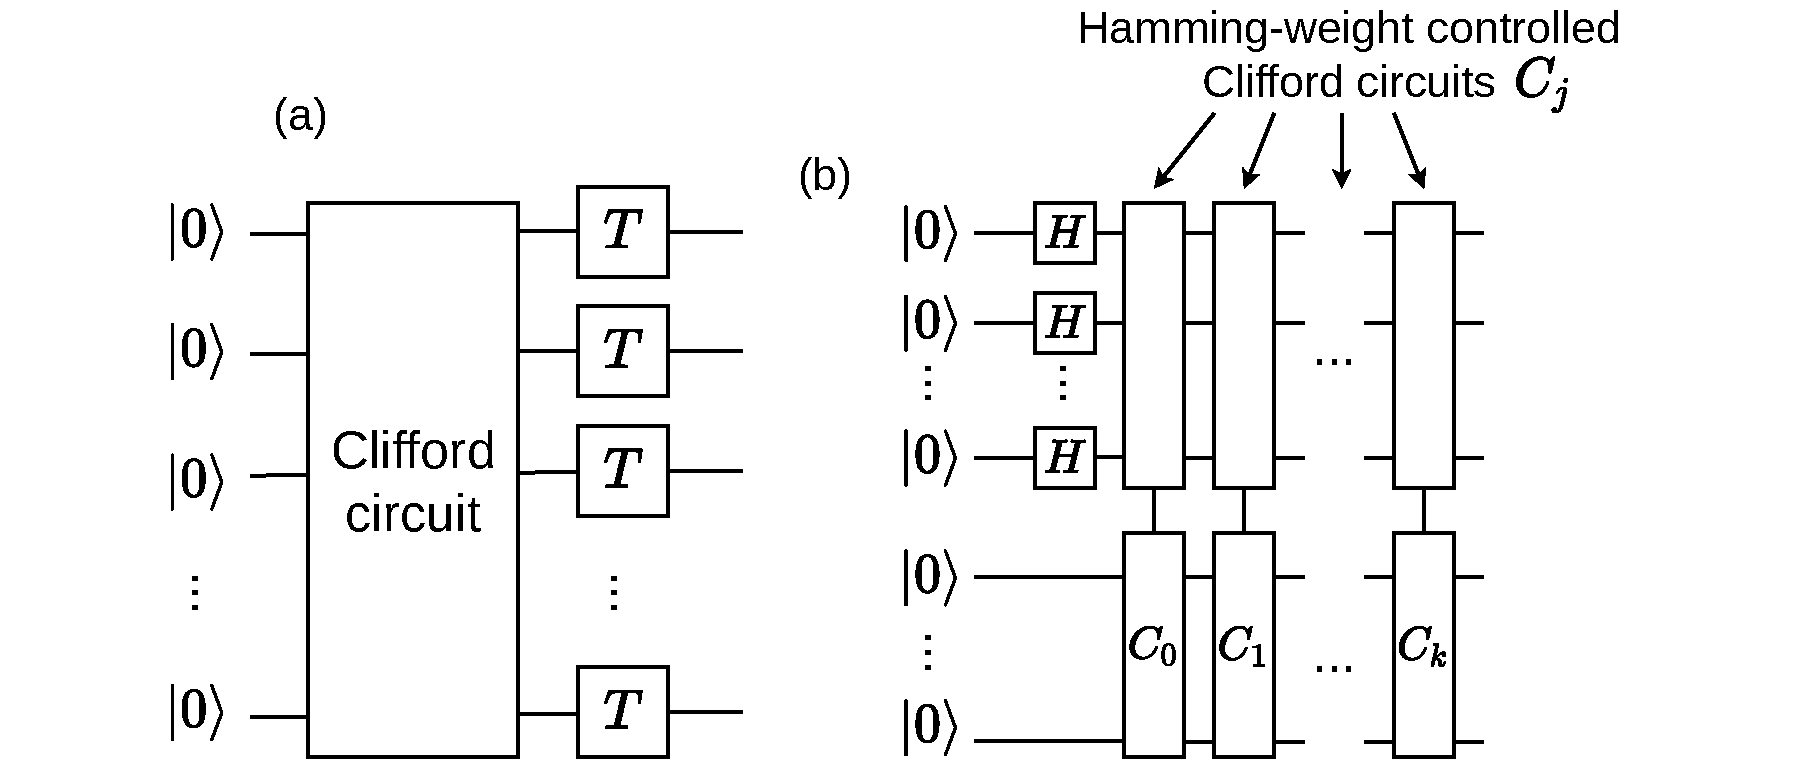
\includegraphics[width=1.0\textwidth]{pics/t-gate-tower.pdf}
	\caption{
		Circuits output a polynomially-size \limdd.
		For (b), the Hamming-weight controlled-$C$ gate on $c$ control qubits and $t$ target qubits maps $\ket{x}\otimes \ket{y}$ to $\ket{x}\otimes C\ket{y}$ if $|x| = 1$ and to $\ket{x}\otimes\ket{y}$ otherwise, for $x\in \{0, 1\}^c$ and $y\in \{0, 1\}^t$.
		Here, $|x| = \sum_{j=1}^c x_j$ denotes the Hamming weight of $x$.
		\todo[inline]{need to explain how to implement Hamming-weight controlled gate?}
		\label{fig:stabilizer-rank-hard}
	}
\end{figure}

 %DEPRECATED
\section{Advanced algorithms}
\label{sec:advanced-algorithms}

\subsection{Measuring an arbitrary qubit}
\label{subsec:measure-arbitrary-qubit}

\autoref{alg:measure-arbitrary-qubit} allows one to measure a given qubit.
Specifically, given a qubit index $k$ and an outcome $y\in \{0,1\}$, it computes the probability of observing $\ket{y}$ when measuring the $k$-th significant qubit.
%\todo[inline]{to do: Add more text ,which explains how/why the algorithm works. -LV}
The algorithm proceeds by traversing the \limdd with root edge $e$ at \autoref{l:traverse1}.
Like \autoref{alg:measurement-top-qubit} which measured the top qubit, this algorithm computes a squared norm.
The case that is added, relative to \autoref{alg:measurement-top-qubit}, is the case when $n>k$, in which case it calls the procedure \textsc{SquaredNormProjected}.
On input $e,y,k$, the procedure \textsc{SquaredNormProjected} outputs the squared norm of $\Pi_k^y\ket{e}$, where $\Pi_k^y$ is the projector which projects the $k$-th qubit onto $\ket{y}$.

\begin{algorithm}[t!]
	\caption{Compute the probability of observing $\ket{y}$ when measuring the $k$-th qubit of the state $\ket{e}$. Here $e$ is given as \limdd on $n$ qubits, $y$ is given as a bit, and $k$ is an integer index.
	For example, to measure the top-most qubit, one calls $\textsc{Measure}(e,0,n)$.
	The procedure $\textsc{SquaredNorm}(e,y,k)$ computes the scalar $\bra{e}(\mathbb I\otimes \ket{y}\bra{y}\otimes \mathbb I)\ket{e}$, i.e., computes the squared norm of the state $\ket{e}$ after the $k$-th qubit is projected to $\ket{y}$. We omit dynamic programming here only for readability.}
	\label{alg:measure-arbitrary-qubit}
	\begin{algorithmic}[1]
		\Procedure{MeasurementProbability}{\Edge
		          $\ledge[e] {\lambda P_n\otimes P^\prime}v$, $y\in \{0,1\}$, $k\in Z_{\geq 1}$}
%		\State (Write $A$ as $A=X^{x}\diagonal{z}\otimes A^\prime$)
		\If{$n=k$}
			\State $p_0:=\textsc{SquaredNorm}(\follow 0e)$
			\State $p_1:=\textsc{SquaredNorm}(\follow 1e)$
			\State \Return $p_j/(p_0+p_1)$ \textbf{where} $j=0$ if $P_n\in\{\mathbb I, Z\}$ and $j=1$ if $P_n \in\set{X,Y}$ 
%			         \Comment{$i = 1$ iff Anti-diagonal}
		\Else
			\State $p_0:=\textsc{SquaredNormProjected}(\follow 0e, y, k)$ \label{l:traverse1}
			\State $p_1:=\textsc{SquaredNormProjected}(\follow 1e, y, k)$
			\State \Return $(p_0+p_1)/\textsc{SquaredNorm}(e)$
		\EndIf
		\EndProcedure
		\Procedure{SquaredNorm}{$\Edge \ledge{\lambda P}{v}$}
			\If{$n=0$}
			%	\State 
			\Return $|\lambda|^2$
			%		\Else
			\EndIf
			\If{$v\in \textsc{Norm-cache}$}
%			\Return $|\lambda|^2\cdot \textsc{Norm-cache}[v]$ \Comment{Dynamic programming}
			\EndIf
			\State $s:=\textsc{Add}(\textsc{SquaredNorm}(\follow 0{\ledge \id v}),\textsc{SquaredNorm}(\follow 1{\ledge \id v}))$
%			\State $\textsc{Norm-cache}[v]:=s$ \Comment{Store in dynamic programming cache}
			\State \Return $|\lambda|^2s$
		\EndProcedure
		\Procedure{SquaredNormProjected}{\Edge $\ledge[e] {\lambda P_n\otimes P'}v$, $y\in\{0,1\}$, $k\in \mathbb Z_{\geq 1}$}
		\State $b:=(P_n \in\set{X,Y})$
						         \Comment{i.e., $b = 1$ iff $P_n$ is Anti-diagonal}
			\If{$n=0$}
				\State \Return $|\lambda|^2$
			\ElsIf{$n=k$}
				\State \Return $\textsc{SquaredNorm}(\follow{b\oplus y}{e})$
%			\ElsIf{$(v,y,k)\in \textsc{NormProj-cache}$}
%				\State \Return $|\lambda|^2\cdot \textsc{NormProj-cache}[v,y,k]$
			\Else
				\State $\alpha_0:=\textsc{SquaredNormProjected}(\follow 0{\ledge {\mathbb I}v}, b\oplus y, k)$
				\State $\alpha_1:=\textsc{SquaredNormProjected}(\follow 1{\ledge {\mathbb I}v}, b\oplus y, k)$
%				\State $\textsc{NormProj-cache}[v,y,k]:=\alpha_0+\alpha_1$
				\State \Return $|\lambda|^2\cdot (\alpha_0+\alpha_1)$
			\EndIf
		\EndProcedure
	\end{algorithmic}
\end{algorithm}



After measurement of a qubit $k$, a quantum state is typically projected to $\ket 0$ or $\ket 1$
 ($b=0$ or $b=1$) on that qubit, depending on the outcome.
\autoref{alg:measure-arbitrary-qubit-update2} realizes this.
It does so by traversing the \limdd until a node $v$ with $\index(v) = k$ is reached.
It then returns an edge to a new node by calling $\makeedge(\low v, 0)$ for projection to $\ket 0$ and  $\makeedge(0, \high v)$ on \autoref{l:project-project},
recreating nodes level $k$ in the backtrack on \autoref{l:project-bt}.
The projection operator $O \defn (\id[n-k] \otimes \ket{b}\bra{b}\otimes \id[k-1])$ commutes with
any LIM $A$ with diagonal operator $P_k$ ($\id[2]$ or $Z$). For the anti-diagonal Pauli operators, we have $O \cdot A \ket v = A \cdot (\id[n-k] \otimes \ket{1-b}\bra{1-b}\otimes \id[k-1])  \ket v$.
The algorithm corrects for this on \autoref{l:project-diag2}.
%\begin{algorithm}
%	\begin{algorithmic}[1]
%		\Procedure{\project}{\Edge $\ledge Av$ \textbf{with} $A=\lambda P_n\otimes\cdots\otimes P_1$, $y\in \{0,1\}$, $k\in \mathbb Z_{\geq 1}$}
%		\State $x= P_n \in \set{X,Y}$    \label{l:project-diag2}  \Comment{flip is $A_k$ is anti-diagonal}     
%		\If{$n= k$}
%			\If{$y=0$} \Return $\textsc{MakeEdge}(\textsc{Project}(e_x,k,x\oplus y), 0)$      \label{l:project-project}
%			\Else\ \Return $\textsc{MakeEdge}(0, \textsc{Project}(e_{1-x},k,x\oplus y))$
%			\EndIf
%		\Else
%			\If{$(v,k,x\oplus y)\in \textsc{Project-cache}$}
%				\State \Return $A\cdot \textsc{Project-cache}[v,k,x\oplus y]$
%			\EndIf
%			\State node $w:=\textsc{MakeEdge}(\textsc{Project}(e_0,k,x\oplus y), \textsc{Project}(e_1,k,x\oplus y))$ \label{l:project-bt}
%			\State $\textsc{Project-cache}[v,k,x\oplus y]:=w$ \Comment{Store the result in the cache}
%			\State \Return $\ledge Aw$
%		\EndIf
%		\EndProcedure
%	\end{algorithmic}
%	\caption{An algorithm which projects the $k$-th qubit to $\ket{y}$. That is, on input $\ledge Av$, the algorithm outputs a \limdd edge representing the state $\mathbb I^{\otimes n-k}\otimes \ket{y}\bra{y}\otimes \mathbb I^{\otimes n-k-1}\ket{\ledge Av}$. This can be used to update a \limdd after a measurement.}
%	\label{alg:measure-arbitrary-qubit-update2}
%\end{algorithm}

\begin{algorithm}
    \begin{algorithmic}[1]
        \Procedure{\project}{\Edge $\ledge {\lambda P_n\otimes .. \otimes P_1}v$, $k\leq n=\index(v)$, $b\in\set{0,1}$}
        \State $b' :=  x \oplus b $ \textbf{where} $x=0$ if $P_k\in\set{\mathbb I,Z}$ and $x=1$ if $P_k\in\set{X,Y}$
        \label{l:project-diag2}  \Comment{flip $b$ if $P_k$ is anti-diagonal}         
        \State \textbf{if} $(v,k, b') \in \cache$ \textbf{then} \Return $\cache[v,k, b']$
         \If{$n = k$}
                \State $e := \makeedge((1- b') \cdot \low v,~~ b' \cdot \high v)$ 
                                                    \Comment{Project $\ket v$ to $\ket{b'}\bra{b'}\otimes \id[2]^{\otimes n-1}$}   
                     \label{l:project-project}
            \Else \Comment{$n \neq k$:}
                \State $e :=\textsc{MakeEdge}(\project(\low v,k, b'),
                                            \project(\high v,k,b'))$ \label{l:project-bt}\vspace{-1em}
             \EndIf
                 \State $\cache[v,k, b'] := e$
                 \State \Return $e$
                \EndProcedure
        \end{algorithmic}
        \caption{Project \limdd \ledge Av to $\ket b$ for qubit $k$, i.e.,
           $(\id[n-k] \otimes \ket{b}\bra{b}\otimes \id[k-1])\cdot \ket{Av}$.}
        \label{alg:measure-arbitrary-qubit-update2}
\end{algorithm}

\subsection{Hadamards on stabilizer states in polynomial time}
\label{sec:hadamard-stabilizer-polytime}

We show that, using the algorithms that we have given, a Hadamard can be applied to a stabilizer state in polynomial time.
We emphasize that our algorithms do not invoke existing algorithms dedicated to applying a Hadamard to a stabilizer state; instead, the \limdd algorithms are inherently polynomial-time for this use case.

\begin{theorem}
	\label{thm:hadamard-stabilizer-polytime}
	\autoref{alg:apply-hadamard}, which applies a Hadamard gate to a stabilizer state represented as a Pauli-\limdd, runs in polynomial time.
\end{theorem}
\begin{proof}
	Let $\ket\phi$ be a stabilizer state, represented by a \limdd with root edge $\ledge Pv$.
	By \autoref{thm:pauli-tower-limdds-are-stabilizer-states}, this \limdd is a Tower Pauli-\limdd.
	\autoref{alg:apply-hadamard} makes two calls to \textsc{Add}; both are of the form $\textsc{Add}(\ledge {\lambda P}v,\ledge{\lambda Qv})$ where $\lambda\in \mathbb C$ is a scalar, $P$ and $Q$ are Pauli strings, and $v$ is a node representing a stabilizer state.
	\autoref{thm:only-linear-recursive-add-calls-general} tells us that at most $8n$ recursive calls to \textsc{Add} are made.
	Each recursive call to \textsc{Add} may invoke the \textsc{MakeEdge} procedure, which runs in time $\mathcal O(n^3)$, yielding a total worst-case running time of $\mathcal O(n^4)$.
\end{proof}

\begin{lemma}
	\label{thm:only-linear-recursive-add-calls}
	Let $v$ be a node in a Tower Pauli-\limdd representing a stabilizer state, and $P$ a Pauli string.
	Then a call to $\textsc{Add}(\ledge {\mathbb I}v,\ledge{P}v)$ invokes only $\mathcal O(n)$ recursive calls~to~\textsc{Add}.
\end{lemma}
\begin{proof}
	Let $v_0,\ldots, v_n$ be the nodes in the Tower Pauli-limdd, with $v=v_n$ the top node and $v_0$ the Leaf node.
	Let $Q^k$ be the label on the high edge from $v_{k+1}$ to $v_k$, for $k=1\ldots n$.
	Let $P=P_n\otimes\cdots\otimes P_1$ and write $P^{(k)}=P_{k}\otimes\cdots\otimes P_1$, so that, e.g., $P=P_n\otimes P_{n-1}\otimes P^{(n-2)}$.
	
	We will show that, upon calling $\textsc{Add}(\ledge{\mathbb I}v,\ledge Pv)$, the recursive calls to \textsc{Add} are all of the form either $\textsc{Add}(\ledge{\mathbb I}{v_k},\ledge{\lambda P^{(k)}}{v_k})$, or $\textsc{Add}(\ledge{Q^k}{v_{k}},\ledge{\lambda P^{(k)}Q^k}{v_{k}})$ with $\lambda\in \{\pm 1,\pm i\}$.
	Let us first note how the lemma would follow from this fact.
	If these are the only ways in which the algorithm is called, then there are only $8n$ different parameters with which the algorithm is invoked.
	Because the algorithm uses a cache in which it stores the result of each computation, it will not descend into recursive calls after a cache hit.
	Therefore, only at most $8n$ recursive calls to \textsc{Add} are made after the initial call.
	
	First, suppose the algorithm is invoked as $\textsc{Add}(\ledge{\mathbb I}{v_k},\ledge{\lambda P^{(k)}}{v_k})$.
	If this yields a cache hit, the algorithm halts without recursing; otherwise, the following two recursive calls to \textsc{Add} are made,
	\begin{align}
		\label{eq:add-call-0}
		&\textsc{Add}(\follow0{\ledge {\mathbb I}{v_k}},\follow0{\ledge {P^{(k)}}{v_k}}) \\
		\label{eq:add-call-1}
		\text{and } & \textsc{Add}(\follow 1{\ledge {\mathbb I}{v_k}},\follow 1{\ledge {P^{(k)}}{v_k}})
	\end{align}
	We note that $\follow 0{\ledge{\mathbb I}{v_k}}=\ledge{\mathbb I}{v_{k-1}}$ and $\follow 1{\ledge{\mathbb I}{v_k}}=\ledge {Q^{k-1}}{v_{k-1}}$.
	The value of $\follow b{\ledge {P^{(k)}}{v_k}}$ depends on the value of $P_k$, so we distinguish four cases.
	\begin{enumerate}[(a)]
		\item \textbf{Case} $P_n=\mathbb I$.
		Then $P\ket{v_k} = \ket 0P^{(k-1)}\ket{v_{k-1}}+\ket 1P^{(k-1)}\ket{v_{k-1}}$, so we have $\follow0{\ledge Pv}=P^{(k-1)}\ket{v_{k-1}}$ and $\follow 1{\ledge {P^{(k)}}v}=P^{(k-1)}\ket{v_{k-1}}$, as above.
		\item \textbf{Case} $P_n=X$.
		Then $P\ket{v_k}=\ket 0P^{(k-1)}Q^n\ket{v_{k-1}} + \ket 1P^{(k-1)}\ket{v_{k-1}}$, so we have $\follow 0{\ledge {P^{(k)}}{v_k}}=\ledge{P^{(k-1)}Q^k}{v_{k-1}}$ and $\follow 1{\ledge {P^{(k)}}{v_k}}=\ledge{P^{(k-1)}}{v_{k-1}}$.
		\item \textbf{Case} $P_n=Y$.
		Then $P\ket{v_n} = -i\ket 0P^{k-1}\ket{v_{k-1}}+i\ket 1P^{(k-1)}Q^{k-1}\ket{v_{k-1}}$, so we have $\follow0{\ledge {P^{(k)}}{v_k}}=\ledge {-iP^{(k-1)}}{v_{k-1}}$ and $\follow 1{\ledge {P^{(k)}}{v_k}}=\ledge{iP^{(k-1)}Q^k}{v_{k-1}}$.
		\item \textbf{Case} $P_n=Z$.
		Then $P\ket{v_k} = \ket 0P^{(k-1)}\ket{v_{k-1}}-\ket 1P^{(k-1)}Q^{k-1}\ket{v_{k-1}}$, so we have $\follow0{\ledge {P^{(k)}}{v_k}}=\ledge{P^{(k-1)}}{v_{k-1}}$ and $\follow1{\ledge {P^{(k)}}{v_k}}=\ledge{-P^{(k-1)}Q^{k-1}}{v_{k-1}}$.
	\end{enumerate}
	In each case, indeed the two recursive calls to \textsc{Add} of Equations \ref{eq:add-call-0} and \ref{eq:add-call-1} are of the form indicated.

	Next, suppose that the algorithm is called as $\textsc{Add}(\ledge{Q^k}{v_{k}},\ledge{\lambda P^{(k)}Q^k}{v_{k}})$.
	Then, on line \ref{algline:add-factor-out-LIM} of the \textsc{Add} algorithm, a LIM $C$ is built such that $C\ket{v_k}=\lambda Q^{k,-1}P^{(k)}Q^k\ket{v_k}$.
	Then the algorithm proceeds as though it was called with $\textsc{Add}(\ledge{\mathbb I}{v_k},\ledge C{v_k})$.
	The LIM $C$ satisfies $C\ket{v_k}=\pm \lambda P^{(k)}\ket{v_k}$.
	By the observations above, this case, too, will yield only recursive calls to \textsc{Add} of the specified form.
\end{proof}

\begin{corollary}
	\label{thm:only-linear-recursive-add-calls-general}
	Let $v$ be a node in a Tower Pauli-\limdd representing a stabilizer state, $P,Q$ Pauli strings, and $\lambda\in \mathbb C$ a scalar.
	Then a call to $\textsc{Add}(\ledge {\lambda P}v, \ledge {\lambda Q}v)$ invokes only $\mathcal O(n)$ recursive calls to \textsc{Add}.
\end{corollary}
\begin{proof}
	If $P=\mathbb I$, then this is the same as \autoref{thm:only-linear-recursive-add-calls}.
	Otherwise, the \textsc{Add} procedure factors out the LIM $\lambda P$ and proceeds as though it were called as $\textsc{Add}(\ledge{\mathbb I}v,\ledge{PQ}v)$, which is the case treated by \autoref{thm:only-linear-recursive-add-calls}.
\end{proof}


%\subsection{General ApplyGate algorithm}
%\label{sec:apply-gate-limdd-limdd}
%
%\autoref{alg:apply-gate-limdd-limdd-cache} applies a gate to a state, allowing one to simulate a quantum circuit, just like \autoref{alg:apply-gate-limdd-limdd}.
%By storing a different tuple in the cache than \autoref{alg:apply-gate-limdd-limdd}, it is able to better take advantage of dynamic programming. It proceeds exactly like the \textsc{ApplyGate} algorithm explained in \autoref{sec:apply-gate-limdd-limdd}.
%
% \todo{This seems incorect and we do not need it -AL}
%
%%\todo[inline]{Add more explanation or replace with a note in the main text ``we could actually cache modulo...'' -AL}
%
%\begin{algorithm}
%	\caption{Applies the gate $[e^U]$ to the state $\ket{e^v}$. Here $e^U$ and $e^v$ are \limdd edges.
%	The output is a \limdd edge $e^\Psi$ satisfying $\ket{e}=[e^U]\ket{e^v}$.}
%	\label{alg:apply-gate-limdd-limdd-cache}
%	\begin{algorithmic}[1]
%		\Procedure{ApplyGate}{\Edge $e^U=\ledge BU$ \textbf{with} $B=\lambda_B Q_{2n}\otimes\cdots\otimes Q_1$, \Edge $e^v=\ledge Av$ \textbf{with} $A=\lambda_A P_n\otimes\cdots\otimes P_1$}
%			\If{$A=0$ or $B=0$} \Return $0$
%			\EndIf
%			\If{$n=0$}
%				\State \Return $\ledge {AB}v$
%			\Else
%				\State $R:=\rootlabel((Q_{2n-1}^\top P_n)\otimes (Q_{2n-3}^\top P_{n-1})\otimes\cdots\otimes (Q_1^\top P_1), e^v)$
%				\If{$(U,\ledge Rv)\in \textsc{Apply-cache}$}\Comment{Dynamic programming}
%					\State \Return $\lambda_A \lambda_B (Q_{2n}^\top\otimes Q_{2n-2}^\top\otimes\cdots\otimes Q_2^\top)\cdot \textsc{Apply-cache}[U, \ledge Rv]$
%				\EndIf
%%				\State edge $a_0:=\follow{0}{e^v}$
%%				\State edge $a_1:=\follow{1}{e^v}$
%				\For{$r,c\in\{0,1\}$}
%%					\State edge $M_{r,c}:=\follow{rc}{e^U}$
%%				\EndFor
%%				\For{$r,c\in \{0,1\}$}
%					\State \Edge $\Psi_{r,c}:=\textsc{ApplyGate}(\follow{rc}{\ledge {\mathbb I_2^{\otimes n}}{U}},\follow{c}{\ledge Rv})$
%				\EndFor
%				\State \Edge $e_0:=\textsc{Add}(\Psi_{0,0}, \Psi_{0,1})$
%				\State \Edge $e_1:=\textsc{Add}(\Psi_{1,0}, \Psi_{1,1})$
%				\State \Edge $e^\Psi:=\textsc{MakeEdge}(e_0,e_1)$
%				\State $\textsc{Apply-cache}[U, \ledge Rv]:=e^\Psi$ \Comment{Store result in cache}
%%				\State Store $(e^v,e^U, e^\Psi)$ in the \textsc{Apply-cache}
%				\State \Return $\lambda_A\lambda_B (Q_{2n}^\top\otimes Q_{2n-2}^\top\otimes\cdots\otimes Q_2^\top)\cdot e^\Psi$
%			\EndIf
%		\EndProcedure
%	\end{algorithmic}
%\end{algorithm}

%\begin{algorithm}
%	\caption{An implementation of the \textit{follow} function. On input $e,y$, with $\ket{e}=\ket{0}\ket{e_0}+\ket{1}\ket{e_1}$, it outputs an edge to a \limdd $f$ such that $\ket{f}=\ket{e_y}$.}
%	\label{alg:partial-expand}
%	\begin{algorithmic}[1]
%		\Procedure{Follow}{\Edge $e=(\cdot, A,v)$, $y\in \{0,1\}$}
%			\State (Let $x,z,A^\prime$ be such that $A=X^x\diagonal{z}\otimes A^\prime$)
%			\If{$y=0$}
%				\State \Return $z^xA^\prime\ket{e_x^v}$
%			\Else
%				\State \Return $z^{1-x}A^\prime\ket{e_{1-x}^v}$
%			\EndIf
%		\EndProcedure
%		\Procedure{Follow}{edge $e$, $i\in \{0,1\}$, $j\in \{0,1\}$}
%			\State \Return $\textsc{}(\textsc{Follow}(e, i), j)$
%		\EndProcedure
%	\end{algorithmic}
%\end{algorithm}

%\begin{algorithm}
%	\caption{Produces a new \glimdd with a new variable order, by swapping the qubits $q_k$ and $q_{k+1}$. Namely, if the edge $e$ has the order $q_1,q_2,\ldots, q_n$, then we produce a new \glimdd with variable order $q_1,q_2,\ldots,q_{k-2},q_k,q_{k-1},q_{k+1},q_{k+2},\ldots, q_n$.}
%	\label{alg:swap-qubits}
%	\begin{algorithmic}[1]
%		\Procedure{SwapQubits}{\glimdd edge $e$, qubit $k$}
%			\State (to do)
%		\EndProcedure
%	\end{algorithmic}
%\end{algorithm}

%\input{sections/non-diagonal-groups.tex}
%\section{Correctness proof of Algorithms~\ref{alg:findisointersection}, \ref{alg:getautomorphisms} and \ref{alg:getsingleisomorphism}}

\todo[inline]{rewrite \& check if all references to algorithm contents are still correct}

Here, we prove that \findisomorphismsetintersection~is correct, for which we need the following remark and lemma.

\begin{remark}
    \label{remark:correctness-isomorphism-intersection}
    If $I$ is an \isomorphismset, then denote by $\pi_I$ the single isomorphism and by $G_I$ the \automorphismgenerators~object it contains.
    Furthermore, denote by $\langle G\rangle$ the automorphism group generated by $G$.
    Upon input $I_A, I_B$ and output $I$, the correctness criterion of the function \findisomorphismsetintersection~is equivalent to 
    \[
        \pi_{I} \cdot \langle G \rangle = \left( \pi_{I_A} \cdot \langle G_{I_A} \rangle \right) \cap \left( \pi_{I_B} \cdot \langle G_{I_B} \rangle \right)
    \]
    where we have denoted $\pi \cdot G = \{\pi \cdot g \mid g \in G\}$.
\end{remark}


\begin{lemma}
    \label{thm:coset-intersection-nonempty}
    Let $G$ be a group with subgroups $G_A$ and $G_B$, and let $\pi_A, \pi_B \in G$.
    The intersection $(\pi_A \cdot G_A)\cap (\pi_B \cdot G_B)$ is nonempty if and only if $\pi_A^{-1} \pi_B$ can be written as $\pi_A^{-1}\pi_B=g_A \cdot g_B$, for some $g_A \in G_A$ and $g_B \in G_B$.
\end{lemma}
\begin{proof}
    \todo[inline]{fill (with proof that Lieuwe wrote before)}
\end{proof}

Now we prove that the algorithm \findisomorphismsetintersection~is correct.

\begin{lemma}
    The function \findisomorphismsetintersection~satisfies its correctness criterion given in 
    \cref{remark:correctness-isomorphism-intersection}.
\end{lemma}
\begin{proof}
    First, we start by using the well-known fact that the intersection of two cosets $\pi_{I_A} \cdot \langle G_{I_A} \rangle$ and $\pi_{I_B} \cdot \langle G_{I_B} \rangle$ is either empty, or it is a coset of $\langle G_{I_A} \rangle \cap \langle G_{I_B} \rangle$.
    Hence, the algorithm is correct if 
    \begin{enumerate}[(a)]
        \item the \automorphismgenerators~object it outputs is $\langle G_{I_A} \rangle \cap \langle G_{I_B} \rangle$;
        \item the single isormorphism it outputs is an element of $\left( \pi_{I_A} \cdot \langle G_{I_A} \rangle \right) \cap \left( \pi_{I_B} \cdot \langle G_{I_B} \rangle \right)$, or \none~if this intersection is empty.
    \end{enumerate}

    We first prove (a).
    The central insight is that the removal of elements containing $X$ or $Y$ from $H_B^{\textnormal{echelon}}$ in step 7 does not alter the intersection we aim for. That is:
    \begin{equation}
        \label{eq:noXY}
    \langle H_A \rangle \cap \langle H_B^{\textnormal{echelon}} \rangle = 
    \langle H_A \rangle \cap \langle H^{\textnormal{noXY}}_B \rangle
        .
    \end{equation}
    The reason why this holds is that elements of $H_A$ do not contain $X$ or $Y$, while for each $k \in \{1, 2, \dots n\}$, there is at most a single operator in $H_B^{\textnormal{echelon}}$ which contains a pivot at position $k$ which is either $X$ or $Y$; therefore, no element in $\langle H_A\rangle \cap \langle H_B^{\textnormal{echelon}}\rangle$ will have a decomposition in $H_B^{\textnormal{echelon}}$ containing operators containing $X$ or $Y$.
    \todo[inline]{argument is simpler than I manage to put into words; add picture to clarify the argument?}

    Let us now prove the (a).
    We use the notation $U^{\dagger} A U = \{U^{\dagger} a U | a \in A\}$ where $A$ is an arbitrary set.
    Following the notation from the algorithm,
    \begin{eqnarray*}
        \langle G\rangle
        &=&
        U^{\dagger} \left(
        \langle H_A \rangle \cap \langle H_B^{\textnormal{noXY}}\rangle
        \right) U
        \\
        &\stackrel{\textnormal{eq.~\eqref{eq:noXY}}}{=}&
        U^{\dagger} \left(
        \langle H_A \rangle \cap \langle H_B^{\textnormal{echelon}}\rangle
        \right) U
        \\
        &=&
        U^{\dagger} \left(
        \langle H_A \rangle \cap \langle H_B\rangle
        \right) U
        \\
        &=&
        U^{\dagger} \left(
        \langle U G_A U^{\dagger} \rangle \cap \langle U G_B U^{\dagger}\rangle
        \right) U
        \\
        &\stackrel{*}{=}&
        U^{\dagger} U \left(
        \langle G_A \rangle \cap \langle G_B\rangle
        \right) U^{\dagger} U
        \\
        &=&
        \langle G_A \rangle \cap \langle G_B\rangle
    \end{eqnarray*}
    where $\stackrel{*}{=}$ holds because the map $x \mapsto Ux U^{\dagger}$ is a group isomorphism.

    We prove (b) by showing the following two statements: (b1) if the single isomorphism that is outputted by the isomorphism is not \none, then it is an element of the intersection of $\pi_{I_A} \cdot \langle G_{I_A} \rangle$ and $\pi_{I_B} \cdot \langle G_{I_B} \rangle$, and (b2) if the outputted isomorphism is $\none$, then this intersection is empty.

    Proving (b1) is straightforward: from step 8 of the algorithm we see that 
    \begin{equation}
        \label{eq:tau-prime-1}
   \tau' = \prod_{j} h_j^A \cdot \prod_{k} h_k^B
    \end{equation}
    where $h_j^A \in H_A, h_k^B\in H_{B}^{\textnormal{noXY}}$
    while from steps 1--5 we observe that $\tau'$ can also be written as
    \begin{equation}
        \label{eq:tau-prime-2}
        \tau' = U\pi_A^{-1} U^{\dagger} U \pi_B U^{\dagger} \cdot \prod_{\ell} h_{\ell}^{\textnormal{echelon}}
    \end{equation}
 for $h_{\ell}^{\textnormal{echelon}} \in \langle H_B^{\textnormal{echelon}} \rangle = \langle H_B \rangle$.
    Combining eqs.~\eqref{eq:tau-prime-1} and~\eqref{eq:tau-prime-2} and reshuffling yields
    \begin{equation}
        \label{eq:tau-prime-3}
        U \pi_B U^{\dagger} \cdot \prod_{\ell} h_{\ell}^{\textnormal{echelon}}  \cdot \prod_{k} \left(h_k^B\right)^{-1}
        =
        U\pi_A U^{\dagger} \cdot \prod_{j} h_j^A
    \end{equation}
    Applying the group isomorphism $x \mapsto U^{\dagger} x U$ to both sides of eq.~\eqref{eq:tau-prime-3}, we find
    \[
        \pi_B \cdot \prod_{\ell} U^{\dagger} h_{\ell}^{\textnormal{echelon}} U  \cdot \prod_{k} U^{\dagger} \left(h_k^B\right)^{-1} U
        =
        \pi_A \cdot \prod_{j} U^{\dagger} h_j^A U
    \]
    Since $H_A = \{UgU^{\dagger} | g \in G_A\}$ and similary for $H_B$ we infer that
    \[
        \pi_A \cdot \prod_{j} U^{\dagger} h_j^A U \in 
    \]
    is an element of
    both
    $\pi_{I_A} \cdot \langle G_{I_A} \rangle$
    and
    $\pi_{I_B} \cdot \langle G_{I_B} \rangle$
    , which proves (b1).

    For proving (b2), we note that the algorithm outputs \none~precisely if $\tau'$ cannot be written as $h_A \cdot h_B$ where $h_{\Box} \in \langle H_{\Box} \rangle$.
    To see this, consider the two steps in the algorithm where \none~is returned:
    \begin{itemize}
        \item in step 6; $\tau'$ contains at least one $X$ or $Y$ which has not been eliminated in step 5, while $H_A$ only contains $Z$ and $\unit_2$, so $\tau'\notin \langle H_A \rangle \cdot \langle H_B \rangle$.\todo[inline]{maybe needs more rigorous proof}
        \item in step 8, where the Zassenheim algorithm finds a decomposition of $\tau'$ of the form $h_A \cdot h_B$ only if it exists.
    \end{itemize}
It follows from the fact that $\tau'$ is not an element of $\langle H_A \rangle \cdot \langle H_B \rangle$ that $\tau$ is neither, and using the fact that $x\mapsto UxU^{\dagger}$ is a group isomorphism, we find by definition of $\tau$ that $\pi_A^{-1} \pi_B \notin \langle G_A \rangle \cdot \langle G_B\rangle$.
    It now follows from Lemma~\ref{thm:coset-intersection-nonempty} that the intersection between $\pi_A\cdot \langle G_A \rangle$ and $\pi_B\cdot \langle G_B \rangle$ is empty, which concludes the proof for (b2).
\end{proof}





\begin{lemma}[Conditional correctness of function \getautomorphisms]
    \label{lemma:condition-correctness-1}
    The function \getautomorphisms~satisfies its correctness criterions for single-qubit states.
    Moreover, it also does so for $n$-qubit states for $n>1$, conditioned on the correctness of the function \getsingleisomorphism~for quantum states on strictly fewer than $n$ qubits.
\end{lemma}
\begin{proof}
    In case two states are given as input, then the correctness of the algorithm is an immediate consequence of the correctness of the single-state-input case and the correctness of the algorithm \findautomorphismsetintersection.
    So we only need to prove the case where a single state is given as input.
    We use induction on the number of qubits $n$.
    The case $n=1$ is a brute-force search over the (six) single-qubit stabilizer states and is thus correct.
    For the case $n>1$, we show the following two statements:

    (i) each operator that is outputted by \getautomorphisms~is an automorphism of $\ket{\phi}$;

    (ii) each automorphism of $\ket{\phi}$ can be written as product of operators outputted by \getautomorphisms.

    Showing (i) is straightforward, assuming that \getsingleisomorphism~and \getautomorphisms~are both correct for $(n-1)$-qubit states.
    For example, for the operators of the form $\unit_2\otimes g$ with $g$ an automorphism to both $\ket{\phi_0}$ and $\ket{\phi_1}$, we write
    \begin{eqnarray*}
        \unit_2 \otimes g \ket{\phi}
        =
        \alpha_0 \ket{0} \otimes g\ket{\phi_0} + \alpha_1 \ket{1} \otimes g\ket{\phi_1}
        =
        \alpha_0 \ket{0} \otimes \ket{\phi_0} + \alpha_1 \ket{1} \otimes \ket{\phi_1}
        = \ket{\phi}
        .
    \end{eqnarray*}
    The other three cases are similar.

    Regarding (ii), we first note that if $\unit_2 \otimes g$ is an automorphism of $\ket{\phi}$, then $
    \alpha_0 \ket{\phi_0} =
    \left(\bra{0}\otimes \unit_{2^{n-1}}\right) \left(\unit_2 \otimes g \ket{\phi}\right) =
    g (\alpha_0 \ket{\phi_0})
    $
    and hence $g$ must be an automorphism to $\ket{\phi_0}$, while following a similar argument $g$ is also an automorphism to $\ket{\phi_1}$.
    This shows that all automorphisms of the form $\unit_2 \otimes g$ are in the output of \getautomorphisms.
    Regarding automorphisms of the form $X\otimes a$ with $a$ an $(n-1)$ qubit Pauli operator, it is not hard to see that $a$ is an isomorphism mapping $\alpha_0 \ket{\phi_0}$ to $\alpha_1 \ket{\phi_1}$ and vice versa.
    Now note that $X\otimes a = (X\otimes s)(\unit_2 \otimes s a)$ where $s$ is as in the algorithm.
    Since $s$ maps $\alpha_0 \ket{\phi_0}$ to $\alpha_1 \ket{\phi_1}$, we see that $sa$ is an automorphism to both $\ket{\phi_0}$ and $\ket{\phi_1}$, so that $X\otimes a$ can be written as product of elements outputted by \getautomorphisms.
    The argument for the remaining two cases, i.e. automorphisms of the form $Z\otimes a$ and $Y\otimes a$, are similar.
    This finishes the proof for (ii).
\end{proof}


\begin{lemma}[Conditional correctness of function \getsingleisomorphism]
    \label{lemma:condition-correctness-2}
    The function \getsingleisomorphism~satisfies its correctness criterions for $0$-qubit states.
    Moreover, it also does so for $n$-qubit states for $n>0$, conditioned on the correctness of the function \getautomorphisms~for quantum states on strictly fewer than $n$ qubits.
    \todo[inline]{Readers might $0$-qubit states find confusing...Reason we chose it is because starting the recursion at 0 qubits gives a concise formulation than at 1 qubit}
\end{lemma}
\begin{proof}
    If the input are $0$-qubit states, then correctness is immediate, both for single- and two-tuple input.
    For the case of $n$-qubit input states with $n>0$, correctness of the two-tuple case follows immediately from the correctness of the functions \getautomorphisms~(on $n$ qubits) and \findisomorphismsetintersection.
    The case $n>0$ for the single-tuple input case is also correct since the algorithm is a brute-force search over the four single-qubit Pauli operators on the most-significant qubit.
\end{proof}

By induction on the number of qubits, the correctness of the algorithm \getsingleisomorphism~now follows straighforwardly from Lemma~\ref{lemma:condition-correctness-1} and \ref{lemma:condition-correctness-2}.

\begin{corollary}[Unconditional correctness of function \getsingleisomorphism]
    The function \getsingleisomorphism~satisfies its correctness criterions.
\end{corollary}



\section{Correctness proof of \textsc{GetCanonicalLabels}}
\label{sec:proof-getcanonicallabels}

\todo[inline]{TODO}


\begin{lemma}
    \label{lemma:automorphism-phase}
    If $\lambda P$ is an element of a Pauli automorphism group, then $\lambda \in \{\pm 1\}$.
\end{lemma}
\begin{proof}
    Let $\lambda P$ be an element of the automorphism group of a state $\ket{\phi}$.
    Then $\lambda^2 \ket{\phi} = (\lambda P)^2 \ket{\phi} = \lambda P (\lambda P \ket{\phi}) = \lambda P \ket{\phi} = \ket{\phi}$, so $\lambda^2 = 1$, so $\lambda \in \{\pm 1\}$.
\end{proof}

\begin{lemma}
    Let $G_0, G_1$ be Pauli automorphism groups and $G = \langle G_0 \cup G_1 \rangle$.
    If $g\in G$, then $\pm i g \notin G$.
\end{lemma}
\begin{proof}
    To reach a contradiction, assume there exists a $g\in G$ for which $\pm i g \in G$ also.
    Since Pauli LIMs commute or anticommute, we can decompose both as $g = (-1)^x g_0 g_1$ and $\pm i g = (-1)^y h_0 h_1$ for some $x, y \in \{0, 1\}$ and $g_0, h_0\in G_0$ and $g_1, h_1 \in G_1$.
    Combining yields $\pm i (-1)^x g_0 g_1 = (-1)^y h_0 h_1$, which we rewrite as $\pm i (-1)^{x+y} \underbrace{g_1 h_1^{-1}}_{\in G_1} = \underbrace{g_0^{-1} h_0}_{\in G_0}$. 
    Squaring both sides yields the contradiction $-1 \cdot \id[2] = \id[2]$ where we used that automorphisms square to $\id[2]$ (corollary of \autoref{lemma:automorphism-phase}).
\end{proof}

\begin{corollary}
    Let $G_0, G_1$ be Pauli automorphism groups and $G = \langle G_0 \cup G_1 \rangle$.
    If $\lambda P \in G$ and $\mu P \in G$, then $\lambda = \pm \mu$.
\end{corollary}




% % % % % DEPRECATED these sections do not go into the final manuscript % % % % %
%\input{sections/app_quantum101.tex}
%\tableofcontents

\end{document}
